\documentclass{scrbook}
\usepackage{makeidx}
\usepackage{style}

\pagestyle{scrheadings}
\usepackage[
toc,          %go to table of contents
section]      %in table of contents in chapter-level
{glossaries}

\subject{Skriptum}
\title{107.A04 Wahrscheinlichkeitstheorie und stochastische Prozesse 
für Informatik 4.0}
\author{Karl Grill}
\uppertitleback{Unter Creative Commons Attribution Sharealike Lizenz}
\lowertitleback{\copyright 2013, 2014  Karl Grill}
\date{24.1.2014}
\publishers{Institut für Statistik und Wahrscheinlichkeitstheorie TU Wien}

\makeatletter
\AtBeginDocument{
    \hypersetup{
        pdftitle = {\@title},
        pdfsubject={\@subtitle},
        pdfauthor={\@author},
        pdfproducer={Latex (Debian/GNU Linux)},
        pdfkeywords={\@title, \@subject}
    }
}
\makeatother

%do some kind of magic :-)
\setcounter{tocdepth}{4}
\ExerciseLevelInToc{subsubsection}

%symbollist create
\newglossary[slg]{symbolslist}{syi}{syg}{Symbolverzeichnis}
\renewcommand*{\glspostdescription}{}%remove trailing dot
\makeglossaries

\newglossaryentry{symb:Omega}{
    name=$\Omega$,
    description={Grundgesamtheit (auch Grundmenge $M$), die Menge ihrer Untersuchungseinheiten $\omega$.},
    sort=symbolOmega, type=symbolslist
}

\newglossaryentry{symb:omega}{
    name=$\omega$,
    description={Umtersuchungseinheit (Element) der Grundgesamtheit $\Omega$},
    sort=symbolomega, type=symbolslist
}

\newglossaryentry{symb:emptyset}{
    name=$\emptyset$,
    description={Die leere Menge},
    sort=symbolemptyset, type=symbolslist
}

\newglossaryentry{symb:theta}{
    name=$\theta$,
    description={Der Parameter eines parametrischen Modells (kann Mehrdimensional sein) $\theta\subset\Theta$},
    sort=symboltheta, type=symbolslist
}

\newglossaryentry{symb:Theta}{
    name=$\Theta$,
    description={Der Parameterraum $\theta\subset\Theta$.},
    sort=symbolTheta, type=symbolslist
}

\newglossaryentry{symb:hatthetan}{
    name=$\hat\theta_n$,
    description={Schätzer, eine Folge von Statistiken},
    sort=symbolthetahatn, type=symbolslist
}

\newglossaryentry{symb:alpha}{
    name=$\alpha$,
    description={Wahrscheinlichkeit des $\alpha$-Quantils},
    sort=symbolalpha, type=symbolslist
}

\newglossaryentry{symb:alphafehler}{
    name=$\alpha$,
    description={Wahrscheinlichkeit für einen Fehler 1.Art},
    sort=symbolalphafehler, type=symbolslist
}

\newglossaryentry{symb:betafehler}{
    name=$\beta$,
    description={Wahrscheinlichkeit für einen Fehler 2.Art},
    sort=symbolbetafehler, type=symbolslist
}

\newglossaryentry{symb:gamma}{
    name=$\gamma$,
    description={Überdeckungswahrscheinlichkeit eines Konfidenzintervalls},
    sort=symbolgamma, type=symbolslist
}

\newglossaryentry{symb:zalpha}{
    name=$z_\alpha$,
    description={$\alpha$-Quantil der Standardnormalverteilung},
    sort=symbolzalpha, type=symbolslist
}

\newglossaryentry{symb:mathbbE}{
    name=$\mathbb E$,
    description={Erwartungswert},
    sort=symbolEmathbb, type=symbolslist
}

\newglossaryentry{symb:mu}{
    name=$\mu$,
    description={Erwartungswert},
    sort=symbolmu, type=symbolslist
}

\newglossaryentry{symb:mathbbV}{
    name=$\mathbb V$,
    description={Varianz},
    sort=symbolVmathbb, type=symbolslist
}

\newglossaryentry{symb:mathbbP}{
    name=$\mathbb P$,
    description={Wahrscheinlichkeit},
    sort=symbolPmathbb, type=symbolslist
}

\newglossaryentry{symb:iid}{
    name={i.i.d.},
    description={independent and identically distributed},
    sort=symboliid, type=symbolslist
}

\newglossaryentry{symb:alphaunder}{
    name=$\uline\alpha$,
    description={Anfangsverteilung},
    sort=symbolalphaunderline, type=symbolslist
}

\newglossaryentry{symb:piunder}{
    name=$\uline\pi$,
    description={stationäre Verteilung},
    sort=symbolpiunderline, type=symbolslist
}

\newglossaryentry{symb:H}{
    name=$H$,
    description={$H(P)$ Entropie},
    sort=symbolH, type=symbolslist
}

\newglossaryentry{symb:Hstar}{
    name=$H^*$,
    description={$H*(P)$ Mittlere Unbestimmtheit},
    sort=symbolHstar, type=symbolslist
}

\newglossaryentry{symb:m}{
    name=$m$,
    description={Anzahl der Blätter im Baum/die Anzahl der Zufallsvariablen},
    sort=symbolm, type=symbolslist
}

\newglossaryentry{symb:I}{
    name=$I$,
    description={$I_x=I(p_x)$ Informationsgehalt},
    sort=symbolI, type=symbolslist
}

\newglossaryentry{symb:sn2}{
    name=$s_n^2$,
    description={(korrigierte) Stichprobenvarianz},
    sort=symbolsn2, type=symbolslist
}

\newglossaryentry{symb:varphi}{
    name=$\varphi$,
    description={Dichte der Standardnormalverteilung},
    sort=symbolsvarphi, type=symbolslist
}

\newglossaryentry{symb:Phi}{
    name=$\Phi$,
    description={Verteilungsfunktion der Standardnormalverteilung},
    sort=symbolsPhi, type=symbolslist
}

\makeindex

\clearscrheadfoot%define own even-odd positions for page-numbers
\lohead[\leftmark]{\leftmark}
\rehead[\rightmark]{\rightmark}
\refoot[\pagemark]{\pagemark}
\lofoot[\pagemark]{\pagemark}

\begin{document}
\maketitle
\tableofcontents
{
    \chapter{Grundlagen der Wahrscheinlichkeitstheorie}\index{Wahrscheinlichkeitstheorie|(}
    \section{Die Axiome von Kolmogorov}\index{Kolmogorov Axiome|see {Axiome von Kolmogorov}}\index{Axiome von Kolmogorov|(}

    Für das erste Beispiel im Gebiet der Wahrscheinlichkeitstheorie rollen
    wir zwei Würfel.\\

    \begin{minipage}{\linewidth}
        \centering
        \def\svgwidth{2cm}
        \input{chapters/wahrscheinlichkeitstheorie/dices.pdf_tex}\\\tiny{Steaphan Greene, CC BY-SA 3.0}
    \end{minipage}

    \begin{definition}
    Alle möglichen Ausgänge kombiniert,nennen wir \textbf{Grundmenge}.
    \end{definition}

    \textbf{Grundmenge\index{Grundmenge} $M\text{ bzw. }\Omega$}\\

    Die Grundmenge $M\text{ bzw. }\Omega$ besteht aus dem Produkt der Ausgänge von Würfel A und der Ausgänge von Würfel B:\\
    Würfel A: $A=\{1,2,3,4,5,6\}$\\
    Würfel B: $B=\{1,2,3,4,5,6\}$

    \begin{equation*}
        M=\Omega =A\times B=\{\left(1,1\right),\left(1,2\right),\ldots,\left(3,4\right),\ldots ,\left(6,6\right)\}
    \end{equation*}
    
    Egal was gewürfelt wird, unser Ergebnis ist bereits in der Grundmenge M. 
    Die Wahrscheinlichkeit \gls{symb:mathbbP} dass das Ergebnis in der Grundmenge
    liegt, ist 100\%.

    \begin{equation*}
        \mathbb{P}\left(M\right)=\mathbb{P}(\Omega )=1
    \end{equation*}

    \textbf{Elementarereignis}\index{Elementarereignis}\\
    Ein einzelner Ausgang, also z.B. $(2,5)$, wird Elementarereignis genannt.\\

    \textbf{Leere Menge \gls{symb:emptyset}}\index{Leere Menge}

    Eine leere Menge enthält kein Element. Findet jedoch ein Zug statt (z.B.
    Würfel fallen), entsteht mit Gewissheit ein Ergebnis.

    \begin{equation*}
        \mathbb{P}\left({\emptyset}\right)=0
    \end{equation*}

    Um Aussagen über bestimmte Ereignisse treffen zu können, können wir nun
    {\quotedblbase}Ergebnismengen{\textquotedblleft} konstruieren, die nur
    für uns interessante Elementarereignisse enthalten. Beispielsweise
    interessieren uns alle Würfe, bei denen die Summe der Augenzahlen 9
    ergibt. Nun nehmen wir uns genau diese Elementarereignisse aus der
    Grundmenge: (siehe Abbildung \ref{fig:teilmenge1})

    \begin{equation*}
        A=\{\left(3,6\right),\left(4,5\right),\left(5,4\right),\left(6,3\right)\}
    \end{equation*}

    \begin{figure}
    \subfigure[Teilmenge $A\subset \Omega$]{
        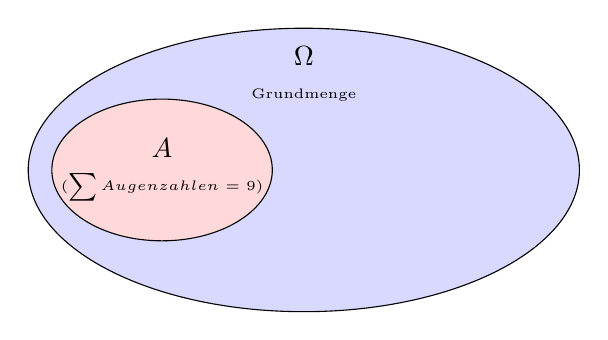
\begin{tikzpicture}
            {
    \def\ninecircle{(-1.8,0) ellipse (1.4cm and 0.9cm)}
    \def\omegacircle{(0,0) ellipse (3.5cm and 1.8cm)}

    \fill[blue!15] \omegacircle;
    \fill[red!15] \ninecircle;

    \draw \omegacircle node[above=0.75cm, text width=2.8cm,align=center] {$\Omega$\\\tiny{Grundmenge}};
    \draw \ninecircle node[text width=2.8cm,align=center] {$A$\\\tiny{($\sum\text{Augenzahlen}=9$)}};
}

        \end{tikzpicture}
        \label{fig:teilmenge1}
    }
    \subfigure[Teilmenge $A\subset \Omega$ und Teilmenge $B\subset \Omega$]{
        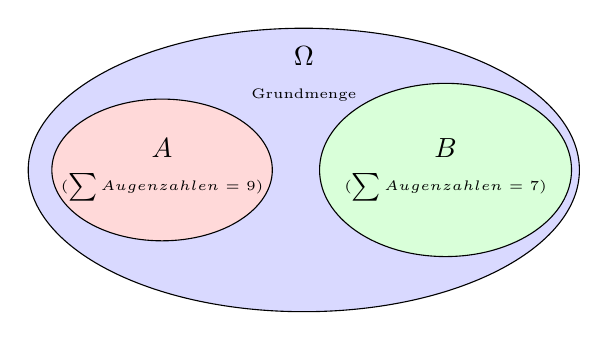
\begin{tikzpicture}
            {
    \def\ninecircle{(-1.8,0) ellipse (1.4cm and 0.9cm)}
    \def\sevencircle{(+1.8,0) ellipse (1.6cm and 1.1cm)}
    \def\omegacircle{(0,0) ellipse (3.5cm and 1.8cm)}

    \fill[blue!15] \omegacircle;
    \fill[red!15] \ninecircle;
    \fill[green!15] \sevencircle;

    \draw \omegacircle node[above=0.75cm, text width=2.8cm,align=center] {$\Omega$\\\tiny{Grundmenge}};
    \draw \ninecircle node[text width=2.8cm,align=center] {$A$\\\tiny{($\sum\text{Augenzahlen}=9$)}};
    \draw \sevencircle node[text width=2.8cm,align=center] {$B$\\\tiny{($\sum\text{Augenzahlen}=7$)}};
}

        \end{tikzpicture}
        \label{fig:teilmenge2}
    }
    \label{fig:teilmengen}
    \caption{Teilmengen der Grundmenge $\Omega$}
    \end{figure}

    Wir arbeiten also mit Mengen, die eine bestimmte Wahrscheinlichkeit
    besitzen. Im besten Fall enthält die Menge alle Elemente, im
    schlechtesten Fall keine. Es gilt:
    \begin{equation*}
        0\le \mathbb{P}\left(A\right)\le 1
    \end{equation*}
    Zusätzlich geben wir uns auch zufrieden, wenn die Summe der Augenzahlen 7 ergibt. (siehe Abbildung \ref{fig:teilmenge2})

    \begin{equation*}
        B=\{\left(1,6\right),\left(2,5\right),\left(3,4\right),\left(4,3\right),\left(5,2\right),\left(6,1\right)\}
    \end{equation*}

    Diese Mengen sind \textbf{disjunkt}\index{disjunkte Mengen}, besitzen also keine gleichen Elemente. Die
    Wahrscheinlichkeit, dass $A$ oder $B$ eintrifft, kann durch die einfache
    Addition der einzelnen Wahrscheinlichkeiten berechnet werden:

    \begin{equation*}
        \mathbb{P}(A\cup B)=\mathbb{P}\left(A\right)+\mathbb{P}\left(B\right)
    \end{equation*}
    \begin{equation*}
        0\le \mathbb{P}\left(A\right)\le \mathbb{P}\left(B\right)\le \mathbb{P}\left(A+B\right)\le 1
    \end{equation*}
    \begin{definition}[$\sigma$-Algebra]\index{sigma-Algebra@$\sigma$-Algebra}:

        Da wir später öfters noch den Begriff  $\sigma$-Algebra brauchen werden, möchte ich
        sie zuerst allgemein definieren. Diese Algebra kommt aus der
        Mengenlehre und besitzt drei wichtige Eigenschaften:

        \begin{itemize}
            \item $\Omega \in \mathcal S$
            \item Ist $A\in \mathcal S$ dann ist auch $A^{C}\in \mathcal S$
            \item Sind $A_{i}\in \mathcal S,\,i\in \mathbb{N}$, so ist auch $\cup _{i=1}^{{\infty}}A_{i}\in \mathcal S$
        \end{itemize}
    \end{definition}
    Angenommen wir werfen eine Münze. Dann ist die Grundmenge $\Omega$ 
    (manchmal auch \textbf{Obermenge}\index{Obermenge} bezeichnet):
    \begin{equation*}
        \Omega =\{K,Z\}
    \end{equation*}

    und die Elementarereignisse $\{K\}$ und $\{Z\}$ Nur was ist jetzt $\mathcal S$? Ohne
    weitere Angaben gilt:

    \begin{equation*}
        \mathcal S=\{\emptyset,\{K\},\{Z\},\{K,Z\}\}
    \end{equation*}


    \begin{bsp}\label{bsp:wuerfel}
        Angenommen wir werfen einen Würfel:
        \begin{equation*}
            \Omega=\{1,2,3,4,5,6\}
        \end{equation*}
        und die Elementarereignisse $\{1\},\{2\},...,\{6\},$. Ohne weitere Einschränkungen gilt
        \[\mathcal S=\{\emptyset,\{1\},...,\{1,2\},...,\{2,4,5\},...,\{1,2,5,6\},...,\{1,2,3,4,6\},...,\{1,2,3,4,5,6\}\}\]

        $\mathcal S$ muss jedoch nicht immer die gesamte Potenzmenge sein. Möchten wir nur folgenden Fälle betrachten:
        \begin{eqnarray*}
            A &=& \{2,4,6\}=\text{Gerade Zahl wird geworfen}\\
            B &=& \{1,3,5\}=\text{Ungerade Zahl wird geworfen}\\
        C &=& \{6\}
        \end{eqnarray*}
        Diese Algebra besteht aus $2^3$ Elementen:
        \begin{equation*}
            \mathcal S=\{\emptyset,\{6\},\{2,4,6\},\{1,3,5\},\{1,3,5,6\},\{1,2,3,4,5\},\{1,2,3,4,5,6\}\}
        \end{equation*}
        Die einzelnen Elemente lassen sich direkt aus den Eigenschaften einer $\sigma$-Algebra erstellen.
    \end{bsp}
    
    Mit diesem Wissen können wir uns nun den Axiomen von Kolmogorov zuwenden.

    \begin{definition}[Axiome von Kolmogorov]\label{def:axiome_kolmogorov}:
        \index{Axiome von Kolmogorov}
        Ist  $\Omega$ eine Grundmenge und $\mathcal S$ eine $\sigma$-Algebra von $\Omega$. Eine Abbildung
        \begin{equation*}
            \mathbb{P}:\mathcal S\rightarrow \mathbb{R}
        \end{equation*}
        heißt \textbf{Wahrscheinlichkeit}\index{Wahrscheinlichkeit} oder \textbf{Wahrscheinlichkeitsmaß}\index{Wahrscheinlichkeitsmaß}, wenn $\mathbb{P}$ die folgenden drei Eigenschaften besitzt:

        \begin{enumerate}
            \item Wahrscheinlichkeit einer beliebigen Menge zwischen 0 und 1:\\
                $\forall A\in \mathcal S: 0\leq\mathbb{P}(A)\leq 1$
            \item Wahrscheinlichkeit der leeren Menge ist 0:\\
                $\mathbb P\left({\emptyset}\right)=0$
            \item Ergebnis ist immer in der Grundmenge:\\ 
                $\mathbb P\left(\Omega \right)=1$
            \item Addition von disjunkten Mengen:\\
                Wenn $A_{n},n\in\mathbb{N}$ disjunkte Mengen sind, dann gilt:
                \[\mathbb{P}\left(\bigcup_{n\in\mathbb{N}}A_n\right)=\sum_{n\in\mathbb{N}}\mathbb{P}(A_n)\]
        \end{enumerate}
        Das Tripel $(\Omega, \mathcal S, \mathbb{P})$ heißt \textbf{Wahrscheinlichkeitsraum}\index{Wahrscheinlichkeitsraum}.
    \end{definition}

    Bei unserem Würfelspiel (siehe Beispiel \ref{bsp:wuerfel}) mit den zwei geworfenen Würfeln können wir noch
    weitere Eigenschaften feststellen. Einerseits gibt es endlich viele
    mögliche Ausgänge ($|\Omega|<{\infty}$), andererseits
    besitzt jede Kombination $k$ die gleiche Wahrscheinlichkeit (${|\Omega|=36\Rightarrow}$\\
    ${\mathbb{P}\left(k\right)=\frac{1}{|\Omega|}=\frac{1}{36}}$) und
    schlussendlich schließen sich die Ereignisse aus. In Tabelle \ref{tab:wuerfeln} sieht man alle möglichen Kombinationen sowie jede Einzelwahrscheinlichkeit.

\begin{table}
    \centering
    \begin{tabular}{|c|c|c|c|c|c|c|}
        \hline
        \diagbox{Würfel 1}{Würfel 2} & 1 & 2 & 3 & 4 & 5 & 6\\
        \hline
        1 & $\frac{1}{16}$ & $\frac{1}{16}$ & $\frac{1}{16}$ & $\frac{1}{16}$ & $\frac{1}{16}$ & $\frac{1}{16}$\\
        \hline
        2 & $\frac{1}{16}$ & $\frac{1}{16}$ & $\frac{1}{16}$ & $\frac{1}{16}$ & $\frac{1}{16}$ & $\frac{1}{16}$\\
        \hline
        3 & $\frac{1}{16}$ & $\frac{1}{16}$ & $\frac{1}{16}$ & $\frac{1}{16}$ & $\frac{1}{16}$ & $\frac{1}{16}$\\
        \hline
        4 & $\frac{1}{16}$ & $\frac{1}{16}$ & $\frac{1}{16}$ & $\frac{1}{16}$ & $\frac{1}{16}$ & $\frac{1}{16}$\\
        \hline
        5 & $\frac{1}{16}$ & $\frac{1}{16}$ & $\frac{1}{16}$ & $\frac{1}{16}$ & $\frac{1}{16}$ & $\frac{1}{16}$\\
        \hline
        6 & $\frac{1}{16}$ & $\frac{1}{16}$ & $\frac{1}{16}$ & $\frac{1}{16}$ & $\frac{1}{16}$ & $\frac{1}{16}$\\
        \hline
    \end{tabular}
    \caption{Würfelergenisse und Wahrscheinlichkeiten mit 2 Würfeln (Beispiel \ref{bsp:wuerfel})}\label{tab:wuerfeln}
\end{table}

    Das führt uns zur Definition eines Laplace-Experiments:
    \begin{definition}[Laplace-Experiment]\index{Laplacescher Wahrscheinlichkeitsraum}\index{Laplace-Experiment|see{Laplacescher Wahrscheinlichkeitsraum}}:\\
        Im Laplace-Experiment mit endlich vielen Ausgängen besitzt jeder Ausgang
        die gleiche Wahrscheinlichkeit.
        \begin{equation*}
            \mathbb{P}(A)=\frac{|A|}{|M|}
        \end{equation*}
    \end{definition}

    \begin{definition}[Weitere Eigenschaften aus den Axiomen von Kolmogorov]:\\
        \index{Axiome von Kolmogorov!weitere Eigenschaften}
        \begin{enumerate}
            \item Wahrscheinlichkeit, dass $A$ nicht auftritt:\\
                $\mathbb{P}\left(A^{C}\right)=1-\mathbb{P}(A)$
            \item $A$ ist eine Teilmenge von $B$ ($A\subseteq B)$\\
                Wenn $A\subseteq B$, dann gilt: $\mathbb{P}(A)\le \mathbb{P}(B)$
            \item Vereinigung von $A$ und $B$:\\
                $\mathbb{P}(A\cup B)=\mathbb{P}(A)+\mathbb{P}(B)-\mathbb{P}(A\cap B)$
            \item Vereinigung ist kleiner, gleich der Summe
                \[\text{Für }A_n\subseteq A_{n+1}:\;\;\mathbb{P}\left(\bigcup_nA_n\right)=\lim_n\mathbb{P}(A_n)\]
                \[\text{Für }A_n\subseteq A_{n+1}:\;\;\mathbb{P}\left(\bigcup_nA_n\right)\leq\sum_n\mathbb{P}(A_n)\]
        \end{enumerate}
    \end{definition}

    \textbf{Additionstheorem}\\
    Als Anwendung des Satzes \ref{satz:additionstheorem} berechnen wir die Wahrscheinlichkeit, dass
    eine zufällig gewählte Permutation von $n$ Elementen keinen Fixpunkt hat.
    Das Additionstheorem scheint auf den ersten Blick etwas kompliziert zu
    sein, ist aber ein einfaches Schema, das nur wiederholt werden muss.

    \begin{satz} \textbf{Additionstheorem}\index{Additionstheorem}\index{Siebformel}
    \label{satz:additionstheorem}
    \[\mathbb{P}\left(\bigcup_{i=1}^nA_i\right)=\sum_{i=1}^n(-1)^{i-1}S_i\]
    \[\text{mit } S_i=\sum_{i\leq j_1\leq j_2\leq ...\leq j_i\leq n} \mathbb{P}(A_{j_1}\cap...\cap A_{j_i})\]
    Also somit:
    \[\mathbb{P}(\bigcup_i A_i)=\sum_i\mathbb{P}(A_i)-\sum_{i<j}\mathbb{P}(A_i\cap A_j)+\sum_{i<j<k}\mathbb{P}(A_i\cap A_j\cap A_k)-+...\]
    \end{satz}

    Vorher haben wir gesagt, dass zwei disjunkte Mengen
    einfach addiert werden können. Sind diese jedoch nicht vollständig
    disjunkt, es existieren also Elemente, die in beiden Mengen enthalten
    sind, so würden manche Elemente mehrmals gezählt werden. Das Beispiel \ref{bsp:ehepaare_tanzen} 
    verdeutlicht dieses Problem genauer.

    \textbf{Formale Berechnung: Wahrscheinlichkeit, dass kein Fixpunkt existiert}

    Im Beispiel \ref{bsp:ehepaare_tanzen} ist ein Fixpunkt ein Ehepaar, das nach dem
    Signal zusammen bleibt. Wir benutzen in solchen Beispielen die
    Gegenwahrscheinlichkeit, betrachten den Fall, dass mindestens ein
    Fixpunkt $A$ existiert.

    Vereinigung aller Wahrscheinlichkeiten, dass ein Fixpunkt existiert: 

    \begin{equation*}
        \mathbb{P}\left(A\right)=\mathbb{P}\left(\overset{n}{\underset{i=1}{{\bigcup}}}A_{i}\right)=\sum
    _{i=1}^{n}\left(-1\right)^{i-1}S_{i}
    \end{equation*}

    Dafür müssen wir die Summanden $S_{k}$ berechnen. Das Ereignis $A_{1}\cap ... \cap A_{k}$ tritt ein, wenn
    $j_1,...,j_n$ Fixpunkte sind, die anderen $n-k$ Elemente können beliebig vertauscht werden. Es gibt $(n-k)!$
    Möglichkeiten, diese anzuordnen. Insgesamt existieren $n!$ Möglichkeiten, die Wahrscheinlichkeit ist also
    $\frac{(n-k)!}{n!}$. Außerdem existieren $\binom{n}{k}$ Möglichkeiten, aus $n$ Paaren, $k$ auszuwählen. 
    Wir schreiben für $S_{k}$:

    \[S_{k}=\binom{n}{k}\frac{(n-k)!}{n!}=\frac{1}{k!}\]

    Somit können wir $\mathbb P\left(A\right)$ und die eigentlich wichtigere Wahrscheinlichkeit 
    $\mathbb P\left(A^C\right)$ berechnen:

    \[
    \mathbb P\left(A\right)=\sum_{k=1}^{n}\left(-1\right)^{k-1}\frac{1}{k!}\Rightarrow
    \mathbb P\left(A^{C}\right)=1-\mathbb{P}\left(A\right)=\sum_{k=0}^{n}{\left(-1\right)^{k}\frac{1}{k!}}
    \]
    Die Umformung kann überprüft werden,
    indem die ersten paar Summanden aufgeschrieben werden. Für große $n$ konvergiert die Reihe gegen
    $\frac{1}{e}$.
    Die Näherung ist so gut, dass sich die Anzahl der Permutationen ohne
    Fixpunkt (für $n\ge1$) bestimmen lässt, indem man $\frac{n!}{e}$
    auf die nächste ganze Zahl rundet.
    \newpage
    \begin{bsp}[Ehepaare tanzen (Additionstheorem)]\label{bsp:ehepaare_tanzen}

    Nun stellen wir uns folgende Situation vor: Drei Ehepaare tanzen
    zusammen. Nach einer Weile ertönt ein Signal, die Namen aller Männer
    werden in ein Topf geworfen und jede Frau darf sich einen Namen ziehen.
    Nun stellt sich uns die Frage, wie hoch die Wahrscheinlichkeit ist,
    dass kein Ehepaar miteinander tanzt.

    Dafür benutzen wir die Gegenwahrscheinlichkeit, $\mathbb P\left(\text{kein Ehepaar tanzt}\right)$ ergibt sich durch 
    $1-\mathbb P\left(\text{mind. ein Ehepaar tanzt}\right)$.

    \textbf{Ich definiere:}
    \[\mathbb P\left(E_{i}\right)=\text{Ehepaar $i$ tanzt nach dem Signal weiterhin miteinander}\]

    Der schwarze Rahmen in Abbildung \ref{fig:tanzen1} steht für alle
    Ausgangsmöglichkeiten nach dem Signal, er ist die Grundmenge $\Omega$. Darin
    befinden sich drei Kreise, jeder Kreis beinhaltet die
    Wahrscheinlichkeit, dass das entsprechende Ehepaar weiterhin
    miteinander tanzt.

    Wie bereits erwähnt, benutzen wir die Gegenwahrscheinlichkeit. Dafür
    müssen wir die orange Fläche in Abbildung \ref{fig:tanzen2} berechnen.

    Instinktiv würden wir jetzt folgende Gleichung aufschreiben:

    \[
        1-\mathbb{P}\left(\text{min. ein Ehepaar tanzt}\right)=1-\mathbb{P}(E_1)+\mathbb{P}(E_2)+\mathbb{P}(E_3)
    \]
    Jedoch wurden einige Flächenelemente doppelt gezählt. Diese sind in Abbildung \ref{fig:tanzen3} orange gekennzeichnet:

    Damit unsere Gleichung wieder stimmt, müssen wir diese abziehen:

    \begin{eqnarray*}
         &1-\mathbb{P}\left(\text{min. ein Ehepaar tanzt}\right)=\\
         &=1-\mathbb{P}(E_1)+\mathbb{P}(E_2)+\mathbb{P}(E_3)-\mathbb{P}(E_1\cap E_2)-\mathbb{P}(E_1\cap E_3)-\mathbb{P}(E_2\cap E_3)
    \end{eqnarray*}
    Nun fehlt uns nur noch eine kleine Korrektur, denn durch den letzten
    Schritt haben wir das kleine Mittelstück einmal zu viel abgezogen.

    \begin{eqnarray*}
         &1-\mathbb{P}\left(\text{min. ein Ehepaar tanzt}\right)=\\
         &=1-\mathbb{P}(E_1)+\mathbb{P}(E_2)+\mathbb{P}(E_3)-\mathbb{P}(E_1\cap E_2)-\mathbb{P}(E_1\cap E_3)\\
         &-\mathbb{P}(E_2\cap E_3)+\mathbb{P}(E_1\cap E_2\cap E_3)
    \end{eqnarray*}
	\end{bsp}

    \begin{figure}
    \centering
    \subfigure[Ehepaare $E_1-E_3$ als Teilmengen von $\Omega$]{
        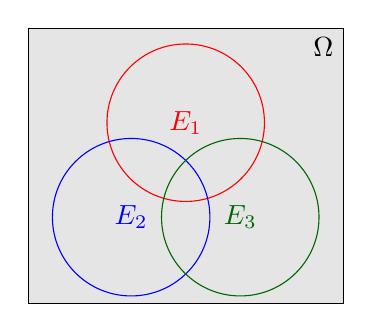
\begin{tikzpicture}
            {
    \def\firstcircle{(90:0.8cm) circle (1cm)}
    \def\secondcircle{(210:0.8cm) circle (1cm)}
    \def\thirdcircle{(330:0.8cm) circle (1cm)}
    \def\rectangle{(-2,-1.5) rectangle (2,2)}

    \fill[black!10] \rectangle;

    \draw[red] \firstcircle node {$E_1$};
    \draw[blue] \secondcircle node {$E_2$};
    \draw[green!40!black] \thirdcircle node {$E_3$};
    \draw[black] \rectangle node[below left,black] {$\Omega$};
}

        \end{tikzpicture}
        \label{fig:tanzen1}
    }
    \subfigure[Fläche, die für Gegenwahrscheinlichkeit berechnet werden soll]{
        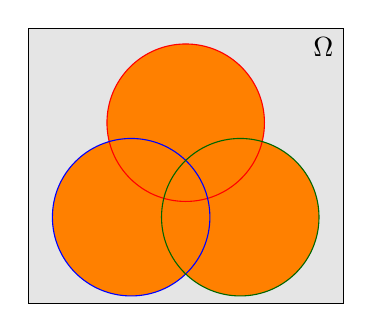
\begin{tikzpicture}
            {
    \def\firstcircle{(90:0.8cm) circle (1cm)}
    \def\secondcircle{(210:0.8cm) circle (1cm)}
    \def\thirdcircle{(330:0.8cm) circle (1cm)}
    \def\rectangle{(-2,-1.5) rectangle (2,2)}

    \fill[black!10] \rectangle;
    \fill[orange] \firstcircle;
    \fill[orange] \secondcircle;
    \fill[orange] \thirdcircle;

    \draw[red] \firstcircle;
    \draw[blue] \secondcircle;
    \draw[green!40!black] \thirdcircle;
    \draw[black] \rectangle node[below left,black] {$\Omega$};
}

        \end{tikzpicture}
        \label{fig:tanzen2}
    }
    \subfigure[Fläche, die doppelt gezählt wurde]{
        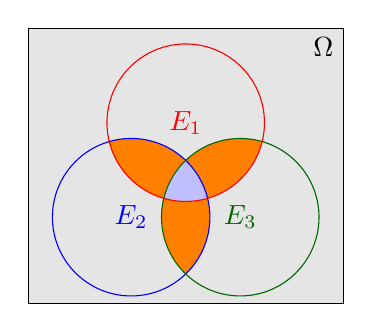
\begin{tikzpicture}
            {
    \def\firstcircle{(90:0.8cm) circle (1cm)}
    \def\secondcircle{(210:0.8cm) circle (1cm)}
    \def\thirdcircle{(330:0.8cm) circle (1cm)}
    \def\rectangle{(-2,-1.5) rectangle (2,2)}

    \fill[black!10] \rectangle;
    \fill[black!10] \firstcircle;
    \fill[black!10] \secondcircle;
    \fill[black!10] \thirdcircle;

    \begin{scope}
        \clip \firstcircle;
        \fill[orange] \secondcircle;
    \end{scope}
    \begin{scope}
        \clip \firstcircle;
        \fill[orange] \thirdcircle;
    \end{scope}
    \begin{scope}
        \clip \secondcircle;
        \fill[orange] \thirdcircle;
    \end{scope}

    \begin{scope}
        \clip \firstcircle;
        \clip \secondcircle;
        \fill[blue!25] \thirdcircle;
    \end{scope}

    \draw[red] \firstcircle node {$E_1$};
    \draw[blue] \secondcircle node {$E_2$};
    \draw[green!40!black] \thirdcircle node {$E_3$};
    \draw[black] \rectangle node[below left,black] {$\Omega$};
}

        \end{tikzpicture}
        \label{fig:tanzen3}
    }
    \label{fig:teilmengen}
    \caption{Der Kreis $E_1$ gibt z.B. die Wahrscheinlichkeit an, dass das Ehepaar $E_1$ nach dem Ziehen wieder miteinander Tanzt. Zu Beispiel \ref{bsp:ehepaare_tanzen}}
    \end{figure}
    \index{Axiome von Kolmogorov|)}



	\newpage
    \section{Bedingte Wahrscheinlichkeiten}\index{Bedingte Wahrscheinlichkeit|(}\index{Wahrscheinlichkeit!Bedingte -|see{Bedingte Wahrscheinlichkeit}}

    \begin{definition}\textbf{Die Bedingte Wahrscheinlichkeit}
    \label{def:bedingte_wahrscheinlichkeit}

    Sie gibt an, wie wahrscheinlich ein Ereignis
    ist, wenn ein anderes Ereignis schon eingetreten ist.

    \[
        \underbrace{\mathbb{P}(A|B)}_{\shortstack{\text{Wahrscheinlichkeit von $A$}\\\text{ unter der Bedingung $B$}}}=
        \frac{\overbrace{\mathbb P(A\cap B)}^{\shortstack{\text{Wahrscheinlichkeit, dass $A$}\\\text{und $B$ gleichzeitig eintreten.}}}}
        {\underbrace{\mathbb{P}(B)}_{\shortstack{\text{Wahrscheinlichkeit,}\\\text{dass $B$ eintritt}}}}
    \]
    \end{definition}

    Diese Formel lässt sich am besten graphisch veranschaulichen. Dafür
    unterscheiden wir zwei Fälle:
    \begin{multicols}{2}
        \textbf{Fall 1: disjunkte Mengen $A$, $B$}\\\index{disjunkte Mengen}
        Siehe Abbildung \ref{fig:disjunkt}
    \begin{equation*}
        \mathbb{P}\left(A|B\right)=\frac{\mathbb{P}\left(A\cap B\right)}{\mathbb{P}(B)}=\frac{0}{\mathbb{P}(B)}=0
    \end{equation*}
    Sobald wir wissen, dass $B$ eingetreten ist, können wir mit Sicherheit
    behaupten, dass $A$ nicht eingetreten ist.

    \columnbreak
        \textbf{Fall 2: nicht disjunk. Mengen $A$, $B$}\\ \index{disjunkte Mengen!nicht disjunkte Mengen}
        Siehe Abbildung \ref{fig:nicht_disjunkt}\\

        Nun wissen wir, dass $B$ eingetreten ist, unser Punkt liegt irgendwo in
        der blauen Fläche $\mathbb{P}(B)$.

    Die Wahrscheinlichkeit, dass nun auch
    die rote Fläche getroffen wurde, ist das Verhältnis der
    blauen zur grünen Fläche.

    Das wiederum ist
        \[\frac{\mathbb{P}(A\cap B)}{\mathbb{P}(B)}\]
    \end{multicols}

    \begin{figure}
    \centering
    \subfigure[$A$ und $B$ sind disjunkt]{
        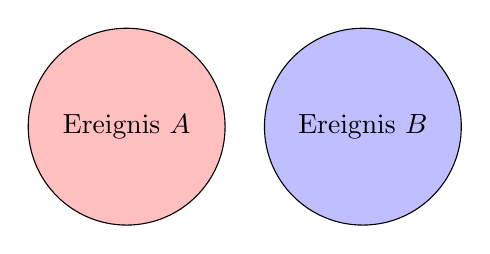
\begin{tikzpicture}
            {
    \def\firstcircle{(0,0) circle (1.25cm)}
    \def\secondcircle{(3,0) circle (1.25cm)}

    \fill[red!25] \firstcircle;
    \fill[blue!25] \secondcircle;

    \draw \firstcircle node {Ereignis $A$};
    \draw \secondcircle node {Ereignis $B$};
}

        \end{tikzpicture}
        \label{fig:disjunkt}
    }
    \subfigure[$A$ und $B$ sind nicht disjunkt]{
        \begin{tikzpicture}
            \input{chapters/wahrscheinlichkeitstheorie/nicht_disjunkt}
        \end{tikzpicture}
        \label{fig:nicht_disjunkt}
    }
    \label{fig:teilmengen}
    \caption{Disjunkte und nicht Disjunkte Mengen erklärt}
    \end{figure}

    \begin{satz}[Multiplikationssatz(Multiplikationstheorem)]\index{Multiplikationssatz}:
        \label{satz:multiplikationssatz}
        \index{Multiplikationstheorem|see{Multiplikationssatz}}\\
        Mit dem Multiplikationssatz wird die Wahrscheinlichkeit berechnet, dass
        die Ereignisse  $A_{1},A_{2},...,A_{k}$ gleichzeitig eintreten.

        Dafür drehen wir die Formel der bedingten Wahrscheinlichkeit um und
        erweitern sie:
        \[
            \mathbb{P}\left(A\cap B\right)=\mathbb{P}\left(B\right)\mathbb{P}(A|B)
        \]
    \end{satz}
    Die mehrfache Anwendung dieser Formel liefert:
    \[
        \mathbb{P}\left(A_{1}\cap ... \cap A_{k}\right)=
        \mathbb{P}\left(A_{1}\right)\mathbb{P}\left(A_{2}|A_{1}\right)\mathbb{P}\left(A_{3}|A_{1}\cap A_{2}\right) ... 
        \mathbb{P}\left(A_{k}|A_{1}\cap ... \cap A_{k-1}\right)
    \]

    \textbf{Die Ungleichung von Bonferroni kann das etwa Abschätzen.}\index{Ungleichung!von Bonferroni}\index{Bonferrroni Ungleichung|see{Ungleichung von Bonferroni}}
    \[\mathbb{P}(\bigcap_i A_i)=1-\sum_i\mathbb{P}(A_i^c)\]

    \begin{bsp}[Ziehen ohne Zurücklegen (Multiplikationstheorem)]:\\
    In einer Urne sind zwei schwarze und drei weiße Kugeln. Es wird dreimal
    ohne Zurücklegen gezogen und wir wollen die Wahrscheinlichkeit
    bestimmen, dass alle gezogenen Kugeln weiß sind. 

    Wir setzen also $A_{i}$ gleich dem Ereignis, dass die $i$-te gezogene Kugel weiß ist und suchen
    $\mathbb P(A_{1}\cap A_{2}\cap A_{3})$.

    \begin{tabular}{>{\centering\arraybackslash}p{0.28\linewidth}|>{\centering\arraybackslash}p{0.28\linewidth}|>{\centering\arraybackslash}p{0.28\linewidth}}
        &&\\
        \textbf{Zug 1} & \textbf{Zug 2} & \textbf{Zug 3} \\
            \trimbox{0 0 0 -0.4cm}{
                \begin{tikzpicture}
                    {
\begin{scope}[yshift=-180,yslant=0.5,xslant=-1]
    %circle circumventing the smallest cluster 
    \node[circle,circular glow,fill=red!20,draw=red,thick]
    at (4.4,2.8) {\phantom{perimetro}};
\end{scope}

%atom clusters are rotated for a better visualisation
\begin{scope}[rotate around = {-5:(0,0,0)}]
    \draw[-latex,thick](2,-4)node[below]
        {Ziehe} to[out=90,in=270] (2.3,-2.95);
    \foreach \x  in {6.6,7.1}
        \shadedraw [ball color=black] (\x,2.5,12.8) circle (0.25cm);
    \foreach \x  in {6.5,7,7.5}
        \shadedraw [ball color=white] (\x,2.5,13.5) circle (0.25cm);
\end{scope}
}
%Graphic
                \end{tikzpicture}
            } &
             \trimbox{0 0 0 -0.4cm}{
                \begin{tikzpicture}
                    \input{chapters/wahrscheinlichkeitstheorie/urne2}%Graphic
                \end{tikzpicture}
            } &
             \trimbox{0 0 0 -0.4cm}{
                \begin{tikzpicture}
                    \input{chapters/wahrscheinlichkeitstheorie/urne3}%Graphic
                \end{tikzpicture}
            } \\
            $\mathbb{P}(A_1)=\frac{3}{5}$ & $\mathbb{P}(A_2|A_1)=\frac{2}{4}=\frac{1}{2}$ &$\mathbb{P}(A_3|A_1\cap A_2)=\frac{1}{3}$\\
        &&\\
    \end{tabular}

    Nun wenden wir das Multiplikationstheorem an:
    \[
    \mathbb P\left(A_{1}\cap A_{2}\cap A_{3}\right)=
    \mathbb P\left(A_{1}\right)\mathbb P\left(A_{2}|A_{1}\right)\mathbb P\left(A_{3}|A_{1}\cap A_{2}\right)=
    \frac{3}{5}\cdot \frac{1}{2}\cdot \frac{1}{3}=\frac{1}{10}
    \]

    \end{bsp}

    \index{Bedingte Wahrscheinlichkeit|)}
    
    \section{Stochastische Unabhängigkeit}
    \index{Unabhängigkeit!stochastische|see{stochastische Unabhängigkeit}}
    \index{stochastische Unabhängigkeit|(}

    Zwei Ereignisse heißen stochastisch unabhängig, wenn gilt:

    \[
        \mathbb P\left(A\cap B\right)=
        \mathbb P\left(A\right)\cdot \mathbb P\left(B\right)\text{ bzw. }
        \mathbb P\left(A|B\right)=\mathbb P\left(A\right)=\mathbb P\left(A|B^{C}\right)
    \]
    Die Wahrscheinlichkeit des Eintretens von $A$ hängt nicht davon ab, ob das Ereignis $B$ oder $B^C$ eintritt.

    \begin{bsp} zur Erklärung: \\
        Sie erhalten 5{\texteuro}, falls
        ein geworfener Schwamm in der unteren Hälfte einer Tafel auftrifft,
        ansonsten verlieren Sie 5{\texteuro}. Sie stehen dabei in einem
        Nebenraum und sind sich noch nicht sicher, ob Sie die Wette annehmen 
        sollen. Bevor Sie die Wette platzieren, kommt ein {\quotedblbase}Freund{\textquotedblleft}
        und erzählt Ihnen, dass er für ein bisschen Geld verrät, 
        ob der Schwamm in der linken oder rechten Seite der Tafel gelandet ist.\\

        Was hilft Ihnen diese Information?\\

        Sein Angebot hilft ihnen nicht weiter, denn die neue Information ändert nichts
        an dem bisherigen Wissen über die Wette.
    \end{bsp}

    \begin{figure}
    \centering
    \subfigure[$A$ und $B$ sind disjunkt]{
        \begin{tikzpicture}
            {
    \def\firstrect{(-3,-1) rectangle (0,0.5)}
    \def\secondrect{(0,-1) rectangle (3,0.5)}
    \def\rectangle{(-3,-1) rectangle (3,0.5)}

    \fill[red!25] \secondrect;
    \fill[blue!25] \firstrect;

    \draw[black] \firstrect node[below left=0cm and 1.5cm] {\small{Ereig. $A$}};
    \draw[black] \secondrect node[below left] {\small{Ereig. $B$}};
    \draw[black] \rectangle;
}

        \end{tikzpicture}
        \label{fig:tafeln_disjunkt}
    }
    \subfigure[$A$ und $B$ sind nicht disjunkt]{
        \begin{tikzpicture}
            {
    \def\firstrect{(-3,-1) rectangle (1,0.5)}
    \def\secondrect{(-1,-1) rectangle (3,0.5)}
    \def\rectangle{(-3,-1) rectangle (3,0.5)}

    \fill[red!25] \secondrect;
    \fill[blue!25] \firstrect;

    \begin{scope}
        \clip \firstrect;
        \fill[orange] \secondrect;
    \end{scope}

    \draw[black] \firstrect node[below left=0cm and 2.5cm] {\small{Ereig. $A$}};
    \draw[black] \secondrect node[below left] {\small{Ereig. $B$}};
    \node[above] {$A\cap B$};
}

        \end{tikzpicture}
        \label{fig:tafeln_nicht_disjunkt}
    }
    \caption{Disjunkte und nicht disjunkte Tafeln}
    \label{fig:tafeln}
    \end{figure}

    Zur Verdeutlichung siehe Abbildung \ref{fig:tafeln}:
    Die Grundmenge $\Omega$ wird durch den Rahmen dargestellt, darin
    befinden sich die Mengen A und B (disjunkt und überlappend) Es gilt
    $\mathbb P\left(M\right)=1,\mathbb P\left(A\right)=0,5$
    und
    $\mathbb P\left(B\right)=0,5$.

    \begin{multicols}{2}
        Siehe Abbildung \ref{fig:tafeln_disjunkt}\\
        \begin{eqnarray*}
            \mathbb{P}(A\cap B) &=& \mathbb{P}(A)\cdot \mathbb{P}(B)\\
            0 &\neq& 0.25
        \end{eqnarray*}
    Wird $B$ getroffen, ist
    \[\mathbb{P}\left(A|B\right)=0\neq \mathbb P(A)\]
    
    Die Ereignisse sind stochastisch abhängig, dass $B$ getroffen wurde gibt
    uns viel Auskunft über die Wahrscheinlichkeit von $A$.
    
    \columnbreak
        Siehe Abbildung \ref{fig:tafeln_nicht_disjunkt}\\
        \begin{eqnarray*}
            \mathbb{P}(A\cap B) &=& \mathbb{P}(A)\cdot \mathbb{P}(B)\\
            0.25 &=& 0.25
        \end{eqnarray*}

    Wird $B$ getroffen, ist
    \[\mathbb P\left(A|B\right)=0.5=\mathbb P(A)\]

    Die Ereignisse sind stochastisch unabhängig, dass $B$ getroffen wurde,
    gibt uns keine Auskunft über die Wahrscheinlichkeit von $A$.
    \end{multicols}

    \begin{definition}\textbf{Totale Unabhängigkeit}\index{Unabhängigkeit!Totale-|see{Totale Unabhängigkeit}}\index{Totale Unabhängigkeit}\\
        Die $n$ Ereignisse $A_{1},A_{2},...,A_{n}$ heißen total unabhängig, falls für jede Auswahl $A_{1},...,A_{k}$ 
        von $k$ Ereignissen gilt:

        \[
            \mathbb P\left(A_{1}\cap A_{2}\cap ... \cap A_{k}\right)=
            \mathbb P\left(A_{1}\right)\mathbb P\left(A_{2}\right)... \mathbb P(A_{k})
        \]

    \end{definition}

    \begin{definition}\textbf{Paarweise Unabhängigkeit}\index{Unabhängigkeit!Paarweise-|see{Paarweise Unabhängigkeit}}\index{Paarweise Unabhängigkeit}\\
        Die $n$ Ereignisse $A_{1},A_{2},...,A_{n}$ heißen paarweise unabhängig, wenn für alle $1\leq i<j\leq n$ gilt:

        \[
            \mathbb P\left(A_{i}\cap A_{j}\right)=
            \mathbb P\left(A_{i}\right)\mathbb P\left(A_{j}\right)
        \]

    \end{definition}

    \begin{bsp}[aus Wikipedia\cite{wiki:001}]:\\
        In einer Schachtel befinden sich 4 Zettel mit folgenden Zahlenkombinationen: 112, 121, 211, 222. Einer der Zettel wird zufällig (je mit Wahrscheinlichkeit 1/4) gezogen. Wir betrachten dann folgende drei Ereignisse:

            \[A_{1}=\lbrace 1\ {\mathrm {an\ erster\ Stelle}}\rbrace mit \mathbb P(A_{1})={\frac {1}{2}}\]
            \[A_{2}=\lbrace 1\ {\mathrm {an\ zweiter\ Stelle}}\rbrace mit \mathbb P(A_{2})={\frac {1}{2}}\]
            \[A_{3}=\lbrace 1\ {\mathrm {an\ dritter\ Stelle}}\rbrace mit \mathbb P(A_{3})={\frac {1}{2}}\]

        Offensichtlich sind die drei Ereignisse paarweise unabhängig, da gilt

            \[\mathbb P(A_{1}\cap A_{2})=P(A_{1})\cdot \mathbb P(A_{2})={\frac {1}{4}}\]
            \[\mathbb P(A_{1}\cap A_{3})=P(A_{1})\cdot \mathbb P(A_{3})={\frac {1}{4}}\]
            \[\mathbb P(A_{2}\cap A_{3})=P(A_{2})\cdot \mathbb P(A_{3})={\frac {1}{4}}\]

        Die drei Ereignisse sind jedoch nicht (gemeinsam) unabhängig, da gilt

            \[\mathbb P(A_{1}\cap A_{2}\cap A_{3})=0\neq {\frac {1}{8}}=\mathbb P(A_{1})\cdot \mathbb P(A_{2})\cdot \mathbb P(A_{3})\]

        Des Weiteren kann aus $\mathbb P(A_{1}\cap A_{2}\cap A_{3})=\mathbb P(A_{1})\cdot \mathbb P(A_{2})\cdot \mathbb P(A_{3})$ nicht geschlossen werden, dass die drei Ereignisse paarweise unabhängig sind.

    \end{bsp}


    \begin{satz}[von der vollständigen Wahrscheinlichkeit]:\index{Wahrscheinlichkeit!Vollständige-|see{Vollständige Wahrscheinlichkeit}}\index{Vollständige Wahrscheinlichkeit}\index{Totale Wahrscheinlichkeit|see{Vollständige Wahrscheinlichkeit}}\\
    Für den Satz der Vollständigen bzw. totalen Wahrscheinlichkeit brauchen wir folgende Bedingungen:
    \label{satz:vollstaendige_wahrscheinlichkeit}

    \begin{itemize}
        \item Disjunkte Ereignismengen $B_{i}$ von denen $\mathbb P\left(B_{i}\right)$ bekannt ist
        \item $\mathbb P\left(A|B_{i}\right)$ muss bekannt bzw. leicht berechenbar sein
        \item $\sum_{i}{\mathbb P\left(B_{i}\right)}=1$, somit wird die gesamte Grundmenge auf $i$ Flächen aufgeteilt.
    \end{itemize}

    Wir möchten uns also die vollständige Wahrscheinlichkeit berechnen, dass
    $A$ eintrifft. Unser Problem liegt darin, dass wir nur wissen, wie sicher
    $A$ eintrifft, wenn bereits ein anderes Ereignis
    $B_{i}$ eingetroffen ist (bedingte Wahrscheinlichkeit!). Somit ergibt sich:
    \[
        \mathbb P\left(A\right)=\sum _{i}{\mathbb P(B_{i})\mathbb P\left(A|B_{i}\right)}
    \]
    \end{satz}

    \begin{satz}[von Bayes]:\index{Satz von Bayes}\index{Bayes!Satz|see{Satz von Bayes}}\\
        \label{satz:bayes}
        \[\mathbb{P}(A|B)\;\;\Longleftrightarrow\;\;\mathbb{P}(B|A)\]

        Ist die bedingte Wahrscheinlichkeit von $B$ unter $A$, also 
        $\mathbb P\left(B|A\right)$ bekannt, kann mit dem Satz von Bayes
        die Wahrscheinlichkeit von $A$ unter B, also $\mathbb P(A|B)$
        berechnet werden. 
        
        Dafür definieren wir die bedingte Wahrscheinlichkeit
        für beide Fälle, stellen um und erhalten:

        \begin{eqnarray*}
            \mathbb P\left(A|B\right)&=&\frac{\mathbb P\left(B\cap
                A\right)}{\mathbb P\left(B\right)}\Rightarrow \mathbb P\left(B\cap
                A\right)=\mathbb P\left(B\right)\mathbb P(A|B)\\
            \mathbb P\left(B|A\right)&=&\frac{\mathbb P\left(B\cap
                A\right)}{\mathbb P(A)}\Rightarrow \mathbb P\left(B\cap
                A\right)=\mathbb P\left(A\right)\mathbb P(B|A)\\
            \mathbb P\left(B\right)\mathbb P\left(A|B\right)&=&\mathbb P\left(B\cap A\right)=
                \mathbb P\left(A\right)\mathbb P\left(B|A\right)\\
        \end{eqnarray*}
        Somit erhalten wir:
        \[\mathbb P\left(A|B\right)=\frac{\mathbb P\left(B|A\right)\mathbb P\left(A\right)}{\mathbb P(B)}\]
    \end{satz}

    \begin{bsp}\label{bsp:krankheit} \textbf{Krankheit (Vollständige Wahrscheinlichkeit \& Satz von Bayes)}\\

    Von einer Krankheit sind 2\% der Bevölkerung betroffen. Ein Test gibt
    bei einem Kranken mit Wahrscheinlichkeit 0.99 ein positives Ergebnis,
    bei einem Gesunden mit Wahrscheinlichkeit 0.01.

    \begin{enumerate}[a)]
        \item \label{itm:krankheit_a}Bestimmen Sie die Wahrscheinlichkeit, dass eine zufällig gewählte
            Person positiv getestet wird.

            Abbildung \ref{fig:krankheit} beschreibt die Situation. Der grüne Rahmen kennzeichnet den
            Wahrscheinlichkeitsbereich für ein positives Testergebnis. Es ist klar
            ersichtlich, dass die Trefferquote bei kranken Personen viel höher ist,
            als bei gesunden. Nun möchten wir die Wahrscheinlichkeit bestimmen,
            dass eine zufällig gewählte Person positiv getestet ist, also im
            grün-strichlierten Bereich liegt.

            \[\mathbb P\left(A\right)=\text{Positiv getestet}\]
            \[\mathbb P\left(B\right)=\text{Person gesund}\]
            \[\mathbb P\left(A\right)=\mathbb P\left(B\right)\mathbb P\left(A|B\right)+\mathbb P\left(B^{C}\right)\mathbb P\left(A|B^{C}\right) = 0.98\cdot 0.01+0.02\cdot 0.99=0.0296\approx 3\%\]
            Hier wurde $\mathbb P(A)$ mit dem Satz der Vollständigen Wahrscheinlichkeit berechnet. 
        \item Bestimmen Sie die bedingte Wahrscheinlichkeit dafür, dass eine
            zufällig gewählte Person krank ist, wenn das Testergebnis positiv ist.

            Mit dem Wissen aus \ref{itm:krankheit_a}) kann nun  $P(B^{C}|A)$ berechnet werden.

            \[
                \mathbb P(B^{C}|A)=\frac{\mathbb P(B^{C}\cap A)}{\mathbb P\left(A\right)}=
                \frac{\mathbb P\left(B^{C}\right)\mathbb P(A|B^{C})}{\mathbb P(A)}=\frac{0.02\cdot 0.99}{0.0296}=0.6689\approx 67\%
            \]
            Hier wurde $\mathbb P\left(B^{C}\cap A\right)$ mit dem Satz von Bayes berechnet.
        \end{enumerate}
    \end{bsp}

    \begin{figure}
    \centering
        \begin{tikzpicture}
            {
    \def\firstrect{(-2,-2) rectangle (2,2)}
    \def\secondrect{(0.4,1.6) rectangle (2,2)}
    \def\thirdrect{(0.6,1.4) rectangle (2,2)}

    \fill[red!25] \secondrect;
    \fill[blue!25] \firstrect;

    \begin{scope}
        \clip \firstrect;
        \fill[orange] \secondrect;
    \end{scope}

    \draw[green,dashed,line width=2pt] \thirdrect;
    \draw[black] \firstrect node[below left=1.7 and 0.65] {\small{Gesund (98\%)}};
    \draw[black] \secondrect node[below left=-0.07 and -0.1] {\scriptsize{Krank (2\%)}};
}

        \end{tikzpicture}
        \caption{Krankheit in Bezug auf Testergebnis (grün Strichliert) siehe Beispiel \ref{bsp:krankheit}, (Achtung, übertrieben gezeichnet)}
        \label{fig:krankheit}
    \end{figure}

    \index{stochastische Unabhängigkeit|)}

    \index{Wahrscheinlichkeitstheorie|)}
}

{
    \chapter{Zufallsvariable}\index{Zufallsvariable|(}

    \section{Motivation und Einführung}\index{Zufallsvariable!Beschreibung|(}

    Bisher hat uns immer direkt das Ergebnis eines Elementarereignisses
    interessiert, zum Beispiel haben wir uns gefragt, wie wahrscheinlich es
    ist, dass eine Münze Kopf zeigt oder eine Drei gewürfelt wird. Nun
    interessiert uns aber nicht mehr das Elementarereignis, sondern die
    {\quotedblbase}Informationen{\textquotedblleft}, die aus mehreren
    Elementarereignissen entstehen. Am Einfachsten ist das mit einem
    Beispiel verständlich. 

    \begin{bsp}\label{bsp:muenze}
    Der Dozent bietet uns folgendes Spiel an: Jeder Student zahlt dem
    Dozenten 20 Cent Einsatz und wirft dann 3 Münzen. 
    
    Bei den Münzen wird
    {\quotedblbase}Kopf${\triangleq}K${\textquotedblleft} oder
    {\quotedblbase}Zahl${\triangleq}Z${\textquotedblleft} registriert. Je
    nach der Anzahl der geworfenen {\quotedblbase}Köpfe{\textquotedblleft}
    zahlt der Dozent anschließend die Beträge in Tabelle \ref{tab:auszahlungen}\\

    Wie wahrscheinlich sind die einzelnen Auszahlungen? Was muss der Dozent
    im Schnitt zahlen? Ist das Spiel fair? 
    
    Für die kürzere Schreibweise führen wir ein:

    \[X_{i}...\text{Anzahl der vom }i\text{-ten Studenten bei 3 Versuchen geworfene Köpfe}\]
    \[Y_{i}...\text{Auszahlung an den }i\text{-ten Studenten}\]

    Wir betrachten den ersten Studenten:

    Dieser wirft 2 {\quotedblbase}Köpfe{\textquotedblleft}, also ist $X_{1}=2$.

    Aber was heißt das und was ist der Unterschied zwischen $X_{1}$ und $X_{1}=2$?

    \begin{center}
    \begin{tabular}{c|c}
    \hline
    \textbf{Zufallsvariable} & \textbf{Realisation von $X_1$}\\
    \hline
     $X_1$ & $X_1=2$\\
     \parbox[t]{0.33\linewidth}{Symbolische Kurzbeschreibung des Münzspiels} 
            & \parbox[t]{0.33\linewidth}{Die Realisation $2$ ist eingetreten.}\\
     \hline
    \end{tabular}
    \end{center}

    Nun stellen wir uns natürlich die Frage, wie Wahrscheinlich der Student
    zweimal Kopf würfelt. Dafür betrachten wir zuerst die Grundmenge $\Omega$, also die Menge, die alle
    möglichen Ausgänge des Spiels beinhaltet:
    \[\Omega=\{ZZZ,KZZ,ZKZ,ZZK,KKZ,KZK,ZKK,KKK\}\]
    Wir gehen von einer fairen Münze aus, es gilt: $\mathbb P\left(Z\right)=\mathbb P\left(K\right)=\frac{1}{2}$.
    Zusätzlich wissen wir aus dem vorherigen Kapitel, dass wenn die
    Ereignisse total unabhängig sind, sich jede Wahrscheinlichkeit, zum Beispiel $\mathbb P\left(ZKZ\right)$,
    leicht berechnen lässt:
    \[\mathbb P\left(ZKZ\right)=\mathbb P(Z)\mathbb P\left(K\right)\mathbb P\left(Z\right)=\frac{1}{2}\cdot\frac{1}{2}\cdot\frac{1}{2}=\frac{1}{8}\]

    Das gilt trivialerweise auch für die anderen Ausgänge des Spiels. Und was macht die 
    Zufallsvariable $X_{1}$ genau? Sie {\quotedblbase}bewertet{\textquotedblleft} die 
    Elemente der Grundmenge $\Omega $ anhand der Anzahl von {\quotedblbase}Köpfen{\textquotedblleft}:
    \begin{eqnarray*}
        X_{1}\left(ZZZ\right)&=&0\\
        X_{1}\left(KZZ\right)=X_{1}\left(ZKZ\right)=X_{1}\left(ZZK\right)&=&1\\
        X_{1}\left(KKZ\right)=X_{1}\left(KZK\right)=X_{1}\left(ZKK\right)&=&2\\
        X_{1}\left(KKK\right)&=&3
    \end{eqnarray*}
    Mathematisch ausgedrückt ist eine Zufallsvariable eine Abbildung der Grundmenge $\Omega$ 
    in die reellen Zahlen:

    \[
    X_{1}:\Omega \rightarrow \mathbb R
    \]
    Diese Abbildung ist nicht bijektiv, wie sich mit Tabelle \ref{tab:zv_abbildungen} leicht nachprüfen lässt:\\

    Offensichtlich existieren jeweils drei Ereignisse, die auf 1 bzw. 2
    abbilden und somit ist die Abbildung nicht eindeutig umkehrbar.
    

    Anmerkung: für  $\mathbb P\left(X_{1}=1\right)$ bzw. $\mathbb P\left(X_{1}=2\right)$
    wurden die einzelnen Wahrscheinlichkeiten einfach addiert, da sich die Ereignisse paarweise
    ausschließen.
    \end{bsp}

    \begin{table}
        \centering
        \begin{tabular}{cc}
        \hline
        \textbf{Anzahl der Köpfe} & \textbf{Auszahlung in Cent}\\
        \hline
         0 & 0\\
         1 & 0\\
         2 & 20\\
         3 & 100\\
         \hline
        \end{tabular}
        \caption{Auszahlungsbeträge bei 3 Münzwürfen}\label{tab:auszahlungen}
    \end{table}

    \begin{table}
        \centering
        \begin{tabular}{ccc}
        \hline
        \textbf{Ereignisse} & \textbf{Realisationen von $X_1$}& \textbf{Wahrscheinlichkeit $P_1$}\\
        \hline
         $\{ZZZ\}$ & 0 & $\mathbb{P}(X_1=0)=\frac{1}{8}$\\
         $\{KZZ,ZKZ,KZZ\}$ & 1 & $\mathbb{P}(X_1=0)=\frac{3}{8}$\\
         $\{KKZ,KZK,ZKK\}$ & 2 & $\mathbb{P}(X_1=0)=\frac{3}{8}$\\
         $\{KKK\}$ & 3 & $\mathbb{P}(X_1=0)=\frac{1}{8}$\\
         \hline
        \end{tabular}
        \caption{Abbildungen der Ereignisse in Wahrscheinlichkeiten ($\Omega\to\mathbb R$)}\label{tab:zv_abbildungen}
    \end{table}
    \index{Zufallsvariable!Beschreibung|)}

    \section{Mathematische Definition}\index{Zufallsvariable!Mathematische Definition|(}

    Die Wahrscheinlichkeit des im vorherigen Kapitel (Siehe Definition \ref{def:axiome_kolmogorov}) beschrieben
    Wahrscheinlichkeitsraumes  $\left(\Omega,\mathcal S,\mathbb P\right)$ wird mithilfe von $X$ auf einen
    neuen Wahrscheinlichkeitsraum abgebildet.

    \[\left(\Omega ,\mathcal S,\mathbb P\right)\Rightarrow X\Rightarrow (\mathcal B,\mathcal F,\mathbb P_{X})\]
    Dem Ereignis $F\in \mathcal F$ ordnen wir nun die Wahrscheinlichkeit seiner {\quotedblbase}Verursacher{\textquotedblleft} zu:

    \[
    \mathbb P_{X}\left(F\right)=
    \mathbb P(X\in F)=\mathbb P\left(X^{-1}\left(F\right)\right)=
    \mathbb P\left(\{\omega:X\left(\omega \right)\in F\}\right)
    \]

    \begin{definition}
    Das \textbf{Wahrscheinlichkeitsmaß}\index{Wahrscheinlichkeitsmaß} $\mathbb P_{X}$ heißt das zu X gehörige \textbf{Bildmaß}.\index{Bildmaß}
    Vereinfacht kann $X$ auch als Abbildung 
    \[
    X:\Omega\rightarrow \mathbb R^{d}
    \]  
    definiert werden. Dabei gilt:

    \begin{itemize}
    \item wenn $\Omega$ überabzählbar ist, muss man von $X$ die Eigenschaft 
        \quotedblbase Messbarkeit\textquotedblleft verlangen.
    \item meistens ist $d=1$, bei $d>1$ wird $X=\left(X_{1},...,X_{d}\right)$ ein Vektor von reellen
        Zufallsvariablen.
    \end{itemize}
    \end{definition}

    \begin{bsp}\label{bsp:abbildung_wahrscheinlichkeitsraum} \textbf{anhand des Münzbeispiels (siehe Beispiel \ref{bsp:muenze})}\\
        \begin{itemize}
            \item $\Omega\;\Rightarrow\;\mathcal B$
                \[\{ZZZ,KZZ,ZKZ,ZZK,KKZ,KZK,ZKK,KKK\}\;\Rightarrow\;\{0,1,2,3\}\]
            \item $\mathcal S\;\Rightarrow\;\mathcal F$\\
                Abhängig von der Anforderung
            \item $\mathbb P\;\Rightarrow\;\mathbb P_X$
                \[\forall \omega \in \Omega :\mathbb P\left(\omega \right)=\frac{1}{8}\Rightarrow
                    \begin{cases}\mathbb P_{X_1}\left(0\right)=\mathbb P_{X_1}\left(3\right)=\frac{1}{8}\\
                    \mathbb P_{X_1}\left(1\right)=\mathbb P_{X_1}\left(2\right)=\frac{3}{8}
                    \end{cases}\]
        \end{itemize}

        \textbf{Graphische Erklärung}\\
        Alle Elementarereignisse  $\omega \in \Omega$, also
        die durch Zufall eingetretene Ereignisse (z.B. $\{ZZZ\},\{KZK\},\{KKK\}$),
        werden über die Abbildung der Zufallsvariable $X$ auf die reellen Zahlen
        und in die Menge $\mathcal B$
        abgebildet, dem Ereignis wird eine Realisation zugeordnet. 

        Abbildung \ref{fig:abbildung_wahrscheinlichkeitsraum} beschreibt das komplette System anschaulich: 
        
        Die blauen Bereiche repräsentieren eine Abbildung, die Quadrate einen
        vollständigen Wahrscheinlichkeitsbereich.

    \end{bsp}

    \begin{figure}
    \centering
        \includegraphics[width=5.8102in,height=7.8744in]{chapters/zufallsvariable/wahrscheinlichkeitsraum}
        \caption{Abbildung des Wahrscheinlichkeitsraumes von $X$ (siehe Beispiel \ref{bsp:abbildung_wahrscheinlichkeitsraum})}
        \label{fig:abbildung_wahrscheinlichkeitsraum}
    \end{figure}

    \index{Zufallsvariable!Mathematische Definition|)}
    \section{Diskrete Zufallsvariable}\index{Diskrete Zufallsvariable|(}\index{Zufallsvariable!diskret|see{Diskrete Zufallsvariable}}

    \begin{figure}
    \centering
        \begin{tikzpicture}
            {
    \begin{axis}[domain=0:8,
            axis x line=bottom, % no box around the plot, only x and y axis
            axis y line=left, % the * would suppress the arrow tips
            xlabel=Anzahl der Köpfe,
            ylabel=Wahrscheinlichkeit $p$,
            legend style={at={(1.05,0.75)}},
            xtick={0,1,...,4},
            %legend pos=south east,
            samples=50,
            height=6cm,
            width=10cm,
            clip=false]
            \def\pvala{0.125}
            \def\pvalb{0.375}
            \def\pvalc{0.375}
            \def\pvald{0.125}

            %calc missing values
            \pgfmathsetmacro{\tvala}{\pvala}
            \pgfmathsetmacro{\tvalb}{\pvala+\pvalb}
            \pgfmathsetmacro{\tvalc}{\pvala+\pvalb+\pvalc}
            \pgfmathsetmacro{\tvald}{\pvala+\pvalb+\pvalc+\pvald}

            \addplot[blue] coordinates{(-1,0)(0,0)};
            \addlegendentry[align=left]{Verteilungsfunktion};%TODO: add a better label
            \addplot[blue,forget plot] coordinates{(0,\tvala)(1,\tvala)};
            \addplot[blue,forget plot] coordinates{(1,\tvalb)(2,\tvalb)};
            \addplot[blue,forget plot] coordinates{(2,\tvalc)(3,\tvalc)};
            \addplot[blue,forget plot] coordinates{(3,1)(5,1)};

            \draw[dotted] (axis cs:0,0) -- (axis cs:0,\tvala);
            \draw[dotted] (axis cs:1,\tvala) -- (axis cs:1,\tvalb);
            \draw[dotted] (axis cs:2,\tvalb) -- (axis cs:2,\tvalc);
            \draw[dotted] (axis cs:3,\tvalc) -- (axis cs:3,1);
            %\draw[dotted] (axis cs:4,\tvald) -- (axis cs:4,1);

            \addplot[discontinuityblue,forget plot] coordinates{(0,0)
                    (1,\tvala)
                    (2,\tvalb)
                    (3,\tvalc)};
            \addplot[continuityblue,forget plot] coordinates{(0,\tvala)
                    (1,\tvalb)
                    (2,\tvalc)
                    (3,1)};

            \addplot[red] coordinates{(-1,0)(0,0)};
            \addlegendentry[align=left]{Wahrsch.verteilung};%TODO: add better label
            \addplot[red,forget plot] coordinates{(0,\pvala)(1,\pvala)};
            \addplot[red,forget plot] coordinates{(1,\pvalb)(2,\pvalb)};
            \addplot[red,forget plot] coordinates{(2,\pvalc)(3,\pvalc)};
            \addplot[red,forget plot] coordinates{(3,\pvald)(4,\pvald)};
            \addplot[red,forget plot] coordinates{(4,0)(5,0)};

            \draw[dotted] (axis cs:0,0) -- (axis cs:0,\pvala);
            \draw[dotted] (axis cs:1,\pvala) -- (axis cs:1,\pvalb);
            %\draw[dotted] (axis cs:2,\pvalb) -- (axis cs:2,\pvalc);
            \draw[dotted] (axis cs:3,\pvalc) -- (axis cs:3,\pvald);
            \draw[dotted] (axis cs:4,\pvald) -- (axis cs:4,0);

            \addplot[discontinuityred,forget plot] coordinates{(0,0)
                    (1,\pvala)
                    %(2,\pvalb)
                    (3,\pvalc)
                    (4,\pvald)};
            \addplot[continuityred,forget plot] coordinates{(0,\pvala)
                    (1,\pvalb)
                    %(2,\pvalc)
                    (3,\pvald)
                    (4,0)};
    \end{axis}
}

        \end{tikzpicture}
        \caption{die diskrete Verteilungsfunktion und die diskrete Wahrscheinlichkeitsverteilung von Beispiel \ref{bsp:muenze}}.
        \label{fig:diskrete_verteilung_funktion}
    \end{figure}

    \subsection{Verteilungsfunktion\index{Verteilungsfunktion!diskret|see{diskrete Verteilungsfunktion}}\index{diskrete Verteilungsfunktion} einer diskreten Zufallsvariable}

    Eine diskrete Zufallsvariable X besitzt endlich oder abzählbar unendlich viele Realisationen
    $x_{i},$ die mit Wahrscheinlichkeit $p_{i}=\mathbb P\left(X=x_{i}\right)>0$ angenommen werden. 
    Für jedes $x\in\mathbb R$ ist die Verteilungsfunktion (siehe Abbildung \ref{fig:diskrete_verteilung_funktion} die blaue Line) $F_{X}:\mathbb R\rightarrow [0,1]$
    der Zufallsvariablen $X$ definiert durch:

    \[
    F_{X}\left(x\right)=\mathbb P(X\le x)
    \]
    Die Verteilungsfunktion ist somit monoton steigend und immer zwischen $0$ und $1$. Für jeden Wert
    $F_{X}\left(x_{i}\right)$ an der Stelle $i$ gilt:

    \[
        F_{X}\left(x_{i}\right)=\sum _{j=1}^{i}p_{j}=
        \sum_{j=1}^{i}{\mathbb P\left(X=x_{j}\right)}
    \]

    \subsection{Wahrscheinlichkeitsverteilung\index{Wahrscheinlichkeitsverteilung!diskret|see{diskrete Wahrscheinlichkeitsverteilung}}\index{diskrete Wahrscheinlichkeitsverteilung}
        einer diskreten Zufallsvariable}
    Siehe Abbildung \ref{fig:diskrete_verteilung_funktion} die rote Line.

    Eine diskrete Zufallsvariable $X$ besitzt endlich oder abzählbar unendlich
    viele Realisationen $x_{i},$ die mit Wahrscheinlichkeit $p_{i}=\mathbb P\left(X=x_{i}\right)>0$
    angenommen werden. Für diese $x_{i}$ gilt: 

    \[\sum _{i=1}^{{\infty}}{\mathbb P\left(X=x_{i}\right)}=1\]

    Die Angabe aller $p_{i},i=1,...,{\infty}$ heißt die Dichte von $X$.

    \subsection{Gemeinsame Verteilung zweier diskreter Zufallsvariablen}\index{Gemeinsame Verteilung!diskreter Zufallsvariablen}
    \begin{bsp}\label{bsp:muenze_3}Dafür erweitern wir unser Münzspiel(Beispiel \ref{bsp:muenze}) um folgende Annahme: 

    Es würfelt ein zweiter Student und wir führen
    dafür die Zufallsvariable $X_{2}$ ein. Den Dozent interessiert aber nur, wie viel er insgesamt auszahlen
    muss. Zu Beginn haben wir gesagt:

    \begin{center}
    \begin{tabular}{ccccc}
    \textbf{Kopfanzahl} & 0 & 1 & 2 & 3\\
    \hline
    \textbf{Auszahlung [Cent]} & 0 & 0 & 20 & 100
    \end{tabular}
    \end{center}

    Da uns nur noch der Auszahlungsbetrag interessiert führen wir eine neue Zufallsvariable $Y$ ein.
    \[Y_i...\text{Auszahlungsbetrag an den }i\text{-ten Studenten.}\]
    Nun können wir für zwei Studenten mit $Y_{1}$ und $Y_{2}$ die Auszahlungssumme $S_{2}=Y_{1}+Y_{2}$ definieren 
    (siehe Tabelle \ref{tab:auszahlung_2_studenten})

    Anstatt den Auszahlungsbeträgen ist es für den Dozenten viel wichtiger,
    wie wahrscheinlich er diese Beträge auszahlen muss. Wir haben also eine
    Auszahlungswahrscheinlichkeit von Paaren:

    \[\mathbb P_{Y_{1}Y_{2}}\left(y_{1},y_{2}\right)=\mathbb P\left(Y_{1}=y_{1},Y_{2}=y_{2}\right)\]

    Da diese zwei Zufallsvariablen voneinander unabhängig sind (genauere Definition folgt später), kann %TODO: später ersetzen durch referenz
    die Tabelle \ref{tab:auszahlungswahrscheinlichkeit_2_studenten} mit der Eigenschaft
    $\mathbb P_{Y_{1}Y_{2}}\left(y_{1},y_{2}\right)=\mathbb P_{1}\left(y_{1}\right)\mathbb P_{2}(y_{2})$
    berechnet werden.

    Hat man nur diese Tabelle und man
    möchte die Verteilung $\mathbb P_{1}\left(y_{1}\right)$ berechnen, dann geschieht das mit:

    \[
    \mathbb P_{1}\left(y_{1}\right)=\sum_{y_2}{\mathbb P_{Y_{1}Y_{2}}(y_{1},y_{2})}
    \]
    Das ist nichts anderes als die Spalten- bzw. Zeilensumme. 

    \end{bsp}

    \begin{table}
        \centering
        \begin{tabular}{c|ccc}
        \hline
        \textbf{Summe $S_2$} & $Y_1=0$ & $Y_2=20$ & $Y_3=100$\\
        \hline
         $Y_2=0$ & 0 & 20 & 100\\
         \hline
         $Y_2=20$ & 20 & 40 & 120\\
         \hline
         $Y_2=100$ & 100 & 120 & 200\\
         \hline
        \end{tabular}
        \caption{Auszahlungsbeträge bei 2 Studenten (siehe Beispiel \ref{bsp:muenze_3})}\label{tab:auszahlung_2_studenten}
    \end{table}

    \begin{table}
        \centering
        \begin{tabular}{c|ccc}
        \hline
        \textbf{$\mathbb P_{Y_1Y_2}(y_1,y_2)$} & $Y_1=0$ & $Y_2=20$ & $Y_3=100$\\
        \hline
         $Y_2=0$ & $\frac{16}{64}$ & $\frac{12}{64}$ & $\frac{4}{64}$\\
         \hline
         $Y_2=20$ & $\frac{12}{64}$ & $\frac{9}{64}$ & $\frac{3}{64}$\\
         \hline
         $Y_2=100$ & $\frac{4}{64}$ & $\frac{3}{64}$ & $\frac{1}{64}$\\
         \hline
        \end{tabular}
        \caption{Auszahlungswahrscheinlichkeit bei 2 Studenten (siehe Beispiel \ref{bsp:muenze_3})}\label{tab:auszahlungswahrscheinlichkeit_2_studenten}
    \end{table}
    \index{Diskrete Zufallsvariable|)}

    \section{Stetige Zufallsvariable}\index{Stetige Zufallsvariable|(}\index{Zufallsvariable!stetig|see{Stetige Zufallsvariable}}

    \begin{figure}
    \centering
        \begin{tikzpicture}
            {
    \def\muval{0}
    \def\sigmaval{1}

    \begin{axis}[
        domain=-4:4,
        axis x line=bottom, % no box around the plot, only x and y axis
        axis y line=left, % the * would suppress the arrow tips
        legend pos=north west,
        xlabel={x},
        ylabel={},%TODO: was ist diese Achse?
        samples=200,
        height=6.5cm,
        width=10cm,
        clip=false]

        \ifnum\pdfshellescape=1 %makro to check, if shellescape is set, to prevent errors from windows
        \def\cdf(#1)(#2)(#3){1/2*(1+(erf((#3-#1)/(#2*sqrt(2)))))}
        \addplot[smooth,red] gnuplot{1.00001*\cdf(\muval)(\sigmaval)(x)}; %multiply with 1.00001 is necessary, otherwise it would not be plotted
        \addlegendentry[align=left]{Verteilung v. $\mathcal N(\muval,\sigmaval)$};
        \fi

        \addplot[thin, smooth, blue] {normal_distribution(\muval,\sigmaval,x)};
        \addlegendentry[align=left]{Dichte v. $\mathcal{N}(\muval, \sigmaval)$};
    \end{axis}
}

        \end{tikzpicture}
        \caption{die stetige Verteilungsfunktion und die Dichte der Standardnormalverteilung.}
        \label{fig:stetige_verteilung_dichte}
    \end{figure}

    \subsection{Verteilungsfunktion \index{Verteilungsfunktion!stetig|see {stetige Verteilungsfunktion}}\index{stetige Verteilungsfunktion}einer stetigen Zufallsvariable}

    In anderen Situationen haben wir keine diskreten Wahrscheinlichkeiten, sondern eine stetige Verteilung (siehe Abbildung \ref{fig:stetige_verteilung_dichte}, rote Linie). Für die Verteilungsfunktion wird die Summe zum Integral:

    \[
        F_{X}\left(x\right)=\int_{-{\infty}}^{x}{f_{X}(u)}du
    \]
    bzw.

    \begin{equation*}
    F_{X}\left(x\right)=\int_{-\infty}^{x_d}{... \int_{-\infty}^{x_1}{f_{X}\left(u_{1},... ,u_{d}\right)}dx_{1}... }dx_{d}
    \end{equation*}

    falls $X=\left(X_{1},...,X_{d}\right)$ mehrdimensional ist.

     \subsection{Dichte \index{Dichte}einer stetigen Zufallsvariable}
    Siehe Abbildung \ref{fig:stetige_verteilung_dichte}, blaue Linie.

     $f_{X}$ ist dann die Dichte der Verteilung von $X$, und wir nennen $X$ stetig (verteilt).


     \subsection{Gemeinsame Verteilung zweier stetiger Zufallsvariablen}\index{Gemeinsamve Verteilung!stetiger Zufallsvariablen}
    Für den stetigen Fall gilt das gleiche wie für diskrete Zufallsvariablen, jedoch
    benutzen wir für die Berechnung einer einzelnen Dichte das Integral:

    \[
    f_{X}\left(x\right)=\int_{-{\infty}}^{{\infty}}{f_{X,Y}\left(x,y\right)}dy
    \]
    \subsection{Bedingte Dichte von X unter Y}

    \begin{definition}
        Gleich wie bei Ereignissen definieren wir:

        X und Y seien stetig verteilt mit Dichte $f_{X,Y}$.
        Die bedingte Dichte von $X$ unter $Y=y$ ist

        \[
            f_{X}\left(x|Y=y\right)=\frac{f_{X,Y}(x,y)}{f_{Y}(y)}
        \]
    \end{definition}

    Damit erhalten wir die \textbf{Bedingte Wahrscheinlichkeit}\index{Bedingte Wahrscheinlichkeit!stetig} als

    \[
    \mathbb P\left(X\le a|Y\le y\right)=\int_{-{\infty}}^{a}{f_{X}\left(x|Y=y\right)}dx
    \]
    
    \bigskip

    \subsection{Transformationssatz für Dichten\index{Transformationssatz für Dichten}}
    \label{sec:transformationssatz_dichten}
    \begin{definition}
    Es sei X eine stetige zufällige Variable mit der Verteilung $F_{X}$, {bzw. der Dichte} $f_{X}$
    und $\psi$ eine streng monoton wachsende Funktion. Ist $Y=\psi\left(X\right)$, so ist

    \[
    F_{X}\left(x\right)=F_{Y}\left(\psi \left(x\right)\right)
    \]

    Ist $\psi$ streng monoton fallend, so ist

    \[
    F_{X}\left(x\right)=1-F_{Y}\left(\psi \left(x\right)\right)
    \]

    In beiden Fällen ist
    \[
    f_{X}\left(x\right)=f_{Y}\left(\psi \left(x\right)\right)\left|\frac{d\psi (x)}{dx}\right|
    \]

    %TODO: hier fehlt noch ein satz, siehe sein skriptum einfach nach faltung suchen...
    % anschließend in diesen satz das folgende label geben:
    \label{satz:verteilung_x_y}

    \end{definition}
    \index{Stetige Zufallsvariable|)}


    \section{Gemischte Zufallsvariable}\index{Gemischte Zufallsvariable|(}\index{Zufallsvariable!gemischt|see{Gemischte Zufallsvariable}}
    \begin{figure}
    \centering
        \begin{tikzpicture}
            {
    \def\muval{0}
    \def\muvalb{1}
    \def\sigmaval{1}
    \def\discontinuity{0.4}

    \begin{axis}[
        domain=-4:4,
        axis x line=bottom, % no box around the plot, only x and y axis
        axis y line=left, % the * would suppress the arrow tips
        legend pos=north west,
        xlabel={x},
        ylabel={},%TODO: was ist diese Achse?
        samples=200,
        height=5cm,
        width=10cm,
        clip=false]

        \ifnum\pdfshellescape=1 %makro to check, if shellescape is set, to prevent errors from windows
            \def\cdf(#1)(#2)(#3){1/2*(1+(erf((#3-#1)/(#2*sqrt(2)))))}
            \addplot[name path global=plota,smooth,red,domain=\discontinuity:4] gnuplot{1.00001*\cdf(\muval)(\sigmaval)(x)}; %multiply with 1.00001 is necessary, otherwise it would not be plotted
            \addlegendentry[align=left]{Gemischte Verteilung};

            \def\cdf(#1)(#2)(#3){1/2*(1+(erf((#3-#1)/(#2*sqrt(2)))))}
            \addplot[name path global=plotb,smooth,red,domain=-4:\discontinuity,forget plot] gnuplot{1.00001*\cdf(\muvalb)(\sigmaval)(x)}; %multiply with 1.00001 is necessary, otherwise it would not be plotted
        \fi

        %find intersection with plota
	\pgfmathsetmacro{\discontcorr}{\discontinuity+0.0001}
        \node[coordinate] (Ref) at (axis cs:\discontcorr,0) {};
        \path[name path global=RefPath] (Ref |- current axis.south) -- (Ref |- current axis.north);
        \path [name intersections={of=plota and RefPath}];
        \coordinate (I1)  at (intersection-1);


        %find intersection with plotb
        \node[coordinate] (Ref) at (axis cs:\discontinuity,0) {};
        \path[name path global=RefPath] (Ref |- current axis.south) -- (Ref |- current axis.north);
        \path [name intersections={of=plotb and RefPath}];
        \coordinate (I2)  at (intersection-1);

        %draw line to intersection on theta=\muval-\tauval
        \draw [dotted] (I1) -- (I2);
    
        \node[continuityred] at (I1){};
        \node[discontinuityred] at (I2){};

        %\addplot[discontinuityred,forget plot] coordinates{(0.4,0.6)};
        %\addplot[continuityred,forget plot] coordinates{(0.4,0.6)};
    \end{axis}
}

        \end{tikzpicture}
        \caption{Verteilungsfunktion einer Gemischten Zufallsvariable}%TODO: wie sieht die Dichtefunktion aus?
        \label{fig:gemischte_verteilung}
    \end{figure}

    Wenn $F_{X}$ sowohl Sprünge als auch eine nichtverschwindende Ableitung hat, dann nennen wir $X$ gemischt verteilt. (Siehe Abbildung \ref{fig:gemischte_verteilung})
    In diesem Fall gibt es sowohl eine Wahrscheinlichkeitsfunktion als auch eine Dichte. Es gilt:

    \[
    \mathbb P\left(X\in A\right)=\sum _{x\in A}{\mathbb P\left(X=x\right)}+\int_{A}{f_{X}(x)}dx
    \]

    \index{Gemischte Zufallsvariable|)}


    \section{Eigenschaften von Verteilungsfunktionen}\index{Verteilungsfunktion!{Eigenschaften}|(}

    \begin{definition}[Eigenschaften der Verteilungsfunktion $F:\mathbb R\rightarrow \mathbb R$]:\\
    \label{def:verteilungsfunktion_eigenschaften}
    \begin{enumerate}[1)]
        \item  $0\le F\left(x\right)\le 1\;\;\forall x$
        \item  $F$ ist monoton steigend
        \item $F$ ist rechtsstetig
        \item $\lim\limits_{x\rightarrow-\infty}F(x)=0$
        \item $\lim\limits_{x\rightarrow\infty}F(x)=1$
    \end{enumerate}
    \end{definition}

    \begin{definition}[Eigenschaften der Verteilungsfunktion $F:\mathbb R^2\rightarrow \mathbb R$]:\\
    \begin{enumerate}[1)]
        \item  $0\le F\left(x_1,x_2\right)\le 1\;\;\forall x$
        \item  $F$ ist monoton steigend (in jeder Argumentvariable)
        \item $F$ ist rechtsstetig
        \item $\lim\limits_{x_1\rightarrow-\infty}F(x_1,x_2)=\lim\limits_{x_2\rightarrow-\infty}F(x_1,x_2)=0$
        \item $\lim\limits_{x_1\rightarrow\infty}F(x_1,x_2)=\lim\limits_{x_2\rightarrow\infty}F(x_1,x_2)=1$
        \item Für $a_{1}<b_{1},a_{2}<b_{2}$ gilt:\label{itm:vert_eigenschaft}\\
        $F\left(b_{1},b_{2}\right)-F\left(a_{1},b_{2}\right)-F\left(b_{1},a_{2}\right)+F(a_{1},a_{2})$
    \end{enumerate}
    \end{definition}

    Die \ref{itm:vert_eigenschaft}. Eigenschaft beschreibt die Wahrscheinlichkeit: \\ 
    $\mathbb P\left(a_{1}<X_{1}\le b_{1},a_{2}<X_{2}\leq b_{2}\right)$

    Siehe Abbildung \ref{fig:vert_eigenschaft}.

    \begin{figure}
    \centering
        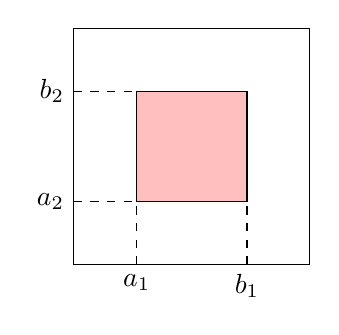
\begin{tikzpicture}
            {
    \def\elemxa{0.8}
    \def\elemxb{2.2}
    \def\elemya{0.8}
    \def\elemyb{2.2}

    \def\minx{0}
    \def\maxx{3}
    \def\miny{0}
    \def\maxy{3}

    \def\firstrect{(\minx,\miny) rectangle (\maxx,\maxy)}
    \def\secondrect{(\elemxa,\elemya) rectangle (\elemxb,\elemyb)}

    \fill[red!25] \secondrect;

    \draw[dashed] (\minx,\elemya) node[left]{$a_2$} -- (\elemxa,\elemya);
    \draw[dashed] (\minx,\elemyb) node[left]{$b_2$} -- (\elemxa,\elemyb);

    \draw[dashed] (\elemxa,\miny) node[below]{$a_1$} -- (\elemxa,\elemya);
    \draw[dashed] (\elemxb,\miny) node[below]{$b_1$} -- (\elemxb,\elemyb);

    \draw[black] \secondrect;
    \draw[black] \firstrect;
}

        \end{tikzpicture}
        \caption{\ref{itm:vert_eigenschaft}. Eigenschaft der Verteilungsfunktion (rote Fläche): ${\mathbb{P}(a_1< X_1\leq b_1,a_2<X_2\leq b_2)}$}
        \label{fig:vert_eigenschaft}
    \end{figure}

    \subsection{Wahrscheinlichkeiten mithilfe der Verteilungsfunktion}\index{Verteilungsfunktion!Wahrscheinlichkeiten|see{Wahrscheinlichkeiten mit Verteilungsfunktion}}\index{Wahrscheinlichkeiten mit Verteilungsfunktion}\label{sec:wahrscheinlichkeiten_verteilungsfunktionen}
    \[\mathbb P(X\le a)=F_X(a),\]
    \[\mathbb P(X<a)=F_X(a-0),\]
    \[\mathbb P(a< X\le b)=F_X(b)-F_X(a),\]
    \[\mathbb P(a< X< b)=F_X(b-0)-F_X(a),\]
    \[\mathbb P(a\le X\le b)=F_X(b)-F_X(a-0),\]
    \[\mathbb P(a\le X< b)=F_X(b-0)-F_X(a-0).\]
    \[\mathbb P( X= a)=F_X(a)-F_X(a-0).\]
    Dabei ist $F(x-0)=\lim\limits_{h\rightarrow 0}F(x-h)$ der linksseitige Grenzwert
    von $F$ in $x$.

    \index{Verteilungsfunktion!{Eigenschaften}|)}


    \section{Unabhängigkeit von Zufallsvariablen}\index{Zufallsvariable!{Unabhängigkeit}|see{Unabhängigkeit von Zufallsvariablen}}\index{Unabhängigkeit von Zufallsvariablen|(}

    \begin{definition}\index{Unabhängigkeit!Verteilung}\label{def:unabhaengigkeit_verteilung}
        Die Zufallsvariablen $(X,Y)$ heißen unabhängig, wenn für
        alle $x_1,\dots x_n$
        \[F_{X_1,\dots,X_n}(x_1,\dots,x_n)=\prod_{i=1}^nF_{X_i}(x_i).\]
        Die unendliche Folge $(X_n,n\in\mathbb N)$ heißt unabhängig, wenn
        jede endliche Teilfolge unabhängig ist.\\


        Wenn die gemeinsame Verteilung diskret bzw. stetig ist, kann man in dieser
        Definition die Verteilungsfunktion durch die Wahrscheinlichkeits- bzw. Dichte-
        funktion ersetzen.
    \end{definition}

    Dafür müssen wir nur die Eigenschaften der Ereignisse auf
    Zufallsvariablen übertragen:

    \begin{definition}
        $X$ und $Y$ heißen unabhängig, wenn $\forall x\in \mathbb R$ und $y\in \mathbb R$
        die Ereignisse $X\le x$ und $Y\le y$ unabhängig sind.

        Das heißt, es muss gelten

        \[
            \mathbb{P}\left(X\le x|Y\le y\right)=\mathbb P(X\le x)
        \]

        oder gleichwertig

        \[
            \mathbb P\left(X\le x\cap Y\le y\right)=
            \mathbb P\left(X\le x\right)\cdot \mathbb P\left(Y\le y\right)
        \]
    \end{definition}

    Mit mehreren Zufallsvariablen muss man wieder zwischen paarweiser und
    totaler Unabhängigkeit unterscheiden. Die $n$ zufälligen Variablen $X_{1},...,X_{n}$
    heißen total unabhängig, wenn für alle $x_{1},...,x_{n}$ gilt:

    \[
    \mathbb P_{X_{1},... ,X_{n}}\left(x_{1},... ,x_{n}\right)=\prod_{i=1}^n{\mathbb P_{i}(x_{i})}
    \]

    \begin{satz}[Faltung von Dichten]\index{Faltung von Dichten}\index{Dichten!Faltung}\label{satz:faltung_dichten} $X$ und $Y$ seien unabhängig mit Dichte $f_X$ und $f_Y$.
        Dann ist die Dichte von $X+Y$ die Faltung von $f_X$ und $f_Y$:
        \[f_{X+Y}(z)=f_X*f_Y(z)=\int_{-\infty}^{\infty} f_X(x)f_Y(z-x)dx.\]
    \end{satz}

    \index{Unabhängigkeit von Zufallsvariablen|)}

    \section{Erwartungswert und Varianz}

    \subsection{Erwartungswert $\mathbb E(X)$ bzw. $\mu_{X}$}\index{Erwartungswert|(}
    \label{sec:erwartungswert}
    Im folgenden Werden die Symbole \gls{symb:mathbbE} und \gls{symb:mu} für den Erwartungswert verwendet.

    \begin{definition}[ von Erwartungswert $\mathbb E$ bzw. $\mu_X$ von $X$]:\\\label{def:erwartungswert}
        Für eine mit Wahrscheinlichkeitsverteilung ${\mathbb P\left(X=x_{j}\right),j=1,2,...,{\infty}}$ verteilte \textbf{diskrete Zufallsvariable} $Y$ gilt:

        \[\mathbb E\left(X\right)=\sum_{j=1}^{{\infty}}{x_{j}\cdot \mathbb P\left(X=x_{j}\right)}\]

        sofern die unendliche Reihe absolut konvergiert. Ansonsten existiert kein Erwartungswert.\\

        Für \textbf{stetige Zufallsvariablen} gilt:
        \[\mathbb E\left(X\right)=\int_{-{\infty}}^{{\infty}}{xf_{X}\left(x\right)}dx\]

        Falls $Y$ \textbf{gemischt verteilt} ist, gilt:
        \[\mathbb E\left(X\right)=\sum_{x}{x\cdot \mathbb P(X=x_{j})}+\int_{-{\infty}}^{{\infty}}{xf_{X}(x)}dx\]
    \end{definition}

    Betrachten wir das anhand unseres Münzspiels (siehe Tabelle \ref{tab:auszahlungen}).\\

    Mit der Wahrscheinlichkeitsverteilung für die Auszahlungen (siehe Abbildung \ref{fig:vert_muenze}):

    \begin{figure}
    \centering
        \begin{tikzpicture}
            {
    \begin{axis}[
        ylabel=Wahrscheinlichkeit,
        xlabel=Auszahlung in Cent,
        axis x line=bottom, % no box around the plot, only x and y axis
        axis y line=left, % the * would suppress the arrow tips
        ymin=0.1,
        ymax=0.6,
        xmin=0.15,
        xmax=100,
        xtick={0,10,30,40,60,80,100},
        enlargelimits=0.15,
        legend pos=north east,
        ybar=-9pt,% configures `bar shift'
        bar width=9pt,
        width=10cm,
        height=5cm,
        clip=false
    ]
    \addplot 
        coordinates {(0,4/8)};

    \addplot 
        coordinates {(20,3/8)};

    \addplot 
        coordinates {(100,1/8)};

    \legend{{0-1x Kopf},{ 2x Kopf },{ 3x Kopf }}

\tikzstyle{vecArrow} = [thick, green, decoration={markings,mark=at position 1 with {\arrow[semithick,green]{open triangle 60}}},
   double distance=1.4pt, shorten >= 5.5pt,
   preaction = {decorate},
   postaction = {draw,line width=1.4pt, white,shorten >= 4.5pt}]

    \node (sp) at (axis cs:20,0.05){};
    \node (down) at (axis cs:20,-0.1){};
    \draw[vecArrow](down)--(sp);

    \end{axis}
}

        \end{tikzpicture}
        \caption{Wahrscheinlichkeitsverteilung für Auszahlung (grüner Pfeil ist Schwerpunkt) siehe Tabelle \ref{tab:auszahlungen}}
        \label{fig:vert_muenze}
    \end{figure}

    Für den Schwerpunkt (grüner Pfeil in Abbildung \ref{fig:vert_muenze}) berechnen wir:

    \[
    \mathbb E\left(X\right)=0\cdot \frac{4}{8}+20\cdot \frac{3}{8}+100\cdot \frac{1}{8}=20
    \]

    \attention {Der Erwartungswert einer Zufallsvariablen ist der Schwerpunkt
    (arithmetisches Mittel) ihrer Verteilung.}

    \subsubsection{Eigenschaften des Erwartungswertes}\index{Erwartungswert!Eigenschaften|see{Eigenschaften des Erwartungswertes}}\index{Eigenschaften des Erwartungswertes}

    \begin{enumerate}[1)]
        \item \textbf{Additivität} Sind $X$, $Y$ zwei Zufallsvariablen, egal ob abhängig oder nicht, mit den
            Erwartungswerten $\mathbb E\left(X\right),\mathbb E\left(Y\right)$, dann gilt:
            \[\mathbb E\left(X+Y\right)=\mathbb E\left(X\right)+\mathbb E(Y)\]
        \item \textbf{Linearität}
            \[\mathbb E\left(aX+b\right)=a\mathbb E\left(X\right)+b\]
        \item \textbf{Monotonie}
            \[X\le Y\Rightarrow \mathbb E\left(X\right)\le \mathbb E(Y)\]
        \item \textbf{Unabhängigkeit}: Wenn $X$ und $Y$ unabhängig sind, dann gilt:
            \[\mathbb E\left(XY\right)=\mathbb E\left(X\right)\mathbb E(Y)\]
    \end{enumerate}

    \begin{satz}\label{satz:unachtsamer_statistiker} \textbf{des unachtsamen Statistikers}\index{Satz des unachtsamen Statistiker}\index{unachtsamer Statistiker!Satz-|see{Satz des unachsamen Statistiker}}
    Siehe Abbildung \ref{fig:unachtsamer_statistiker}.

    $X$ sei stetig verteilt mit der Dichte $f_{X},Y=g\left(X\right)$.
    Um den Erwartungswert von $Y$ zu berechnen, müssen wir nicht die Verteilung von $Y$ berechnen. Wir können
    direkt folgendes Integral verwenden:

    \[\mathbb E\left(Y\right)=\int {g\left(x\right)f_{X}(x)}dx\]

    \end{satz}
    \begin{figure}
    \centering
        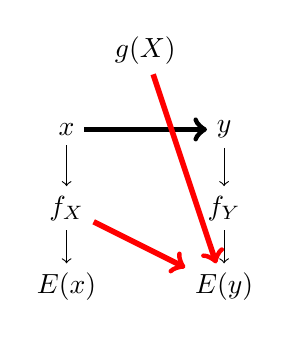
\begin{tikzpicture}
            {
    \def\gxx{0}
    \def\gxy{2}

    \def\xx{-1}
    \def\xy{1}
    \def\yx{1}
    \def\yy{1}

    \def\exx{-1}
    \def\exy{-1}
    \def\eyx{1}
    \def\eyy{-1}

    \def\fxx{-1}
    \def\fxy{0}
    \def\fyx{1}
    \def\fyy{0}

    \node (x) at (\xx,\xy){$x$};
    \node (ex) at (\exx,\exy){$\mathbb E(x)$};
    \node (y) at (\yx,\yy){$y$};
    \node (ey) at (\eyx,\eyy){$\mathbb E(y)$};
    \node (fx) at (\fxx,\fxy){$f_X$};
    \node (fy) at (\fyx,\fyy){$f_Y$};
    \node (gx) at (\gxx,\gxy){$g(X)$};

    \draw[line width=2pt,->](x) -- (y);

    \draw[->](x) -- (fx);
    \draw[->](fx) -- (ex);

    \draw[->](y) -- (fy);
    \draw[->](fy) -- (ey);

    \draw[red,line width=2pt,->](gx) -- (ey);
    \draw[red,line width=2pt,->](fx) -- (ey);
}    
    %\node (sp) at (axis cs:20,0.05){};
    %\node (down) at (axis cs:20,-0.1){};
    %\draw[vecArrow](down)--(sp);

        \end{tikzpicture}
        \caption{Satz des unachtsamen Statistikers (siehe Satz\ref{satz:unachtsamer_statistiker})}
        \label{fig:unachtsamer_statistiker}
    \end{figure}

    \index{Erwartungswert|)}
    \subsection{Varianz}\index{Varianz|(}
    \label{sec:varianz}
    \begin{definition}
    Die Varianz \gls{symb:mathbbV}$(X)$ ist der Mittelwert der quadrierten Abweichungen der
    einzelnen Realisationen vom Schwerpunkt der Verteilung.

    \[\mathbb V\left(X\right)=\mathbb E\left(X-\mathbb E\left(X\right)\right)^{2}=\mathbb E\left(X-\mu\right)^{2}=\sigma ^{2}\]
    \end{definition}

    Für die Berechnung benutzen wir den Erwartungswert (diskret bzw. stetig):

    \[\mathbb V\left(X\right)=\sum_{j=1}^{{\infty}}{\left(x_{j}-\mu\right)^{2}\cdot \mathbb P\left(X=x_{j}\right)}=
    \int_{-{\infty}}^{{\infty}}{\left(x-\mu \right)^{2}f_{X}(x)}dx\]
    \attention{Die Varianz $\mathbb V$ ist ein quadratisches Streuungsmaß}

    \begin{definition}\textbf{Stichprobenvarianz \gls{symb:sn2} mit ML-Schätzer}\index{Stichprobenvarianz!mit ML-Schätzer}
    \index{Varianz!Stichprobe mit ML-Schätzer|see{Stichprobenvarianz!mit ML-Schätzer}}
        \label{def:stichprobenvarianz}%TODO: evtl. noch etwas text
        \[s_n^2= \frac{1}{n} \sum_{i=1}^n\left(x_i-\overline x\right)^2\]
    \end{definition}

    \begin{definition}\textbf{Korrigierte Stichprobenvarianz \gls{symb:sn2}}\index{Stichprobenvarianz!korrigiert|see{Korrigierte Stichprobenvarianz}}\index{Korrigierte Stichprobenvarianz}
        \label{def:korrigierte_stichprobenvarianz}%TODO: evtl. noch etwas text
        \[s_n^2= \frac{1}{n-1} \sum_{i=1}^n\left(x_i-\overline x\right)^2\]
    \end{definition}

    \subsubsection{Verschiebungssatz}
    Wir betrachten die Varianz $\mathbb V\left(X\right)=\mathbb E\left(X-\mathbb E\left(X\right)\right)^{2}$,
    formen um und wenden die Eigenschaften des Erwartungswertes an:

    \[\mathbb V\left(X\right)=\mathbb E\left(X-\mathbb E\left(X\right)\right)^{2}=
        \mathbb E\left(\left(X-\mathbb E\left(X\right)\right)^{2}\right)=
        \mathbb E\left(X^{2}-2X\mathbb E\left(X\right)+\mathbb E\left(X\right)^{2}\right)\]

    Anwendung der Additivität:
    \[\mathbb V\left(X\right)=\mathbb E\left(X^{2}\right)-\mathbb E\left(2X\mathbb E\left(X\right)\right)+\mathbb E\left(\mathbb E\left(X\right)^{2}\right)\]

    Anwendung der Linearität und der Eigenschaft $\mathbb E\left(\mathbb E\left(X\right)\right)=\mathbb E(X)$:
    \[\mathbb V\left(X\right)=\mathbb E\left(X^{2}\right)-2\mathbb E\left(X\mathbb E\left(X\right)\right)+\mathbb E\left(X\right)^{2}=
        \mathbb E\left(X^{2}\right)-2\mathbb E\left(X\right)^{2}+\mathbb E\left(X\right)^{2}\]

    \[\mathbb V\left(X\right)=\mathbb E\left(X^{2}\right)-\mathbb E\left(X\right)^{2}\]

    \begin{satz} Steinerscher Verschiebungssatz\index{Steinerscher Verschiebungssatz}\index{Verschiebungssatz!Steiner-|see{Steinerscher Verschiebungssatz}}
        \label{satz:steinerscher_verschiebungssatz}

    \[
    \mathbb E\left(\left(X-a\right)^{2}\right)=\mathbb V\left(X\right)+\left(\mathbb E\left(X\right)-a\right)^{2}
    \]
    \end{satz}

    \subsubsection{Eigenschaften der Varianz}\index{Varianz!Eigenschaften}
    \begin{definition}[Eigenschaften der Varianz]:\label{def:varianz_eigenschaften}
    \begin{enumerate}[1)]
        \item $\mathbb V\left(X\right)\ge 0$
        \item $\mathbb V\left(X\right)=0$, genau dann, wenn $\mathbb P\left(X=\mathbb E\left(X\right)\right)=1$
        \item $\mathbb V\left(aX+b\right)=a^{2}\mathbb V\left(X\right)$
        \item Wenn $X$ und $Y$ unabhängig sind, dann ist $\mathbb V\left(X+Y\right)=\mathbb V\left(X\right)+\mathbb V(Y)$
    \end{enumerate}
    \end{definition}

    \subsubsection{Kovarianz\index{Kovarianz}}
    \begin{definition}[Kovarianz]:\\
    Die Kovarianz $Cov\left(X,Y\right)$ gibt Aussage darüber, ob hohe Werte
    von $X$ mit hohen Werten von $Y$ oder eher mit niedrigen Werten von $Y$
    einhergehen.

    \begin{itemize}
        \item Die Kovarianz ist positiv, wenn $X$ und $Y$ einen monotonen Zusammenhang
        besitzen, d.h. hohe (niedrige) Werte von $X$ gehen mit hohen (niedrigen)
        Werten von $Y$ einher.
        \item Ist die Kovarianz null, so besteht kein monotoner Zusammenhang zwischen $X$ und $Y$.
    \end{itemize}
    \[Cov\left(X,Y\right)=\mathbb E\left(XY\right)-\mathbb E\left(X\right)\mathbb E\left(Y\right)\]
    \end{definition}
    Damit können wir die Varianz berechnen:
    \[\mathbb V\left(X+Y\right)=\mathbb V\left(X\right)+\mathbb V\left(Y\right)+2Cov\left(X,Y\right)\]
    Wenn die Kovarianz von zwei Zufallsvariablen gleich 0 ist, dann nennen wir sie unkorreliert.

    \subsubsection{Ungleichung von Markov}\index{Ungleichung!von Markov}\index{Markov Ungleichung|see{Ungleichung!von Markov}}
    \begin{definition}[Ungleichung von Markov]:\\
    $X$ sei eine nichtnegative Zufallsvariable und  $\lambda>0$. Dann ist
    \[
    \mathbb P\left(X\ge \lambda \right)\le \frac{1}{\lambda }\mathbb E(X)
    \]
    \end{definition}

    \subsubsection{Ungleichung von Chebychev\index{Ungleichung!von Chebychev}
        \index{Chebychev Ungleichung|see{Ungleichung!von Chebychev}}}

    \begin{definition}[Ungleichung von Chebychev]:\\
        Diese Ungleichung gibt eine allgemeine Schranke an, wie weit eine Zufallsvariable 
        $X$ um ihren Mittelwert streut. Für jede Variable $X$ mit existierender Varianz $\sigma^{2}$ und
        jede beliebige positive Zahl $\lambda$ gilt:

        \[\mathbb P\left(\left|X-\mu \right|\ge \lambda \right)\le \frac{\mathbb V(X)}{\lambda^{2}}\]
        \[\mathbb P\left(\left|X-\mu \right|<\lambda \right)\ge 1-\frac{\mathbb V(X)}{\lambda ^{2}}\]
    \end{definition}

    \begin{bsp}[aus Wikipedia\cite{wiki:002}] Nehmen an, dass Wikipedia-Artikel einen Erwartungswert der Länge von 
    $\mathbb E\left(X\right)=1000$ Zeichen mit einer Standardabweichung von 
    $\sigma_{X}=\sqrt{\mathbb V\left(X\right)}=200$ Zeichen besitzen. 

    Die Wahrscheinlichkeit, dass ein Wikipedia-Artikel eine
    Länge zwischen $600$ und $1400$ $\left(\Rightarrow \lambda=400\right)$ Zeichen hat, berechne sich mit:

    \[
        \mathbb P\left|\left(X-1000\right|<400\right)=1-\frac{200^{2}}{400^{2}}=1-\frac{1}{4}=75
    \]
    \end{bsp}

    \subsubsection{Ungleichung von Kolmogorov\index{Ungleichung!von Kolmogorov}
        \index{Kolmogorov Ungleichung|see{Ungleichung!von Kolmogorov}}}
    \begin{definition}\textbf{Kolmogorov-Ungleichung}
    Die Kolmogorov-Ungleichung ist eine sogenannte Maximal-Ungleichung aus
    der Stochastik. Seien $X_{1},... ,X_{n}$ unabhängige Zufallsvariablen mit
    Erwartungswert 0, und zusätzlich $S_{0}=0,$ und $S_{n}=X_{1}+... +X_{n}$. Dann ist

    \[\mathbb P\left(\max_{k\le n}\left(S_{k}\right)\ge \lambda\right)\le 
        \frac{\mathbb V\left(S_{n}\right)}{\lambda ^{2}}\]
    \end{definition}
    
    \index{Varianz|)}


    \section{Folgen von Zufallsvariablen}\index{Zufallsvariable!Folgen|see{Folgen von Zufallsvariablen}}\index{Folgen von Zufallsvariablen|(}

    Nun untersuchen wir Folgen von Zufallsvariablen $X_{1},...,X_{n},$ die unabhängig und identisch
    verteilt sind, abgekürzt \gls{symb:iid} (independent and identically distributed). 
    Einfachstes Beispiel sind drei unabhängige Münzwürfe.

    \subsection{Schwaches Gesetz der großen Zahlen\index{Gesetz!Schwaches G. der gr. Z.|see{Schwaches G. der gr. Z.}}\index{Schwaches G. der gr. Z.|(}}

    Bei geringem Stichprobenumfang n ist die Chebychev-Ungleichung sehr
    ungenau, sie wird aber genauer, je größer n wird. Wir gehen von n
    Zufallsvariablen aus und bilden uns den Mittelwert:

    \[\overline{X}^{\left(n\right)}=\frac{1}{n}\sum_{i=1}^{n}X_{i}\]

    Der Erwartungswert von i.i.d Zufallsvariablen ist immer gleich, somit gilt:

    \[\mathbb E\left(\overline{X}^{\left(n\right)}\right)=\mu\]

    Da die Varianz ein quadratisches Streuungsmaß ist, folgt:

    \[\mathbb V\left(\overline{X}^{\left(n\right)}\right)=
        \mathbb V\left(\frac{1}{n}\sum_{i=1}^{n}X_{i}\right)=
        \frac{1}{n^{2}}\mathbb V\left(\sum_{i=1}^{n}X_{i}\right)\]

    denn beim Ausklammern der Konstante $\frac{1}{n}$ wird diese quadriert.

    \[\frac{1}{n^{2}}\mathbb V\left(\sum_{i=1}^{n}X_{i}\right)=\frac{1}{n^{2}}n\sigma ^{2}=\frac{\sigma^{2}}{n}\]

    \attention {Die letzte Umformung kommt aus der Summenregel für unkorrelierte
    Zufallsvariablen: $\mathbb V\left(\sum _{i=1}^{n}X_{i}\right)=\sum _{i=1}^{n}{\mathbb V(X_{i})}$}

    Nun benutzen wir die Ungleichung von Chebychev und passen sie an:

    \[\mathbb P\left(\left|{\overline{X}}^{\left(n\right)}-\mu
    \right|<\lambda \right)\ge 1-\frac{\frac{\sigma ^{2}}{n}}{\lambda
    ^{2}}\]
    \[\mathbb P\left(\left|{\overline{X}}^{\left(n\right)}-\mu \right|<\lambda
    \right)\ge 1-\frac{\sigma ^{2}}{n\lambda ^{2}}\]

    Schlussendlich schicken wir n gegen unendlich und beachten, dass die
    Wahrscheinlichkeit nie größer als Eins werden kann:

    \[\lim_{n\rightarrow{\infty}}\mathbb P\left(\left|{\overline{X}}^{\left(n\right)}-\mu
    \right|<\lambda \right)\ge 1\]
    \begin{definition}\textbf{Schwaches Gesetz der großen Zahlen}\\
        Es sei $\left(X_{n}\right)_{n\in N}$ eine Folge von i.i.d.-zufälligen Variablen mit 
        $\mathbb E\left(X_{n}\right)=\mu$. Dann gilt $\forall\epsilon >0$:

    \[\lim_{n\rightarrow\infty}\mathbb P\left(\left|{\overline{X}}^{\left(n\right)}-\mu
    \right|<\epsilon \right)=1\]
    \end{definition}

    Das schwache Gesetz der großen Zahlen sagt uns also, dass mit
    steigender Anzahl von Zufallsvariablen große Abweichungen immer
    unwahrscheinlicher werden.

    \index{Schwaches G. der gr. Z.|)}

    \subsection{Starkes Gesetz der großen Zahlen\index{Gesetz!Starkes G. der gr. Z.|see{Starkes G. der gr. Z.}}\index{Starkes G. der gr. Z.|(}}\label{sec:starkes_gesetz_grossen_zahlen}

    Das starke Gesetz der großen Zahlen bedeutet, dass
    \[\lim_{n\rightarrow\infty}{\overline{X}}^{\left(n\right)}=\mu\]
    nicht immer, aber {\quotedblbase}so gut wie immer{\textquotedblleft}
    gilt.

    \begin{definition}
    Es sei $\left(X_{n}\right)_{n\in \mathbb N}$ eine
    Folge von i.i.d.-zufälligen Variablen mit
    ${\mathbb E\left(X_{i}\right)=\mu}$
    Dann gilt:

    \[\mathbb P\left(\underset{n\rightarrow
    {\infty}}{{lim}}{\overline{X}}^{\left(n\right)}=\mu \right)=1\]

    Man sagt: ${\overline{X}}^{\left(n\right)}$ konvergiert fast sicher gegen $\mu$.
    \end{definition}
    \index{Starkes G. der gr. Z.|)}

    \subsection{Zentraler Grenzwertsatz\index{Grenzwertsatz!Zentraler-|see{Zentraler Grenzwertsatz}}\index{Zentraler Grenzwertsatz|(}}

    Dafür führen wir zuerst den Begriff der standardisieren Zufallsvariable ein.

    \begin{definition}\textbf{Standardisierte Zufallsvariable}\index{Standardisierte Zufallsvariable}\index{Zufallsvariable!standardisierte}\\
    Eine Zufallsvariable $X$ mit Erwartungswert gleich null und Varianz gleich
    eins heißt standardisierte Zufallsvariable. Ist $X$ eine beliebige
    Zufallsvariable mit $\mathbb E\left(X\right)=\mu$ und $\mathbb V\left(X\right)=\sigma^{2}$,
    dann heißt 
    \[X^*=\frac{X-\mu }{\sigma }\]
    $\sigma$ bezeichnet dabei die Standardabweichung $\sigma=\sqrt{\mathbb V\left(X\right)}$

    die Standardisierte von $X$. Der Vorgang selbst heißt Standardisierung. Für die standardisierte Variable $X^*$ gilt:

    \[\mathbb E\left(X^*\right)=0\]
    \[\mathbb V\left(X^*\right)=1\]
    \end{definition}

    Beim zentralen Grenzwertsatz berechnen wir zuerst die Summe von $n$ i.i.d. Zufallsvariablen mit 
    $\mathbb E\left(X\right)=\mu $ und $\mathbb V\left(X\right)=\sigma^{2}$:

    \[S_{n}=X_{1}+\ldots +X_{n}\]
    \[\mathbb E\left(S_{n}\right)=n\mu\]
    \[\mathbb V\left(S_{n}\right)=n\sigma^{2}\]

    Wir standardisieren $S_{n}$:
    \[S_{n}^*=\frac{S_{n}-n\mu}{\sqrt{n\sigma^{2}}}\]

    \begin{satz}\textbf{Zentraler Grenzwertsatz:}\label{satz:zentraler_grenzwertsatz}\\
    Der zentrale Grenzwertsatz besagt, dass die Verteilungsfunktion 
    $S_{n}^*$ für $n\rightarrow\infty$
    punktweise gegen die Verteilungsfunktion der Standardnormalverteilung $\mathcal N\left(0,1\right)$ konvergiert. 
    Ist $\Phi\left(z\right)$ die Verteilungsfunktion von $\mathcal N\left(0,1\right)$, 
    dann bedeutet dies, dass für jedes reelle $z$ gilt:

    \[\lim_{n\rightarrow\infty}\mathbb P\left(S_{n}^*\le z\right)=
    \lim_{n\rightarrow\infty}\mathbb P\left(\frac{S_{n}-n\mu}{\sqrt{n\sigma^{2}}}\le z\right)=
    \Phi \left(z\right)=\int_{-\infty}^{z}{\frac{1}{\sqrt{2\pi}}e^{\frac{-x^{2}}{2}}}dx\]
    \end{satz}

    \index{Zentraler Grenzwertsatz|)}
    \index{Folgen von Zufallsvariablen|)}

    \section{Diskrete Verteilungen}\index{Verteilung!Diskret|see{Diskrete Verteilung}}\index{Diskrete Verteilung|(}\label{sec:diskrete_verteilungen}

    \subsection{Binomialverteilung\index{Binomialverteilung}\index{Verteilung!Binomial-|see{Binomialverteilung}}}\label{sec:binomialverteilung}
    \label{sec:binomialverteilung}
    {
        \begin{figure}
            \def\nval{30}
            \subfigure[Wahrscheinlichkeitsfunktion mit $n=\nval$]{
                \begin{tikzpicture}
                    {
    \def\pvala{0.5}
    \def\pvalb{0.25}
    \def\pvalc{0.75}
    \def\pvald{0.9}

    \pgfmathtruncatemacro{\maxval}{\nval}

    \begin{axis}[
        domain=-4:4,
        axis x line=bottom, % no box around the plot, only x and y axis
        axis y line=left, % the * would suppress the arrow tips
        legend style={at={(0.67\nval,1.2)}},
        xlabel={k},
        ylabel={p},%TODO: was ist diese Achse?
        samples=200,
        height=5cm,
        width=7cm,
        clip=false]

        \pgfkeys{/pgf/fpu=true}
        \pgfkeys{/pgf/number format/.cd,fixed,precision=5}

        \def\x{1}
        \pgfmathparse{binomial_distribution(\nval,\x,\pvalb)}
        \addplot[continuityblue] coordinates{(\x,\pgfmathresult)};
        \addlegendentry[align=left]{\scriptsize{$\mathcal B(k|\nval,\pvalb)$}};

        \pgfmathparse{binomial_distribution(\nval,\x,\pvalc)}
        \addplot[continuitygreen] coordinates{(\x,\pgfmathresult)};
        \addlegendentry[align=left]{\scriptsize{$\mathcal B(k|\nval,\pvalc)$}};

        \pgfmathparse{binomial_distribution(\nval,\x,\pvald)}
        \addplot[continuityorange] coordinates{(\x,\pgfmathresult)};
        \addlegendentry[align=left]{\scriptsize{$\mathcal B(k|\nval,\pvald)$}};

        \pgfmathparse{binomial_distribution(\nval,\x,\pvala)}
        \addplot[continuityred] coordinates{(\x,\pgfmathresult)};
        \addlegendentry[align=left]{\scriptsize{$\mathcal B(k|\nval,\pvala)$}};

        \foreach \x in {2,...,\maxval} {
            \pgfkeys{/pgf/fpu=false}
            \pgfmathtruncatemacro{\nextx}{\x+1}
            \pgfkeys{/pgf/fpu=true}
            \pgfkeys{/pgf/number format/.cd,fixed,precision=5}

            \pgfmathparse{binomial_distribution(\nval,\x,\pvalb)}
            \addplot[continuityblue,forget plot] coordinates{(\x,\pgfmathresult)};

            \pgfmathparse{binomial_distribution(\nval,\x,\pvalc)}
            \addplot[continuitygreen,forget plot] coordinates{(\x,\pgfmathresult)};

            \pgfmathparse{binomial_distribution(\nval,\x,\pvald)}
            \addplot[continuityorange,forget plot] coordinates{(\x,\pgfmathresult)};

            \pgfmathparse{binomial_distribution(\nval,\x,\pvala)}
            \addplot[continuityred,forget plot] coordinates{(\x,\pgfmathresult)};
        }
        \pgfkeys{/pgf/fpu=false}


    \end{axis}
}
            
                \end{tikzpicture}
                \label{fig:binomial_dist_a}
            }
            \def\nval{15}
            \subfigure[Wahrscheinlichkeitsfunktion mit $n=\nval$]{
                \begin{tikzpicture}
                    {
    \def\pvala{0.5}
    \def\pvalb{0.25}
    \def\pvalc{0.75}
    \def\pvald{0.9}

    \pgfmathtruncatemacro{\maxval}{\nval}

    \begin{axis}[
        domain=-4:4,
        axis x line=bottom, % no box around the plot, only x and y axis
        axis y line=left, % the * would suppress the arrow tips
        legend style={at={(0.67\nval,1.2)}},
        xlabel={k},
        ylabel={p},%TODO: was ist diese Achse?
        samples=200,
        height=5cm,
        width=7cm,
        clip=false]

        \pgfkeys{/pgf/fpu=true}
        \pgfkeys{/pgf/number format/.cd,fixed,precision=5}

        \def\x{1}
        \pgfmathparse{binomial_distribution(\nval,\x,\pvalb)}
        \addplot[continuityblue] coordinates{(\x,\pgfmathresult)};
        \addlegendentry[align=left]{\scriptsize{$\mathcal B(k|\nval,\pvalb)$}};

        \pgfmathparse{binomial_distribution(\nval,\x,\pvalc)}
        \addplot[continuitygreen] coordinates{(\x,\pgfmathresult)};
        \addlegendentry[align=left]{\scriptsize{$\mathcal B(k|\nval,\pvalc)$}};

        \pgfmathparse{binomial_distribution(\nval,\x,\pvald)}
        \addplot[continuityorange] coordinates{(\x,\pgfmathresult)};
        \addlegendentry[align=left]{\scriptsize{$\mathcal B(k|\nval,\pvald)$}};

        \pgfmathparse{binomial_distribution(\nval,\x,\pvala)}
        \addplot[continuityred] coordinates{(\x,\pgfmathresult)};
        \addlegendentry[align=left]{\scriptsize{$\mathcal B(k|\nval,\pvala)$}};

        \foreach \x in {2,...,\maxval} {
            \pgfkeys{/pgf/fpu=false}
            \pgfmathtruncatemacro{\nextx}{\x+1}
            \pgfkeys{/pgf/fpu=true}
            \pgfkeys{/pgf/number format/.cd,fixed,precision=5}

            \pgfmathparse{binomial_distribution(\nval,\x,\pvalb)}
            \addplot[continuityblue,forget plot] coordinates{(\x,\pgfmathresult)};

            \pgfmathparse{binomial_distribution(\nval,\x,\pvalc)}
            \addplot[continuitygreen,forget plot] coordinates{(\x,\pgfmathresult)};

            \pgfmathparse{binomial_distribution(\nval,\x,\pvald)}
            \addplot[continuityorange,forget plot] coordinates{(\x,\pgfmathresult)};

            \pgfmathparse{binomial_distribution(\nval,\x,\pvala)}
            \addplot[continuityred,forget plot] coordinates{(\x,\pgfmathresult)};
        }
        \pgfkeys{/pgf/fpu=false}


    \end{axis}
}
            
                \end{tikzpicture}
                \label{fig:binomial_dist_b}
            }

            \def\nval{30}
            \subfigure[Binomialverteilung mit $n=\nval$]{
                \begin{tikzpicture}
                    {
    \def\pvala{0.5}
    \def\pvalb{0.25}
    \def\pvalc{0.75}
    \def\pvald{0.9}

    \pgfmathtruncatemacro{\maxval}{\nval}

    \begin{axis}[
        domain=-4:4,
        axis x line=bottom, % no box around the plot, only x and y axis
        axis y line=left, % the * would suppress the arrow tips
        legend pos=north west,
        xlabel={k},
        ylabel={p},%TODO: was ist diese Achse?
        samples=200,
        height=5cm,
        width=7cm,
        clip=false]

        \pgfkeys{/pgf/fpu=true}
        \pgfkeys{/pgf/number format/.cd,fixed,precision=5}

        \def\x{1}
        \def\nextx{2}
        %\foreach \x/\y [remember=\x as \lastx (initially A)] in {B/2,C/3,D/4,E/5}
        \pgfmathparse{binomial_distribution(\nval,\x,\pvalb)}
        \xdef\tvalb{\pgfmathresult}
        \addplot[blue,forget plot] coordinates{(\x,\tvalb)(\nextx,\tvalb)};
        \addplot[continuityblue] coordinates{(\x,\tvalb)};
        \addlegendentry[align=left]{\scriptsize{$\mathcal B(k|\nval,\pvalb)$}};

        \pgfmathparse{binomial_distribution(\nval,\x,\pvalc)}
        \xdef\tvalc{\pgfmathresult}
        \addplot[green,forget plot] coordinates{(\x,\tvalc)(\nextx,\tvalc)};
        \addplot[continuitygreen] coordinates{(\x,\tvalc)};
        \addlegendentry[align=left]{\scriptsize{$\mathcal B(k|\nval,\pvalc)$}};

        \pgfmathparse{binomial_distribution(\nval,\x,\pvald)}
        \xdef\tvald{\pgfmathresult}
        \addplot[orange,forget plot] coordinates{(\x,\tvald)(\nextx,\tvald)};
        \addplot[continuityorange] coordinates{(\x,\tvald)};
        \addlegendentry[align=left]{\scriptsize{$\mathcal B(k|\nval,\pvald)$}};

        \pgfmathparse{binomial_distribution(\nval,\x,\pvala)}
        \xdef\tvala{\pgfmathresult}
        \addplot[red,forget plot] coordinates{(\x,\tvala)(\nextx,\tvala)};
        \addplot[continuityred] coordinates{(\x,\tvala)};
        \addlegendentry[align=left]{\scriptsize{$\mathcal B(k|\nval,\pvala)$}};

        \foreach \x [remember=\x as \lastx (initially 0)] in {2,...,\maxval} {
            \pgfkeys{/pgf/fpu=false}
            \pgfmathtruncatemacro{\nextx}{\x+1}
            \pgfkeys{/pgf/fpu=true}
            \pgfkeys{/pgf/number format/.cd,fixed,precision=5}

            \pgfmathparse{\tvalb+binomial_distribution(\nval,\x,\pvalb)}
            \xdef\tvalb{\pgfmathresult}
            \addplot[blue,forget plot] coordinates{(\x,\tvalb)(\nextx,\tvalb)};
            \addplot[continuityblue,forget plot] coordinates{(\x,\tvalb)};

            \pgfmathparse{\tvalc+binomial_distribution(\nval,\x,\pvalc)}
            \xdef\tvalc{\pgfmathresult}
            \addplot[green,forget plot] coordinates{(\x,\tvalc)(\nextx,\tvalc)};
            \addplot[continuitygreen,forget plot] coordinates{(\x,\tvalc)};

            \pgfmathparse{\tvald+binomial_distribution(\nval,\x,\pvald)}
            \xdef\tvald{\pgfmathresult}
            \addplot[orange,forget plot] coordinates{(\x,\tvald)(\nextx,\tvald)};
            \addplot[continuityorange,forget plot] coordinates{(\x,\tvald)};

            \pgfmathparse{\tvala+binomial_distribution(\nval,\x,\pvala)}
            \xdef\tvala{\pgfmathresult}
            \addplot[red,forget plot] coordinates{(\x,\tvala)(\nextx,\tvala)};
            \addplot[continuityred,forget plot] coordinates{(\x,\tvala)};
        }
        \pgfkeys{/pgf/fpu=false}


    \end{axis}
}
            
                \end{tikzpicture}
                \label{fig:binomial_dist_c}
            }
            \def\nval{15}
            \subfigure[Binomialverteilung mit $n=\nval$]{
                \begin{tikzpicture}
                    {
    \def\pvala{0.5}
    \def\pvalb{0.25}
    \def\pvalc{0.75}
    \def\pvald{0.9}

    \pgfmathtruncatemacro{\maxval}{\nval}

    \begin{axis}[
        domain=-4:4,
        axis x line=bottom, % no box around the plot, only x and y axis
        axis y line=left, % the * would suppress the arrow tips
        legend pos=north west,
        xlabel={k},
        ylabel={p},%TODO: was ist diese Achse?
        samples=200,
        height=5cm,
        width=7cm,
        clip=false]

        \pgfkeys{/pgf/fpu=true}
        \pgfkeys{/pgf/number format/.cd,fixed,precision=5}

        \def\x{1}
        \def\nextx{2}
        %\foreach \x/\y [remember=\x as \lastx (initially A)] in {B/2,C/3,D/4,E/5}
        \pgfmathparse{binomial_distribution(\nval,\x,\pvalb)}
        \xdef\tvalb{\pgfmathresult}
        \addplot[blue,forget plot] coordinates{(\x,\tvalb)(\nextx,\tvalb)};
        \addplot[continuityblue] coordinates{(\x,\tvalb)};
        \addlegendentry[align=left]{\scriptsize{$\mathcal B(k|\nval,\pvalb)$}};

        \pgfmathparse{binomial_distribution(\nval,\x,\pvalc)}
        \xdef\tvalc{\pgfmathresult}
        \addplot[green,forget plot] coordinates{(\x,\tvalc)(\nextx,\tvalc)};
        \addplot[continuitygreen] coordinates{(\x,\tvalc)};
        \addlegendentry[align=left]{\scriptsize{$\mathcal B(k|\nval,\pvalc)$}};

        \pgfmathparse{binomial_distribution(\nval,\x,\pvald)}
        \xdef\tvald{\pgfmathresult}
        \addplot[orange,forget plot] coordinates{(\x,\tvald)(\nextx,\tvald)};
        \addplot[continuityorange] coordinates{(\x,\tvald)};
        \addlegendentry[align=left]{\scriptsize{$\mathcal B(k|\nval,\pvald)$}};

        \pgfmathparse{binomial_distribution(\nval,\x,\pvala)}
        \xdef\tvala{\pgfmathresult}
        \addplot[red,forget plot] coordinates{(\x,\tvala)(\nextx,\tvala)};
        \addplot[continuityred] coordinates{(\x,\tvala)};
        \addlegendentry[align=left]{\scriptsize{$\mathcal B(k|\nval,\pvala)$}};

        \foreach \x [remember=\x as \lastx (initially 0)] in {2,...,\maxval} {
            \pgfkeys{/pgf/fpu=false}
            \pgfmathtruncatemacro{\nextx}{\x+1}
            \pgfkeys{/pgf/fpu=true}
            \pgfkeys{/pgf/number format/.cd,fixed,precision=5}

            \pgfmathparse{\tvalb+binomial_distribution(\nval,\x,\pvalb)}
            \xdef\tvalb{\pgfmathresult}
            \addplot[blue,forget plot] coordinates{(\x,\tvalb)(\nextx,\tvalb)};
            \addplot[continuityblue,forget plot] coordinates{(\x,\tvalb)};

            \pgfmathparse{\tvalc+binomial_distribution(\nval,\x,\pvalc)}
            \xdef\tvalc{\pgfmathresult}
            \addplot[green,forget plot] coordinates{(\x,\tvalc)(\nextx,\tvalc)};
            \addplot[continuitygreen,forget plot] coordinates{(\x,\tvalc)};

            \pgfmathparse{\tvald+binomial_distribution(\nval,\x,\pvald)}
            \xdef\tvald{\pgfmathresult}
            \addplot[orange,forget plot] coordinates{(\x,\tvald)(\nextx,\tvald)};
            \addplot[continuityorange,forget plot] coordinates{(\x,\tvald)};

            \pgfmathparse{\tvala+binomial_distribution(\nval,\x,\pvala)}
            \xdef\tvala{\pgfmathresult}
            \addplot[red,forget plot] coordinates{(\x,\tvala)(\nextx,\tvala)};
            \addplot[continuityred,forget plot] coordinates{(\x,\tvala)};
        }
        \pgfkeys{/pgf/fpu=false}


    \end{axis}
}
            
                \end{tikzpicture}
                \label{fig:binomial_dist_d}
            }
            \caption{Die Binomialverteilung}
            \label{fig:binomial_dist}
        \end{figure}
    }

    \begin{bsp}\textbf{Münzwurf:}\\ 
    Bezeichnen wir die Wahrscheinlichkeit von \textbf{Kopf mit} $p$, so ergibt sich die Wahrscheinlichkeit von 
    \textbf{Zahl} mit $1-p$.

    Ist $X$ die Anzahl der Kopfwürfe bei $n$ Würfen, so tritt das Ereignis $X=k$ genau dann auf, wenn in einer
    Wurfsequenz $(... K ... Z ... Z ...)$ genau $k$-mal $K$ auftritt und daher auch $(n-k)$ mal $Z$. 
    Die Wahrscheinlichkeit einer solchen Sequenz ist 
    \[p^{k}\left(1-p\right)^{n-k}\]
    Dabei kann die Reihenfolge egal sein. Wir müssen also noch wissen, wie viele Möglichkeiten es gibt, 
    aus $n$ Würfen, $k$ auszuwählen:

    \[\binom{n}{k}\]
    \end{bsp}

    Sie beschreibt die Anzahl der Erfolge in einer Serie von gleichartigen und unabhängigen Versuchen, die jeweils genau zwei mögliche Ergebnisse haben („Erfolg“ oder „Misserfolg“). (Wikipedia \cite{wiki:003})

    Damit haben wir die Binomialverteilung (siehe Abbildung \ref{fig:binomial_dist}) definiert:
    \begin{definition}\textbf{Binomialverteilung}
    \[
    \mathcal B\left(k|n,p\right)=
    \binom{n}{k}p^{k}\left(1-p\right)^{n-k}k=0,1,...,n
    \]
    \[\mathbb E\left(X\right)=np\]
    \[\mathbb V\left(X\right)=np(1-p)\]
    \end{definition}

    Für die Binomialverteilung existiert ein \textbf{Additionstheorem}:

    \[\text{Aus}
        \begin{cases}X\sim\mathcal B_n(\theta)\\Y\sim\mathcal B_n(\theta)\end{cases} 
        \text{folgt}X+Y\sim\mathcal B_{n+m}(\theta)\]

    Existieren nicht nur zwei Möglichkeiten, kann die Binomialverteilung mit der Polynomialverteilung
    vertauscht werden. Es sind $r,w,... ,g$ die Anzahl der einzelnen Elemente (z.B. rote, weiße und grüne) und 
    $\theta_{r},\theta_{w},...,\theta_{g}$ die entsprechenden Wahrscheinlichkeiten:

    \[
    \mathbb P\left(r,w,\ldots ,g\right)=
        \frac{n!}{r!w!\ldots g!}\left(\theta_{r}\right)^{r}\left(\theta_{w}\right)^{w}\ldots \left(\theta_{g}\right)^{g}
    \]

    \subsection{Gleichverteilung\index{Gleichverteilung!diskret}\index{Verteilung!Gleich-(diskret)|see{Gleichverteilung!diskret}}}\label{sec:gleichverteilung_diskret}

    {
        \begin{figure}
            \def\bval{10}
            \def\aval{2}
            \subfigure[Wahrscheinlichkeitsfunktion]{
                \begin{tikzpicture}
                    {
    \begin{axis}[
        domain=-4:4,
        axis x line=bottom, % no box around the plot, only x and y axis
        axis y line=left, % the * would suppress the arrow tips
        legend pos=north west,
        xlabel={k},
        ylabel={p},%TODO: was ist diese Achse?
        samples=200,
        height=5cm,
        width=7cm,
        clip=false]

        \pgfkeys{/pgf/fpu=true}
        \pgfkeys{/pgf/number format/.cd,fixed,precision=5}

        \def\x{1}
        \addplot[continuityblue] coordinates{(\x,0)};
        \addlegendentry[align=left]{\scriptsize{$\mathcal D(\aval,\bval)$}};

        \foreach \x in {\aval,...,\bval} {
            \pgfkeys{/pgf/fpu=false}
            \pgfmathtruncatemacro{\nextx}{\x+1}
            \pgfkeys{/pgf/fpu=true}
            \pgfkeys{/pgf/number format/.cd,fixed,precision=5}

            \pgfmathparse{1/(\bval-\aval+1)}
            \addplot[continuityblue,forget plot] coordinates{(\x,\pgfmathresult)};
        }

        \pgfkeys{/pgf/fpu=false}

        \pgfmathtruncatemacro{\x}{\bval+1}
        \addplot[continuityblue] coordinates{(\x,0)};
    \end{axis}
}
            
                \end{tikzpicture}
                \label{fig:gleich_dist_a}
            }
            \subfigure[Gleichverteilung]{
                \begin{tikzpicture}
                    {
    \begin{axis}[
        domain=-4:4,
        axis x line=bottom, % no box around the plot, only x and y axis
        axis y line=left, % the * would suppress the arrow tips
        legend pos=north west,
        xlabel={k},
        ylabel={p},%TODO: was ist diese Achse?
        samples=200,
        height=5cm,
        width=7cm,
        clip=false]

        \pgfkeys{/pgf/fpu=true}
        \pgfkeys{/pgf/number format/.cd,fixed,precision=5}

        \def\x{1}
        \def\nextx{2}
        \addplot[continuityblue] coordinates{(\x,0)};
        \xdef\tval{0}
        \addplot[blue,forget plot] coordinates{(\x,\tval)(\nextx,\tval)};
        \addplot[continuityblue] coordinates{(\x,\tval)};
        \addlegendentry[align=left]{\scriptsize{$\mathcal D(\aval,\bval)$}};

        \foreach \x [remember=\x as \lastx (initially 0)] in {\aval,...,\bval} {
            \pgfkeys{/pgf/fpu=false}
            \pgfmathtruncatemacro{\nextx}{\x+1}
            \pgfkeys{/pgf/fpu=true}
            \pgfkeys{/pgf/number format/.cd,fixed,precision=5}

            \pgfmathparse{\tval+1/(\bval-\aval+1)}
            \xdef\tval{\pgfmathresult}
            \addplot[blue,forget plot] coordinates{(\x,\tval)(\nextx,\tval)};
            \addplot[continuityblue,forget plot] coordinates{(\x,\tval)};

        }
        \pgfkeys{/pgf/fpu=false}


    \end{axis}
}
            
                \end{tikzpicture}
                \label{fig:gleich_dist_b}
            }
            \caption{Die Gleichverteilung}
            \label{fig:gleich_dist}
        \end{figure}
    }

    \begin{bsp}
    Die Gleichverteilung beschreibt den Wurf eines idealen $n$-Seiten Würfels. (siehe Abbildung \ref{fig:gleich_dist})
    \end{bsp}

    \begin{definition}
    \[\mathbb P\left(X=k\right)=\frac{1}{n}\]
    \[\mathbb E\left(X\right)=\frac{n+1}{2}\]
    \[\mathbb V\left(X\right)=\frac{n^{2}-1}{12}\]
    \end{definition}
    
    Befindet sich $k$ in einem beliebigen Intervall $a\leq k\le b$, so gilt analog:

    \[\mathbb P\left(X=k\right)=\frac{1}{b-a+1}\]
    \[\mathbb E\left(X\right)=\frac{b+a}{2}\]
    \[\mathbb V\left(X\right)=\frac{\left(b-a\right)^{2}-1}{12}\]
    
    \subsection{Geometrische Verteilung\index{Geometrische Verteilung}\index{Verteilung!Geometrische-|see{Geometrische Verteilung}}}
    \label{sec:geometrische_verteilung}
    {
        \begin{figure}
            \def\nval{10}
            \def\pvala{0.8}
            \def\pvalb{0.5}
            \def\pvalc{0.2}
            \subfigure[Wahrscheinlichkeitsfunktion]{
                \begin{tikzpicture}
                    {
    \begin{axis}[
        domain=-4:4,
        axis x line=bottom, % no box around the plot, only x and y axis
        axis y line=left, % the * would suppress the arrow tips
        legend pos=north east,
        ymin=0,
        ymax=1,
        xlabel={k},
        ylabel={p},%TODO: was ist diese Achse?
        samples=200,
        height=5cm,
        width=7cm,
        clip=false]

        \pgfkeys{/pgf/fpu=true}
        \pgfkeys{/pgf/number format/.cd,fixed,precision=5}

        \def\x{1}
        \pgfmathparse{\pvala*(1-\pvala)^(\x-1)}
        \addplot[continuityblue] coordinates{(\x,\pgfmathresult)};
        \addlegendentry[align=left]{\scriptsize{$\mathcal G(\pvala)$}};

        \pgfmathparse{\pvalb*(1-\pvalb)^(\x-1)}
        \addplot[continuityred] coordinates{(\x,\pgfmathresult)};
        \addlegendentry[align=left]{\scriptsize{$\mathcal G(\pvalb)$}};

        \pgfmathparse{\pvalc*(1-\pvalc)^(\x-1)}
        \addplot[continuitygreen] coordinates{(\x,\pgfmathresult)};
        \addlegendentry[align=left]{\scriptsize{$\mathcal G(\pvalc)$}};

        \foreach \x in {2,...,\nval} {
            \pgfkeys{/pgf/fpu=false}
            \pgfmathtruncatemacro{\nextx}{\x+1}
            \pgfkeys{/pgf/fpu=true}
            \pgfkeys{/pgf/number format/.cd,fixed,precision=5}

            \pgfmathparse{\pvala*(1-\pvala)^(\x-1)}
            \addplot[continuityblue,forget plot] coordinates{(\x,\pgfmathresult)};

            \pgfmathparse{\pvalb*(1-\pvalb)^(\x-1)}
            \addplot[continuityred,forget plot] coordinates{(\x,\pgfmathresult)};

            \pgfmathparse{\pvalc*(1-\pvalc)^(\x-1)}
            \addplot[continuitygreen,forget plot] coordinates{(\x,\pgfmathresult)};
        }

        \pgfkeys{/pgf/fpu=false}
    \end{axis}
}
            
                \end{tikzpicture}
                \label{fig:geomet_dist_a}
            }
            \subfigure[Geometrische Verteilung]{
                \begin{tikzpicture}
                    {
    \begin{axis}[
        domain=-4:4,
        axis x line=bottom, % no box around the plot, only x and y axis
        axis y line=left, % the * would suppress the arrow tips
        legend pos=south east,
        ymin=0,
        ymax=1,
        xlabel={k},
        ylabel={p},%TODO: was ist diese Achse?
        samples=200,
        height=5cm,
        width=7cm,
        clip=false]

        \pgfkeys{/pgf/fpu=true}
        \pgfkeys{/pgf/number format/.cd,fixed,precision=5}

        \def\x{1}
        \def\nextx{2}
        \pgfmathparse{\pvala*(1-\pvala)^(\x-1)}
        \xdef\tvala{\pgfmathresult}
        \addplot[blue,forget plot] coordinates{(\x,\tvala)(\nextx,\tvala)};
        \addplot[continuityblue] coordinates{(\x,\pgfmathresult)};
        \addlegendentry[align=left]{\scriptsize{$\mathcal G(\pvala)$}};

        \pgfmathparse{\pvalb*(1-\pvalb)^(\x-1)}
        \xdef\tvalb{\pgfmathresult}
        \addplot[red,forget plot] coordinates{(\x,\tvalb)(\nextx,\tvalb)};
        \addplot[continuityred] coordinates{(\x,\pgfmathresult)};
        \addlegendentry[align=left]{\scriptsize{$\mathcal G(\pvalb)$}};

        \pgfmathparse{\pvalc*(1-\pvalc)^(\x-1)}
        \xdef\tvalc{\pgfmathresult}
        \addplot[green,forget plot] coordinates{(\x,\tvalc)(\nextx,\tvalc)};
        \addplot[continuitygreen] coordinates{(\x,\pgfmathresult)};
        \addlegendentry[align=left]{\scriptsize{$\mathcal G(\pvalc)$}};

        \foreach \x in {2,...,\nval} {
            \pgfkeys{/pgf/fpu=false}
            \pgfmathtruncatemacro{\nextx}{\x+1}
            \pgfkeys{/pgf/fpu=true}
            \pgfkeys{/pgf/number format/.cd,fixed,precision=5}

            \pgfmathparse{\tvala+\pvala*(1-\pvala)^(\x-1)}
            \xdef\tvala{\pgfmathresult}
            \addplot[blue,forget plot] coordinates{(\x,\tvala)(\nextx,\tvala)};
            \addplot[continuityblue,forget plot] coordinates{(\x,\tvala)};

            \pgfmathparse{\tvalb+\pvalb*(1-\pvalb)^(\x-1)}
            \xdef\tvalb{\pgfmathresult}
            \addplot[red,forget plot] coordinates{(\x,\tvalb)(\nextx,\tvalb)};
            \addplot[continuityred,forget plot] coordinates{(\x,\tvalb)};

            \pgfmathparse{\tvalc+\pvalc*(1-\pvalc)^(\x-1)}
            \xdef\tvalc{\pgfmathresult}
            \addplot[green,forget plot] coordinates{(\x,\tvalc)(\nextx,\tvalc)};
            \addplot[continuitygreen,forget plot] coordinates{(\x,\tvalc)};
        }



        \pgfkeys{/pgf/fpu=false}


    \end{axis}
}
            
                \end{tikzpicture}
                \label{fig:geomet_dist_b}
            }
            \caption{Die Geometrische Verteilung}
            \label{fig:geomet_dist}
        \end{figure}
    }

    Siehe Abbildung \ref{fig:geomet_dist}

    \begin{bsp}
    Die geometrische Verteilung beschreibt die Anzahl der Versuche bis zum
    ersten Erfolg (z.B. wie oft muss ich beim {\quotedblbase}Mensch ärgere
    dich nicht{\textquotedblleft} würfeln, bis ich einen 6er würfle). Wir
    fragen uns also, wie hoch die Wahrscheinlichkeit ist, erst nach
    $k$-Würfen ein Ereignis mit Wahrscheinlichkeit $\theta $ eintritt.
    \end{bsp}

    Nachdem ich aber weiß, dass vor $k$-Würfen dieses Ereignis nicht eintritt,
    kann ich definieren:

    \begin{definition}
    Eine Zufallsvariable mit der Verteilung
    \[\mathbb P\left(X=k\right)=\theta \left(1-\theta \right)^{k-1} \]
    heißt geometrisch verteilt mit dem Parameter $\theta$.

    Erwartungswert und Varianz ergeben sich aus der Potenzreihenentwicklung.
    Zusammengefasst:

    \[
    \mathbb E\left(X\right)=\frac{1}{\theta }
    \]
    \[
    \mathbb V\left(X\right)=\frac{1-\theta }{\theta ^{2}}
    \]

    \end{definition}

    Eine wichtige Eigenschaft der geometrischen Verteilung ist, dass sie
    kein Gedächtnis hat. Folgende Situation: Ich habe bereits 20 Mal
    {\quotedblbase}Kopf{\textquotedblleft} geworfen. Die
    Wahrscheinlichkeit, dass ich nun beim 25. Wurf
    {\quotedblbase}Zahl{\textquotedblleft} werfe ist gleich hoch, wie das
    ich beim 5. Wurf {\quotedblbase}Zahl{\textquotedblleft} werfe. Anders
    ausgedrückt:

    \begin{satz}Die Wahrscheinlichkeit, dass Sie erst beim
    $\left(k+j\right)$-ten Wurf Erfolg haben unter der Bedingung, dass die ersten \\
    $j$ Versuche Misserfolge waren, ist gerade die Wahrscheinlichkeit, dass
    Sie erst beim k-ten Versuch Erfolg haben, 
    \[
    \mathbb P\left(X=k+j|X>j\right)=\mathbb P\left(X=k\right)
    \]
    \end{satz}
    
    \subsection{Poissonverteilung\index{Poissonverteilung}\index{Verteilung!Poisson-|see{Poissonverteilung}}}\label{sec:poissonverteilung}
    
    {
        \begin{figure}
            \def\nval{20}
            \def\lvala{1}
            \def\lvalb{5}
            \def\lvalc{10}
            \subfigure[Wahrscheinlichkeitsfunktion]{
                \begin{tikzpicture}
                    {
    \begin{axis}[
        domain=0:\nval,
        axis x line=bottom, % no box around the plot, only x and y axis
        axis y line=left, % the * would suppress the arrow tips
        legend pos=north east,
        ymin=0,
        ymax=1,
        xlabel={k},
        ylabel={p},%TODO: was ist diese Achse?
        height=5cm,
        width=7cm,
        clip=false]

        \pgfkeys{/pgf/fpu=true}
        \pgfkeys{/pgf/number format/.cd,fixed,precision=5}

        \def\xval{0}
        \pgfmathparse{1/factorial(\xval)*\lvala^\xval*\euler^(-\lvala)}
        \addplot[continuityblue] coordinates{(\xval,\pgfmathresult)};
        \addlegendentry[align=left]{\scriptsize{$\mathcal P(\lvala)$}};

        \pgfmathparse{1/factorial(\xval)*\lvalb^\xval*\euler^(-\lvalb)}
        \addplot[continuityred] coordinates{(\xval,\pgfmathresult)};
        \addlegendentry[align=left]{\scriptsize{$\mathcal P(\lvalb)$}};

        \pgfmathparse{1/factorial(\xval)*\lvalc^\xval*\euler^(-\lvalc)}
        \addplot[continuitygreen] coordinates{(\xval,\pgfmathresult)};
        \addlegendentry[align=left]{\scriptsize{$\mathcal P(\lvalc)$}};

        \foreach \xval in {1,...,\nval} {
            \pgfkeys{/pgf/fpu=false}
            \pgfmathtruncatemacro{\nextx}{\xval+1}
            \pgfkeys{/pgf/fpu=true}
            \pgfkeys{/pgf/number format/.cd,fixed,precision=5}

            \pgfmathparse{1/factorial(\xval)*\lvala^\xval*\euler^(-\lvala)}
            \addplot[continuityblue,forget plot] coordinates{(\xval,\pgfmathresult)};

            \pgfmathparse{1/factorial(\xval)*\lvalb^\xval*\euler^(-\lvalb)}
            \addplot[continuityred,forget plot] coordinates{(\xval,\pgfmathresult)};

            \pgfmathparse{1/factorial(\xval)*\lvalc^\xval*\euler^(-\lvalc)}
            \addplot[continuitygreen,forget plot] coordinates{(\xval,\pgfmathresult)};
        }

        \pgfkeys{/pgf/fpu=false}
    \end{axis}
}
            
                \end{tikzpicture}
                \label{fig:poisson_dist_a}
            }
            \subfigure[Poisson Verteilung]{
                \begin{tikzpicture}
                    {
    \begin{axis}[
        axis x line=bottom, % no box around the plot, only x and y axis
        axis y line=left, % the * would suppress the arrow tips
        legend pos=south east,
        ymin=0,
        ymax=1,
        xlabel={k},
        ylabel={p},%TODO: was ist diese Achse?
        height=5cm,
        width=7cm,
        clip=false]

        \pgfkeys{/pgf/fpu=true}
        \pgfkeys{/pgf/number format/.cd,fixed,precision=5}

        \def\xval{0}
        \def\nextx{1}

        \pgfmathparse{1/factorial(\xval)*\lvala^\xval*\euler^(-\lvala)}        
        \xdef\tvala{\pgfmathresult}
        \addplot[blue,forget plot] coordinates{(\xval,\tvala)(\nextx,\tvala)};
        \addplot[continuityblue] coordinates{(\xval,\pgfmathresult)};
        \addlegendentry[align=left]{\scriptsize{$\mathcal P(\lvala)$}};

        \pgfmathparse{1/factorial(\xval)*\lvalb^\xval*\euler^(-\lvalb)}        
        \xdef\tvalb{\pgfmathresult}
        \addplot[red,forget plot] coordinates{(\xval,\tvalb)(\nextx,\tvalb)};
        \addplot[continuityred] coordinates{(\xval,\pgfmathresult)};
        \addlegendentry[align=left]{\scriptsize{$\mathcal P(\lvalb)$}};

        \pgfmathparse{1/factorial(\xval)*\lvalc^\xval*\euler^(-\lvalc)}
        \xdef\tvalc{\pgfmathresult}
        \addplot[green,forget plot] coordinates{(\xval,\tvalc)(\nextx,\tvalc)};
        \addplot[continuitygreen] coordinates{(\xval,\pgfmathresult)};
        \addlegendentry[align=left]{\scriptsize{$\mathcal P(\lvalc)$}};

        \foreach \xval in {1,...,\nval} {
            \pgfkeys{/pgf/fpu=false}
            \pgfmathtruncatemacro{\nextx}{\xval+1}
            \pgfkeys{/pgf/fpu=true}
            \pgfkeys{/pgf/number format/.cd,fixed,precision=5}

            \pgfmathparse{\tvala+1/factorial(\xval)*\lvala^\xval*\euler^(-\lvala)}
            \xdef\tvala{\pgfmathresult}
            \addplot[blue,forget plot] coordinates{(\xval,\tvala)(\nextx,\tvala)};
            \addplot[continuityblue,forget plot] coordinates{(\xval,\tvala)};

            \pgfmathparse{\tvalb+1/factorial(\xval)*\lvalb^\xval*\euler^(-\lvalb)}
            \xdef\tvalb{\pgfmathresult}
            \addplot[red,forget plot] coordinates{(\xval,\tvalb)(\nextx,\tvalb)};
            \addplot[continuityred,forget plot] coordinates{(\xval,\tvalb)};

            \pgfmathparse{\tvalc+1/factorial(\xval)*\lvalc^\xval*\euler^(-\lvalc)}
            \xdef\tvalc{\pgfmathresult}
            \addplot[green,forget plot] coordinates{(\xval,\tvalc)(\nextx,\tvalc)};
            \addplot[continuitygreen,forget plot] coordinates{(\xval,\tvalc)};
        }



        \pgfkeys{/pgf/fpu=false}


    \end{axis}
}
            
                \end{tikzpicture}
                \label{fig:poisson_dist_b}
            }
           \caption{Die Poisson Verteilung}
           \label{fig:poisson_dist}
        \end{figure}
    }

    Bei der Poissonverteilung (siehe Abbildung \ref{fig:poisson_dist}) wissen wir relativ wenig über die
    Auftrittswahrscheinlichkeit eines Ereignisses. Aus früheren Messungen
    kennen wir aber $\mathbb E\left(X\right)=\lambda$, also der Erwartungswert pro Einheit eines Kontinuums.

    Die Idee dahinter ist, dass wir das
    Kontinuum in $n$ Miniintervalle unterteilen. Die Wahrscheinlichkeit, dass
    ein Ereignis in einem Miniintervall auftritt ist
    $\theta_{n}$. Betrachten wir nun $n$-Intervalle und sei $X=\sum_{i=1}^{n}X_{i}$ 
    die Gesamtanzahl aller eingetretenen Ereignisse, so entspricht dieses Modell der Binomialverteilung:

    \[\mathbb P\left(X=k\right)=
        \left(\begin{matrix}n\\k\end{matrix}\right)\left(\theta_{n}\right)^{k}\left(1-\theta _{n}\right)^{n-k}
    \]
    Nun verringern wir die Größe dieser Intervalle, wir kommen zu dem Grenzübergang $n\rightarrow\infty$ und
    $\theta_{n}\rightarrow0$. Dazu wird die Binomialverteilung in vier Teile unterteilt (ohne Beweis):

    \[\underbrace{\binom{n}{k}\frac{1}{n^k}}_{\frac{1}{k!}}\cdot
        \underbrace{(n\theta_n)^k}_{\lambda^k}\cdot
        \underbrace{(1-\theta_n)^n}_{e^{-\lambda}}\cdot
        \underbrace{(1-\theta_n)^{-k}}_{1}\]

    \begin{definition}\textbf{Wahrscheinlichkeitsfunktion}\\
    Eine Zufallsvariable mit der Verteilung

    \[
    \mathbb P\left(X=k\right)=\frac{1}{k!}\lambda ^{k}e^{-\lambda }
    \]
    heißt Poisson-verteilt mit dem Parameter $\lambda$, geschrieben $\mathcal P\left(\lambda\right)$.
    Ist $X\sim\mathcal P\left(\lambda\right)$, dann ist

    \[\mathbb E\left(X\right)=\mathbb V\left(X\right)=\lambda\]
    \end{definition}

    \begin{bsp}
        Wir betrachten die Telefonzentrale bei einer großen
        Feuerwehrstation. Sei $X$ die Anzahl der Alarmmeldungen pro Stunde und
        $\lambda =10$ die durchschnittliche Zahl von Alarmmeldungen pro Stunde, dann kann
        $X\sim\mathcal P\left(10\right)$ modelliert werden. Die punktförmigen
        Ereignisse sind die Augenblicke, in denen die Anrufe eintreffen. Nun
        können wir die Verteilungsfunktion für $\mathcal P(10)$ berechnen:

    \begin{center}
        \begin{tabular}{|cc|c|cc|}
            \hline
            $k$ & $\mathbb P(X\leq k)$ & ~ & $k$ & $\mathbb P(X\leq k)$ \\
            \hline
            0   & $4.5400 \cdot 10^{-5}$ & ~ & 11  & $0.69678$            \\
            1   & $4.9940 \cdot 10^{-4}$ & ~ & 12  & $0.79156$            \\
            2   & $2.7694 \cdot 10^{-3}$ & ~ & 13  & $0.86446$            \\
            3   & $1.0336 \cdot 10^{-2}$ & ~ & 14  & $0.91654$            \\
            4   & $2.9253 \cdot 10^{-2}$ & ~ & 15  & $0.95126$            \\
            5   & $6.7086 \cdot 10^{-2}$ & ~ & 16  & $0.97296$            \\
            6   & $0.13014             $ & ~ & 17  & $0.98572$            \\
            7   & $0.22022             $ & ~ & 18  & $0.99281$            \\
            8   & $0.33282             $ & ~ & 19  & $0.99655$            \\
            9   & $0.45793             $ & ~ & 20  & $0.99841$            \\
            10  & $0.58304             $ & ~ & ~   & ~                    \\
            \hline
        \end{tabular}
    \end{center}

    Zum Beispiel ist die Wahrscheinlichkeit, dass höchstens 10 Anrufe pro
    Stunde eingehen $58,3$ und die Wahrscheinlichkeit, dass genau 12 Anrufe statt finden
    $79,2-69,7=9,5$.

    \end{bsp}

    \begin{satz}
    Die Poisson-Verteilung eignet sich zur Approximation der
    Binomialverteilung $\mathcal B_{n}\left(\theta\right),$ wenn $n$ groß und 
    $\theta $ klein ist. Eine Faustregel fordert dazu:
    \[n\ge 50,\theta \le 0.1\text{ und }n\theta\le 10\]
    \end{satz}
    
    \bigskip


    \subsection{Hypergeometrische Verteilung\index{Hypergeometrische Verteilung}\index{Verteilung!Hypergeometrische-|see{Hypergeometrische Verteilung}}}
    \label{sec:hypergeometrische_verteilung}


    {
        \begin{figure}
            \def\nval{20}
            \def\Nvala{30}
            \def\Mvala{20}
            \def\Nvalb{50}
            \def\Mvalb{20}
            \def\Nvalc{30}
            \def\Mvalc{10}
            \def\steps{20}

            \subfigure[Wahrscheinlichkeitsfunktion]{
                \begin{tikzpicture}
                    {
    \begin{axis}[
        axis x line=bottom, % no box around the plot, only x and y axis
        axis y line=left, % the * would suppress the arrow tips
        legend pos=north east,
        ymin=0,
        ymax=1,
        xlabel={k},
        ylabel={p},%TODO: was ist diese Achse?
        height=5cm,
        width=7cm,
        clip=false]

        \pgfkeys{/pgf/fpu=true}
        \pgfkeys{/pgf/number format/.cd,fixed,precision=5}

        \def\xval{0}
        \pgfmathparse{(factorial(\Mvala)/(factorial(\xval)*factorial(\Mvala-\xval))*
            factorial(\Nvala-\Mvala)/(factorial(\nval-\xval)*factorial((\Nvala-\Mvala)-(\nval-\xval))))/
            (factorial(\Nvala)/(factorial(\nval)*factorial(\Nvala-\nval)))}
        \addplot[continuityblue] coordinates{(\xval,\pgfmathresult)};
        \addlegendentry[align=left]{\scriptsize{$\mathcal H(\Nvala,\Mvala,\nval)$}};

        \pgfmathparse{(factorial(\Mvalb)/(factorial(\xval)*factorial(\Mvalb-\xval))*
            factorial(\Nvalb-\Mvalb)/(factorial(\nval-\xval)*factorial((\Nvalb-\Mvalb)-(\nval-\xval))))/
            (factorial(\Nvalb)/(factorial(\nval)*factorial(\Nvalb-\nval)))}        
        \addplot[continuityred] coordinates{(\xval,\pgfmathresult)};
        \addlegendentry[align=left]{\scriptsize{$\mathcal H(\Nvalb,\Mvalb,\nval)$}};

        \pgfmathparse{(factorial(\Mvalc)/(factorial(\xval)*factorial(\Mvalc-\xval))*
            factorial(\Nvalc-\Mvalc)/(factorial(\nval-\xval)*factorial((\Nvalc-\Mvalc)-(\nval-\xval))))/
            (factorial(\Nvalc)/(factorial(\nval)*factorial(\Nvalc-\nval)))}
        \addplot[continuitygreen] coordinates{(\xval,\pgfmathresult)};
        \addlegendentry[align=left]{\scriptsize{$\mathcal H(\Nvalc,\Mvalc,\nval)$}};

        \foreach \xval in {1,...,\steps} {
            \pgfkeys{/pgf/fpu=false}
            \pgfmathtruncatemacro{\nextx}{\xval+1}
            \pgfkeys{/pgf/fpu=true}
            \pgfkeys{/pgf/number format/.cd,fixed,precision=5}

            \pgfmathparse{(factorial(\Mvala)/(factorial(\xval)*factorial(\Mvala-\xval))*
                factorial(\Nvala-\Mvala)/(factorial(\nval-\xval)*factorial((\Nvala-\Mvala)-(\nval-\xval))))/
                (factorial(\Nvala)/(factorial(\nval)*factorial(\Nvala-\nval)))}
            \addplot[continuityblue,forget plot] coordinates{(\xval,\pgfmathresult)};

            \pgfmathparse{(factorial(\Mvalb)/(factorial(\xval)*factorial(\Mvalb-\xval))*
                factorial(\Nvalb-\Mvalb)/(factorial(\nval-\xval)*factorial((\Nvalb-\Mvalb)-(\nval-\xval))))/
                (factorial(\Nvalb)/(factorial(\nval)*factorial(\Nvalb-\nval)))}        
            \addplot[continuityred,forget plot] coordinates{(\xval,\pgfmathresult)};

            \pgfmathparse{(factorial(\Mvalc)/(factorial(\xval)*factorial(\Mvalc-\xval))*
                factorial(\Nvalc-\Mvalc)/(factorial(\nval-\xval)*factorial((\Nvalc-\Mvalc)-(\nval-\xval))))/
                (factorial(\Nvalc)/(factorial(\nval)*factorial(\Nvalc-\nval)))}
            \addplot[continuitygreen,forget plot] coordinates{(\xval,\pgfmathresult)};
        }

        \pgfkeys{/pgf/fpu=false}
    \end{axis}
}
            
                \end{tikzpicture}
                \label{fig:hyper_dist_a}
            }
            \subfigure[Hypergeometrische Verteilung]{
                \begin{tikzpicture}
                    {
    \begin{axis}[
        axis x line=bottom, % no box around the plot, only x and y axis
        axis y line=left, % the * would suppress the arrow tips
        legend pos=south east,
        ymin=0,
        ymax=1,
        xlabel={k},
        ylabel={p},%TODO: was ist diese Achse?
        height=5cm,
        width=7cm,
        clip=false]

        \pgfkeys{/pgf/fpu=true}
        \pgfkeys{/pgf/number format/.cd,fixed,precision=5}

        \def\xval{0}
        \def\nextx{1}

        \pgfmathparse{(factorial(\Mvala)/(factorial(\xval)*factorial(\Mvala-\xval))*
            factorial(\Nvala-\Mvala)/(factorial(\nval-\xval)*factorial((\Nvala-\Mvala)-(\nval-\xval))))/
            (factorial(\Nvala)/(factorial(\nval)*factorial(\Nvala-\nval)))}
        \xdef\tvala{\pgfmathresult}
        \addplot[blue,forget plot] coordinates{(\xval,\tvala)(\nextx,\tvala)};
        \addplot[continuityblue] coordinates{(\xval,\pgfmathresult)};
        \addlegendentry[align=left]{\scriptsize{$\mathcal H(\Nvala,\Mvala,\nval)$}};

        \pgfmathparse{(factorial(\Mvalb)/(factorial(\xval)*factorial(\Mvalb-\xval))*
            factorial(\Nvalb-\Mvalb)/(factorial(\nval-\xval)*factorial((\Nvalb-\Mvalb)-(\nval-\xval))))/
            (factorial(\Nvalb)/(factorial(\nval)*factorial(\Nvalb-\nval)))}        
        \xdef\tvalb{\pgfmathresult}
        \addplot[red,forget plot] coordinates{(\xval,\tvalb)(\nextx,\tvalb)};
        \addplot[continuityred] coordinates{(\xval,\pgfmathresult)};
        \addlegendentry[align=left]{\scriptsize{$\mathcal H(\Nvalb,\Mvalb,\nval)$}};

        \pgfmathparse{(factorial(\Mvalc)/(factorial(\xval)*factorial(\Mvalc-\xval))*
            factorial(\Nvalc-\Mvalc)/(factorial(\nval-\xval)*factorial((\Nvalc-\Mvalc)-(\nval-\xval))))/
            (factorial(\Nvalc)/(factorial(\nval)*factorial(\Nvalc-\nval)))}
        \xdef\tvalc{\pgfmathresult}
        \addplot[green,forget plot] coordinates{(\xval,\tvalc)(\nextx,\tvalc)};
        \addplot[continuitygreen] coordinates{(\xval,\pgfmathresult)};
        \addlegendentry[align=left]{\scriptsize{$\mathcal H(\Nvalc,\Mvalc,\nval)$}};

        \foreach \xval in {1,...,\steps} {
            \pgfkeys{/pgf/fpu=false}
            \pgfmathtruncatemacro{\nextx}{\xval+1}
            \pgfkeys{/pgf/fpu=true}
            \pgfkeys{/pgf/number format/.cd,fixed,precision=5}

            \pgfmathparse{\tvala+(factorial(\Mvala)/(factorial(\xval)*factorial(\Mvala-\xval))*
                factorial(\Nvala-\Mvala)/(factorial(\nval-\xval)*factorial((\Nvala-\Mvala)-(\nval-\xval))))/
                (factorial(\Nvala)/(factorial(\nval)*factorial(\Nvala-\nval)))}            
            \xdef\tvala{\pgfmathresult}
            \addplot[blue,forget plot] coordinates{(\xval,\tvala)(\nextx,\tvala)};
            \addplot[continuityblue,forget plot] coordinates{(\xval,\tvala)};

            \pgfmathparse{\tvalb+(factorial(\Mvalb)/(factorial(\xval)*factorial(\Mvalb-\xval))*
                factorial(\Nvalb-\Mvalb)/(factorial(\nval-\xval)*factorial((\Nvalb-\Mvalb)-(\nval-\xval))))/
                (factorial(\Nvalb)/(factorial(\nval)*factorial(\Nvalb-\nval)))}
            \xdef\tvalb{\pgfmathresult}
            \addplot[red,forget plot] coordinates{(\xval,\tvalb)(\nextx,\tvalb)};
            \addplot[continuityred,forget plot] coordinates{(\xval,\tvalb)};

            \pgfmathparse{\tvalc+(factorial(\Mvalc)/(factorial(\xval)*factorial(\Mvalc-\xval))*
                factorial(\Nvalc-\Mvalc)/(factorial(\nval-\xval)*factorial((\Nvalc-\Mvalc)-(\nval-\xval))))/
                (factorial(\Nvalc)/(factorial(\nval)*factorial(\Nvalc-\nval)))}
            \xdef\tvalc{\pgfmathresult}
            \addplot[green,forget plot] coordinates{(\xval,\tvalc)(\nextx,\tvalc)};
            \addplot[continuitygreen,forget plot] coordinates{(\xval,\tvalc)};
        }



        \pgfkeys{/pgf/fpu=false}


    \end{axis}
}
            
                \end{tikzpicture}
                \label{fig:hyper_dist_b}
            }
           \caption{Die Hypergeometrische Verteilung}
           \label{fig:hyper_dist}
        \end{figure}
    }

    Die hypergeometrische Verteilung (siehe Abbildung \ref{fig:hyper_dist}) wenden wir in Situationen an, in denen
    wir Stichproben entnehmen. Diese Verteilung basiert auf
    {\quotedblbase}Ziehen ohne Zurücklegen{\textquotedblleft}. 
    \begin{bsp}
        Urne mit 45 Kugeln, 20 davon sind gelb, es werden 10 gezogen.
        Wie groß ist die Wahrscheinlichkeit, dass genau 4 Gelbe dabei sind?
    \end{bsp}
    Nun definieren wir die Situation:

    {\centering  $N\ldots \text{Gesamtanzahl~der~Elemente}$\newline
     $n\ldots \text{Anzahl~der~Elemente~einer~Stichprobe}$\newline
     $M\ldots \text{Elemente~mit~einer~bestimmten~Eigenschaft}$\newline
     $k\ldots \text{Wahrscheinlichkeit,~k~Elemente~zu~ziehen}$\par}

     \begin{definition}
         Eine Zufallsvariable $X$ ist hypergeometrische verteilt: $X\sim\mathcal H(N,M,n)$

         \[h\left(k,N;M;n\right):=\mathbb P\left(X=k\right)=
            \frac{\binom{M}{k}\binom{N-M}{n-k}}{\binom{N}{n}}\]
    \end{definition}

    Die Wahrscheinlichkeitsfunktion beinhaltet folgende Teile:

    \[\binom{M}{k}...\text{Anzahl der Möglichkeiten, aus $M$ Elementen $k$ auszuwählen}\]
    \[\binom{N-M}{n-k}...\text{Anzahl, aus den verbleibenden $N-M$ Möglichkeiten, $n-k$ auszuwählen}\]
    \[\binom{N}{n}...\text{Gesamtanzahl an Möglichkeiten, aus $N$ Objekten $n$ auszuwählen}\]

    Jede Zufallsvariable $X_{i}$ besitzt die gleiche Verteilung und somit den gleichen Erwartungswert
    $\mathbb E\left(X_{i}\right)=\theta$.
    \[\mathbb{E}\left(X\right)=\sum_{i=1}^{n}{\mathbb E\left(X_{i}\right)}=n\theta\]

    Für die Varianz gilt das nicht so einfach, da die Zufallsvariablen nicht
    unabhängig sind. Ohne Beweis gilt:

    \[\mathbb V\left(X\right)=n\theta \left(1-\theta \right)\frac{N-n}{N-1}\]
    Der Faktor $\frac{N-n}{n-1}$ wird auch Korrekturfaktor für die endliche Gesamtheit bezeichnet.
    
    \index{Diskrete Verteilung|)}
    

    \section{Stetige Verteilungen}\index{Verteilung!Stetig|see{Stetige Verteilung}}\index{Stetige Verteilung|(}
    \label{sec:stetige_verteilungen}

    \subsection{Gleichverteilung}\index{Gleichverteilung!stetig}\index{Verteilung!Gleich-(stetig)|see{Gleichverteilung!stetig}}

    \begin{bsp}
    Für die stetige Gleichverteilung betrachten wir am besten folgende zwei
    Glücksräder:

    \begin{center}
    {
        \def\num{8}
        \def\size{1.5}
        \begin{tikzpicture}
            \tikzstyle{vecArrow} = [
               double distance=1.4pt, shorten >= 5.5pt,
               preaction = {decorate},
               postaction = {draw,line width=2pt, black,shorten >= 4.5pt}]
            \pgfmathsetmacro{\angle}{360/\num};%
            \foreach \x in {1,...,\num}%
            {   \pgfmathsetmacro{\lox}{\x-1}%
                \filldraw[draw=black,fill=green!25] (0,0) -- (\angle*\lox+\angle/2:\size) arc (\angle*\lox+\angle/2:\angle*\x+\angle/2:\size) -- cycle;%
                \pgfmathsetmacro{\mix}{\x-0.5}%
                \node[rotate=\mix*\angle+\angle/2] at (\mix*\angle+\angle/2:\size-0.3) {\x};
                \node[continuityred] at (\mix*\angle:\size){};
            }
            \draw[vecArrow](0,\size+0.5)--(0,\size-0.3);

           \fill[green!25] (6,0) circle (\size);
           \draw (6,0) circle (\size);
            \draw[vecArrow](6,\size+0.5)--(6,\size-0.3);
        \end{tikzpicture}
    }
    \end{center}

    Während beim linken Glücksrad die Wahrscheinlichkeit für jedes
    {\quotedblbase}Pizzastück{\textquotedblleft} 
    ${\frac{1}{n}=\frac{1}{8}}$
    beträgt, ist diese Unterscheidung
    auf der rechten Seite nicht mehr möglich. 
    \end{bsp}
    
    Oft wird die stetige
    Gleichverteilung im Intervall $[0,1]$ angegeben -- in unserem Beispiel
    müssten wir nur den Umfang als 1 Einheit betrachten (siehe Abbildung \ref{fig:gleichverteilung_stetig_0_1}). Dann gilt:

    {
        \begin{figure}
            \subfigure[Dichtefunktion]{
                \begin{tikzpicture}
                    {
    \def\xa{0}
    \def\xb{1}
    \def\xmax{2}
    \def\yval{1}
    \def\ymax{1.5}
    \begin{axis}[
        domain=-1:\xmax,
        axis x line=bottom, % no box around the plot, only x and y axis
        axis y line=left, % the * would suppress the arrow tips
        ylabel={$f(x)$},
        ymax=\ymax,
        xlabel={$x$},
        xtick={-1,0,1},
        ytick={0,0.5,1},
        legend pos=north east,
        samples=50,
        height=5cm,
        width=7cm,
        clip=false]

        \addplot[thin, smooth, red, name path global=plota, domain=-1:\xa] {0};
        \addplot[thin, smooth, red, name path global=plotb, domain=\xa:\xb] {\yval};
        \addplot[thin, smooth, red, name path global=plotc, domain=\xb:\xmax] {0};
        \addlegendentry[align=left]{$\mathcal{U}(0, 1)$};

        \draw [thick,dashed,black] ({axis cs:\xa,0}) -- ({axis cs:\xa,\yval});
        \draw [thick,dashed,black] ({axis cs:\xb,0}) -- ({axis cs:\xb,\yval});

        \node[continuityred] at ({axis cs:\xa,\yval}){};
        \node[continuityred] at ({axis cs:\xb,\yval}){};

        \node[discontinuityred] at ({axis cs:\xa,0}){};
        \node[discontinuityred] at ({axis cs:\xb,0}){};
    \end{axis}
}

                \end{tikzpicture}
                \label{fig:gleichverteilung_stetig_0_1_a}
            }
            \subfigure[Verteilungsfunktion]{
                \begin{tikzpicture}
                    {
    \def\xa{0}
    \def\xb{1}
    \def\xmax{2}
    \def\yval{1}
    \def\ymax{1.5}
    \begin{axis}[
        domain=-1:\xmax,
        axis x line=bottom, % no box around the plot, only x and y axis
        axis y line=left, % the * would suppress the arrow tips
        ylabel={$F(x)$},
        ymax=\ymax,
        xlabel={$x$},
        ytick={0,0.5,1},
        xtick={-1,0,1},
        legend pos=north east,
        samples=50,
        height=5cm,
        width=7cm,
        clip=false]

        \addplot[thin, smooth, red, name path global=plota, domain=-1:\xa] {0};
        \addplot[thin, smooth, red, name path global=plotb, domain=\xa:\xb] {x*\yval};
        \addplot[thin, smooth, red, name path global=plotc, domain=\xb:\xmax] {1};
        \addlegendentry[align=left]{$\mathcal{U}(0, 1)$};

        \draw [thick,dashed,black] ({axis cs:\xb,0}) -- ({axis cs:\xb,\yval});
    \end{axis}
}

                \end{tikzpicture}
                \label{fig:gleichverteilung_stetig_0_1_b}
            }
            \caption{Die stetige Gleichverteilung im Intervall $[0,1]$}
           \label{fig:gleichverteilung_stetig_0_1}
        \end{figure}
    }

    \begin{definition} 
    Eine Zufallsvariable $U$ mit der Dichte
    \[
    f\left(u\right)=\left(\begin{matrix}1,f\text{ü}r0\le
    u\le 1,\\0,\text{s}\text{o}\text{n}\text{s}\text{t}\text{,}\end{matrix}\right)
    \]
    besitzt eine stetige Gleichverteilung auf dem Intervall $[0,1]$.
    Erwartungswert und Varianz sind
    \[\mathbb E\left(U\right)=\frac{1}{2}\]
    \[\mathbb V\left(U\right)=\frac{1}{12}\]
    \end{definition}

    {
        \begin{figure}
            \subfigure[Dichtefunktion]{
                \begin{tikzpicture}
                    {
    \def\xa{1}
    \def\xb{2}
    \def\xmax{3}
    \def\yval{1}
    \def\ymax{1.5}
    \begin{axis}[
        domain=0:\xmax,
        axis x line=bottom, % no box around the plot, only x and y axis
        axis y line=left, % the * would suppress the arrow tips
        ylabel={$f(x)$},
        ymax=\ymax,
        xlabel={$x$},
        xticklabels={$0$,$a$,$b$},
        xtick={0,1,2},
        yticklabels={$0$,$\frac{1}{b-a}$,$$},
        ytick={0,1,1.5},
        legend pos=north east,
        samples=50,
        height=5cm,
        width=7cm,
        clip=false]

        \addplot[thin, smooth, red, name path global=plota, domain=0:\xa] {0};
        \addplot[thin, smooth, red, name path global=plotb, domain=\xa:\xb] {\yval};
        \addplot[thin, smooth, red, name path global=plotc, domain=\xb:\xmax] {0};
        \addlegendentry[align=left]{$\mathcal{U}(a, b)$};

        \draw [thick,dashed,black] ({axis cs:\xa,0}) -- ({axis cs:\xa,\yval});
        \draw [thick,dashed,black] ({axis cs:\xb,0}) -- ({axis cs:\xb,\yval});

        \node[continuityred] at ({axis cs:\xa,\yval}){};
        \node[continuityred] at ({axis cs:\xb,\yval}){};

        \node[discontinuityred] at ({axis cs:\xa,0}){};
        \node[discontinuityred] at ({axis cs:\xb,0}){};
    \end{axis}
}

                \end{tikzpicture}
                \label{fig:gleichverteilung_stetig_a}
            }
            \subfigure[Verteilungsfunktion]{
                \begin{tikzpicture}
                    {
    \def\xa{1}
    \def\xb{2}
    \def\xmax{3}
    \def\yval{1}
    \def\ymax{1.5}
    \begin{axis}[
        domain=0:\xmax,
        axis x line=bottom, % no box around the plot, only x and y axis
        axis y line=left, % the * would suppress the arrow tips
        ylabel={$F(x)$},
        ymax=\ymax,
        xlabel={$x$},
        ytick={0,0.5,1},
        xticklabels={$0$,$a$,$b$},
        xtick={0,1,2},
        legend pos=north east,
        samples=50,
        height=5cm,
        width=7cm,
        clip=false]

        \addplot[thin, smooth, red, name path global=plota, domain=0:\xa] {0};
        \addplot[thin, smooth, red, name path global=plotb, domain=\xa:\xb] {x*\yval-1};
        \addplot[thin, smooth, red, name path global=plotc, domain=\xb:\xmax] {1};
        \addlegendentry[align=left]{$\mathcal{U}(a, b)$};

        \draw [thick,dashed,black] ({axis cs:\xb,0}) -- ({axis cs:\xb,\yval});
    \end{axis}
}

                \end{tikzpicture}
                \label{fig:gleichverteilung_stetig_b}
            }
           \caption{Die stetige Gleichverteilung}
           \label{fig:gleichverteilung_stetig}
        \end{figure}
    }

    Wenn die stetige Gleichverteilung nicht auf $[0,1]$ sondern auf einem
    beliebigen Intervall $[a, b]$ definiert ist (siehe Abbildung \ref{fig:gleichverteilung_stetig})

    \begin{definition}
    Ist $U$ im Intervall $[0,1]$ gleichverteilt und $Y=a+bU$, dann ist $Y$ im Intervall
    $[a+b]$ gleichverteilt mit der Dichte
    \[
    f_{Y}\left(y\right)=\left(\begin{matrix}\frac{1}{b},f\text{ü}ra\le
    y\le a+b,\\0,\text{s}\text{o}\text{n}\text{s}\text{t}\text{,}\end{matrix}\right)
    \] (siehe Abbildung \ref{fig:gleichverteilung_stetig}). Außerdem gilt:

    \[\mathbb E\left(Y\right)=a+\frac{b}{2}\]
    \[\mathbb V\left(Y\right)=\frac{b^{2}}{12}\]
    \end{definition}

    \subsection{Exponentialverteilung}\index{Exponentialverteilung}\index{Verteilung!Exponential-|see{Exponentialverteilung}}

    Für die Einführung der Exponentialverteilung starten wir beim Beispiel
    von der Poissonverteilung. Wir sitzen wieder in der Feuerwache, dieses
    Mal interessiert uns jedoch nicht die Anzahl der Anrufe, sondern die
    Wartezeit bis zum nächsten Anruf. Es sei $X$ die Anzahl der Anrufe in
    einer Stunde und $X_{t}$ die Anzahl der Anrufe in $t$-Stunden. 
    Nach unserer Voraussetzung ist $\mathbb E\left(X_{t}\right)=\lambda t$, 
    also $X_{t}\sim \mathcal PV\left(\lambda t\right)$. 
    Die Wahrscheinlichkeit, dass in $t$-Stunden $k$-Anrufe kommen, ist

    \[
    \mathbb P\left(X_{t}=k\right)=
    \frac{1}{k!}{(\lambda t)}^{k}e^{-\lambda t}
    \]
    und dass nach $t$-Stunden kein Anruf kommt

    \[
    \mathbb P\left(X_{t}=0\right)=e^{-\lambda t}
    \]

    Diese Funktion mit $\lambda=5$ zeigt die Wahrscheinlichkeit, dass
    nach der Zeit $t$ kein Anruf eingegangen ist.
    Analog dazu die Funktion $1-e^{-\lambda t}$, dass nach der
    Zeit $t$ mindestens ein Anruf eingegangen ist.

    {
        \def\lambdavala{1}
        \def\lambdavalb{1.5}
        \def\lambdavalc{0.5}
        \def\xmax{5}
        \begin{figure}
            \subfigure[Dichtefunktion]{
                \begin{tikzpicture}
                    {
    \begin{axis}[
        domain=0:\xmax,
        axis x line=bottom, % no box around the plot, only x and y axis
        axis y line=left, % the * would suppress the arrow tips
        ylabel={$f(x)$},
        xlabel={$x$},
        legend pos=north east,
        samples=50,
        height=5cm,
        width=7cm,
        clip=false]

        \addplot[thin, smooth, red] {\lambdavala*exp(-\lambdavala*x)};
        \addlegendentry[align=left]{$\mathcal{E}(\lambdavala)$};
        \addplot[thin, smooth, green] {\lambdavalb*exp(-\lambdavalb*x)};
        \addlegendentry[align=left]{$\mathcal{E}(\lambdavalb)$};
        \addplot[thin, smooth, blue] {\lambdavalc*exp(-\lambdavalc*x)};
        \addlegendentry[align=left]{$\mathcal{E}(\lambdavalc)$};
    \end{axis}
}

                \end{tikzpicture}
                \label{fig:exponentialverteilung_a}
            }
            \subfigure[Verteilungsfunktion]{
                \begin{tikzpicture}
                    {
    \begin{axis}[
        domain=0:\xmax,
        axis x line=bottom, % no box around the plot, only x and y axis
        axis y line=left, % the * would suppress the arrow tips
        ylabel={$F(x)$},
        xlabel={$x$},
        legend pos=north east,
        samples=50,
        height=5cm,
        width=7cm,
        clip=false]

        \addplot[thin, smooth, red] {1-exp(-\lambdavala*x)};
        \addlegendentry[align=left]{$\mathcal{E}(\lambdavala)$};
        \addplot[thin, smooth, green] {1-exp(-\lambdavalb*x)};
        \addlegendentry[align=left]{$\mathcal{E}(\lambdavalb)$};
        \addplot[thin, smooth, blue] {1-exp(-\lambdavalc*x)};
        \addlegendentry[align=left]{$\mathcal{E}(\lambdavalc)$};
    \end{axis}
}

                \end{tikzpicture}
                \label{fig:exponentialverteilung_b}
            }

            \def\lambdavala{5}
            \def\lambdavalb{2}
            \def\lambdavalc{3}
            \def\xmax{2}
            \subfigure[Dichtefunktion]{
                \begin{tikzpicture}
                    {
    \begin{axis}[
        domain=0:\xmax,
        axis x line=bottom, % no box around the plot, only x and y axis
        axis y line=left, % the * would suppress the arrow tips
        ylabel={$f(x)$},
        xlabel={$x$},
        legend pos=north east,
        samples=50,
        height=5cm,
        width=7cm,
        clip=false]

        \addplot[thin, smooth, red] {\lambdavala*exp(-\lambdavala*x)};
        \addlegendentry[align=left]{$\mathcal{E}(\lambdavala)$};
        \addplot[thin, smooth, green] {\lambdavalb*exp(-\lambdavalb*x)};
        \addlegendentry[align=left]{$\mathcal{E}(\lambdavalb)$};
        \addplot[thin, smooth, blue] {\lambdavalc*exp(-\lambdavalc*x)};
        \addlegendentry[align=left]{$\mathcal{E}(\lambdavalc)$};
    \end{axis}
}

                \end{tikzpicture}
                \label{fig:exponentialverteilung_a}
            }
            \subfigure[Verteilungsfunktion]{
                \begin{tikzpicture}
                    {
    \begin{axis}[
        domain=0:\xmax,
        axis x line=bottom, % no box around the plot, only x and y axis
        axis y line=left, % the * would suppress the arrow tips
        ylabel={$F(x)$},
        xlabel={$x$},
        legend pos=north east,
        samples=50,
        height=5cm,
        width=7cm,
        clip=false]

        \addplot[thin, smooth, red] {1-exp(-\lambdavala*x)};
        \addlegendentry[align=left]{$\mathcal{E}(\lambdavala)$};
        \addplot[thin, smooth, green] {1-exp(-\lambdavalb*x)};
        \addlegendentry[align=left]{$\mathcal{E}(\lambdavalb)$};
        \addplot[thin, smooth, blue] {1-exp(-\lambdavalc*x)};
        \addlegendentry[align=left]{$\mathcal{E}(\lambdavalc)$};
    \end{axis}
}

                \end{tikzpicture}
                \label{fig:exponentialverteilung_b}
            }
            \caption{Die Exponentialverteilung}
           \label{fig:exponentialverteilung}
        \end{figure}
    }

    Aus Abbildung \ref{fig:exponentialverteilung} kann die Wahrscheinlichkeit direkt herausgelesen
    werden (man muss nur den gelesenen Wert durch $5$ dividieren). Zum Beispiel ist die Wahrscheinlichkeit, dass zwischen den
    ersten 10 Minuten und den ersten 20 Minuten mindestens ein Anruf kommt:

    \[
    \left(1-e^{-\lambda t_{2}}\right)-\left(1-e^{-\lambda
    t_{1}}\right)=e^{-\lambda t_{1}}-e^{-\lambda
    t_{2}}=e^{-5\cdot 0.1}-e^{-5\cdot 0.2}=0,607-0,368=0,239\approx 24
    \]
    Allgemein definieren wir für die Exponentialfunktion:

    \begin{definition}
    Die Verteilung mit der Dichte $\left(\lambda >0\right)$ 
    \[
    f\left(x\right)=\begin{cases}
        \lambda e^{-\lambda x} & \textbf{falls $x\ge 0$}\\
        0 & \textbf{sonst}
        \end{cases}
    \]
    heißt Exponentialverteilung und wird mit $ExpV\left(\lambda\right)$
    notiert. Dabei ist
    \[\mathbb E\left(X\right)=\frac{1}{\lambda }\]
    \[\mathbb V\left(X\right)=\frac{1}{\lambda ^{2}}\]
    \[Med\left(X\right)=\frac{ln2}{\lambda}\]
    \end{definition}
    
    \subsection{Gammaverteilung}\index{Gammaverteilung}\index{Verteilung!Gamma-|see{Gammaverteilung}}

    \label{sec:gammaverteilung}

    Mit der Gammaverteilung (siehe Abbildung \ref{fig:gammaverteilung})ist es möglich, die Fakultät jeder positiven
    reell wertigen (im weiteren Sinne auch komplexen) Zahl zu berechnen.
    Dabei nimmt man sich das Euler'sche Integral zweiter
    Art zur Hilfe.

    {
        \def\avala{1}
        \def\lvala{2}

        \def\avalb{2}
        \def\lvalb{2}

        \def\avalc{3}
        \def\lvalc{2}

        \def\avald{1}
        \def\lvald{3}

        \def\avale{1}
        \def\lvale{1}

        \def\xmax{7}
        \begin{figure}
            \begin{tikzpicture}
                {
    \begin{axis}[
        domain=0:\xmax,
        axis x line=bottom, % no box around the plot, only x and y axis
        axis y line=left, % the * would suppress the arrow tips
        ylabel={$f(x)$},
        xlabel={$x$},
        legend pos=north east,
        samples=50,
        height=6.5cm,
        width=14cm,
        clip=false]

        \addplot[thin, smooth, red] {\lvala^\avala/factorial(\avala-1)*x^(\avala-1)*exp(-\lvala*x)};
        \addlegendentry[align=left]{\footnotesize{$\Gamma(\avala,\lvala)$}};


        \addplot[thin, smooth, green] {\lvalb^\avalb/factorial(\avalb-1)*x^(\avalb-1)*exp(-\lvalb*x)};
        \addlegendentry[align=left]{\footnotesize{$\Gamma(\avalb,\lvalb)$}};


        \addplot[thin, smooth, blue] {\lvalc^\avalc/factorial(\avalc-1)*x^(\avalc-1)*exp(-\lvalc*x)};
        \addlegendentry[align=left]{\footnotesize{$\Gamma(\avalc,\lvalc)$}};


        \addplot[thin, smooth, brown] {\lvald^\avald/factorial(\avald-1)*x^(\avald-1)*exp(-\lvald*x)};
        \addlegendentry[align=left]{\footnotesize{$\Gamma(\avald,\lvald)$}};


        \addplot[thin, smooth, orange] {\lvale^\avale/factorial(\avale-1)*x^(\avale-1)*exp(-\lvale*x)};
        \addlegendentry[align=left]{\footnotesize{$\Gamma(\avale,\lvale)$}};

    \end{axis}
}

            \end{tikzpicture}
            \caption{Dichtefunktion der Gammaverteilung}
           \label{fig:gammaverteilung}
        \end{figure}
    }


    \begin{definition}[Gammaverteilung]:\\

    Die Gammaverteilung  $\Gamma (\alpha ,\lambda )$ ist definiert mit:

    \[f\left(x\right)=\begin{cases}
    \frac{\lambda ^{\alpha }}{\Gamma\left(\alpha \right)}
    {x^{\alpha -1}e^{-\lambda x}}&x>0\\
    0 & \text{sonst}
    \end{cases}\]
    Die \textbf{Gammafunktion} $\Gamma $\index{Gammafunktion} ist für
    beliebige  $x\in \mathbb R_{>0}$ definiert als
    \[
    \Gamma \left(x\right)=\int _{0}^{{\infty}}{t^{x-1}e^{-t}}dt
    \]
    und erfüllt die Funktionalgleichung
    \[
        \Gamma \left(x+1\right)=x\Gamma (x)\;\;\Rightarrow\;\;\Gamma(x+1)=(x)!\;\;\Rightarrow\;\; \Gamma(x)=(x-1)!
    \]
    \end{definition}

    Für die Gammafunktion gilt der Ergänzungssatz
    \[
    \Gamma \left(z\right)\Gamma \left(1-z\right)=\frac{\pi }{\sin\left(\pi z\right)}
    \]

    %TODO: add Betaverteilung
    \subsection{Cauchy-Verteilung}\index{Cauchy-Verteilung}\index{Verteilung!Cauchy-|see{Cauchyverteilung}}

    {
        \def\svala{1}
        \def\tvala{0}
        \def\svalb{0.5}
        \def\tvalb{0}
        \def\svalc{2}
        \def\tvalc{0}
        \def\svald{1}
        \def\tvald{2}

        \def\xmax{5}
        \begin{figure}
            \subfigure[Dichtefunktion]{
                \begin{tikzpicture}
                    {
    \begin{axis}[
        domain=-\xmax:\xmax,
        axis x line=bottom, % no box around the plot, only x and y axis
        axis y line=left, % the * would suppress the arrow tips
        ylabel={$f(x)$},
        xlabel={$x$},
        legend pos=north west,
        samples=50,
        height=5cm,
        width=7cm,
        clip=false]

        \addplot[thin, smooth, red] {1/pi*\svala/(\svala*\svala+(x-\tvala)*(x-\tvala))};
        \addlegendentry[align=left]{\footnotesize{$\mathcal{C}(\svala,\tvala)$}};

        \addplot[thin, smooth, green] {1/pi*\svalb/(\svalb*\svalb+(x-\tvalb)*(x-\tvalb))};
        \addlegendentry[align=left]{\footnotesize{$\mathcal{C}(\svalb,\tvalb)$}};

        \addplot[thin, smooth, blue] {1/pi*\svalc/(\svalc*\svalc+(x-\tvalc)*(x-\tvalc))};
        \addlegendentry[align=left]{\footnotesize{$\mathcal{C}(\svalc,\tvalc)$}};

        \addplot[thin, smooth, orange] {1/pi*\svald/(\svald*\svald+(x-\tvald)*(x-\tvald))};
        \addlegendentry[align=left]{\footnotesize{$\mathcal{C}(\svald,\tvald)$}};
    \end{axis}
}

                \end{tikzpicture}
                \label{fig:cauchyverteilung_a}
            }
            \subfigure[Verteilungsfunktion]{
                \begin{tikzpicture}
                    {
    \begin{axis}[
        domain=-\xmax:\xmax,
        axis x line=bottom, % no box around the plot, only x and y axis
        axis y line=left, % the * would suppress the arrow tips
        ylabel={$F(x)$},
        xlabel={$x$},
        legend pos=north west,
        samples=50,
        height=5cm,
        width=7cm,
        clip=false]

        \addplot[thin, smooth, red] {1/2+1/pi*rad(atan((x-\tvala)/\svala))};
        \addlegendentry[align=left]{\footnotesize{$\mathcal{C}(\svala,\tvala)$}};

        \addplot[thin, smooth, green] {1/2+1/pi*rad(atan((x-\tvalb)/\svalb))};
        \addlegendentry[align=left]{\footnotesize{$\mathcal{C}(\svalb,\tvalb)$}};

        \addplot[thin, smooth, blue] {1/2+1/pi*rad(atan((x-\tvalc)/\svalc))};
        \addlegendentry[align=left]{\footnotesize{$\mathcal{C}(\svalc,\tvalc)$}};

        \addplot[thin, smooth, orange] {1/2+1/pi*rad(atan((x-\tvald)/\svald))};
        \addlegendentry[align=left]{\footnotesize{$\mathcal{C}(\svald,\tvald)$}};    \end{axis}
}

                \end{tikzpicture}
                \label{fig:cauchyverteilung_b}
            }
            \caption{Die Cauchyverteilung}
           \label{fig:cauchyverteilung}
        \end{figure}
    }

    Die Cauchy-Verteilung (siehe Abbildung \ref{fig:cauchyverteilung}) wird oft verwendet, wenn man die Auswirkung von
    Ausreißern in Daten auf statistische Verfahren untersuchen möchte.
    Allgemein gilt:

    \begin{definition}[Cauchy-Verteilung]:\\
    Die Cauchy-Verteilung ist eine stetige Wahrscheinlichkeitsverteilung,
    die die Wahrscheinlichkeitsdichte
    \[
    f\left(x\right)=\frac{1}{\pi }\frac{s}{s^{2}+\left(x-t\right)^{2}}
    \]
    mit $s>0$ und $-{\infty}<t<{\infty}$ besitzt.

    Die Verteilungsfunktion der Cauchy-Verteilung ist 
    \[
    F\left(X\right)=\mathbb P\left(X<x\right)=\frac{1}{2}+\frac{1}{\pi
    }\arctan\left(\frac{x-t}{s}\right)
    \]
    \end{definition}

    \attention{Die Cauchy-Verteilung besitzt weder Erwartungswert noch Varianz.}

    Zusätzlich existiert noch eine Standard-Cauchy-Verteilung (=
    t-Verteilung) mit Zentrum $t=0$ und dem Breitenparameter $s=1$. 

    \[
    f\left(x\right)=\frac{1}{\pi (1+x^{2})}
    \]
    Es folgt ein Beweis dafür, dass kein
    Erwartungswert existiert. Man sagt, dass bei stetigen Verteilungen der
    Erwartungswert
    $\mathbb E\left(X\right)$ existiert, wenn $\int
    _{-{\infty}}^{{\infty}}{|x|f(x)}dx<{\infty}$ gilt.

    \[
    \int_{-{\infty}}^{{\infty}}{|x|\frac{1}{\pi\left(1+x^{2}\right)}}dx
    =2\int _{0}^{{\infty}}{x\frac{1}{\pi(1+x^{2})}}dx
    =\frac{1}{\pi }\int_{0}^{{\infty}}\frac{{2x}}{1+x^{2}}dx
    =\frac{1}{\pi }\ln\left(1+x^{2}\right)|_{0}^{{\infty}}
    \]
    \[
    =\frac{1}{\pi}\left({\infty}-0\right)={\infty}
    \]

    
    \subsection{Normalverteilung}\index{Normalverteilung}\index{Verteilung!Normal-|see{Normalverteilung}}
    \label{sec:normalverteilung}

    Die Gauß-Verteilung aus der Normalverteilungsfamilie gehört zu den
    theoretisch und praktisch wichtigsten Wahrscheinlichkeitsverteilungen.
    \begin{definition}
    Eine Zufallsvariable $X$ mit der Dichte
    \[
    f\left(x\right)=\frac{1}{\sqrt{2\pi }}e^{\frac{-x^{2}}{2}}
    \]
    heißt \textbf{standardnormalverteilt}\index{Standardnormalverteilung}\index{Normalverteilung!Standard-|see{Standardnormalverteilung}}\index{Verteilung!Standardnormal-|see{Standardnormalverteilung}}. Wir schreiben
    \[
    X\sim \mathcal N(0;1)
    \]
    Für Erwartungswert und Varianz gilt
    \[
    \mathbb E\left(X\right)=0
    \]
    \[
    \mathbb V\left(X\right)=1
    \]
    \end{definition}
    {
        \begin{figure}
            \def\muval{0}
            \def\sigmaval{1}
            \subfigure[Dichtefunktion]{
                \begin{tikzpicture}
                    \begin{axis}[
    domain=-4:4,
    axis x line=bottom, % no box around the plot, only x and y axis
    axis y line=left, % the * would suppress the arrow tips
    ylabel={$\varphi_{\muval,\sigmaval^2}(x)$},
    xlabel={$x$},
    ymax=1,
    legend pos=north east,
    samples=50,
    height=5cm,
    width=7cm,
    clip=false]

    \addplot[thin, smooth, blue] {normal_distribution(\muval,\sigmaval,x)};
    \addlegendentry[align=left]{$\mathcal{N}(\muval, \sigmaval)$};

    \draw [thick,dashed,black] (current axis.south-|{axis cs:\muval,0}) -- (current axis.north-|{axis cs:\muval,0}) node [above] {$\mu=\muval$};
\end{axis}

                \end{tikzpicture}
                \label{fig:standardnormalverteilung_a}
            }
            \subfigure[Verteilungsfunktion]{
                \begin{tikzpicture}
                    \begin{axis}[
    domain=-4:4,
    axis x line=bottom, % no box around the plot, only x and y axis
    axis y line=left, % the * would suppress the arrow tips
    ylabel={$\Phi_{\muval,\sigmaval^2}(x)$},
    xlabel={$x$},
    legend pos=south east,
    samples=50,
    height=5cm,
    width=7cm,
    clip=false]

    \ifnum\pdfshellescape=1 %makro to check, if shellescape is set, to prevent errors from windows
    \def\cdf(#1)(#2)(#3){1/2*(1+(erf((#3-#1)/(#2*sqrt(2)))))}
    \addplot[smooth,blue] gnuplot{1.00001*\cdf(\muval)(\sigmaval)(x)}; %multiply with 1.00001, otherwise it wouldn't be displayed
    \addlegendentry[align=left]{$\mathcal N(\muval,\sigmaval)$};
    \fi

    \draw [thick,dashed,black] (current axis.south-|{axis cs:\muval,0}) -- (current axis.north-|{axis cs:\muval,0}) node [above] {$\mu=\muval$};

\end{axis}

                \end{tikzpicture}
                \label{fig:standardnormalverteilung_b}
            }
           \caption{Die Standardnormalverteilung}
           \label{fig:standardnormalverteilung}
        \end{figure}
    }

    Oft wird die Dichte (siehe Abbildung \ref{fig:standardnormalverteilung_a}) $f\left(x\right)$ von $\mathcal N(0; 1)$ auch mit \gls{symb:varphi}, die Verteilungsfunktion (siehe Abbildung \ref{fig:standardnormalverteilung_b}) mit
\gls{symb:Phi} bezeichnet. Die Funktion $\Phi\left(x\right)$ ist tabelliert und findet sich unter Anhang \ref{tbl:standardnormalverteilung}.

    Alle Verteilungen, die aus der Standardnormalverteilung durch lineare
    Transformationen hervorgehen, bilden die Familie der
    Normalverteilungen (siehe Abbildung \ref{fig:normalverteilung})

    \begin{definition}\label{def:transformation_normalverteilung}
        Ist $X\sim\mathcal N\left(0;1\right)$ und wird $X$ \textbf{linear transformiert} \index{Standardnormalverteilung!transformation Normalverteilung}\index{Normalverteilung!transformation Standardnormalverteilung}zu
    $Y=\mu +\sigma X$ dann hat $Y$ den Erwartungswert $\mu$, die Varianz
    $\sigma^{2}$ und die Dichte 
    \[
    f_{Y}=\frac{1}{\sigma \sqrt{2\pi }}e^{\frac{-1}{2}\left(\frac{y-\mu
    }{\sigma }\right)^{2}}
    \]
    $Y$ heißt normalverteilt, geschrieben
    \[
    Y\sim\mathcal N\left(\mu ;\sigma ^{2}\right)
    \]
    \end{definition}

    {
        \begin{figure}
            \def\muvala{0}
            \def\sigmavala{1}
            \def\muvalb{0}
            \def\sigmavalb{0.5}
            \def\muvalc{0}
            \def\sigmavalc{2}

            \subfigure[Dichtefunktion]{
                \begin{tikzpicture}
                    \input{chapters/zufallsvariable/dens_norm}
                \end{tikzpicture}
                \label{fig:normalverteilung_a}
            }
            \subfigure[Verteilungsfunktion]{
                \begin{tikzpicture}
                    \input{chapters/zufallsvariable/dist_norm}
                \end{tikzpicture}
                \label{fig:normalverteilung_b}
            }

            \def\muvala{0}
            \def\sigmavala{1}
            \def\muvalb{-2}
            \def\sigmavalb{1}
            \def\muvalc{2}
            \def\sigmavalc{1}
            \subfigure[Dichtefunktion]{
                \begin{tikzpicture}
                    \begin{axis}[
    domain=-4:4,
    axis x line=bottom, % no box around the plot, only x and y axis
    axis y line=left, % the * would suppress the arrow tips
    ylabel={$\varphi_{\mu,\sigma}(x)$},
    xlabel={$x$},
    ymax=1,
    legend pos=north east,
    samples=50,
    height=5cm,
    width=7cm,
    clip=false]

    \addplot[thin, smooth, blue] {normal_distribution(\muvala,\sigmavala,x)};
    \addlegendentry[align=left]{\footnotesize{$\mathcal{N}(\muvala, \sigmavala)$}};

    \addplot[thin, smooth, green] {normal_distribution(\muvalb,\sigmavalb,x)};
    \addlegendentry[align=left]{\footnotesize{$\mathcal{N}(\muvalb, \sigmavalb)$}};

    \addplot[thin, smooth, red] {normal_distribution(\muvalc,\sigmavalc,x)};
    \addlegendentry[align=left]{\footnotesize{$\mathcal{N}(\muvalc, \sigmavalc)$}};

\draw [thick,dashed,black] (current axis.south-|{axis cs:\muvala,0}) -- (current axis.north-|{axis cs:\muvala,0}) node [above] {\footnotesize{$\mu_1=\muvala$}};
\draw [thick,dashed,black] (current axis.south-|{axis cs:\muvalb,0}) -- (current axis.north-|{axis cs:\muvalb,0}) node [above] {\footnotesize{$\mu_2=\muvalb$}};
\draw [thick,dashed,black] (current axis.south-|{axis cs:\muvalc,0}) -- (current axis.north-|{axis cs:\muvalc,0}) node [above] {\footnotesize{$\mu_3=\muvalc$}};

\end{axis}

                \end{tikzpicture}
                \label{fig:normalverteilung_c}
            }
            \subfigure[Verteilungsfunktion]{
                \begin{tikzpicture}
                    \input{chapters/zufallsvariable/dist_norm_b}
                \end{tikzpicture}
                \label{fig:normalverteilung_d}
            }
           \caption{Die Normalverteilung}
           \label{fig:normalverteilung}
        \end{figure}
    }

    \index{Stetige Verteilung|)}

    \section{Verteilungen Zusammenfassung}\index{Verteilung!Zusammenfassung}
    \textbf{Diskrete Verteilungen}\\
    \begin{tabular}{|l|l|c|c|c|}\hline
    Name & Symbol & $p(x)$ & $\mathbb E(X)$ & $\mathbb V(X)$ \\\hline
    Binomial\index{Binomialverteilung}\label{diskrete_verteilung:binomial} & $\mathcal B(n,p)$ & ${n\choose x}p^x(1-p)^{n-x} (0\le x\le n)$& $np$ & $np(1-p)$ \\\hline
    Gleichverteilung\index{Gleichverteilung} & $\mathcal D(a,b)$& ${1\over b-a+1} (a\le x\le b)$ & ${a+b\over 2}$&
    ${(b-a)^2-1\over 12}$ \\\hline
    Geometrisch\index{Geometrische Verteilung}\label{diskrete_verteilung:geometrisch} & $\mathcal G(p)$ & $p(1-p)^x, (x\ge 0)$ & ${1-p\over p}$ & ${1-p\over p^2}$
    \\\hline
    Poisson\index{Poissonverteilung}& $\mathcal P(\lambda)$ & ${\lambda^xe^{-\lambda}\over x!}$ & $\lambda$
    & $\lambda$ \\\hline
    Hypergeometrisch\index{Hypergeometrische Verteilung} & $\mathcal H(N,A,n)$
    & ${{A\choose x}{N-A\choose n-x}\over {N\choose n}} (0\le x\le n)$ &
    $nA\over N$ & $ nA(N-A)(N-n)\over N(N-1)$\\\hline
    \end{tabular}

    \textbf{Stetige Verteilungen}\\
    \begin{tabular}{|l|l|c|c|c|}\hline
    Name & Symbol & $f(x)$ & $\mathbb E(X)$ & $\mathbb V(X)$ \\\hline
    Gleichverteilung\index{Gleichverteilung} & $\mathcal U(a,b)$ & ${1\over b-a} (a\le x\le b)$ & $a+b\over 2$ &
    $(b-a)^2\over 12$\\\hline
    Exponential\index{Exponentialverteilung} & $\mathcal E(\lambda)$ & $\lambda e^{-\lambda x} (x\ge 0)$ & $1\over\lambda$ & $1\over\lambda^2$ \\\hline
    Gamma\label{stetige_verteilung:gamma}\index{Gammaverteilung} & $\Gamma(\alpha,\lambda)$ &
    ${\lambda^\alpha x^{\alpha-1}\over\Gamma(\alpha)}e^{-\lambda x} (x|\ge 0)$ &
    $\alpha\over\lambda$ & $\alpha\over\lambda^2$\\\hline
    Cauchy\index{Cauchyverteilung} & $\mathcal C(a)$ & ${a\over\pi(x^2+a^2)}$ & N.A. & N.A.\\\hline
    Normal\index{Normalverteilung}\label{stetige_verteilung:normal}& $\mathcal N(\mu,\sigma^2)$ & ${1\over\sqrt{2\pi\sigma^2}}
    \exp(-{(x-\mu)^2\over 2\sigma^2})$ & $\mu$ & $\sigma^2$\\\hline
    Beta 1.\ Art\label{sec:betaverteilung_first}\label{stetige_verteilung:beta_first}\index{Betaverteilung (1.Art)}&$\beta_1(\alpha,\lambda)$&${x^{\alpha-1}
    (1-x)^{\beta-1}\over B(\alpha,\beta)}
     (0\le x\le 1)$&${\alpha\over\alpha+\beta}$&
    ${\alpha\beta\over(\alpha+\beta+1)(\alpha+\beta)^2}$\\\hline
    Beta 2.\ Art\index{Betaverteilung (2.Art)}&$\beta_1(\alpha,\lambda)$&${x^{\alpha-1}
    (1+x)^{-\alpha-\beta}\over B(\alpha,\beta)}
     (0\le x)$&${\alpha\over\beta-1} (\beta>1)$&
    ${\alpha(\alpha+\beta-1)\over(\beta-2)(\beta-1)^2}(\beta>2)$\\\hline
    \end{tabular}

    

    \index{Zufallsvariable|)}
}

\chapter{Markovketten}

% This file was converted to LaTeX by Writer2LaTeX ver. 1.0.2
% see http://writer2latex.sourceforge.net for more info
%\documentclass[a4paper]{article}
%\usepackage[ascii]{inputenc}
%\usepackage[LGR,T1]{fontenc}
%\usepackage[ngerman,greek,english,english]{babel}
%\usepackage{amsmath}
%\usepackage{amssymb,amsfonts,textcomp}
%\usepackage{color}
%\usepackage{array}
%\usepackage{hhline}
%\usepackage{hyperref}
%\hypersetup{pdftex, colorlinks=true, linkcolor=blue, citecolor=blue, filecolor=blue, urlcolor=blue, pdftitle=, pdfauthor=, pdfsubject=, pdfkeywords=}
% Page layout (geometry)
%\setlength\voffset{-1in}
%\setlength\hoffset{-1in}
%\setlength\topmargin{2cm}
%\setlength\oddsidemargin{2cm}
%\setlength\textheight{25.7cm}
%\setlength\textwidth{17.001cm}
%\setlength\footskip{0.0cm}
%\setlength\headheight{0cm}
%\setlength\headsep{0cm}
% Footnote rule
%\setlength{\skip\footins}{0.119cm}
%\renewcommand\footnoterule{\vspace*{-0.018cm}\setlength\leftskip{0pt}\setlength\rightskip{0pt plus 1fil}\noindent\textcolor{black}{\rule{0.25\columnwidth}{0.018cm}}\vspace*{0.101cm}}
% Pages styles
%\makeatletter
%\newcommand\ps@Standard{
%  \renewcommand\@oddhead{}
%  \renewcommand\@evenhead{}
%  \renewcommand\@oddfoot{}
%  \renewcommand\@evenfoot{}
%  \renewcommand\thepage{\arabic{page}}
%}
%\makeatother
%\pagestyle{Standard}
%\title{}
%\author{}
%\date{2014-02-24T15:50:54.234000000}
%\begin{document}
{\selectlanguage{english}\bfseries
Vorbemerkungen}


\bigskip

Um es gleich vorweg zu nehmen: wir betrachten hier Markovketten. Das
sind Markovprozesse (ein Spezialfall von stochastischen Prozessen) mit
diskretem Zustandsraum. D.h.: Die Zust\"ande in unserer Markovkette
k\"onnen wir als Folgen von Zufallsvariablen betrachten oder auch
anschaulicher als Knoten eines Graphen die wir \"uber einen Namen in
Form einer ganzen Zahl identifizieren k\"onnen. Beispielsweise k\"onnte
unsere Markovkette die Zust\"ande \ \{-3\}, \{-2\}, \{-1\}, \{0\},
\{1\}, \{2\} enthalten. Au{\ss}erdem besch\"aftigen wir uns hier
vorerst mit Markovketten nur in diskreter Zeit, was zu einer weiteren
Vereinfachung f\"uhrt. \ Wir pr\"ufen also nur zu diskreten Zeitpunkten
 $(0\le t\le \infty )\text{  bzw. }(0\le n\le \infty )$ in welchem
Zustand sich die Markovkette befindet.

\begin{bsp}
Ein Beispiel k\"onnte eine Spielfigur sein, welche jede Runde am
Spielbrett (beispielsweise dem von DKT) entlang zieht. Dies geschieht
abh\"angig vom W\"urfelergebnis. Wir nehmen an wir w\"urfeln mit nur
einem \ (fairen) W\"urfel. Wenn wir jede Runde pr\"ufen auf welchem
Feld die Spielfigur zu stehen kommt, entsprechen die Runden unseren
diskreten Zeitpunkten und die Spielfelder (welche wir \"uber eine
Nummer identifizieren k\"onnten) entsprechen unseren diskreten
Zust\"anden.
\end{bsp}

{\selectlanguage{english}
Wir machen Momentaufnahmen, in welchem Zustand sich die Markovkette
gerade befindet und bezeichnen diese mit  $X_{n}$. Dabei handelt es
sich um Zufallsvariablen, denn Zust\"ande werden von anderen
Zust\"anden aus, nur mit gewissen Wahrscheinlichkeiten erreicht. 
$X_{3}=12$ K\"onnte bedeuten, dass sich die Markovkette zum Zeitpunkt 3
im Zustand 12 befindet. So k\"onnte etwa die Spielfigur auf Feld 12
stehen.}

{\selectlanguage{english}
Wie wir erkennen k\"onnen, sind f\"ur Spielfigur aus nicht alle
Spielfelder erreichbar sondern nur die (von der aktuellen Position aus
gesehen) n\"achsten 6 Felder. Die Wahrscheinlichkeit f\"ur den
\"Ubergang zu diesem Feld bezeichnen wir als
 \textbf{\"Ubergangswahrscheinlichkeiten}\index{"Ubergangswahrscheinlichkeit@Übergangswahrscheinlichkeit}
$\mathit{pij}=P(\mathit{Xn}+1=j|\mathit{Xn}=i)$}

{\selectlanguage{english}
Also die Wahrscheinlichkeit, im n\"achsten Zug auf Feld/im Zustand j zu
landen wenn wir uns jetzt auf Feld/im Zustand i befinden. In unserem
Beispiel k\"onnten dies lauten:}

 $p_{12,13}=\frac{1}{6}$  $p_{12,14}=\frac{1}{6}$ 
$p_{12,15}=\frac{1}{6}$  $p_{12,16}=\frac{1}{6}$ 
$p_{12,17}=\frac{1}{6}$  $p_{12,18}=\frac{1}{6}$ 


\bigskip

{\selectlanguage{english}
Alle anderen Zust\"ande w\"aren nicht erreichbar, d.h.: die
entsprechenden \"Ubergangswahrscheinlichkeiten w\"aren 0. Wir k\"onnen
uns vorstellen, dass auch die \textbf{Markoveigenschaft}\index{Markoveigenschaft} zu trifft. Diese besagt,
dass die Wahrscheinlichkeit, einen bestimmten Zustand zu erreichen, nur
vom aktuellen Zustand abh\"angt und nicht von den Zust\"anden die zuvor
angenommen wurden. Auch f\"ur den n\"achsten Zug der Spielfigur wird es
unerheblich sein, welche Zust\"ande/Felder sie zuvor passiert hat --
erreichbar werden immer nur die von der aktuellen Position aus
gesehenen 6 Felder sein.}


\bigskip

{\selectlanguage{english}
Wir k\"onnen auch t-stufige Übergangswahrscheinlichkeiten definieren: 
$\mathit{pij}(t)=P(X_{n+t}=j|X_{n=i})$ }

{\selectlanguage{english}
Diese sind Wahrscheinlichkeiten, einen Zustand in t-Schritten bzw.
Z\"ugen anzunehmen. }

Wir fassen unsere \"Ubergangswahrscheinlichkeiten zu Matrizen P bzw.
P(t) zusammen. P(t) ist die \textbf{t-stufige \"Ubergangsmatrix}\index{"Ubergangsmatrix@Übergangsmatrix!t-stufige} und kann aus
den Potenzen  $P(t)=P^{t}$ berechnet werden.


\bigskip

{\selectlanguage{english}
    Ein weiterer wichtiger Begriff ist die \textbf{Wahrscheinlichkeitsverteilung}\index{Wahrscheinlichkeitsverteilung}.
    Als einfaches Beispiel nehmen wir hier die \textbf{Anfangsverteilung}\index{Anfangsverteilung} her. Diese
gibt f\"ur jeden Zustand i die Wahrscheinlichkeit an, dass sich die
Kette zu Beginn \ {}- also zum Zeitpunkt n=0 -- in Zustand i befindet.}

{\selectlanguage{english}
Diese (wie auch die anderen Verteilungen) wird in Form eines
Wahrscheinlichkeitsvektors angegeben, welcher als Zeilenvektor
aufgefasst wird. Nennen wir unsere Anfangsverteilung \gls{symb:alphaunder} hier z.B.: 
$\underline{{\alpha }}=(\begin{matrix}\alpha _{0}&\alpha
_{1}&...&\alpha _{k}\end{matrix})$}

{\selectlanguage{ngerman}
Dann ist \ diese in unserem Spiel-Beispiel:}

\begin{equation*}
\underline{{\alpha }}=(\begin{matrix}1&0&...&0\end{matrix})
\end{equation*}
{\selectlanguage{ngerman}
Wenn wir davon ausgehen, dass die Figur definitiv am Start-Feld startet
und dieses als Zustand 0 bezeichnet wird.}

{\selectlanguage{ngerman}
    Im folgenden wird auch von der \textbf{station\"aren Verteilung}\index{stationäre Verteilung} \gls{symb:piunder}
 die Rede sein, welche
inkonsistenter Weise auch oft ohne den Vektor-Unterstrich angegeben
wird. Wichtig ist zu wissen, dass diese ebenfalls durch einen
Wahrscheinlichkeitsvektor in Form eines Zeilenvektors beschrieben wird
und  $\pi _{i}$ die einzelnen Eintr\"age bezeichnet. }

{\selectlanguage{english}
\foreignlanguage{ngerman}{Eine
Beme}\foreignlanguage{ngerman}{rk}\foreignlanguage{ngerman}{ung ist
noch zu machen was }\foreignlanguage{ngerman}{Formeln mit Summen
betrifft. In den meisten F\"allen sind darin auch
\"Ubergangswahrscheinlichkeiten enthalten und wie wir sehen werden sind
dieses sehr oft 0. D.h.: Es fallen ohnehin die meisten Glieder der
Reihe weg und es bleibt meistens eine mehr oder weniger einfache
Differenzengleichung f\"ur die gesuchte Unbekannte \"ubrig. Mehr dazu
in den Beisp}\foreignlanguage{ngerman}{ielen, welche am Ende des
Kapitels folgen}\foreignlanguage{ngerman}{.}}

{\selectlanguage{ngerman}
Mit diesem Wissen, sollte es m\"oglich sein, das nachfolgende Skriptum
sowie die Beispiele einigerma{\ss}en zu verstehen, ohne dass einen die
Symbole all zu sehr irritieren.}




%\end{document}


\section{Stochastische Prozesse}
\begin{definition}Ein stochastischer Prozess ist 
eine Familie $(X_t,t\in T)$ von Zufallsvariablen. Die Indexmenge $T$
wird Parameterraum genannt und soll eine Teilmenge der reellen Zahlen sein.
Der Wertebereich $M_X$ von $X_t$ heißt Zustandsraum oder Phasenraum.
Wenn $T$ endlich oder abzählbar (etwa $\mathbb N$) 
ist, sprechen wir von einem Prozess in
diskreter Zeit, wenn $T$ ein ganzes (endliches oder unendliches) Intervall
ist, von einem Prozess in stetiger Zeit, 
\end{definition}
Stochastische Prozesse in diskreter Zeit sind einfach Folgen von
 Zufallsvariablen. Der Unterschied zu unseren früheren Überlegungen besteht 
darin, dass wir nicht mehr annehmen, dass die einzelnen Zufallsvariablen
unabhängig sind. Wir müssen also die Abhängigkeiten zwischen den einzelnen
Zufallsvariablen festlegen, das heißt, wir müssen gewisse Annahmen über
die gemeinsame Verteilung von $(X_{t_1},\dots,X_{t_n})$ mit 
$t_1<\dots<t_n$ treffen (Ein berühmter Satz von Kolmogorov besagt, dass
durch die Angabe dieser ``endlichdimensionalen Randverteilungen'' ein
stochastischer Prozess festgelegt wird). 
Einige Möglichkeiten zählen wir jetzt auf:
\begin{definition}
Der Prozess $(X_t, t\in T)$ heißt Prozess mit unabhängigen Zuwächsen,
wenn für $t_1<t_2<\dots>t_n$ die Zufallsvariablen
\[X(t_1), X(t_2)-X(t_1), X(t_3)-X(t_2),\dots, X(t_n)-X(t_{n-1})\]
unabhängig sind.
\end{definition}
Hier verwenden wir die Notation $X(t)$ für $X_t$, damit die Indizes nicht
zu sehr überladen werden. 
Prozesse mit unabhängigen Zuwächsen in diskreter Zeit sind einfach
Summen von unabhängigen Zufallsvariablen, wie wir sie im letzten Kapitel
untersucht haben.
\begin{definition}
Der Prozess $X(t)$ heißt Markovprozess, wenn für
wenn für $t_1<t_2<\dots>t_n$ 
\[\mathbb P(X(t_n)\le x_n|X(t_1)=x_1,\dots,X(t_{n-1})=x_{n-1})=
\mathbb P(X(t_n)\le x_n|X(t_{n-1})=x_{n-1}).\]
\end{definition}
Die Zukunft hängt also von der Vergangenheit nur über den letzten Wert
$X(t_{n-1})$ ab. Ein Beispiel für Markovprozesse sind Prozesse mit
unabhängigen Zuwächsen.
\begin{definition}
Der Prozess $X_t,t\in T$ heißt stationär, wenn
wenn für $t_1<t_2<\dots>t_n$ und $h>0$
die gemeinsame Verteilung von $(X(t_1),\dots,X(t_n))$
mit der von $(X(t_1+h),\dots,X(t_n+h))$ übereinstimmt.
\end{definition}
\section{Markovketten in diskreter Zeit}
\subsection{Übergangswahrscheinlichkeiten}
\label{sec:uebergangswahrscheinlichkeit}
\index{"Ubergangswahrscheinlichkeit@Übergangswahrscheinlichkeit}
%TODO
Markovprozesse mit diskretem Zustandsraum nennen wir Markovketten. Wir 
können noch zwischen Markovketten in diskreter und in stetiger Zeit
unterscheiden. Die Diskussion von Markovketten in stetiger Zeit
werden wir auf später verschieben. In beiden Fällen kann man die
diskrete Verteilung der einzelnen Zufallsvariablen durch ihre Wahrscheinlichkeitsfunktion beschreiben, deshalb erhält die Markoveigenschaft die besonders einfache Form
\[\mathbb P(X_n= x_n|X_1=x_1,\dots,X_n=x_n)=
\mathbb P(X_n=x_n|X_{n-1}=x_{n-1}).\]
Die Wahrscheinlichkeiten
\[\mathbb P(X_{n+1}=j|X_n=i)\]
nennen wir die Übergangswahrscheinlichkeiten der Markovkette. Wenn diese
nicht von $n$ abhängen, sprechen wir von einer homogenen Markovkette und
setzen
\[p_{ij}=\mathbb P(X_{n+1}=j|X_n=i)\]

\begin{definition}
Die Wahrscheinlichkeiten
\[p_{ij}(t)=\mathbb P(X_{n+t}=j|X_n=i)\]
nennen wir die \textbf{$t$-stufigen Übergangswahrscheinlichkeiten}. 
Aus dem Satz von der vollständigen Wahrscheinlichkeit erhalten wir
die \textbf{Chapman-Kolmogorov Gleichungen}\index{Chapman-Kolmogorov Gleichungen}\index{Kolmogorov-Chapman Gleichungen|see{Chapman-Kolmogorov Gleichungen}} 
\end{definition}
%TODO: nicht als eigenen satz oder definition oder so???
\[p_{ij}(s+t)=\sum_{k\in M_X}p_{ik}(s)p_{kj}(t).\]
in Matrixnotation mit
\[P(t)=(p_{ij}(t))_{M_X\times M_X}\]
lauten die Chapman-Kolmogorov
Gleichungen
\[P(t+s)=P(t)P(s),\]
und mit $P=P(1)$
\[P(t)=P^t.\]
Wir nennen $P$ die \textbf{Übergangsmatrix} und $P(t)$ die \textbf{t-stufige Übergangsmatrix}.
\index{"Ubergangsmatrix@Übergangsmatrix}\index{"Ubergangsmatrix@Übergangsmatrix!t-stufige}

Wir setzen zusätzlich $p_i(t)=\mathbb P(X_t=i)$ und $p(t)=(p_i(t),i\in M_X)$
(als Zeilenvektor). Wieder mit dem Satz von der vollständigen Wahrscheinlichkeit erhalten wir
\[p(t)=p(0)P^t.\]
Wie man am besten Matrixpotenzen berechnet, siehe Anhang \ref{sec:matrixpotenz}.
Durch $p(0)$ und $P$ werden alle endlichdimensionalen Verteilungen festgelegt.

In Hinkunft verwenden wir zur Abkürzung die Notationen
\[\mathbb P_i(A)=\mathbb P(A|X_0=i)\]
und
\[\mathbb E_i(Y)=\mathbb E(Y|X_0=i).\]
\subsection{Klasseneigenschaften}
\label{sec:klasseneigenschaften}
Wir definieren
\begin{definition}
    \label{def:nachfolger}\label{def:verbunden}\label{def:kommunizierend}
    \index{Nachfolger}
Der Zustand $j$ heißt \textbf{Nachfolger} von $i$ ($i\rightarrow j$), wenn es ein
$t\ge 0$ gibt, sodass $p_{ij}(t)>0$.

Wenn sowohl $i\rightarrow j$ als auch $j\rightarrow i$ gilt, dann heißen
$i$ und $j$ \textbf{verbunden} oder \textbf{kommunizierend}.\index{verbunden}\index{kommunizierend}
\end{definition}

Das Kommunizieren ist eine Äquivalenzrelation, wir können daher 
den Phasenraum in die Äquivalenzklassen zerlegen, die wir Rekurrenzklassen
oder kurz Klassen nennen. Gibt es nur eine Klasse (wenn also alle
Zustände miteinander kommunizieren), heißt die Markovkette \textbf{irreduzibel}\index{irreduzibel}.
\index{absorbierender Zustand}\index{Zustand, absorbierend|see{absorbierender Zustand}}
Ein Zustand mit $p_{ii}=1$ heißt \textbf{absorbierender Zustand}. Ein solcher Zustand
ist offensichtlich eine Klasse für sich (no pun intended).
\begin{definition}
    \label{def:klasseneigenschaft}
Eine Eigenschaft heißt \textbf{Klasseneigenschaft}\index{Klasseneigenschaft}, wenn sie entweder für alle
Zustände einer Klasse oder für  keinen gilt.
\end{definition}

Ein einfaches Beispiel einer Klasseneigenschaft ist die Periode:
\begin{definition}
    \label{def:periode}\index{Periode}
Die \textbf{Periode} eines Zustandes ist
\[d(i)=\mathrm{ggT}\{t\ge 0:p_{ii}(t)>0\}.\]

Sie definiert also den kleinsten möglichen Weg, um von Zustand $i$ wieder zum Zustand $i$ zurückzukehren.
\end{definition}
Etwas spannender ist die \textbf{Rekurrenz}\index{Rekurrenz}: dazu definieren wir zuerst
\[\tau_i=\inf\{t>0:X_t=i\},\]
die \textbf{Übergangszeit}\index{"Ubergangszeit@Übergangszeit} bzw.\ \textbf{Rückkehrzeit}\index{R"uckkehrzeit@Rückkehrzeit} (je nachdem, ob $X_0\neq i$ ist
oder nicht) nach $i$,
und
\[\nu_i=\#\{t>0:X_t=i\},\]
die Anzahl der Besuche in $i$.

\begin{satz}
Die folgenden Bedingungen sind äquivalent:
\begin{enumerate}
\item $\mathbb P_i(\tau_i<\infty)=1$,
\item $\mathbb P_i(\nu_i=\infty)=1$,
\item $\mathbb E_i(\nu_i)=\infty$,
\item $\sum_tp_{ii}(t)=\infty$.
\end{enumerate}
Wenn diese Bedingungen erfüllt sind, dann heißt $i$ rekurrent, sonst
transient. Rekurrenz und Transienz sind Klasseneigenschaften.
\end{satz}

Bei der Rekurrenz kann man weiter unterscheiden:
\begin{definition}
$i$ sei ein rekurrenter Zustand. Wenn 
\[\mathbb E_i(\tau_i)<\infty\]
gilt, dann heißt $i$ \textbf{positiv rekurrent}, sonst \textbf{nullrekurrent}.\index{Rekurrenz!positiv-|see{positiv Rekurrent}}\index{Rekurrenz!null-|see{Nullrekurrent}}\index{Nullrekurrent}\index{positiv Rekurrent}
\end{definition}

\begin{definition}
$(\pi_i, i\in M_X)$ heißt \textbf{stationäre Verteilung}\index{stationäre Verteilung}, wenn
\[\pi_i\ge 0,\]
\[\sum_i\pi_i=1\]
und
\[\sum_i \pi_ip_{ij}=p_j.\]

Die stationäre Verteilung ist die Verteilung, die man für die Zustände
einer Markovkette erhält, wenn man sie nach einer sehr langen Zeit betrachtet. Dann sollten die Anfangseffekte (= Anfangswahrscheinlichkeit)
nicht mehr sichtbar sein. Dazu müssen wir erst die Wahrscheinlichkeit für
einen Zustand $i$ zum Zeitpunkt $t$ berechen.
\end{definition}

\begin{satz}
Wenn $(X_n)$ irreduzibel und aperiodisch ist, dann existieren die
Grenzwerte
\[\lim_{n\to\infty}p_{ij}(t)=\pi_j={1\over \mathbb E_j(\tau_j)}.\]
Im periodischen Fall gilt
\[\pi_j=\lim_{n\to\infty}{1\over n}\sum_{t=1}^{n}p_{ij}(t).\]
Wenn $(\pi_i)$ nicht identisch verschwindet (also wenn die Kette positiv
rekurrent ist), dann ist es eine
\textbf{stationäre Verteilung}\index{stationäre Verteilung}. Umgekehrt folgt aus der Existenz
einer stationären Verteilung die positive Rekurrenz. Die positive Rekurrenz
bzw.\ Nullrekurrenz ist ebenfalls eine Klasseneigenschaft.
\end{satz}

Für einen absorbierenden Zustand $i_0$ definieren wir die 
\textbf{Absorptionswahrscheinlichkeit $a_i$}\index{Absorptionswahrscheinlichkeit} als
\[\mathbb P_i(\tau_{i_0}<\infty)=\mathbb P_i(X\mbox{wird in }i_0\mbox{ absorbiert}).\]



\begin{satz}
Die Absorptionswahrscheinlichkeiten sind die kleinste nichtnegative Lösung
des Gleichungssystems
\[a_{i_0}=1,\]
\[a_i=\sum_jp_{ij}a_j, i\neq i_0.\]
\end{satz}

Das gibt uns eine Möglichkeit, die Transienz oder Rekurrenz einer
irreduziblen Markovkette zu entscheiden. Wir wählen einen Zustand und
machen ihn zu einem absorbierenden Zustand und bestimmen für die
modifizierte Übergangsmatrix die Absorptionswahrscheinlichkeiten. Sind diese
gleich 1, ist die Kette rekurrent. 

Wir nehmen an, dass $i_0$ der einzige absorbierende Zustand ist und
alle anderen Zustände kommunizieren und die Absorptionswahrscheinlichkeiten
1 sind.
Dann erhalten wir für die mittlere Zeit bis zur Absorption (\textbf{mittlere Absorptionszeit}\index{mittlere Absorptionszeit}\index{Absorptionszeit!mittlere -|see{mittlere Absorptionszeit}})
\[m_i=\mathbb E_i(\tau_{i_0})\]
 eine ähnliche Gleichung:
\[m_{i_0}=0,
\]
\[m_i=1+\sum_jp_{ij}m_j, i\neq i_0.\]

Allgemeiner kann man eine Zufallsvariable 
$S=\sum_{t=1}^{\tau-1}x_{t,t+1}$ betrachten (d.h., wir ``sammeln'' auf
unserem Weg zur Absorption Beträge $x_{ij}$, die von dem jeweiligen
Übergang abhängen dürfen). 

Wir setzen 
\[m_i=\mathbb E_i(S)\]
und
\[v_i=\mathbb V_i(S).\]

Dann sind $m_i$ und $v_i$ die Lösungen der Gleichungen

\[m_{i_0}=0,v_i(i_0)=0,\]
\[m_i=\sum_jp_{ij}x_{ij}+\sum_jp_{ij}m_j, i\neq i_0.\]
\[v_i=\sum_jp_{ij}(x_{ij}i+m_j-m_i)^2+\sum_jp_{ij}v_j, i\neq i_0.\]

Wenn es mehrere absorbierende Zustände Zustände gibt, $A=\{i_1,\dots,i_k\}$,
dann kann man die Wahrscheinlichkeiten der Absorption  $a_i(i_j)$ in dem
absorbierenden Zustand $i_j$ oder allgemeiner in einem der Zustände in der
Menge $B\subseteq A$ ($a_i=a_i(B)$). Das gibt die Gleichungen
\[a_i=\sum_jp_{ij}a_j, i\not\in A\]
\[a_i=1, i\in B\]
\[a_i=0, i\in A\setminus B.\]

Manchmal ist es interessant (wieviel Geld werde ich haben, wenn ich nicht
bankrott gehe?), den Erwartungswert von $S$ unter der Bedingung, dass die
Absorption in einem bestimmten Zustand oder in einer bestimmten Teilmenge
der Menge der absorbierenden Zustände erfolgt. 
Da hilft es, dass $X(t)$ unter der Bedingung der Absorption in $B$
wieder eine Markovkette bildet, mit den Übergangswahrscheinlichkeiten
\[p_{ij}^B={p_{ij}a_j(B)\over a_i(B)}.\]
Mit diesen modifizierten Übergangswahrscheinlichkeiten (wobei die
absorbierenden Zustände $\not\in B$ weggelassen werden) kann man
die Gleichungen für $m_i$ $v_i$ lösen und erhält so die bedingte
Erwartung bzw.\ Varianz.




\subsection{Markov Chain Monte Carlo}




\chapter{Statistik}\index{Statistik|(}
\section{Grundlagen der Statistik}
Wenn klar ist, worüber wir eine Aussage machen wollen, kann man sich auf die Einzelbeobachtungen stürzen:
\begin{description}
    \item [Grundgesamtheit] \gls{symb:Omega}\index{Grundgesamtheit}
        Ist die Menge aller statistischen Einheiten(Untersuchungseinheiten) mit übereinstimmenden Identifikationskriterien (sachlich, räumlich, zeitlich).
    \item [Untersuchungseinheit] \gls{symb:omega}\index{Untersuchungseinheit}
        je nach Kontext auch Elemente, Objekte oder Individuen.
    \item [Merkmal] \index{Merkmal}
        müssen alle Elemente der Grundgesamtheit besitzen, dieses kann anschließend verglichen werden.
    \item [Ausprägung] \index{Ausprägung}
    eines Merkmals ist dann der Wert, den die Untersuchungseinheit für ein Merkmal besitzt.
\end{description}

\begin{bsp}
Eine Melone, die am 04.03.2013 von einer Obstverkäuferin angeboten wird, ist eine \textbf{Untersuchungseinheit $\omega$} aus der \textbf{Grundgesamtheit $\Omega$} der Melonen, die am selben Tag von dieser Obstverkäuferin verkauft werden.\\
Das Gewicht einer Melone ist das \textbf{Merkmal}, das jede Melone (die am 04.03.2013 von der Obstverkäuferin verkauft wird) besitzen muss. Dass die vorher beschriebene Melone das Gewicht 1kg besitzt, ist die \textbf{Ausprägung} dieses \textbf{Merkmals}.
\end{bsp}

Somit muss für jedes $\omega$ klar sein, ob $\omega\in\Omega$ oder $\omega\notin\Omega$.


\subsection{Modelle}
\begin{definition}[Statistisches Modell]:\index{statistisches Modell}\index{Modell!statistisches|see {statistisches Modell}}
Ein statistisches Modell ist eine Menge $\mathcal{P}$ von Verteilungen (siehe \ref{sec:diskrete_verteilungen} bzw. \ref{sec:stetige_verteilungen}), die für das Problem in Frage kommen.\\
Es wird unterschieden zwischen \textbf{parametrischen Modellen} und \textbf{nicht parametrischen Modellen}.
\end{definition}

\begin{description}
\item [parametrisches Modell]\index{parametrisches Modell}\index{Modell!parametrisches|see{parametrisches Modell}} Der Verteilungstyp/die Form(z.B. Alternativverteilung, Normalverteilung, usw.) ist festgelegt, jedoch die vollständige Wahrscheinlichkeitsverteilung noch nicht.\\ 
Das bedeutet, einige Eigenschaften der Verteilung können noch bestimmt und verändert werden. (z.B.: die Parameter $p$,$\mu$ und $\sigma^2$...)
\[\mathcal P=\{P_\theta, \theta\in\Theta\}\;\;\;\text{ mit }\Theta\subseteq\mathbb{R}^d\]
Wobei \gls{symb:Theta}...Parameterraum, \gls{symb:theta}...Parameter(kann Mehrdimensional sein, z.B. $\theta=\mathcal N(\mu, \sigma^2)$)

\attention{Es gibt nicht das eine ''wahre'' Modell, es gibt nur brauchbare(plausible) oder unbrauchbare Modelle. \\ Jedoch gibt es sehr wohl die ''wahre'' Verteilung mit dem ''wahren'' Parameter. Denn es wird gefordert, dass alle Parameter eindeutig festgelegte Werte besitzen.}

{
    \def\muval{1000}%TODO: evtl. die beispielwerte überdenken!!!
    \def\sigmaval{100}
\begin{bsp}\label{bsp:melonen_gewichtsverteilung}
Das Gewicht $Y$ der Melonen einer Obstverkäuferin ist Normalverteilt, $Y\sim\mathcal N(\mu, \sigma^2)$ mit unbekanntem $\mu$ und $\sigma$.

Der Parameter ist 2-dimensional: $\theta=(\mu, \sigma)$ und der Parameterraum $\Theta=\mathbb{R}\times\mathbb{R}_+$.

Ein Beispiel wäre z.B.: $\mu_0=\muval$ und $\sigma_0=\sigmaval$. (siehe Abbildung \ref{fig:melonen_gewichtsverteilung})\\
\end{bsp}
\begin{figure}
    \centering
    \begin{tikzpicture}
        {
    %note that you have to define \muval and \sigmaval before!

    \begin{axis}[
    domain=600:1400,
    axis x line=bottom, % no box around the plot, only x and y axis
    axis y line=left, % the * would suppress the arrow tips
    xtick={600,800,...,1400},
    xlabel={Gewicht [g]},
    ylabel={},%TODO: was ist diese Achse?
    samples=50,
    height=5cm,
    width=10cm,
    clip=false]

    \addplot[thin, smooth, blue] {normal_distribution(\muval,\sigmaval,x)};
    \addlegendentry[align=left]{$\mathcal{N}(\muval, \sigmaval)$};
    \draw [thick,dashed,black] (current axis.south-|{axis cs:\muval,0}) -- (current axis.north-|{axis cs:\muval,0}) node [above] {$\mu_0$};
\end{axis}
}
%Graphic
    \end{tikzpicture}
    \caption{Zu Beispiel \ref{bsp:melonen_gewichtsverteilung}: Verteilung des Gewichtes von Melonen. ($\mu_0=\muval$, $\sigma_0=\sigmaval$)}
    \label{fig:melonen_gewichtsverteilung}
\end{figure}
}

\item [nicht parametrisches Modell]\index{nicht parametrisches Modell}\index{Modell!nicht parametrisches|see{nicht parametrisches Modell}} Die Modellstruktur wird nicht von vornherein festgelegt, sondern aus den Daten bestimmt. Es bedeutet nicht, dass dieses Modell keine Parameter besitzt, sondern dass die Art und die Anzahl der Parameter flexibel und nicht von vornherein festgelegt ist. \\ ''alle'' Verteilungen sind möglich.
\end{description}



\begin{definition}[Stichprobe:$(X_1,...,X_n)$]:\index{Stichprobe}\\
Eine Stichprobe ist eine Folge von unabhängigen, identisch verteilten Zufallsvariablen mit einer (unbekannten) Verteilung $\mathcal P$. Sie ist sozusagen eine Teilmenge der Grundgesamtheit.
Der \textbf{Stichprobenumfang}\index{Stichprobenumfang} $n$ ist die Anzahl der Proben einer Grundgesamtheit.

Die Unabhängigkeit der einzelnen Stichproben erreicht man beispielsweise durch Ziehungen mit zurücklegen.
\end{definition}

\begin{definition}[Das Stichprobenmittel]\index{Stichprobenmittel}\index{Mittelwert|see{Stichprobenmittel}}\label{def:stichprobenmittel}:\\
\[\overline X_n=\sum_{i=1}^n X_i\] ist eine erwartungstreue Schätzfunktion mit $\mathbb{E}(\overline X_n)=\mu$ und $\mathbb{V}(\overline X_n)=\frac{\sigma^2}{n}$
\end{definition}
\begin{bsp} In einer Firma arbeiten 100 Personen (Grundgesamtheit=100). Davon sind 30 weiblich und 70 Männlich. Es gibt 5 Abteilungen in der Firma, in denen die Personen arbeiten.\\
Wie kann man nun Stichproben aus diesen Personen auswählen?
\begin{description}
\item [Zufällige Auswahlen]:
\begin{enumerate}[i)]
    \item Arbeiter durchnummerieren (1-100), dann 20 Zahlen zufällig ziehen.
    \item Jeder Arbeiter würfelt, bei einer 6 wird er gezogen.
    \item Eine der 5 Abteilungen wird zufällig gewählt.
\end{enumerate}
\item[Bewusste Auswahlen]:
\begin{enumerate}[i)]
    \item Bei der Betriebsversammlung die Personen wählen, auf die zufällig der Blick vom Chef fällt.
    \item Arbeiter wählen, die als erste oder letzte zur Arbeit kommen.
    \item besonders nette Arbeiter wählen.
\end{enumerate}
\end{description}
\end{bsp}

\subsection{Aufgaben der Statistik}\index{Statistik!Aufgaben}
Die Aufgabe der (induktiven/schließenden) Statistik ist es nun, auf Grund der Stichprobe $(X_1, ..., X_n)$ Aussagen über die unbekannte Verteilung bzw. der unbekannten Parameter der Grundgesamtheit $\Omega$ zu treffen.

\begin{definition}\index{Statistik!Definition}\index{Teststatistik}
eine Statistik (auch Teststatistik) $T$ ist eine Zufallsvariable, die aus einer Stichpobe berechnet wird: $T=T(X_1,...,X_n)$
\end{definition}

\subsubsection{Die Statistik besitzt 2 Grundaufgaben}
\begin{description}
    \item [Schätzen:] Aus einer Stichprobe einen Schätzwert für $\theta$ bestimmen. (+ evtl. die Genauigkeit bestimmen)
    \item [Testen:] Wenn eine Aussage über die Verteilung existiert, muss festgestellt werden, ob diese Aussage zutrifft. (gut/schlecht)
\end{description}

\section{Schätztheorie}\index{Schätztheorie}
Hierbei unterscheiden wir zwischen \textbf{Punktschätzung}\index{Punktschätzung}\index{Schätzer!Punkt-|see {Punktschätzung}} und \textbf{Intervallschätzung}\index{Intervallschätzung}\index{Schätzer!Intervall-|see {Intervallschätzung}}.
\begin{bsp}\label{bsp:schaetztheorie}
Greifen wir nochmal das Beispiel mit der Firma auf:
Beim Zählen aller Personen aus einer Abteilung(20 Personen gesamt, 6 davon sind Frauen) kommt der Statistiker auf einen Anteil der Frauen von $\theta=p=\frac{6}{20}=0.3$. 

Nimmt der Statistiker diesen beobachteten Wert ($0.3$) als $\hat\theta_n$, so hat man ein Beispiel für eine Punktschätzung.

Ist der Statistiker jedoch vorsichtiger, so könnte er diesen Wert durch ein Intervall abschätzen: $0.2\leq\hat\theta_n\leq0.4$. Oder, er sagt, dass der Frauenanteil $\hat\theta_n\geq 0.25$
\end{bsp}
\subsection{Punktschätzung}\index{Punktschätzung|(}
Die erste Aufgabe, mit der wir uns beschäftigen, besteht darin, aus einer
Stichprobe Schätzwerte für den unbekannten Parameter zu bestimmen.
Wir definieren
\begin{definition}
Ein Schätzer \gls{symb:hatthetan} ist eine Folge von Statistiken:
\[(\hat\theta_n, n\in \mathbb{N}): \hat\theta_n=\hat\theta_n(\underbrace{X_1, ..., X_n}_{Stichprobe})\;\;\Rightarrow\text{ Schätzfunktion}\]
Wobei hier $\hat\theta_n$ der Schätzwert für den Parameter $\theta$ ist.
\end{definition}
Diese Definition lässt recht dumme Schätzer zu (z.B. 42, vgl.\ Douglas
Adams), deshalb definieren wir einige wünschenswerte Eigenschaften, die wir von Schätzern erwarten:
\begin{definition}[Eigenschaften von Schätzern]:\index{Schätzer!Eigenschaften}\label{def:eigenschaften_schaetzer}
    \begin{enumerate}[i)]
        \item \textbf{Konsistenz}: \index{Konsistenz}\index{Schätzer!Konsistenz|see{Konsistenz}}$\hat\theta_n\rightarrow\theta$ für $n\rightarrow\infty$:\\
        Das bedeutet, sie ist eine Eigenschaft, die nur für große Stichprobenumfänge gilt. (D.h. eine konsistente Schätzfunktion kann für endliche Stichprobenumfänge eine große Varianz (Verzerrung) besitzen.)
        \begin{enumerate}[a)]
            \item Schätzer $\hat\theta_n$ heißt schwach konsistent, wenn $\hat\theta_n\to\theta$ in Wahrscheinlichkeit
                konvergiert (also $\lim\limits_{n\to\infty}\mathbb P_\theta(|\hat\theta_n-\theta|>\epsilon) = 0\;\;\forall\epsilon>0\;\forall\theta\in\Theta$.\\
                Das bedeutet, die Wahrscheinlichkeit, dass die Schätzfunktion $\hat\theta_n$ Werte außerhalb eines beliebig kleinen Intervalls $\epsilon$ um den wahren Wert $\theta$ annimmt, mit steigendem $n$ gegen 0 geht.\\
                (Siehe Abbildung \ref{fig:konsistenz})

            \item Schätzer $\hat\theta_n$ heißt stark konsistent, wenn $\hat\theta_n\to\theta$ mit Wahrscheinlichkeit
            1 für steigende $n$ konvergiert (also $\mathbb P_\theta(\lim\limits_{n\to\infty}|\hat\theta_n-\theta|=0)=1\;\;\forall\theta\in\Theta$).
        \end{enumerate}
        \item \textbf{Erwartungstreue, Unverzerrtheit}:\index{Erwartungstreue}\index{Schätzer!Erwartungstreue|see{Erwartungstreue}}\index{Unverzerrt}\index{Schätzer!Unverzerrtheit|see{Unverzerrtheit}}\\
            Schätzer $\hat\theta_n$ heißt erwartungstreu(unverzerrt), wenn
            \[\mathbb E_\theta(\hat \theta_n)=\theta.\]
            Also die Schätzfunktion soll gleich dem wahren Parameter $\theta$ sein.

            \textbf{Verzerrung\index{Verzerrung}(Bias)}\index{Bias}: ist definiert als $bias(\hat\theta_n)=\mathbb{E}(\hat\theta_n)-\theta$. 
            
            ($\Rightarrow$ wenn $bias(\hat\theta_n)=0$, dann ist $\hat\theta_n$ erwartungstreu.)
        \item \textbf{Effizienz:}\index{Effizienz}\index{Schätzer!Effizienz|see {Effizienz}}\\
            Schätzer $\hat\theta_n$ heißt effizient, wenn er erwartungstreu ist und die kleinste Varianz
            unter allen erwartungstreuen Schätzern hat.

            z.B: 2 Schätzer($\hat\theta_n$ und $\tilde\theta_n$): dann ist $\hat\theta_n$ effizienter, als $\tilde\theta_n$, wenn gilt:
            \[\mathbb{V}(\hat\theta_n)\leq\mathbb{V}(\tilde\theta_n)\;\;\forall\theta\]
        
    \end{enumerate}
\end{definition}
\attention{Die Eigenschaft ''\textbf{erwartungstreu}''\index{Erwartungstreue} bedeutet nicht, dass man erwarten kann, dass der Schätzer den wahren Wert liefert.
Es sagt nur, dass der Verteilungsschwerpunkt der Schätzwerte der wahre Wert $\theta$ ist und nicht systematisch abweicht.}
\begin{figure}
    \centering
    \begin{tikzpicture}
        {
\def\muval{10}
\def\sigmavalA{0.5}
\def\sigmavalB{0.8}
\def\sigmavalC{1.2}
\def\epsilonval{1}
\def\beginval{6}
\def\endval{14}

\pgfmathsetmacro{\muPlusEps}{\muval+\epsilonval}
\pgfmathsetmacro{\muMinusEps}{\muval-\epsilonval}

\begin{axis}[
    domain=\beginval:\endval,
    axis x line=bottom, % no box around the plot, only x and y axis
    axis y line=left, % the * would suppress the arrow tips
    xtick={6,8,...,14},
    samples=50,
    height=5cm,
    width=10cm,
    clip=false
]

% Fill curve-part right
\addplot [
    fill=black!50,
    draw=none,
    forget plot,            %prevent from listing in legend
    domain=\muPlusEps:\endval
] {normal_distribution(\muval,\sigmavalC,x)} \closedcycle;
\addplot [
    fill=blue!60,
    draw=none,
    forget plot,            %prevent from listing in legend
    domain=\muPlusEps:\endval
] {normal_distribution(\muval,\sigmavalB,x)} \closedcycle;
\addplot [
    fill=green!60,
    draw=none,
    forget plot,            %prevent from listing in legend
    domain=\muPlusEps:\endval
] {normal_distribution(\muval,\sigmavalA,x)} \closedcycle;

% Fill curve-part left
\addplot [
    fill=black!50,
    draw=none,
    forget plot,            %prevent from listing in legend
    domain=\beginval:\muMinusEps
] {normal_distribution(\muval,\sigmavalC,x)} \closedcycle;
\addplot [
    fill=blue!60,
    draw=none,
    forget plot,            %prevent from listing in legend
    domain=\beginval:\muMinusEps
] {normal_distribution(\muval,\sigmavalB,x)} \closedcycle;
\addplot [
    fill=green!60,
    draw=none,
    forget plot,            %prevent from listing in legend
    domain=\beginval:\muMinusEps
] {normal_distribution(\muval,\sigmavalA,x)} \closedcycle;


% Draw curves
\addplot [thin, smooth, color=green, name path global=first] {normal_distribution(\muval,\sigmavalA,x)};
\addlegendentry[align=left]{$\hat\theta_a$}
\addplot [thin, smooth, color=blue, name path global=second] {normal_distribution(\muval,\sigmavalB,x)};
\addlegendentry{$\hat\theta_b$}
\addplot [thin, smooth, color=black, name path global=second] {normal_distribution(\muval,\sigmavalC,x)};
\addlegendentry{$\hat\theta_c$}
% Draw vertical line:
\draw [dashed, black, thick] (current axis.south-|{axis cs:\muval,0}) -- (current axis.north-|{axis cs:\muval,0})node [above] {$\theta$};
\draw [red, thick, name intersections={of={first and second}}] (current axis.north-|{axis cs:\muPlusEps,0}) -- (current axis.south-|{axis cs:\muPlusEps,0}) node [below] {$\theta+\epsilon$};
\draw [red, thick, name intersections={of={first and second}}] (current axis.north-|{axis cs:\muMinusEps,0}) -- (current axis.south-|{axis cs:\muMinusEps,1}) node [below] {$\theta-\epsilon$};
\end{axis}
}

    \end{tikzpicture}
    \caption{Konsistenz der einzelnen Schätzer $\hat\theta_a$, $\hat\theta_b$ und $\hat\theta_c$, wobei für die Stichprobenumfänge gilt: $a>b>c$}
    \label{fig:konsistenz}
\end{figure}


\subsubsection{Momentenmethode}\index{Momentenmethode|(}\index{Schätzer!Momentenschätzer|see{Momentenmethode}}
Eine einfache Methode, um Schätzer zu konstruieren, ist die Momentenmethode\index{Momentenmethode}\index{Schätzer!Momentenschätzer|see{Momentenmethode}}. Mit ihr kann man die unbekannten Komponenten des Parametervektors $\vec\theta=(\theta_1,\theta_2,...,\theta_k)$ bestimmen.

Ihr liegt das Gesetz der großen Zahlen zugrunde. Diese Methode ist sehr einfach, jedoch sind die resultierenden Schätzer nicht immer Erwartungstreu. \\

\begin{definition}[Moment]:\index{Moment}\label{def:moment}\\
    Das Moment der Ordnung $k$ von $X$(wobei $X$ eine Zufallsvariable ist) ist wie folgt definiert:
    \[m_k=\mathbb{E}(X^k)\;\;\forall k\in\mathbb{N}\]
    Das $k$-te Moment von $X$ ist sozusagen der Erwartungswert der $k$-ten Potenz von $X$.
\end{definition}

\textbf{Vorgangsweise, um $k$ unbekannte Parameter $\vec\theta$ zu berechnen:}
    Die ersten $k$-Momente der Verteilung können als Funktion der Parameter $\vec\theta=(\theta_1,\theta_2,...,\theta_k)$ ausgedrückt werden:
        \[\mathbb{E}(X^j)=m_j=g_j(\theta_1, \theta_2, ..., \theta_k)\;\;\forall j=1,...,k\text{ bzw. }\]
        \[\mathbb{E}(X^j)=m_j=g_j(\vec\theta)\;\;\forall j=1,...,k\]
        Die \textbf{empirischen Momente}\index{Moment!empirisches}\index{empirisches Moment}
        \[\hat m_j=\frac{1}{n}\sum_{i=1}^n x_i^j\;\;\forall j=1,...,k\]
        können anschließend für die Momente $m_j\;\;\forall j=1,...,k$ eingesetzt werden: (dabei wird aus dem Parametervektor $\vec\theta$ der Schätzervektor $\vec{\hat{\theta_n}}$.)
        \[g_j(\vec{\hat{\theta_n}})=\frac{1}{n}\sum_{i=1}^n x_i^j=\mathbb{E}(X^j)\;\;\forall j=1,...,k\]
        \[\vec{\hat{\theta_n}}=g_j^{-1}\left(\frac{1}{n}\sum_{i=1}^n x_i^j\right)=g_j^{-1}(\mathbb{E}(X^j))\;\;\forall j=1,...,k\]
        Damit hat man ein Gleichungssystem mit $k$-Gleichungen, die gelöst werden müssen.

\begin{bsp}
Angenommen, $\Omega$ ist Poissonverteilt ($\mathcal P(\lambda)$): $\Rightarrow\mathbb{E}(X)=\lambda$.\\
D.h. nur ein Parameter $\lambda$ ist zu berechnen, folglich ist unser $k=1$:
\[\theta_1=\lambda=\mathbb{E}(X)=m_1\;\;\text{ und }\;\;\hat m_1=\frac{1}{n}\sum_{i=1}^n x_i\]
\[\Rightarrow \hat\theta_n=\hat\lambda=\frac{1}{n}\sum_{i=1}^nx_i\]
\end{bsp}

\begin{bsp}
Angenommen, $\Omega$ ist Normalverteilt ($N(\mu, \sigma^2)$): \\
$\Rightarrow\mathbb{E}(X)=\mu$ und $\sigma^2=\mathbb{E}(X^2)-\mathbb{E}(X)^2$.\\
Da die Normalverteilung 2 Parameter ($\mu$ und $\sigma$) besitzt, ist unser $k=2$:
\[\text{Mit }\;\;\theta_1=\mu=\mathbb{E}(X)=m_1\;\;\text{ und }\;\;\hat m_1=\frac{1}{n}\sum_{i=1}^n x_i\;\;\;\;\Rightarrow\;\;\hat\theta_1=\hat\mu=\frac{1}{n}\sum_{i=1}^nx_i\]
\[\text{Mit }\;\;\theta_2=\mathbb{E}(X^2)=m_2\;\;\text{ und }\;\;\hat m_2=\frac{1}{n}\sum_{i=1}^n x_i^2\;\;\;\;\Rightarrow\;\;\hat\theta_2=\frac{1}{n}\sum_{i=1}^nx_i^2\]
\[\Rightarrow \hat\sigma^2=\hat\theta_2+(\hat\theta_1)^2=\frac{1}{n}\sum_{i=1}^nx_i^2+{\underbrace{\left(\frac{1}{n}\sum_{i=1}^nx_i\right)}_{\overline{x_n}}}^2=\frac{1}{n}\sum_{i=1}^nx_i^2+\overline{x_n}^2\]
\end{bsp}


\subsubsection{Maximum Likelihood Methode}\index{Maximum Likelihood Methode|(}
Eine andere Methode um Schätzer zu konstruieren, ist die Maximum Likelihood Methode:

{
    \def\nval{20}
    \def\kval{6}
\begin{bsp} Fortsetzung zu Beispiel \ref{bsp:schaetztheorie}
    \label{bsp:binomial_probability}
nehmen wir an, die Anzahl der weiblichen Arbeiter $Y$ ist Binomialverteilt ($Y\sim B_n(\theta)$) mit Parameter $\theta$. \\
Wie wahrscheinlich ist es nun, im Modell der Binomialverteilung, den beobachteten Wert $k=\kval$ zu erhalten?
\[P_\theta(Y=k)=\binom{n}{k}\theta^k(1-\theta)^{n-k}\;\;\Rightarrow\;\;P_\theta(Y=6)=\binom{\nval}{\kval}\theta^\kval(1-\theta)^{\nval-\kval}\]
Siehe Abbildung \ref{fig:binomial_probability}, hier sieht man, dass die Wahrscheinlichkeit, dass der Anteil der Frauen $\theta=0.3$ beträgt, am höchsten ist (rote Linie) mit $P_{0.3}(Y=\kval)=\binomialDistributionValue{\nval}{\kval}{0.3}$.

Bei $\theta=0.4$ (grün) ist $P_{0.4}(Y=\kval)=\binomialDistributionValue{\nval}{\kval}{0.4}$ und bei $\theta=0.5$ ist $P_{0.5}(Y=\kval)=\binomialDistributionValue{\nval}{\kval}{0.5}$, d.h. die Wahrscheinlichkeit ist immer noch relativ groß. 

Erst bei $\theta=0.6$ ist die Wahrscheinlichkeit $P_{0.6}(Y=\kval)=\binomialDistributionValue[4]{\nval}{\kval}{0.6}$ ein kleiner Bruchteil von $P_{0.3}$.

\end{bsp}
\begin{figure}
     \centering
    \begin{tikzpicture}
        {
    %note that you have to define \nval and \kval before!

    \pgfmathtruncatemacro{\nvalB}{\nval*3}%save \nval*3 without floating-points to \nvalB

    \pgfmathtruncatemacro{\kvalB}{\kval*3}

    \begin{axis}[
    domain=0:1,
    ymax=0.21,%otherwise the intersection-point on theta=0.3 would fail
    yticklabel style={/pgf/number format/fixed},%to prevent a axis-entry like 5*10^-2
    axis x line=bottom, % no box around the plot, only x and y axis
    axis y line=left, % the * suppresses the arrow tips
    xtick={0.1,0.2,...,1},
    xlabel={$\theta$},
    ylabel={$P_\theta(Y=k)$},
    samples=50,
    height=5cm,
    width=10cm,
    clip=false]

    \addplot[name path global=plot,thin, smooth, blue] {binomial_distribution(\nval,\kval,x)};
    \addplot[name path global=plot2,thin, smooth, orange] {binomial_distribution(\nvalB,\kvalB,x)};
    \addlegendentry[align=left]{$\mathcal{B}_{\nval,\kval}(\theta)$};
    \addlegendentry[align=left]{$\mathcal{B}_{\nvalB,\kvalB}(\theta)$};


    %find intersection with binomial_distribution on theta=0.3
    \node[coordinate] (Ref) at (axis cs:0.3,0) {};
    \path[name path global=RefPath] (Ref |- current axis.south) -- (Ref |- current axis.north);
    \path [name intersections={of=plot and RefPath}];
    \coordinate (I1)  at (intersection-1);
    %draw line to intersection on theta=0.3
    \draw [ultra thick,dashed,red] ({rel axis cs:0,0}-|Ref) -- (I1);


    %find intersection with binomial_distribution on theta=0.4
    \node[coordinate] (Ref) at (axis cs:0.4,0) {};
    \path[name path global=RefPath] (Ref |- current axis.south) -- (Ref |- current axis.north);
    \path [name intersections={of=plot and RefPath}];
    \coordinate (I2)  at (intersection-1);
    %draw line to intersection on theta=0.3
    \draw [ultra thick,dashed,green] ({rel axis cs:0,0}-|Ref) -- (I2);


    %find intersection with binomial_distribution on theta=0.5
    \node[coordinate] (Ref) at (axis cs:0.5,0) {};
    \path[name path global=RefPath] (Ref |- current axis.south) -- (Ref |- current axis.north);
    \path [name intersections={of=plot and RefPath}];
    \coordinate (I3)  at (intersection-1);
    %draw line to intersection on theta=0.5
    \draw [ultra thick,dashed,brown] ({rel axis cs:0,0}-|Ref) -- (I3);
\end{axis}
}
%Graphic
    \end{tikzpicture}
    \caption{Zu Beispiel \ref{bsp:binomial_probability}: Zeigt die Wahrscheinlichkeiten $P_\theta(Y=\kval)$ für die einzelnen $\theta$-Werte. ($\mathcal{B}_{\nval,\kval}$). Außerdem sieht man, dass die Wahrscheinlichkeit bei einer 3x größeren Stichprobe($n=\nval\cdot3$ und $k=\kval\cdot 3$) nicht mehr so stark streut. ($\mathcal{B}_{\nval\cdot 3,\kval\cdot 3}$)}
    \label{fig:binomial_probability}
\end{figure}
}

Wenn die Wahrscheinlichkeit, die aktuelle Zufallsvariable(Ereignis) zu erhalten,
für einen Parameter sehr klein ist, spricht das gegen diesen Parameter.
Umgekehrt heißt das, dass ein Parameterwert umso plausibler ist, je größer
die Wahrscheinlichkeit der Zufallsvariable unter diesem Parameter ist. 

Hier kommt nun die Likelihood-Funktion ins Spiel:
\begin{definition}\index{Likelihood-Funktion}Die Likelihoodfunktion für eine diskrete Zufallsvariable(Ereignis) X, mit gegebendem Modell(Verteilung), abhängig von Parameter $\theta\in\Theta$ ist definiert als:\label{def:likelihoodfunktion}
\[L(X;\theta)=c(X)\cdot P_\theta(X)\]
und für stetige Zufallsvariablen X mit der Dichte $f_\theta(X)$ folgt:
\[L(X;\theta)=c(X)\cdot f_\theta(X)\]
\end{definition}
Das \textbf{Likelihood-Prinzip}\index{Likelihood-Prinzip}: Berechne die Wahrscheinlichkeit, genau die Stichprobe $\omega$ aus $\Omega$ zu ziehen.

Wobei $c(X)$ ein konstanter Faktor ist, der NICHT von $\theta$ abhängt. $\Rightarrow$ die Likelihood-Funktion ist mehrdeutig.

\begin{definition}\index{Likelihood-Funktion!Log-|see{Log-Likelihood-Funktion}}\index{Log-Likelihood-Funktion}
Die Log-Likelihood-Funktion ist wie folgt definiert:
\[l(X;\theta)=\ln\,L(X;\theta)\]
sie wird häufig verwendet, denn sie ist meist viel handlicher.
\end{definition}

\begin{definition}Multiplikationssatz für Likelihood-Funktionen:\index{Likelihood-Funktion!Multiplikationssatz|see{Multiplikationssatz für Likelihood-Funktionen}}\index{Multiplikationssatz für Likelihood-Funktionen}\label{def:multiplikationssatz_likelihood}

Die Stichprobe $\vec X=(X_1, X_2, ..., X_n)$ setzt sich aus $n$ unabhängigen Zufallsvariablen(Ereignissen) zusammen:
    \[L(\vec X;\theta) = L(X_1, X_2, ..., X_n;\theta) = \prod_{i=1}^nL(X_i;\theta)\]
somit gilt für die Log-Likelihood-Funktion:
    \[l(\vec X;\theta) = l(X_1, X_2, ..., X_n;\theta) = \sum_{i=1}^nl(X_i;\theta)\]
\end{definition}

\begin{bsp}\label{bsp:likelihood}
Ein Mitarbeiter wurde beauftragt, den Anteil $\theta$ der weiblichen Arbeiter zu schätzen. Dazu schreibt er sich zu jeder Person $X_i$ auf, ob diese männlich ($X_i=0$), oder weiblich ($X_i=1$) war.

Um den Anteil nun zu bestimmen, hat er sich die 20 Personen aus der Selben Abteilung wie in Beispiel \ref{bsp:binomial_probability} angesehen und folgende Überlegung gemacht:
Da jede Person die gleiche Wahrscheinlichkeit besitzt, gilt folgendes:
\[L(X_i=1;\theta)=P(X_i=1;\theta)=\theta\]
\[L(X_i=0;\theta)=P(X_i=0;\theta)=1-\theta\]

Die Stichprobe lautet wie folgt: \[\vec\omega = \{X_1=1, X_2=0, X_3=1, X_4=0,X_5=0,X_6=0,X_7=1,X_8=1,\]
    \[X_9=0,X_{10}=0,X_{11}=0,X_{12}=0,X_{13}=0,X_{14}=1,X_{15}=0,\]
    \[X_{16}=0,X_{17}=0,X_{18}=0,X_{19}=1,X_{20}=0\} \]
Mit dem Multiplikationssatz (siehe Definition \ref{def:multiplikationssatz_likelihood}) gilt nun:
\begin{eqnarray*}
L(\vec\omega;\theta)&=&L(X_1=1;\theta)\cdot L(X_2=0;\theta)\cdot ...\cdot L(X_{20}=0;\theta)\\
L(\vec\omega;\theta)&=&(1-\theta)\cdot \theta \cdot (1-\theta)\cdot ... \cdot \theta \cdot (1-\theta)=\theta^6\cdot(1-\theta)^{14}\\
\end{eqnarray*}
Das ist aber wiederum das selbe Ergebnis, wie das aus Beispiel \ref{bsp:binomial_probability}, bis auf den konstanten Faktor $\binom{20}{6}$, dieser ist aber nicht so wichtig, denn die Likelihood-Funktion ist, wie bereits erwähnt mehrdeutig.
\end{bsp}


Und nun kommen wir zum Maximum-Likelihood-Schätzer:

\begin{definition}\index{Maximum-Likelihood-Schätzer}\index{ML-Schätzer|see{Maximum-Likelihood-Schätzer}}\index{Schätzer!Maximum-Likelihood-|see{Maximum-Likelihood-Schätzer}}
Der Maximum-Likelihood (ML-) Schätzer $\hat\theta_n$ ist der Wert von $\theta$, der die Likelihoodfunktion im Parameterraum $\Theta$ maximiert:

\[L(X,\hat\theta_n)\geq L(X,\theta)\;\;\forall \theta\in\Theta\]
\end{definition}

Der ML benötigt das Maximum der Likelihood-Funktion, somit müssen wir $L(X;\theta)$ einmal ableiten, um das Maximum zu erhalten.
Meist ist es aber einfacher, statt der Likelihood-Funktion die Log-Likelihood-Funktion $l(X;\theta)$ zu verwenden.

\begin{bsp}\label{bsp:likelihood_2}
Fortsetzung von Beispiel \ref{bsp:likelihood}: (Log-Produktregeln siehe Anhang \ref{sec:logarithmus_produkte})
\[L(\vec\omega;\theta)=\theta^6\cdot(1-\theta)^{14}\;\;\Rightarrow\;\;l(\vec\omega;\theta)=\ln(\theta^6\cdot (1-\theta)^{14})=6\cdot \ln(\theta)+14\cdot \ln(1-\theta)\]
\[\frac{dl(\vec\omega;\theta)}{d\theta}=l'(\vec\omega;\theta)=\frac{6}{\theta}+\frac{14}{1-\theta}(-1)\]
Da $l(\vec\omega;\theta)$ am Maximum ($\theta=\hat\theta_n$) die Steigung=$0$ besitzt, folgt:
\[l'(\vec\omega;\hat\theta_n)=0=\frac{6}{\hat\theta_n}+\frac{14}{1-\hat\theta_n}(-1)\;\;\Rightarrow\;\;\frac{6}{\hat\theta_n}=\frac{14}{1-\hat\theta_n}\;\;\Rightarrow\;\;6-6\hat\theta_n=14\hat\theta_n\;\;\Rightarrow\;\;20\hat\theta_n=6\]
\[\hat\theta_{20}=\frac{6}{20}=0.3\]
Das ist auch genau das, was man erwartet, wenn in einer Stichprobe mit dem Umfang $20$ sechs Elemente die Ausprägung weiblich besitzen.
\end{bsp}

\begin{bsp}\label{bsp:ml_normalverteilung}
    Gesucht sind $\mu$ und $\sigma$ der Normalverteilung $\mathcal N(\mu, \sigma^2)$ mittels Maximum-Likelihood-Schätzer: 

    Die Dichte der Normalverteilung ist ja wie folgt definiert, als 
    
    \[f_{\mu,\sigma}(x_i)=\frac{1}{\sigma\sqrt{2\pi}}e^{-\frac{(y_i-\mu)^2}{2\sigma^2}}\]
    ohne der Konstante $\frac{1}{\sqrt{2\pi}}$ erhalten wir für den Log-Likelihood:
    \[l(x_i;\mu, \sigma)=\ln\left(\frac{1}{\sigma}e^{-\frac{(y_i-\mu)^2}{2\sigma^2}}\right)=
    \ln\left(\sigma^{-1}\right)+\ln\left(e^{-\frac{(y_i-\mu)^2}{2\sigma^2}}\right)=
    -\ln\sigma-\frac{(y_i-\mu)^2}{2\sigma^2}\]
    Somit gilt für $\vec x=(x_1, ..., x_n)$:
    \[l(\vec x;\mu, \sigma)=\sum_{i=1}^nl(x_i;\mu,\sigma)=
    \sum_{i=1}^n\left(-\ln\sigma-\frac{(y_i-\mu)^2}{2\sigma^2}\right)=
    -n\cdot \ln\sigma-\frac{1}{2\sigma^2}\sum_{i=1}^n(y_i-\mu)^2
    \]
    Mit dem Steinerschen Verschiebungssatz (siehe Satz \ref{satz:steinerscher_verschiebungssatz})folgt:
    \[\mathbb E((X-a)^2)=\mathbb V(X)+(\mathbb E(X)-a)^2\;\;\Rightarrow\;\;\frac{\sum_{i=1}^n((X-a)^2)}{n}=\mathbb V(X)+(\frac{\sum_{i=1}^n(X)}{n}-a)^2\]
    \[{\sum_{i=1}^n((y_i-\mu)^2)}=n\cdot\mathbb V(\vec y)+n\cdot(\frac{\sum_{i=1}^n(y_i)}{n}-\mu)^2=
    n\cdot\mathbb V(\vec y)+n\cdot(\overline y-\mu)^2
    \]
    Somit erhalten wir: 
    \[l(\vec x;\mu, \sigma)=
    -n\cdot \ln\sigma-\frac{n}{2\sigma^2}\left(\mathbb V(\vec y)+(\overline y-\mu)^2\right)
    \]
    Zum bestimmen des ML-Schätzers müssen wir Differenzieren:\\
    Bestimmen von $\hat\mu$:
    \[\frac{\partial l(\vec x;\mu, \sigma)}{\partial \mu}=
    \frac{\partial \left(-n\cdot \ln\sigma-\frac{n\mathbb{V}(\vec y)}{2\sigma^2}+\frac{n\cdot(\overline y-\mu)^2}{2\sigma^2}\right)}{\partial \mu}=
    \frac{\cancel2\cdot n\cdot(\overline y-\mu)}{\cancel 2\sigma^2}=0
    \]
    Umformen auf $\mu$:
    \[\overline y-\mu=0\;\;\Rightarrow\;\;\overline y=\hat\mu\]

    Bestimmen von $\hat\sigma$:
    \[\frac{\partial l(\vec x;\mu, \sigma)}{\partial \sigma}=
    \frac{\partial \left(-n\cdot \ln\sigma-\frac{n\mathbb{V}(\vec y)}{2\sigma^2}+\frac{n\cdot(\overline y-\mu)^2}{2\sigma^2}\right)}{\partial \sigma}=\frac{-n}{\sigma}+\frac{n}{2}2\sigma^{-3}\left(\mathbb V(\vec y)+(\overline y-\mu)^2\right)
    =0\]
    Umformen auf $\sigma$:
    \[\frac{\cancel n}{\sigma^3}\left(\mathbb V(\vec y)+(\overline y-\mu)^2\right)
    =\frac{\cancel n}{\sigma}\;\;\Rightarrow\;\;
    \left(\mathbb V(\vec y)+(\overline y-\mu)^2\right)
    =\sigma^2\;\;\Rightarrow\;\;
    \hat\sigma=\sqrt{\left(\mathbb V(\vec y)+(\overline y-\mu)^2\right)}\]
    Eingesetzt für $\mu=\hat\mu=\overline y$ folgt:
    \[
    \hat\sigma=\sqrt{\left(\mathbb V(\vec y)+(\overline y-\overline y)^2\right)}=\sqrt{\left(\mathbb V(\vec y)\right)}\]

    Somit sind bei der Normalverteilung der Mittelwert und die Wurzel aus der Varianz die Maximum Likelihood Schätzer für $\mu$ und $\sigma$.
    \[\hat \mu=\overline y\text{ und }\hat \sigma=\sqrt{\mathbb{V}(y)}\]
\end{bsp}


\index{Maximum Likelihood Methode|)}

Damit der ML-Schätzer konsistent ist, müssen die Dichten gewisse Regularitätsvoraussetzungen erfüllen.
Bei der Suche nach einem effizienten Schätzer hilft der
\begin{satz}[Cramér-Rao]\index{Cramér-Rao, Satz}\index{Satz von Cram\'er-Rao|see{Cramér-Rao, Satz}}\label{satz:cramer_rao}
Wenn $p_\theta$ bzw.\ $f_\theta$ zweimal nach $\theta$ differenzierbar ist
und zusätzliche Regularitätsvoraussetzungen erfüllt, dann gilt für
jeden \textbf{Erwartungstreuen} Schätzer $\hat\theta_n$
\[\mathbb V(\hat\theta_n)\ge {1\over I_n(\theta)}={1\over nI(\theta)}.\]
D.h. sie liefert eine untere Schranke für die Varianz eines Schätzers $\hat\theta_n$ bzgl. des zu schätzenden Parameters $\theta$.
Dabei ist
\[I_n(\theta)=-\mathbb E_\theta\left({\partial^2\over\partial\theta^2}\log
(L(X_1,\dots,X_n;\theta))\right)\]
die \textbf{Fisher-Information}.

Wenn die Cramér-Rao-Schranke angenommen wird, ist der ML-Schätzer effizient.
\end{satz}

\begin{definition}\index{Fisher-Information}Die \textbf{Fischerinformation} ist für stetige Zufallsvariablen $X$ mit der Dichte $f_\theta(X)$ definiert ist, als
\[I(\theta)=-\mathbb E_\theta\left({\partial^2\over\partial\theta^2}\log
(f_\theta(X))\right)\]
bzw. für diskrete Zufallsvariablen $X$ definiert ist, als
\[I(\theta)=-\mathbb E_\theta\left({\partial^2\over\partial\theta^2}\log
(p_\theta(X))\right).\]
\end{definition}
Da die Log-Likelihood wie folgt definiert ist, 
\[\ln L(\vec X;\theta)=\sum_{i=1}^n \ln(p_\theta(x)\]
folgt außerdem:
\begin{eqnarray*}
I_n(\theta) &=& -\mathbb E_\theta\left({\partial^2\over\partial\theta^2}\ln
(L(\vec X;\theta))\right) = -\mathbb E_\theta\left({\partial^2\over\partial\theta^2}\sum_{i=1}^n \ln(p_\theta(X))\right)= \\
I_n(\theta) &=& -\sum_{i=1}^n \mathbb E_\theta\left({\partial^2\over\partial\theta^2}\ln(p_\theta(X))\right) = -n\cdot\underbrace{\mathbb E_\theta({\partial^2\over\partial\theta^2}\ln(p_\theta(X)))}_{I(\theta)}=-n\cdot I(\theta)
\end{eqnarray*}

Wenn wir einen erwartungstreuen 
Schätzer finden können, dessen Varianz mit der
Cram\'er-Rao Schranke übereinstimmt, dann können wir sicher sein, dass
er effizient ist. 

Allerdings gibt es einen solchen Schätzer nicht immer, 
die Dichte bzw.\ Wahrscheinlichkeitsfunktion muss dazu von einer bestimmten
Form sein. Wenn es einen solchen Schätzer gibt, dann stimmt er mit
dem Maximum-Likelihood Schätzer überein (überhaupt ist der ML-Schätzer
unter gewissen Regularitätsvorraussetzungen asymptotisch normalverteilt
mit Mittel $\theta$ und Varianz $1/I_n(\theta)$, also gewissermaßen
``asymptotisch effizient'').

\begin{bsp}
Gehen wir wieder zurück zur Obstverkäuferin von Beispiel \ref{bsp:melonen_gewichtsverteilung}

Hier hatten wir das Gewicht $Y$ der Melonen Normalverteilt. ($Y=\mathcal N(\mu, \sigma^2)$)
Gehen wir davon aus, dass wir das $\sigma^2$ bereits kennen und $\hat\mu_n$ mit $\hat\mu_n=\overline X_n$ abschätzen.

Wir sollen nun herausfinden, ob der Schätzer effizient ist: (Siehe Normalverteilung, Dichtefunktion \ref{sec:normalverteilung})

Lt. Definition \ref{def:stichprobenmittel} ist das Stichprobenmittel ein erwartungstreuer Schätzer, daher können wir den Cramér-Rao-Satz anwenden.

\[f(x,\mu)=\frac{1}{\sqrt{2\pi\sigma^2}}\cdot e^{-\frac{(x-\mu)^2}{2\sigma^2}}\Rightarrow\]
\[\ln f(x,\mu)=\ln\left(\frac{1}{\sqrt{2\pi\sigma^2}}\cdot e^{-\frac{(x-\mu)^2}{2\sigma^2}}\right)=
\ln\left(\frac{1}{\sqrt{2\pi\sigma^2}}\right)+ \left(-\frac{(x-\mu)^2}{2\sigma^2}\right)\underbrace{\ln(e)}_{=1}
\]
Bildung der 2 Ableitungen:
\[\frac{\partial \ln f(x,\mu)}{\partial\mu}=-\frac{\cancel 2(x-\mu)(-1)}{\cancel 2\sigma^2}=\frac{x-\mu}{\sigma^2}\]
\[\frac{\partial^2 \ln f(x,\mu)}{\partial\mu^2}=-\frac{1}{\sigma^2}\;\;\Rightarrow\;\;I(\mu)=\frac{1}{\sigma^2}\]
Folglich ist die Cramér-Rao-Schranke definiert als: $\mathbb{V}(\hat\mu_n)\geq \frac{\sigma^2}{n}$.

Da $\mathbb V(\overline X_n)=\frac{\sigma^2}{n}$ in Definition \ref{def:stichprobenmittel} definiert wurde, folgt:

$\mathbb V(\hat\mu_n)=\mathbb V(\overline X_n)=\frac{\sigma^2}{n}\;\;\Rightarrow\;\;\hat\mu_n\text{ ist effizient für }\mu$ 
\end{bsp}

\begin{definition}\index{suffizient}
Eine Statistik $T=T(X_1,...,X_n)$ heißt suffizient, wenn die bedingte Verteilung von $(X_1,..., X_n)$ unter $T$ nicht von $\theta$ abhängt.

Wenn die Likelihood-Funktion in der Form 
\[L(X_1,...,X_n;\theta)=g(T,\theta)\cdot h(X_1,...,X_n)\]
geschrieben werden kann, dann ist $T$ suffizient.
\end{definition}

\begin{bsp}
Nehmen wir wieder das Beispiel mit den weiblichen Arbeitern \ref{bsp:likelihood_2}:
diese sind, wie bereits erwähnt, Binomialverteilt (siehe Kapitel \ref{sec:binomialverteilung}), d.h.
Die Wahrscheinlichkeit $k$ weibliche Arbeiter bei einer Stichprobengröße von $n$ zu erhalten beträgt (wie ebenfalls bereits erwähnt):
\[p_\theta(X=k)=\binom{n}{k}\cdot \theta^k(1-\theta)^{n-k}\;\;\Rightarrow\;\;L(\vec X;\theta)=\theta^k(1-\theta)^{n-k}\text{...($p_\theta$ ohne konst. Faktoren)}\]
Da die Zufallsvariablen $X_1,...,X_n$ nur $1$(weiblich), oder $0$(männlich) sein können, folgt:
\[L(\vec X;\theta)=\theta^{\sum_{i=1}^nX_i}(1-\theta)^{n-{\sum_{i=1}^nX_i}}\]
Setzt man nun $T=T(X_1,...,X_n)=\sum_{i=1}^nX_i$, folgt: 
\[L(\vec X;\theta)=\underbrace{\theta^T(1-\theta)^{n-T}}_{g(T,\theta)}\]
{\color{red}lt. definition sollte die funktion $T(X_1,...,X_n)$ ja eig. auch eine h-Funktion besitzen, ist dieser hier 1? man weiß es nicht...?}
%TODO: lt. definition sollte die funktion T(X_1,...,X_n) ja eig. auch eine h-Funktion besitzen, ist dieser hier 1? man weiß es nicht...
Daher ist $T=T(X_1,...,X_n)=\sum_{i=1}^nX_i$ suffizient für $\theta$.
\end{bsp}

\begin{bsp}
Unsere Stichprobe $\vec\omega = X_1, ..., X_n$ ist Poissonverteilt, existiert eine Wahrscheinlichkeitsfunktion, die in $h(X_1,...,X_n)$ und $g(T, \theta)$ zerlegt werden kann, so dass $T(X_1, ..., X_n)$ eine suffiziente Statistik bildet?

\[p_\theta(x_i)=\frac{\theta^x\cdot e^{-\theta}}{x!}\;\;\Rightarrow\;\;L(\vec\omega;\theta)=
\prod_{i=1}^np_\theta(x_i)=\prod_{i=1}^n\frac{\theta^{x_i}\cdot e^{-\theta}}{x_i!}=
\underbrace{\prod_{i=1}^n\frac{1}{x_i!}}_{h(X_1,...,X_n)}\cdot\underbrace{\theta^{\sum_{i=1}^n x_i}\cdot e^{-\theta}}_{g(\sum_{i=1}^n x_i,\theta)}\]
Somit ist $T=\sum_{i=1}^n x_i$ suffizientsuffizient.
\end{bsp}

\begin{satz}
wenn die Dichten-/Wahrscheinlichkeitsfunktionen ''brav'' sind, dann ist Maximum-Likelihood-Schätzer konsistent. (Wenn noch etwas ''braver'', dann gilt: $\hat\theta_n\approx\mathcal{N}\left(\theta,\frac{1}{nI(\theta)}\right)$)

d.h. für große $n$ ist der ML-Schätzer approximativ nromalverteilt.
\end{satz}

Für wichtige Verteilungen kann man mit den genannten Kriterien gute/optimale Schätzer generieren, allerdings passen sie nur für diese Verteilungsmodelle, auf die sie zugeschnitten sind. In der Praxis sind die Modelle aber immer etwas anders. Folglich nimmt man oft weniger effiziente Schätzer, aber dafür sind die auch nicht so anfällig bei anderen Modellen. Sie werden als \textbf{robuste Schätzer}\index{robuster Schätzer}\index{Schätzer!robus|see{robuste Schätzer}} bezeichnet.

\index{Punktschätzung|)}

\subsection{Intervallschätzung}\index{Intervallschätzung|(}
Die Punkschätzer sind präzise, aber auch meist falsch. Wenn z.B.: der Schätzer $\hat\theta_n$ eine stetige Zufallsvariable ist, so ist $P(\hat\theta_n=\theta)=0$. D.h. man verliert jede Sicherheit.

Manchmal möchte man aber auch Angaben über die Genauigkeit eines Schätzwertes
machen können, also ein Intervall bestimmen, in dem der gesuchte Parameter
liegt. Leider kann so etwas nicht mit absoluter Sicherheit geschehen, weil
in den meisten Fällen für jeden Wert des Parameters jede Stichprobe
positive (wenn auch sehr kleine) Wahrscheinlichkeit hat, gezogen zu werden.

Wir werden uns also damit begnügen müssen, ein Intervall zu bestimmen,
das den gesuchten Parameter mit einer gewissen Wahrscheinlichkeit enthält.

Doch bevor wir zu den Konfidenzintervallen kommen, müssen wir noch die Quantile der Normalverteilung definieren:
\begin{definition}Quantil (Standard-)Normalverteilung\\\index{Quantil, (Standard-)Normalverteilung}\index{Standardnormalverteilung!Quantil|see{Quantil, (Standard-)Normalverteilung}}\index{Normalverteilung!Quantil|see{Quantil, (Standard-) Normalverteilung}}\label{def:quantil_normalverteilung}
Ist $X\sim\mathcal N(\mu, \sigma^2)$ (Normalverteilt siehe Kapitel \ref{sec:normalverteilung}), bzw. $X^*\sim\mathcal N(0, 1)$ (Standardnormalverteilt), dann sind die \gls{symb:alpha}-Quantile $\tau_\alpha$ bzw. $\tau_\alpha^*=z_\alpha$ definiert durch:
\[\mathbb P(X\leq\tau_\alpha)=\mathbb P(X^*\leq\tau_\alpha^*)=\frac{\alpha}{2}.\]
Wobei $\tau_\alpha=\mu+\sigma\tau_\alpha^*$.

Die Quantile der Standardnormalverteilung werden auch noch als \gls{symb:zalpha} bezeichnet.
\end{definition}
Da die Dichte symmetrisch ist, gilt ebenso: $\mathbb P(X\leq\tau_{1-\alpha})=P(X^*\leq\tau_{1-\alpha}^*)=\frac{\alpha}{2}$\\
Weiters gilt: 
\[\tau_{1-\alpha}^*=-\tau_\alpha^*\]
und
\[\mathbb P(|X^*|<\tau_{1-\alpha}^*)=\mathbb P(\tau_\alpha^*<X^*<\tau_{1-\alpha}^*)=1-2\frac{\alpha}{2}=1-\alpha\]

\begin{bsp}\label{bsp:quantil}
Die Zufallsvariable $X$ ist Standardnormalverteilt, wie hoch ist die Wahrscheinlichkeit, in welchem Bereich liegen 95\% ($\Rightarrow \alpha=0.05$, denn $\alpha+0.95=1$) aller möglichen Werte für $X$?

Das gesuchte Quantil findet man im Anhang $\ref{tbl:standardnormalverteilung}$, dort findet man für $1-\frac{\alpha}{2}=1-0.025=0.975$ den Wert $\tau_{1-\alpha}^*=1.96$.

Somit befindet sind mit 95\%-iger Wahrscheinlichkeit eine Realisation der zufälligen Variablen $Y$ in dem Intervall $-1.96\leq x\leq 1.96$.

Siehe Abbildung \ref{fig:quantil}.
\end{bsp}

\begin{figure}
    \centering
    \begin{tikzpicture}
        {
\def\muval{0}
\def\sigmaval{1}
\def\tauval{1.96}
\def\beginval{-3}
\def\endval{3}

\pgfmathsetmacro{\muPlusTau}{\muval+\tauval}
\pgfmathsetmacro{\muMinusTau}{\muval-\tauval}

\begin{axis}[
    domain=\beginval:\endval,
    axis x line=bottom, % no box around the plot, only x and y axis
    axis y line=left, % the * would suppress the arrow tips
    xtick={-3,-2,-1,0,1,2,3},
    samples=50,
    height=5cm,
    width=10cm,
    clip=false
]

% Fill curve-part right
\addplot [
    fill=brown!50,
    draw=none,
    forget plot,            %prevent from listing in legend
    domain=\muPlusTau:\endval
] {normal_distribution(\muval,\sigmaval,x)} \closedcycle;

% Fill curve-part left
\addplot [
    fill=brown!50,
    draw=none,
    forget plot,            %prevent from listing in legend
    domain=\beginval:\muMinusTau
] {normal_distribution(\muval,\sigmaval,x)} \closedcycle;

% Fill curve-part middle
\addplot [
    fill=blue!50,
    draw=none,
    forget plot,            %prevent from listing in legend
    domain=\muMinusTau:\muPlusTau
] {normal_distribution(\muval,\sigmaval,x)} \closedcycle;

% Draw curves
\addplot [thin, smooth, color=green, name path global=plot] {normal_distribution(\muval,\sigmaval,x)};

%find intersection with normal_distribution on theta=0
\node[above=225] (Ref) at (axis cs:\muval,0) {95\%};

%find intersection with normal_distribution on theta=\muval+\tauval
\node[coordinate] (Ref) at (axis cs:\muPlusTau,0) {};
\path[name path global=RefPath] (Ref |- current axis.south) -- (Ref |- current axis.north);
\path [name intersections={of=plot and RefPath}];
\coordinate (I2)  at (intersection-1);
%draw line to intersection on theta=\muPlusTau
\draw [ultra thick,dashed,red] ({rel axis cs:0,0}-|Ref) -- (I2)
    node [right=12,black] {2.5\%};

%find intersection with normal_distribution on theta=\muval-\tauval
\node[coordinate] (Ref) at (axis cs:\muMinusTau,0) {};
\path[name path global=RefPath] (Ref |- current axis.south) -- (Ref |- current axis.north);
\path [name intersections={of=plot and RefPath}];
\coordinate (I3)  at (intersection-1);
%draw line to intersection on theta=\muval-\tauval
\draw [ultra thick,dashed,red] ({rel axis cs:0,0}-|Ref) -- (I3)
    node [left=12,black] {2.5\%};

\end{axis}
}
%Graphic
    \end{tikzpicture}
    \caption{Zu Beispiel \ref{bsp:quantil}: der blau eingefärbte Bereich hat die Wahrscheinlichkeit 95\% (95\% Prognoseintervall), die braun eingefärbten Bereiche besitzen zusammen 5\%.}
    \label{fig:quantil}
\end{figure}

\begin{definition} \textbf{Konfidenzintervall}\index{Konfidenzintervall}\label{def:konfidenzintervall}
$a=a(X_1,\dots,X_n)\le b=b(X_1,\dots,X_n)$ seien zwei Statistiken. Das
Intervall
$[a,b]$ heißt \textbf{Konfidenzintervall} für $\theta$ mit \textbf{Überdeckungswahrscheinlichkeit}\index{"Uberdeckungswahrscheinlichkeit@Überdeckungswahrscheinlichkeit} \gls{symb:gamma}$=1-\alpha$ (meist setzt man $\gamma=0.95$, oder $\gamma=0.99$), wenn
\[\mathbb P_\theta(a\le \theta \le b)\ge\gamma.\]
D.h. der Parameter $\theta$ liegt mit Wahrscheinlichkeit von mind. $\gamma$ in $[a,b]$.

Wenn in dieser Ungleichung Gleichheit gilt, sprechen wir von einem
exakten Konfidenzintervall.
\end{definition}

\attention{Vor einer Beobachtung macht man eine Wahrscheinlichkeits-Aussage, danach eine Behauptung. Diese Behauptung kann nur noch wahr sein, wenn Sie im Annahmebereich liegt, oder falsch, wenn sie außerhalb liegt. 
Sie besitzt keine Wahrscheinlichkeit mehr, das heißt, sie ist nicht mit Wahrscheinlichkeit von beispielsweise 95\% wahr.}


Ein möglicher Ausgangspunkt für die Konstruktion von Konfidenzintervallen
 ist ein Schätzer für $\theta$. Unter sehr günstigen Bedingungen
kann die Verteilung dieses Schätzers exakt bestimmt werden, in anderen
Fällen (immer noch günstig) ist er zumindest asymptotisch
normalverteilt. In diesem Fall können wir ein approximatives Konfidenzintervall in der Form
\[\left[\hat\theta_n-z_{1+\gamma\over 2}\sigma_n,
\hat\theta_n+z_{1+\gamma\over 2}\sigma_n\right],\]
wobei $\sigma_n^2$ die Varianz von $\hat\theta_n$ ist.
Diese hängt in den meisten Fällen vom unbekannten $\theta$ ab, das wir
durch $\hat\theta_n$ ersetzen.


Für den Spezialfall einer Normalverteilung können wir exakte
Konfidenzintervalle angeben:

\subsubsection{Konfidenzintervall für $\mu$ einer Normalverteilung mit bekannter Varianz $\sigma^2$:}
mit \textbf{Ansatz:} $a=\overline X_n-c$ und $b=\overline X_n+c$ (d.h.$[\overline X_n-c, \overline X_n+c]$) und Satz \ref{satz:ungleichung} folgt:
\[\gamma=\mathbb{P}_\mu(\overline X_n-c\leq\mu\leq\overline X_n+c)=
\mathbb{P}_\mu(\underbrace{-c\leq\mu-\overline X_n\leq+c}_{+c\geq-\mu+\overline X_n\geq-c})=
\mathbb{P}_\mu(-c\leq\overline X_n-\mu\leq+c)\]
dividiert man nun die gesamte Ungleichung durch $\sqrt{\frac{\sigma^2}{n}}$ bekommt man: (wobei $\Phi$ die Verteilungsfunktion der Standardnormalverteilung ist)
\[\gamma=\mathbb{P}_\mu\left(\frac{-c}{\sqrt{\frac{\sigma^2}{n}}}\leq\overbrace{\frac{\overline X_n-\mu}{\sqrt{\frac{\sigma^2}{n}}}}^{\sim\mathcal{N}(0,1)}\leq\frac{c}{\sqrt{\frac{\sigma^2}{n}}}\right)=
\Phi\left(\frac{c}{\sqrt\frac{\sigma^2}{n}}\right)-\overbrace{\Phi\left(-\frac{c}{\sqrt\frac{\sigma^2}{n}}\right)}^{\Phi(-x)=1-\Phi(+x)}=
2\Phi\left(\frac{c}{\sqrt\frac{\sigma^2}{n}}\right)-1\]
%TODO hier den schritt noch ein bisschen erklären!
%dazu muss aber erst mal die Verteilungsfunktion \Phi der standardnormalverteilung definiert werden. dies sollte im kapitel 1 geschehen.
\[\frac{\gamma+1}{2}=\Phi\left(\frac{c}{\sqrt{\sigma^2/n}}\right)\;\;\Rightarrow
\;\;\frac{c}{\sqrt{\sigma^2/n}}=\Phi^{-1}\left(\frac{\gamma+1}{2}\right)=z_{\frac{1+\gamma}{2}}\]
Wobei $z_{\frac{1+\gamma}{2}}$ das $\frac{1+\gamma}{2}$-Quantil der Standardnormalverteilung ist.
\[c=z_{\frac{1+\gamma}{2}}\cdot \sqrt{\frac{\sigma^2}{n}}\]
\begin{definition}\label{def:ki_bekannter_varianz}\index{Konfidenzintervall!für $\mu$, bekanntes $\sigma^2$ von $\mathcal N$}
Das Konfidenzintervall für $\mu$ bei bekanntem $\sigma^2$:
\[KI=\left[\bar X_n-z_{\frac{1+\gamma}{2}}\sqrt{\sigma^2\over n},
\bar X_n+z_{\frac{1+\gamma}{2}}\sqrt{\sigma^2\over n}\right],\]
\end{definition}

\subsubsection{Konfidenzintervall für $\mu$ einer Normalverteilung mit unbekannter Varianz $\sigma^2$:}\label{sec:ki_mu_unbekanntes_sigma}
hier gibt es 2 Möglichkeiten:
\begin{enumerate}[i)]
    \item Schätzen von $\hat\sigma^2=s_n^2=\frac{1}{n-1}\sum(X_i-\overline X)^2$
    und in der $KI$-Formel von Definition \ref{def:ki_bekannter_varianz} einfach $\sigma^2$ durch $s_n^2$ ersetzen.
    das ist aber nur eine Approximation.
    \item Ein genaueres Ergebnis bekommt man mit folgendem \textbf{Ansatz}:
        \[\left[\overline X_n-c\sqrt{\frac{s_n^2}{n}}, \overline X_n+c\sqrt{\frac{s_n^2}{n}}\right]\]
\end{enumerate}
\[\gamma=\mathbb{P}\left(\overline X_n-c\sqrt\frac{S_n^2}{n}\leq \mu\leq \overline X_n+c\sqrt\frac{S_n^2}{n}\right)=
\mathbb{P}\left(-c\leq\underbrace{\frac{\overline X_n-\mu}{\sqrt{S_n^2/n}}}_{=T}\leq c\right)\]
Gesucht ist nun die Verteilung, von $T=\frac{\overline X_n-\mu}{\sqrt{S_n^2/n}}$

%TODO: dieses subsubsection ist ein einzier scheißdreck. (Siehe Skriptum ws13 vom 6.12., bzw. ws12: 14.12.) wie man von da weiter kommt weiß ich jetzt nicht, ich geh mal da weiter, so weit ich mich auskenne.
\begin{definition} Students-T-Verteilung\\\index{Student-T-Verteilung}\index{T-Verteilung, Students-|see{Student-T-Verteilung}}
Wenn $U\sim\mathcal{N}(0,1)$ und $V\sim\chi_n^2$ verteilt sind, dann heißt die Verteilung von 
\[T_n=\frac{U}{\sqrt{V/n}}\] 
\textbf{Students-T-Verteilung} mit $n$-Freiheitsgraden.

Wobei $t_n$ die Dichte
\[f_n(x)=C_n\frac{1}{\left(1+\frac{x^2}{n}\right)\frac{n+1}{n}}\]
beitzt.
\end{definition}

Somit folgt:
\[\gamma=\mathbb{P}(-c\leq \underbrace{T}_{\sim t_{n-1}}\leq c)=
\mathbb{P}(|t_{n-1}|\leq c)=\mathbb{P}(t_{n-1}\leq c)-\mathbb{P}(-(t_{n-1}\leq c))=2\mathbb{P}(t_{n-1}\leq c)-1\]
\[\mathbb{P}(t_{n-1}\leq c)=\frac{1+\gamma}{2}\;\;\Rightarrow\;\;c=\mathbb{P}^{-1}_{t_{n-1}}(\frac{1+\gamma}{2})=t_{n-1;\frac{1+\gamma}{2}}\]
\begin{definition}
\label{def:ki_unbekannter_varianz}
\index{Konfidenzintervall!für $\mu$, unbekanntes $\sigma^2$ von $\mathcal N$}
Das Konfidenzintervall für $\mu$ bei unbekanntem $\sigma^2$:
\[KI=\left[\bar X_n-t_{n-1;{1+\gamma\over 2}}\sqrt{S_n^2\over n},
\bar X_n+t_{n-1;{1+\gamma\over 2}}\sqrt{S_n^2\over n}\right],\]
\end{definition}

\begin{bsp}\label{bsp:konfidenzintervall}
{
    \def\xquer{0.89}
    \def\snval{0.26}
    \def\nval{51}
    \def\alphaval{5}
    \def\tval{2.01}
    \pgfmathsetmacro{\tvalb}{1-\alphaval/200}%with comma
    \pgfmathtruncatemacro{\tvala}{\nval-1}%without comma
    \pgfmathsetmacro{\fractionval}{\snval/sqrt(\nval)}
    \pgfmathsetmacro{\productval}{\tval*\fractionval}
    \pgfmathsetmacro{\leftval}{\xquer-\productval}
    \pgfmathsetmacro{\rightval}{\xquer+\productval}
Gehen wir wieder auf das Beispiel der Obstverkäuferin zurück:
Die Verkäuferin verkauft eine Palette Melonen mit $n=\nval$ Stück. Wir finden aber, dass das Gewicht viel aussagekräftiger wäre. Auf Nachfrage erhalten wir die Information, dass ihre Melonen im Mittel
$\mu=1kg$ wiegen.

Da wir aber ein bisschen in WSP aufgepasst haben, zweifeln wir diese Aussage an und wollen nun überprüfen, ob diese Aussage stimmt:

Wir kaufen eine Palette, wiegen jede Melone einzeln und erhalten als (empirischen) Mittelwert $\overline X=\xquer$ und für die korrigierte Stichprobenvarianz erhalten wir $S_n=\snval$. Hat uns die Verkäuferin nun belogen?

Das Konfidenzintervall für den wahren Mittelwert $\mu$ zum Irrtumsniveau \alphaval\% lautet:
\begin{eqnarray*}
KI&=&\left[\overline X_n-t_{n-1,1-\frac{\alpha}{2}}\frac{S_n}{\sqrt{n}},\overline X_n+t_{n-1,1-\frac{\alpha}{2}}\frac{S_n}{\sqrt{n}}\right]\\
KI&=&\left[\xquer-t_{\nval-1,1-\frac{\alphaval\%}{2}}\frac{\snval}{\sqrt{\nval}}, \xquer+t_{\nval-1,1-\frac{\alphaval\%}{2}}\frac{\snval}{\sqrt{\nval}}\right]\\
KI&=&\left[\xquer-t_{\tvala,\tvalb}\fractionval, \xquer+t_{\tvala,\tvalb}\fractionval\right]\\
KI&=&\left[\xquer-\tval\cdot\fractionval, \xquer+\tval\cdot\fractionval\right]\\
KI&=&\left[\xquer-\productval, \xquer+\productval\right]=\left[\leftval, \rightval\right]
\end{eqnarray*}

Die korrigierte Stichprobenvarianz(siehe Definition \ref{def:korrigierte_stichprobenvarianz}) ist definiert als:
\[s^2= \frac{1}{n-1} \sum_{i=1}^n\left(x_i-\overline x\right)^2\]

Somit hat sie uns mit großer Wahrscheinlichkeit (wissentlich oder unwissentlich) belogen.
}
\end{bsp}


\subsubsection{Konfidenzintervall für für $\sigma^2$ einer Normalverteilung:}
mit \textbf{Ansatz:} $[a\cdot S_n^3, b\cdot S_n^2]$ und den Rechenregeln der Ungleichungen (siehe Anhang) folgt:
\[\gamma=\mathbb{P}(a\cdot S_n^2\leq \sigma^2\leq b\cdot S_n^2)=
\mathbb{P}\left(\frac{1}{b\cdot S_n^2}\leq \frac{1}{\sigma^2}\leq \frac{1}{a\cdot S_n^2}\right)=
\mathbb{P}\left(\frac{1}{b}\leq \frac{S_n^2}{\sigma^2}\leq \frac{1}{a}\right)\]
Anschließend wird die Ungleichung mit $n-1$ Multipliziert:
\[\gamma=\mathbb{P}\left(\frac{n-1}{b}\leq (n-1)\cdot\frac{S_n^2}{\sigma^2}\leq \frac{n-1}{a}\right)=
\mathbb{P}\left(\chi_{n-1}^2\leq\frac{n-1}{a}\right)-\mathbb{P}\left(\chi_{n-1}^2\leq\frac{n-1}{b}\right)\;\;\Rightarrow\;\;b=\frac{n-1}{\chi^2_{n-1;\frac{1-\gamma}{2}}}\]
Nun müssen wir $a$ und $b$ so wählen, dass $\mathbb{P}(\chi^2_{n-1}\geq\frac{n-1}{a})=\frac{1-\gamma}{2}=\mathbb{P}(\chi^2_{n-1})\leq\frac{n-1}{b})$
\[\Rightarrow \frac{n-1}{b}=\chi^2_{n-1;\frac{1-\gamma}{2}}\]
Nun steht aber nicht $\mathbb{P}(\chi^2_{n-1}\leq\frac{n-1}{a})=\frac{1-\gamma}{2}$, sondern $\mathbb{P}(\chi^2_{n-1}\geq\frac{n-1}{a})=\frac{1-\gamma}{2}$. Daher müssen wir die Wahrscheinlichkeit mit $a$ noch anpassen:

\[\mathbb{P}(\chi^2_{n-1}\leq\frac{n-1}{a})=\frac{1+\gamma}{2}\;\;\Rightarrow
\;\;\frac{n-1}{a}=\chi^2_{n-1;\frac{1+\gamma}{2}}\;\;\Rightarrow
\;\;a=\frac{n-1}{\chi^2_{n-1;\frac{1+\gamma}{2}}}\]
\begin{definition}
\index{Konfidenzintervall!für $\sigma^2$ von $\mathcal N$}
Das Konfidenzitervall für $\sigma^2$:
\[KI=\left[{(n-1)S_n^2\over\chi^2_{n-1;{1+\gamma\over 2}}},
{(n-1)S_n^2\over\chi^2_{n-1;{1-\gamma\over 2}}}\right].\]
\end{definition}

\subsubsection{approximatives Konfidenzintervall für Anteilswerte}
Der Anteil $\hat p$ ist entweder $\hat p=\frac{N}{n}$, wobei $N$ die Anzahl der günstigen Fälle angibt, oder $\hat p=\overline X_n$, wenn $X_i=\begin{cases}1: \text{ günstig}\\0: \text{ sonst}\end{cases}$ gilt.

Somit ist $\hat p\sim \mathcal{N}(p,\frac{p(1-p)}{n})$. 
Mit dem Ansatz $[\hat p-c;\hat p+c]$ kommt man anschließend auf
\begin{definition}
\index{Konfidenzintervall!für Anteilswerte}
Das approximative Konfidenzitervall für Anteilswerte:
\[KI=\left[\hat p-z_{1+\gamma\over 2}\sqrt{\hat p(1-\hat p)\over n},
\hat p+z_{1+\gamma\over 2}\sqrt{\hat p(1-\hat p)\over n}\right].\]
\end{definition}
%TODO: evtl noch das beispiel vor statistische tests im ws13 skriptum digitalisieren.

Ein anderer Weg, um Konfidenzintervalle zu erhalten, führt über die
Theorie der statistischen Tests.

\index{Intervallschätzung|)}
\section{Tests}
\index{Tests|(}
\begin{bsp}
Für ein Fest haben wir 50 Flaschen Bier mit einer Nennfüllmenge von 500ml, beim Leeren der Flaschen hat sich aber $\overline X_{50}=490$ herausgestellt. ($S_{50}=800$)\\
\textbf{Frage:}Ist das ein genügender Beweis, dass $\mu<500$?\\
Dazu nehmen wir an, dass $X\sim\mathcal{N}(\mu,\sigma^2)$. Wie hoch ist nun die Wahrscheinlichkeit, dass so etwas passiert, wenn $\mu=500$:
\[\overline X_n\approx\mathcal N\left(\mu,\frac{\sigma^2}{n}\right)=\mathcal{N}\left(\mu,\frac{S_n^2}{n}\right)\]
\[\mathbb{P}(\overline X_n\leq 490)=\Phi\left(\frac{490-500}{\sqrt{800/50}}\right)=\Phi(-2.5)\approx 0.01\]
\end{bsp}
\subsection{Grundlagen}
Bei dieser Art von Problemen geht es nicht mehr darum, einen Näherungswert
für einen unbekannten Parameter zu bestimmen, sondern es soll eine Aussage
über den Parameter überprüft werden, etwa ``der Ausschussanteil ist kleiner
als 1\%'' oder ``das mittlere Gewicht ist 1kg''. 

Wir definieren zuerst
\begin{definition}\index{Hypothese}
Eine \textbf{Hypothese} $H$ ist eine Teilmenge des Parameterraums $\Theta$. \\
Sie ist somit eine Menge von Verteilungen, bzw. Parametern.
\end{definition}

Wir schreiben Hypothesen meistens nicht in Mengennotation, sondern als
Aussage (meistens eine Gleichung oder Ungleichung) für den Parameter.
Wir unterscheiden:
\begin{description}
    \item[einfache Hypothese]\index{einfache Hypothese}\index{Hypothese!einfache|see{einfache Hypothese}} $H=\{P\}$ bzw. $H=\{\theta\}$ enthält nur einen Parameterwert d.h. ${|H|=1}$ (Mächtigkeit=1). Für den Begriff Mächtigkeit, siehe Anhang \ref{sec:mengenlehre}.
    \item[zusammengesetzte Hypothese]\index{zusammengesetzte Hypothese}\index{Hypothese!zusammengesetzte|see{zusammengesetzte Hypothese}}: $|H|>1$
    \end{description}
    und im parametrischen Fall:
    \begin{description}
    \item[einseitige Hypothese]\index{einseitige Hypothese}\index{Hypothese!einseitige|see{einseitige Hypothese}} $H=[\theta_0,\infty)$ oder $H=(-\infty, \theta_0]$, mit Schreibweise $H:[\theta\leq \theta_0]$ oder $H:[\theta\geq \theta_0]$ etc.) hier wird die Richtung eines Unterschieds/Zusammenhang angegeben.

        z.B: Männer sind größer als Frauen.
    \item[zweiseitige Hypothese]\index{zweiseitige Hypothese}\index{Hypothese!zweiseitige|see{zweiseitige Hypothese}} $H:[\theta\neq \theta_0]$ mit Schreibweise: $H:\theta< \theta_0$ oder $H:\theta> \theta_0$ hier wird nur behauptet, dass ein Unterschied besteht, aber nicht, in welche Richtung der Unterschied geht.

        z.B: Männer und Frauen sind nicht gleich groß.
\end{description}

\begin{definition}
Ein Test wird als Entscheidung zwischen zwei Hypothesen formuliert:
    \begin{enumerate}[i)]
        \item der \textbf{Nullhypothese}\index{Nullhypothese}\index{Hypothese!Null-|see{Nullhypothese}} $H_0$ und 
        \item der \textbf{Gegenhypothese}\index{Gegenhypothese}\index{Hypothese!Gegen-|see{Gegenhypothese}} oder \textbf{Alternative}\index{Alternative|see{Gegenhypothese}} $H_1$. 
    \end{enumerate}
    Wobei gelten muss, dass $H_0\cap H_1=\emptyset$
\end{definition}
Die Rollen der beiden Hypothesen sind nicht symmetrisch --- der übliche
Sprachgebrauch ist ``die Nullhypothese wird angenommen'' oder
``die Nullhypothese wird verworfen''.

Die Nullhypothese $H_0$ ist die Präzisierung der angezweifelten Aussage, über deren Richtigkeit eine Entscheidung zu fällen ist. Die Alternativhypothese $H_1$ sagt, was gilt, wenn $H_0$ falsch ist.

\begin{bsp}
In unserer Firma ist der Kohlenmonoxid-Anteil der Luft zu hoch (behauptet zumindest der Betriebsrat), dieser will nun beweisen, dass dieser wirklich viel zu hoch ist (über 30ppm), daher werden die Hypothesen lauten: 
\[H_0\colon\mu\leq 30\;\mathrm{ppm}\text{ vs. }H_1\colon\mu>30\;\mathrm{ppm}\]

Der Chef der Firma hingegen ist überzeugt, dass die Grenzwerte eingehalten werden, daher werden seine Hypothesen lauten: 
\[H_0\colon \mu\geq 30\;\mathrm{ppm}\text{ vs. }H_1\colon\mu < 30\;\mathrm{ppm}\]
\end{bsp}
\attention{wenn immer möglich, sollte man das, was zu beweisen ist, als Gegenhypothese formulieren.}

Ein Test kann auf mehrere Arten angegeben werden: 
\begin{enumerate}[i)] 
    \item durch die Menge der möglichen Stichprobenwerte, bei denen die Nullhypothese angenommen wird: den \textbf{Annahmebereich} $A$\index{Annahmebereich}, 
    %TODO: evtl. hier dieses beispiel einbinden: http://www.mathematik-wissen.de/hypothesentest.htm
    bzw.\ durch die Menge der möglichen Stichprobenwerte, bei denen die Gegenhypothese angenommen wird: den \textbf{Verwerfungsbereich} $V$\index{Verwerfungsbereich}:
    \begin{eqnarray*}
        A&=&(X_1,...,X_n): \text{ entscheide für $H_0$, wenn } (X_1,...,X_n)=(x_1,...,x_n)\\
        V&=&A^c
    \end{eqnarray*}
    \item Oft ist es jedoch einfacher, eine \textbf{Teststatistik}\index{Teststatistik} $T$ anzugeben, und die Nullhypothese zu verwerfen, wenn diese Statistik einen kritischen Wert $t_c$ überschreitet (oder unterschreitet).
    \[T=T(X_1,...,X_n):\text{ nehme $H_0$ an, wenn } T\leq t_c \text{ (natürlich auch } T\geq t_c)\]
\end{enumerate}

\begin{table}
    \centering
    \begin{tabular}{|ccc|}
        \hline
        \rowcolor{blue!10}&\multicolumn{2}{c|}{Realität}\\
        \rowcolor{blue!10}Entscheidung & $H_0$ wahr & $H_1$ wahr\\
        \hline
        $H_0$ Annehmen & richtig & \textbf{Fehler 2.Art} \\
        $H_0$ Ablehnen & \textbf{Fehler 1.Art} & richtig \\
        \hline
    \end{tabular}
    \caption{Entscheidungen für Fehler}\label{tab:hypothese_fehler}
\end{table}

Beim Testen kann man zwei Arten von Fehlern begehen (siehe Tabelle \ref{tab:hypothese_fehler}): 
\begin{enumerate}[1.)]
    \item \textbf{Fehler 1.Art}\index{Fehler!1. Art}(die Nullhypothese wird verworfen, obwohl sie zutrifft) und 
    \item \textbf{Fehler 2.Art}\index{Fehler!2. Art}(die Nullhypothese wird angenommen, obwohl sie nicht zutrifft). 
\end{enumerate}
Man möchte natürlich die Wahrscheinlichkeit für beide Fehler möglichst
klein halten. Leider geht das nicht gleichzeitig --- die Wahrscheinlichkeit
für einen Fehler 1.Art kann (zumindest ab einem gewissen Punkt) nur
Verkleinert werden, indem der Annahmebereich vergrößert wird, und dadurch
wächst die Wahrscheinlichkeit für einen Fehler 2. Art. 
In der Statistik wird dieses Dilemma gelöst, indem man eine Schranke
für die Wahrscheinlichkeit eines Fehlers 1.Art angibt:

\begin{definition}\label{def:signifikanzniveau}
Ein Test heißt vom \textbf{Niveau(Signifikanzniveau)} $\alpha$\index{Niveau}\index{Signifikanzniveau|see{Niveau}}, wenn die Wahrscheinlichkeit für
einen Fehler 1.Art (die bei zusammengesetzten Hypothesen eine Funktion
von $\theta$ ist) nicht größer als \gls{symb:alphafehler} ist. Das Niveau wird manchmal auch Irrtumswahrscheinlichkeit bezeichnet. Gängige Werte sind beispielsweise $\alpha=0.05, 0.01,...$.

\[\mathbb{P}_\theta(\text{Fehler 1.Art})=\mathbb{P}_\theta(\text{$H_0$ wird verworfen})\leq \alpha\;\;\forall \theta\in H_0\]

Für ein Beispiel, siehe Abbildung \ref{fig:sinifikanzniveau}.
\end{definition}
\begin{figure}
    \centering
    \begin{tikzpicture}
        \input{chapters/statistik/niveau}%Graphic
    \end{tikzpicture}
    \caption{Zu Definition \ref{def:signifikanzniveau}: Bei $\alpha=0.05$, werden alle Stichprobenergebnisse ${>1.645}$ (braun eingefärbt) als Unwahrscheinlich bezeichnet.}
    \label{fig:sinifikanzniveau}
\end{figure}
Der Vollständigkeit halber sei hier erwähnt, dass \gls{symb:betafehler} einen Fehler 2. Art bezeichnet.\\

\attention {Ein \textbf{optimaler Test}\index{optimaler Test} für ein gegebenens Niveau $\alpha$ ist die kleinste Wahrscheinlichkeit für einen Fehler 2. Art. (Für fixes $\alpha$ ist $\beta$ minimal)}

Eine Möglichkeit, einen Test zu konstruieren, liefert uns die
Likelihood-Methode: die Grundidee besteht darin, sich für die
Hypothese zu entscheiden, für die die aktuelle Stichprobe die
größere Wahrscheinlichkeit hat. Damit man das Niveau $\alpha$ 
einstellen kann, wird noch ein zusätzlicher Faktor eingeführt:

\begin{definition}\label{def:likelihoodquotientenstatistik}
Die \textbf{Likelihoodquotientenstatistik} für einfache Hypothesen: \index{Likelihoodquotientenstatistik|see{Likelihoodquotiententest}}\index{Likelihoodquotiententest}\index{Tests!Likelihoodquotienten-|see{Likelihoodquotiententest}}\\
${H_0:\{\theta_0\}}$ und ${H_1:\{\theta_1\}}$, außerdem müssen wir $\lambda_c$ (Kritischer Wert) so wählen, dass der Test das Niveau $\alpha$ hat.
\[\ell(X_1,...,X_n)=\frac{L(X_1,\dots,X_n,\theta)}{L(X_1,\dots,X_n,\theta)}\]
$H_0$ annehnen, wenn $\ell(X_1,...,X_n)\geq\lambda_c$ \\
$H_0$ verwerfen, wenn $\ell(X_1,...,X_n)<\lambda_c$.\\

Bei der Modifikation \textbf{Randomisierter Likelihoodquotiententest}\index{Likelihoodquotiententest!Randomisierter|see{Randomisierter Likelihoodquotiententest}}\index{Randomisierter Likelihoodquotiententest} werden die Regeln, wann verworfen und wann angenommen wird etwas verändert:\\
$H_0$ annehnen, wenn $\ell(X_1,...,X_n)>\lambda_c$ \\
$H_0$ verwerfen, mit Wahrscheinlichkeit $p$, wenn $\ell(X_1,...,X_n)=\lambda_c$ \\
$H_0$ verwerfen, wenn $\ell(X_1,...,X_n)<\lambda_c$.
\end{definition}

Für den randomisierten Likelihoodquotiententes gilt somit:
\[\mathbb{P}_{\theta_0}(\text{Fehler 1.Art})=\mathbb{P}_{\theta_0}(\lambda<\lambda_c)+p\cdot\mathbb{P}_{\theta_0}(\lambda=\lambda_c)\]

\begin{satz}
Für einfache Hypothesen ist der randomisierte Likelihoodquotiententest optimal.
\end{satz}


\begin{definition}
Die \textbf{Likelihoodquotientenstatistik} für zusammengesetzte Hypothesen\index{Likelihoodquotientenstatistik|see{Likelihoodquotiententest}}\index{Likelihoodquotiententest}\index{Test!Likelihoodquotienten-|see{Likelihoodquotiententest}} ist
\[\ell(X_1,...,X_n)={\sup_{\theta\in H_0}L(X_1,\dots,X_n,\theta)\over
\sup_{\theta\in H_1}L(X_1,\dots,X_n,\theta)}\]
bzw.
\[\ell(X_1,...,X_n)={\sup_{\theta\in H_0}L(X_1,\dots,X_n,\theta)\over
\sup_{\theta\in \Theta}L(X_1,\dots,X_n,\theta)}\]
(die zweite Form ist oft einfacher zu berechnen, und für große
Stichprobenumfänge sind die Tests identisch).

Der \textbf{Likelihoodquotiententest} verwirft die Nullhypothese, wenn $\ell(X_1,...,X_n)$
kleiner ist als ein kritischer Wert.
\end{definition}

%TODO: evtl. hier ein beispiel aus dem ws13-skriptum (beispiel 2) einbauen, im ws12-skriptum ist es ebenfalls vorhanden.

In einem speziellen Fall ist der Likelihoodquotiententest optimal:

\begin{satz}[Neyman-Pearson] \index{Neyman Pearson-Satz} \index{Satz!Neyman Pearson|see{Neyman Pearson-Satz}}Falls sowohl $H_0$ als auch $H_1$ einfach
ist,dann ist der Likelihoodquotiententest optimal, d.h., er hat unter
allen Tests mit demselben Niveau die minimale Wahrscheinlichkeit für
einen Fehler zweiter Art (in diesem Fall wird der Likelihoodquotient
einfach als $L(X_1,dots X_n,\theta_0)/L(X_1,\dots X_n,\theta_1)$
berechnet)
\end{satz}

\subsection{Spezielle Tests}\index{Spezielle Tests}\index{Tests!Spezielle|see{Spezielle Tests}}\label{sec:spezielle_tests}
\subsubsection{Für $\mu$, wenn $\sigma^2$ bekannt (Normalverteilt):}\index{Tests!für $\mu$, $\sigma^2$ bekannt von $\mathcal N$}
\[T=\frac{\overline X_n-\mu_0}{\sqrt{\sigma^2/n}}\]
\begin{enumerate}[(I)]
    \item $H_0:\mu \le \mu_0$ gegen $H_1:\mu>\mu_0$:
    verwerfen $H_0$, wenn $T>z_{1-\alpha}$.
    \item $H_0:\mu \ge \mu_0$ gegen $H_1:\mu<\mu_0$:
    verwerfen $H_0$, wenn $T<z_\alpha=-z_{1-\alpha}$.
    \item $H_0:\mu =\mu_0$ gegen $H_1:\mu\neq\mu_0$:
    verwerfen $H_0$, wenn $|T|>z_{1-\frac{\alpha}{2}}$.
\end{enumerate}

\subsubsection{Für $\mu$, wenn $\sigma^2$ unbekannt (Normalverteilt):}\index{Tests!für $\mu$, $\sigma^2$ unbekannt von $\mathcal N$}
\[T=\frac{\overline X_n-\mu_0}{\sqrt{S_n^2/n}}\]
wobei hier das $S_n^2$ die korrigierte Stichprobenvarianz (siehe Definition \ref{def:korrigierte_stichprobenvarianz}) ist:
\begin{enumerate}[(I)]
    \item $H_0:\mu \le \mu_0$ gegen $H_1:\mu>\mu_0$:
    verwerfen $H_0$, wenn $T>t_{n-1;1-\alpha}$.
    \item $H_0:\mu \ge \mu_0$ gegen $H_1:\mu<\mu_0$:
    verwerfen $H_0$, wenn $T<-t_{n-1;1-\alpha}$.
    \item $H_0:\mu =\mu_0$ gegen $H_1:\mu\neq\mu_0$:
    verwerfen $H_0$, wenn $|T|>t_{n-1;1-\frac{\alpha}{2}}$.
\end{enumerate}

\begin{bsp}\label{bsp:test_sigma_unbekannt}
{
    \def\xquer{0.89}
    \def\snval{0.26}
    \def\nval{51}
    \def\alphaval{5}
    \def\tval{2.01}
    \pgfmathtruncatemacro{\tvala}{\nval-1}%without comma
    \pgfmathsetmacro{\tvalb}{1-\alphaval/200}%without comma
Berechnen wir nun das Beispiel mit der Obstverkäuferin \ref{bsp:konfidenzintervall}, die uns belogen hat. Nachdem wir uns die Palette Melonen gekauft haben, behauptet einen anderer Obstverkäufer, dass die Melonen unserer Obstverkäuferin im Mittel nur $\frac{3}{4}$kg schwer sind. Ein anderer Kunde behauptet allerdings, dass sie im Mittel ca. $0.9kg$ schwer sind.

Somit haben wir 3 Werte, die es zu testen gilt: $\mu_0=1$, $\mu_0=0.9$ und $\mu_0=0.75$. Welche der Werte können wir verwerfen und welche annehmen?

Wir holen uns den Wert von $t_{n-1;1-\alpha}$ aus der Tabelle:
\[t_{n-1;1-\alpha}=t_{\tvala;\tvalb}=\tval\]

Wir behaupten jetzt, dass der wahre Mittelwert $\mu$ der Melonen der Obstverkäuferin kleiner als $\mu_0$ ist:

\[H_0:\mu\leq \mu_0\;\;H_1:\mu>\mu_0\]

\def\muval{1}
\pgfmathsetmacro{\numerator}{\xquer-\muval}%with comma
\pgfmathsetmacro{\denominator}{\snval/sqrt(\nval)}%with comma
\pgfmathsetmacro{\result}{(\xquer-\muval)/(\snval/sqrt(\nval))*(-1)}%with comma
\[\mu_0=\muval:\;\;T=\frac{|\overline X_n-\mu_0|}{\sqrt{S_n^2/n}}=\frac{|\xquer-\muval|}{\sqrt{\snval^2/\nval}}=\frac{|\numerator|}{\denominator}=\result\;>\;\tval\;\;\Rightarrow\;\text{verwerfen}\]

\def\muval{0.9}
\pgfmathsetmacro{\numerator}{\xquer-\muval}%with comma
\pgfmathsetmacro{\denominator}{\snval/sqrt(\nval)}%with comma
\pgfmathsetmacro{\result}{(\xquer-\muval)/(\snval/sqrt(\nval))*-1}%with comma

\[\mu_0=\muval:\;\;T=\frac{|\overline X_n-\mu_0|}{\sqrt{S_n^2/n}}=\frac{|\xquer-\muval|}{\sqrt{\snval^2/\nval}}=\frac{|\numerator|}{\denominator}=\result\;<\;\tval\;\;\Rightarrow\;\text{anneh.}\]

\def\muval{0.75}
\pgfmathsetmacro{\numerator}{\xquer-\muval}%with comma
\pgfmathsetmacro{\denominator}{\snval/sqrt(\nval)}%with comma
\pgfmathsetmacro{\result}{(\xquer-\muval)/(\snval/sqrt(\nval))}%with comma

\[\mu_0=\muval:\;\;T=\frac{|\overline X_n-\mu_0|}{\sqrt{S_n^2/n}}=\frac{|\xquer-\muval|}{\sqrt{\snval^2/\nval}}=\frac{|\numerator|}{\denominator}=\result\;<\;\tval\;\;\Rightarrow\;\text{verwerf.}\]
}
\end{bsp}


\subsubsection{Für die Varianz einer Normalverteilung:}\index{Tests!für $\sigma$ von $\mathcal N$}
\[T=\frac{(n-1)S_n^2}{\sigma_0^2}\]
\begin{enumerate}[(I)]
    \item $H_0:\sigma^2\ge\sigma_0^2$ gegen $H_1:\sigma^2<\sigma_0^2$:
    verwerfen $H_0$, wenn $T<\chi^2_{n-1;\alpha}$.
    \item $H_0:\sigma^2=\sigma_0^2$ gegen $H_1:\sigma^2\neq\sigma_0^2$:
    verwerfen $H_0$, wenn $T>\chi^2_{n-1;1-\frac{\alpha}{2}}$
    oder ${T<\chi^2_{n-1;\frac{\alpha}{2}}}$.
    \item $H_0:\sigma^2\le\sigma_0^2$ gegen $H_1:\sigma^2>\sigma_0^2$:
    verwerfen $H_0$, wenn $T>\chi^2_{n-1;1-\alpha}$.
\end{enumerate}
\subsubsection{Für Anteilswerte}\index{Tests!Für Anteilswerte}
%TODO: evtl. die Herleitung siehe skriptum ws13:13.12., oder ws12:21.12.
\[T=\frac{\hat p-p_0}{\sqrt{p_0(1-p_0)/n}}.\]
\begin{enumerate}[(I)]
    \item $H_0:p \le p_0$ gegen $H_1:p> p_0$:
    verwerfen $H_0$, wenn $T>z_{1-\alpha}$.
    \item $H_0:p \ge p_0$ gegen $H_1:p< p_0$:
    verwerfen $H_0$, wenn $T<-z_{1-\alpha}$.
    \item $H_0:p =p_0$ gegen $H_1:p\neq p_0$:
    verwerfen $H_0$, wenn $|T|>z_{1-\frac{\alpha}{2}}$.
\end{enumerate}


\subsection{Anpassungstests}\index{Tests!Anpassungs-|see{Anpassungstests}}\index{Anpassungstests|(}
Ein Anpassungstest ist ein Hypothesentest, der die unbekannte Wahrscheinlichkeitsverteilung einer Zufallsvariablen auf (annäherndes) Folgen eines Verteilungsmodells prüfen soll.
\begin{bsp}\label{bsp:kwuerfel}
Man nimmt einen $k$-Seitigen Würfel, mit diesem wird $n$-Mal (Stichprobe $(X_1,...,X_n)$) gewürfelt, wobei jeweils diskrete Werte zwischen $1,...,k$ angenommen werden können. 
Anschließend wird überprüft, ob es sich um einen fairen Würfel mit ${p_1,...,p_k=\frac{1}{k}}$ handelt.
\end{bsp}

Die Frage, die wir hier somit untersuchen, ist, ob eine Stichprobe aus einer
gegebenen Verteilung stammt. Das geht am einfachsten, wenn es sich
bei der hypothetischen Verteilung um eine diskrete Verteilung mit
endlich vielen Werten $1,\dots,k$ handelt. 
Wir testen also 
\[H_0:X\sim P=(p_1,\dots,p_k)\]
gegen die Alternative 
\[H_1:X\not\sim P\]
Diese Frage kann man mit der Likelihoodquotientenmethode behandeln, oder man nimmt als Näherung für den LQ-Test den 
\subsubsection{Chi-Quadrat-Anpassungstest}\index{Chi-Quadrat-Test}\index{Tests!Chi-Quadrat-}

Wir führen die Häufigkeiten $Y_1,...,Y_k$ (die Häufigkeiten von $1,...,k$ in der Stichprobe) ein:
\[Y_i=\#\{X_j=i\;\;\forall j\le n\}\]
Für großes $n$ ist $Y_i\approx np_i$ (und approximativ normalverteilt),
wenn $H_0$ zutrifft. Wir wollen alle Differenzen zwischen $Y_i$ und $np_i$
gleichzeitig überprüfen. Dazu bilden wir eine gewichtete Quadratsumme:
\[T=\sum_{i=1}^k{(Y_i-np_i)^2\over np_i}.\]
Diese Statistik ist asymptotisch $\chi^2$-verteilt mit $k-1$ Freiheitsgraden.
Die Nullhypothese wird abgelehnt, wenn
\[T>\chi^2_{k-1;1-\alpha}.\]
Da diese Aussagen nur asymptotisch gelten, muss $n$ hinreichend groß sein. 
\attention{Die übliche Faustregel ist, dass $np_i\geq 5$ sein soll.}

\begin{bsp}\label{bsp:wuerfel_t_berechnung}
Wir nehmen nochmal das Beispiel \ref{bsp:kwuerfel} und verwenden nun konkret einen Würfel mit 6 Seiten ($k=6$), außerdem würfeln wir $n=120$-Mal mit den Ergebnissen in Tabelle \ref{tab:wuerfe}.

Als erstes, checken wir, ob die Faustregel erfüllt ist: $n\cdot p_i>5$:\[n\cdot p_i=\frac{120}{6}=20>5\]
Somit ist die Faustregel erfüllt.\\

Das Ergebnis für $T=\sum_{j=1}^k\frac{(y_i-np_i)^2}{np_i}$ aus den Würfen lautet somit: $T=2.3$ (Berechnung siehe Tabelle \ref{tab:wuerfel_t_berechnung}).
Das Ergebnis für $T$ muss nun mit $\chi_{5;0.95}^2$ verglichen werden:
\[T=2.3<\chi_{5;0.95}^2=11.07\]
Somit wird die Nullhypothese nicht verworfen. Es handelt sich somit um einen fairen Würfel, für den gilt:
${p_1,...,p_6=\frac{1}{6}}$, also alle Augenzahlen sind gleich Wahrscheinlich.
\end{bsp}
\begin{table}
    \centering
    \begin{tabular}{|c|c|c|c|c|c|}
        \hline
        $1$ & $2$ & $3$ & $4$ & $5$ & $6$ \\
        \hline
        $20$ & $16$ & $23$ & $24$ & $18$ & $19$\\
        \hline
    \end{tabular}
    \caption{Ergebnis nach $n=120$ Würfen (siehe Beispiel \ref{bsp:wuerfel_t_berechnung})}\label{tab:wuerfe}
\end{table}

\begin{table}
    \centering
    \begin{tabular}{|c|c|c|c|}
        \hline
        $i$ & $y_i$ & $np_i$ & $\frac{(y_i-np_i)^2}{np_i}$\\
        \hline
        $1$ & $20$ & $\frac{120}{6}=20$ & $\frac{(20-20)^2}{20}=0$ \\
        \hline
        $2$ & $16$ & $\frac{120}{6}=20$ & $\frac{(16-20)^2}{20}=\frac{16}{20}$ \\
        \hline
        $3$ & $23$ & $\frac{120}{6}=20$ & $\frac{(23-20)^2}{20}=\frac{9}{20}$ \\
        \hline
        $4$ & $24$ & $\frac{120}{6}=20$ & $\frac{(24-20)^2}{20}=\frac{16}{20}$ \\
        \hline
        $5$ & $18$ & $\frac{120}{6}=20$ & $\frac{(18-20)^2}{20}=\frac{4}{20}$ \\
        \hline
        $6$ & $19$ & $\frac{120}{6}=20$ & $\frac{(19-20)^2}{20}=\frac{1}{20}$ \\
        \hline
        & & $\sum_{j=1}^k$ & $\frac{16+9+16+4+1}{20}=\frac{46}{20}=\frac{23}{10}=2.3$\\
        \hline
    \end{tabular}
    \caption{Berechnung von $T=\sum_{j=1}^k\frac{(y_i-np_i)^2}{np_i}$ (siehe Beispiel \ref{bsp:wuerfel_t_berechnung})}\label{tab:wuerfel_t_berechnung}
\end{table}

Es kann bei diesem Verfahren jedoch zu Komplikationen kommen:
\begin{enumerate}[i)]
    \item Wenn $n\cdot p_i<5$:
    \item Wenn es unendlich viele Werte gibt:
    \item Wenn es sich um eine stetige Verteilung handelt (überabzählbar).
\end{enumerate}
Abhilfe in diesen Fällen schafft eine Klasseneinteilung.

Bei stetigen Verteilungen kann man die Klassengrenzen so setzen, dass alle
Klassen gleiche Wahrscheinlichkeit haben, was die Rechnung vereinfachen
kann.

\begin{satz}\label{satz:verteilung_nicht_vollstaendig}
Wenn die Verteilung, auf die wir testen, nicht vollständig spezifiziert ist (einige Parameter fehlen),
etwa, wenn man testen will, ob eine Normalverteilung vorliegt, von der wir
Mittel und Varianz nicht kennen, dann müssen die Parameter nach der
Maximum-Likelihood Methode geschätzt werden.
\end{satz}
Mit diesen geschätzten Parametern können dann die Wahrscheinlichkeiten berechnet werden. Die Anzahl der
Freiheitsgrade muss dann korrigiert werden, indem die Anzahl der
geschätzten Parameter abgezogen wird, es sind also statt ${k-1}\;\;$ ${k-1-d}$ Freiheitsgrade ($\chi^2_{k-1-d,1-\alpha}$ anstatt $\chi^2_{k-1,1-\alpha}$), wobei $d$ die Anzahl der geschätzten Parameter ist.

Im Beispiel einer Normalverteilung ist $d=2$ und somit das gesuchte $\chi^2$ definiert als $\chi^2_{k-3,1-\alpha}$.

{
    \def\valn{100}
    \def\valk{5}

    \def\valoverliney{4.85678}
    \def\valvarianz{2.11263}

    \def\varztwenty{-0.842}
    \def\varzfourty{-0.253}
    \def\varzsixty{0.253}
    \def\varzeighty{0.842}

    %calcedlimits[0]={3.07794}
    %calcedlimits[1]={4.32229}
    %calcedlimits[2]={5.39128}
    %calcedlimits[3]={6.63562}

    \def\numca{20}
    \def\numcb{19}
    \def\numcc{21}
    \def\numcd{18}
    \def\numce{22}

    \pgfmathtruncatemacro{\tnoverk}{\valn/\valk}%without comma
    \pgfmathsetmacro{\ttwenty}{\valoverliney+\valvarianz*\varztwenty}%with comma
    \pgfmathsetmacro{\tfourty}{\valoverliney+\valvarianz*\varzfourty}
    \pgfmathsetmacro{\tsixty}{\valoverliney+\valvarianz*\varzsixty}
    \pgfmathsetmacro{\teighty}{\valoverliney+\valvarianz*\varzeighty}

    \pgfmathtruncatemacro{\tvalcanumerator}{(\numca-\tnoverk)^2}
    \pgfmathtruncatemacro{\tvalcbnumerator}{(\numcb-\tnoverk)^2}
    \pgfmathtruncatemacro{\tvalccnumerator}{(\numcc-\tnoverk)^2}
    \pgfmathtruncatemacro{\tvalcdnumerator}{(\numcd-\tnoverk)^2}
    \pgfmathtruncatemacro{\tvalcenumerator}{(\numce-\tnoverk)^2}
    \pgfmathtruncatemacro{\tvalnumerator}{\tvalcanumerator+\tvalcbnumerator+\tvalccnumerator+\tvalcdnumerator+\tvalcenumerator}
    \pgfmathsetmacro{\tval}{\tvalnumerator/\tnoverk}

\begin{bsp}\label{bsp:messwerte_t_berechnung}
    Wir haben $n=\valn$ Messwerte $(x_1,...,x_n)$ (Verteilungsfunktion siehe Abbildung \ref{fig:normaldist_messwerte}), von denen behauptet wird, dass sie Normalverteilt wären. Jedoch gibt es keine Varianz und keinen Mittelwert.
    
    Als erstes gilt es, die Varianz und den Mittelwert aus den Daten zu schätzen. (mit ML-Schätzer) Das haben wir aber bereits in Beispiel \ref{bsp:ml_normalverteilung} gemacht, das Ergebnis war folgendes:
    \[\hat \mu=\overline y\text{ und }\hat \sigma=\sqrt{\mathbb{V}(y)}\]

    Aus der Formel $\overline y=\frac{\sum_{i=1}^ny}{n}$ erhalten wir für $\overline y=\valoverliney$.

    Aus der Formel $\mathbb V(y)=\sqrt{\frac{1}{n}\sum_{i=1}^n(y_i-\overline y)^2}$ erhalten wir für $\mathbb V(y)=\valvarianz$.

    Anschließend sollten wir eine Klasseneinteilung (mit $k=\valk$ Klassen) machen, dabei sollte aber jede Klasse die gleiche Wahrscheinlichkeit($20\%$) besitzen (mit 20 ist auch gleich die Faustregel erfüllt, denn $20>5$):
    \[k_1=[0-20\%],\;k_2=[20-40\%],\;k_3=[40-60\%],\;k_4=[60-80\%],\;k_5=[80-100\%]\]

    Um nun die Intervalle für die Werte zu bekommen, gehen wir davon aus, dass die Werte nicht Normalverteilt, sondern Standardnormalverteilt sind:
    Denn so können wir uns die Werte $z_{20\%},z_{40\%},z_{60\%}$ und $z_{80\%}$ von der Tabelle der Standardnormalverteilungs-Quantile (Siehe Anhang \ref{tbl:standardnormalverteilung_quantile}) heraussuchen.

    Somit erhalten wir für $z_{20\%}=\varztwenty,z_{40\%}=\varzfourty,z_{60\%}=\varzsixty$ und ${z_{80\%}=\varzeighty}$.

    Um nun die Intervalle für die Normalverteilung zu bekommen, müssen nur in die Formel $\tau_p=\mu+\sigma\cdot z_p$ die Quantile $z_p$ eingesetzt werden (siehe Definition \ref{def:quantil_normalverteilung}):

    \[\tau_{20}=\mu+\sigma\cdot z_{20}=\valoverliney+\valvarianz\cdot(\varztwenty)=\ttwenty\]
    \[\tau_{40}=\mu+\sigma\cdot z_{40}=\valoverliney+\valvarianz\cdot(\varzfourty)=\tfourty\]
    \[\tau_{60}=\mu+\sigma\cdot z_{60}=\valoverliney+\valvarianz\cdot(\varzsixty)=\tsixty\]
    \[\tau_{80}=\mu+\sigma\cdot z_{80}=\valoverliney+\valvarianz\cdot(\varzeighty)=\teighty\]

    Somit lauten die Klassenintervalle: (Siehe Abbildung \ref{fig:classes})
    \[\underbrace{(-\infty,\ttwenty]}_{k_1},
    \underbrace{(\ttwenty,\tfourty]}_{k_2},
    \underbrace{(\tfourty,\tsixty]}_{k_3},
    \underbrace{(\tsixty,\teighty]}_{k_4},
    \underbrace{(\teighty,\infty)}_{k_5}\]

Das Ergebnis für $T=\sum_{j=1}^k\frac{(y_i-np_i)^2}{np_i}$ aus den Würfen lautet somit: $T=\tval$ (Berechnung siehe Tabelle \ref{tab:messwerte_t_berechnung}).
Das Ergebnis für $T$ muss nun mit $\chi_{k-1-d;0.95}^2=\chi_{5-1-2;0.95}^2=\chi_{2;0.95}^2$ verglichen werden:
\[T=\tval<\chi_{2;0.95}^2=5.991\]
Somit wird die Nullhypothese nicht verworfen und die Messwerte sind wohl \\$\mathcal N(\valoverliney, \valvarianz)$.
\end{bsp}

\begin{figure}
    \centering
    \begin{tikzpicture}
        %note that you have to define \valvarianz and \valoverliney before!
\def\muval{\valoverliney}
\def\sigmaval{\valvarianz}

\begin{axis}[
    domain=-4:14,
    axis x line=bottom, % no box around the plot, only x and y axis
    axis y line=left, % the * would suppress the arrow tips
    ylabel={Anzahl $n$},
    legend pos=south east,
    samples=50,
    height=5cm,
    width=10cm,
    clip=false]

    \ifnum\pdfshellescape=1 %makro to check, if shellescape is set, to prevent errors from windows
    \def\cdf(#1)(#2)(#3){1/2*(1+(erf((#3-#1)/(#2*sqrt(2)))))}
    \addplot[smooth,red] gnuplot{100*\cdf(5)(2)(x)};
    \addlegendentry[align=left]{Verteilung Real};
    \fi

    \addplot[blue] coordinates{(-1, 0)(-0.344732, 0)};
    %-0.344732
    \addlegendentry[align=left]{Verteilung gemessen};
    \addplot[blue,forget plot] coordinates{(-0.344732, 1)(-0.213523, 1)};
    \draw[dotted] (axis cs:-0.344732,0) -- (axis cs: -0.344732, 1);
    %-0.213523
    \addplot[blue,forget plot] coordinates{(-0.213523, 2)(0.109964, 2)};
    \draw[dotted] (axis cs:-0.213523,1) -- (axis cs: -0.213523, 2);
    %0.109964
    \addplot[blue,forget plot] coordinates{(0.109964, 3)(0.732875, 3)};
    \draw[dotted] (axis cs:0.109964,2) -- (axis cs: 0.109964, 3);
    %0.732875
    \addplot[blue,forget plot] coordinates{(0.732875, 4)(0.836437, 4)};
    \draw[dotted] (axis cs:0.732875,3) -- (axis cs: 0.732875, 4);
    %0.836437
    \addplot[blue,forget plot] coordinates{(0.836437, 5)(1.01272, 5)};
    \draw[dotted] (axis cs:0.836437,4) -- (axis cs: 0.836437, 5);
    %1.01272
    \addplot[blue,forget plot] coordinates{(1.01272, 6)(1.09892, 6)};
    \draw[dotted] (axis cs:1.01272,5) -- (axis cs: 1.01272, 6);
    %1.09892
    \addplot[blue,forget plot] coordinates{(1.09892, 7)(1.26684, 7)};
    \draw[dotted] (axis cs:1.09892,6) -- (axis cs: 1.09892, 7);
    %1.26684
    \addplot[blue,forget plot] coordinates{(1.26684, 8)(1.97963, 8)};
    \draw[dotted] (axis cs:1.26684,7) -- (axis cs: 1.26684, 8);
    %1.97963
    \addplot[blue,forget plot] coordinates{(1.97963, 9)(2.12856, 9)};
    \draw[dotted] (axis cs:1.97963,8) -- (axis cs: 1.97963, 9);
    %2.12856
    \addplot[blue,forget plot] coordinates{(2.12856, 10)(2.34886, 10)};
    \draw[dotted] (axis cs:2.12856,9) -- (axis cs: 2.12856, 10);
    %2.34886
    \addplot[blue,forget plot] coordinates{(2.34886, 11)(2.51757, 11)};
    \draw[dotted] (axis cs:2.34886,10) -- (axis cs: 2.34886, 11);
    %2.51757
    \addplot[blue,forget plot] coordinates{(2.51757, 12)(2.69602, 12)};
    \draw[dotted] (axis cs:2.51757,11) -- (axis cs: 2.51757, 12);
    %2.69602
    \addplot[blue,forget plot] coordinates{(2.69602, 13)(2.82636, 13)};
    \draw[dotted] (axis cs:2.69602,12) -- (axis cs: 2.69602, 13);
    %2.82636
    \addplot[blue,forget plot] coordinates{(2.82636, 14)(2.86175, 14)};
    \draw[dotted] (axis cs:2.82636,13) -- (axis cs: 2.82636, 14);
    %2.86175
    \addplot[blue,forget plot] coordinates{(2.86175, 15)(2.87666, 15)};
    \draw[dotted] (axis cs:2.86175,14) -- (axis cs: 2.86175, 15);
    %2.87666
    \addplot[blue,forget plot] coordinates{(2.87666, 16)(2.90335, 16)};
    \draw[dotted] (axis cs:2.87666,15) -- (axis cs: 2.87666, 16);
    %2.90335
    \addplot[blue,forget plot] coordinates{(2.90335, 17)(2.90784, 17)};
    \draw[dotted] (axis cs:2.90335,16) -- (axis cs: 2.90335, 17);
    %2.90784
    \addplot[blue,forget plot] coordinates{(2.90784, 18)(2.94415, 18)};
    \draw[dotted] (axis cs:2.90784,17) -- (axis cs: 2.90784, 18);
    %2.94415
    \addplot[blue,forget plot] coordinates{(2.94415, 19)(2.97867, 19)};
    \draw[dotted] (axis cs:2.94415,18) -- (axis cs: 2.94415, 19);
    %2.97867
    \addplot[blue,forget plot] coordinates{(2.97867, 20)(3.12832, 20)};
    \draw[dotted] (axis cs:2.97867,19) -- (axis cs: 2.97867, 20);
    %3.12832
    \addplot[blue,forget plot] coordinates{(3.12832, 21)(3.14568, 21)};
    \draw[dotted] (axis cs:3.12832,20) -- (axis cs: 3.12832, 21);
    %3.14568
    \addplot[blue,forget plot] coordinates{(3.14568, 22)(3.21075, 22)};
    \draw[dotted] (axis cs:3.14568,21) -- (axis cs: 3.14568, 22);
    %3.21075
    \addplot[blue,forget plot] coordinates{(3.21075, 23)(3.33058, 23)};
    \draw[dotted] (axis cs:3.21075,22) -- (axis cs: 3.21075, 23);
    %3.33058
    \addplot[blue,forget plot] coordinates{(3.33058, 24)(3.45366, 24)};
    \draw[dotted] (axis cs:3.33058,23) -- (axis cs: 3.33058, 24);
    %3.45366
    \addplot[blue,forget plot] coordinates{(3.45366, 25)(3.50146, 25)};
    \draw[dotted] (axis cs:3.45366,24) -- (axis cs: 3.45366, 25);
    %3.50146
    \addplot[blue,forget plot] coordinates{(3.50146, 26)(3.56306, 26)};
    \draw[dotted] (axis cs:3.50146,25) -- (axis cs: 3.50146, 26);
    %3.56306
    \addplot[blue,forget plot] coordinates{(3.56306, 27)(3.59241, 27)};
    \draw[dotted] (axis cs:3.56306,26) -- (axis cs: 3.56306, 27);
    %3.59241
    \addplot[blue,forget plot] coordinates{(3.59241, 28)(3.63463, 28)};
    \draw[dotted] (axis cs:3.59241,27) -- (axis cs: 3.59241, 28);
    %3.63463
    \addplot[blue,forget plot] coordinates{(3.63463, 29)(3.65456, 29)};
    \draw[dotted] (axis cs:3.63463,28) -- (axis cs: 3.63463, 29);
    %3.65456
    \addplot[blue,forget plot] coordinates{(3.65456, 30)(3.83962, 30)};
    \draw[dotted] (axis cs:3.65456,29) -- (axis cs: 3.65456, 30);
    %3.83962
    \addplot[blue,forget plot] coordinates{(3.83962, 31)(3.94673, 31)};
    \draw[dotted] (axis cs:3.83962,30) -- (axis cs: 3.83962, 31);
    %3.94673
    \addplot[blue,forget plot] coordinates{(3.94673, 32)(4.03131, 32)};
    \draw[dotted] (axis cs:3.94673,31) -- (axis cs: 3.94673, 32);
    %4.03131
    \addplot[blue,forget plot] coordinates{(4.03131, 33)(4.05808, 33)};
    \draw[dotted] (axis cs:4.03131,32) -- (axis cs: 4.03131, 33);
    %4.05808
    \addplot[blue,forget plot] coordinates{(4.05808, 34)(4.11354, 34)};
    \draw[dotted] (axis cs:4.05808,33) -- (axis cs: 4.05808, 34);
    %4.11354
    \addplot[blue,forget plot] coordinates{(4.11354, 35)(4.16419, 35)};
    \draw[dotted] (axis cs:4.11354,34) -- (axis cs: 4.11354, 35);
    %4.16419
    \addplot[blue,forget plot] coordinates{(4.16419, 36)(4.18878, 36)};
    \draw[dotted] (axis cs:4.16419,35) -- (axis cs: 4.16419, 36);
    %4.18878
    \addplot[blue,forget plot] coordinates{(4.18878, 37)(4.22557, 37)};
    \draw[dotted] (axis cs:4.18878,36) -- (axis cs: 4.18878, 37);
    %4.22557
    \addplot[blue,forget plot] coordinates{(4.22557, 38)(4.23323, 38)};
    \draw[dotted] (axis cs:4.22557,37) -- (axis cs: 4.22557, 38);
    %4.23323
    \addplot[blue,forget plot] coordinates{(4.23323, 39)(4.33356, 39)};
    \draw[dotted] (axis cs:4.23323,38) -- (axis cs: 4.23323, 39);
    %4.33356
    \addplot[blue,forget plot] coordinates{(4.33356, 40)(4.36949, 40)};
    \draw[dotted] (axis cs:4.33356,39) -- (axis cs: 4.33356, 40);
    %4.36949
    \addplot[blue,forget plot] coordinates{(4.36949, 41)(4.46429, 41)};
    \draw[dotted] (axis cs:4.36949,40) -- (axis cs: 4.36949, 41);
    %4.46429
    \addplot[blue,forget plot] coordinates{(4.46429, 42)(4.47114, 42)};
    \draw[dotted] (axis cs:4.46429,41) -- (axis cs: 4.46429, 42);
    %4.47114
    \addplot[blue,forget plot] coordinates{(4.47114, 43)(4.58031, 43)};
    \draw[dotted] (axis cs:4.47114,42) -- (axis cs: 4.47114, 43);
    %4.58031
    \addplot[blue,forget plot] coordinates{(4.58031, 44)(4.75607, 44)};
    \draw[dotted] (axis cs:4.58031,43) -- (axis cs: 4.58031, 44);
    %4.75607
    \addplot[blue,forget plot] coordinates{(4.75607, 45)(4.75648, 45)};
    \draw[dotted] (axis cs:4.75607,44) -- (axis cs: 4.75607, 45);
    %4.75648
    \addplot[blue,forget plot] coordinates{(4.75648, 46)(4.77195, 46)};
    \draw[dotted] (axis cs:4.75648,45) -- (axis cs: 4.75648, 46);
    %4.77195
    \addplot[blue,forget plot] coordinates{(4.77195, 47)(4.86651, 47)};
    \draw[dotted] (axis cs:4.77195,46) -- (axis cs: 4.77195, 47);
    %4.86651
    \addplot[blue,forget plot] coordinates{(4.86651, 48)(4.94548, 48)};
    \draw[dotted] (axis cs:4.86651,47) -- (axis cs: 4.86651, 48);
    %4.94548
    \addplot[blue,forget plot] coordinates{(4.94548, 49)(4.97367, 49)};
    \draw[dotted] (axis cs:4.94548,48) -- (axis cs: 4.94548, 49);
    %4.97367
    \addplot[blue,forget plot] coordinates{(4.97367, 50)(5.01479, 50)};
    \draw[dotted] (axis cs:4.97367,49) -- (axis cs: 4.97367, 50);
    %5.01479
    \addplot[blue,forget plot] coordinates{(5.01479, 51)(5.04024, 51)};
    \draw[dotted] (axis cs:5.01479,50) -- (axis cs: 5.01479, 51);
    %5.04024
    \addplot[blue,forget plot] coordinates{(5.04024, 52)(5.05053, 52)};
    \draw[dotted] (axis cs:5.04024,51) -- (axis cs: 5.04024, 52);
    %5.05053
    \addplot[blue,forget plot] coordinates{(5.05053, 53)(5.06721, 53)};
    \draw[dotted] (axis cs:5.05053,52) -- (axis cs: 5.05053, 53);
    %5.06721
    \addplot[blue,forget plot] coordinates{(5.06721, 54)(5.09296, 54)};
    \draw[dotted] (axis cs:5.06721,53) -- (axis cs: 5.06721, 54);
    %5.09296
    \addplot[blue,forget plot] coordinates{(5.09296, 55)(5.14038, 55)};
    \draw[dotted] (axis cs:5.09296,54) -- (axis cs: 5.09296, 55);
    %5.14038
    \addplot[blue,forget plot] coordinates{(5.14038, 56)(5.14454, 56)};
    \draw[dotted] (axis cs:5.14038,55) -- (axis cs: 5.14038, 56);
    %5.14454
    \addplot[blue,forget plot] coordinates{(5.14454, 57)(5.1917, 57)};
    \draw[dotted] (axis cs:5.14454,56) -- (axis cs: 5.14454, 57);
    %5.1917
    \addplot[blue,forget plot] coordinates{(5.1917, 58)(5.37826, 58)};
    \draw[dotted] (axis cs:5.1917,57) -- (axis cs: 5.1917, 58);
    %5.37826
    \addplot[blue,forget plot] coordinates{(5.37826, 59)(5.38223, 59)};
    \draw[dotted] (axis cs:5.37826,58) -- (axis cs: 5.37826, 59);
    %5.38223
    \addplot[blue,forget plot] coordinates{(5.38223, 60)(5.49433, 60)};
    \draw[dotted] (axis cs:5.38223,59) -- (axis cs: 5.38223, 60);
    %5.49433
    \addplot[blue,forget plot] coordinates{(5.49433, 61)(5.59523, 61)};
    \draw[dotted] (axis cs:5.49433,60) -- (axis cs: 5.49433, 61);
    %5.59523
    \addplot[blue,forget plot] coordinates{(5.59523, 62)(5.65684, 62)};
    \draw[dotted] (axis cs:5.59523,61) -- (axis cs: 5.59523, 62);
    %5.65684
    \addplot[blue,forget plot] coordinates{(5.65684, 63)(5.69119, 63)};
    \draw[dotted] (axis cs:5.65684,62) -- (axis cs: 5.65684, 63);
    %5.69119
    \addplot[blue,forget plot] coordinates{(5.69119, 64)(5.7074, 64)};
    \draw[dotted] (axis cs:5.69119,63) -- (axis cs: 5.69119, 64);
    %5.7074
    \addplot[blue,forget plot] coordinates{(5.7074, 65)(5.71321, 65)};
    \draw[dotted] (axis cs:5.7074,64) -- (axis cs: 5.7074, 65);
    %5.71321
    \addplot[blue,forget plot] coordinates{(5.71321, 66)(5.74344, 66)};
    \draw[dotted] (axis cs:5.71321,65) -- (axis cs: 5.71321, 66);
    %5.74344
    \addplot[blue,forget plot] coordinates{(5.74344, 67)(5.75382, 67)};
    \draw[dotted] (axis cs:5.74344,66) -- (axis cs: 5.74344, 67);
    %5.75382
    \addplot[blue,forget plot] coordinates{(5.75382, 68)(5.87535, 68)};
    \draw[dotted] (axis cs:5.75382,67) -- (axis cs: 5.75382, 68);
    %5.87535
    \addplot[blue,forget plot] coordinates{(5.87535, 69)(5.90114, 69)};
    \draw[dotted] (axis cs:5.87535,68) -- (axis cs: 5.87535, 69);
    %5.90114
    \addplot[blue,forget plot] coordinates{(5.90114, 70)(5.91929, 70)};
    \draw[dotted] (axis cs:5.90114,69) -- (axis cs: 5.90114, 70);
    %5.91929
    \addplot[blue,forget plot] coordinates{(5.91929, 71)(5.93672, 71)};
    \draw[dotted] (axis cs:5.91929,70) -- (axis cs: 5.91929, 71);
    %5.93672
    \addplot[blue,forget plot] coordinates{(5.93672, 72)(6.00166, 72)};
    \draw[dotted] (axis cs:5.93672,71) -- (axis cs: 5.93672, 72);
    %6.00166
    \addplot[blue,forget plot] coordinates{(6.00166, 73)(6.09481, 73)};
    \draw[dotted] (axis cs:6.00166,72) -- (axis cs: 6.00166, 73);
    %6.09481
    \addplot[blue,forget plot] coordinates{(6.09481, 74)(6.12288, 74)};
    \draw[dotted] (axis cs:6.09481,73) -- (axis cs: 6.09481, 74);
    %6.12288
    \addplot[blue,forget plot] coordinates{(6.12288, 75)(6.13229, 75)};
    \draw[dotted] (axis cs:6.12288,74) -- (axis cs: 6.12288, 75);
    %6.13229
    \addplot[blue,forget plot] coordinates{(6.13229, 76)(6.15318, 76)};
    \draw[dotted] (axis cs:6.13229,75) -- (axis cs: 6.13229, 76);
    %6.15318
    \addplot[blue,forget plot] coordinates{(6.15318, 77)(6.49903, 77)};
    \draw[dotted] (axis cs:6.15318,76) -- (axis cs: 6.15318, 77);
    %6.49903
    \addplot[blue,forget plot] coordinates{(6.49903, 78)(6.65007, 78)};
    \draw[dotted] (axis cs:6.49903,77) -- (axis cs: 6.49903, 78);
    %6.65007
    \addplot[blue,forget plot] coordinates{(6.65007, 79)(6.85014, 79)};
    \draw[dotted] (axis cs:6.65007,78) -- (axis cs: 6.65007, 79);
    %6.85014
    \addplot[blue,forget plot] coordinates{(6.85014, 80)(6.86014, 80)};
    \draw[dotted] (axis cs:6.85014,79) -- (axis cs: 6.85014, 80);
    %6.86014
    \addplot[blue,forget plot] coordinates{(6.86014, 81)(6.98181, 81)};
    \draw[dotted] (axis cs:6.86014,80) -- (axis cs: 6.86014, 81);
    %6.98181
    \addplot[blue,forget plot] coordinates{(6.98181, 82)(7.20432, 82)};
    \draw[dotted] (axis cs:6.98181,81) -- (axis cs: 6.98181, 82);
    %7.20432
    \addplot[blue,forget plot] coordinates{(7.20432, 83)(7.2094, 83)};
    \draw[dotted] (axis cs:7.20432,82) -- (axis cs: 7.20432, 83);
    %7.2094
    \addplot[blue,forget plot] coordinates{(7.2094, 84)(7.30836, 84)};
    \draw[dotted] (axis cs:7.2094,83) -- (axis cs: 7.2094, 84);
    %7.30836
    \addplot[blue,forget plot] coordinates{(7.30836, 85)(7.39552, 85)};
    \draw[dotted] (axis cs:7.30836,84) -- (axis cs: 7.30836, 85);
    %7.39552
    \addplot[blue,forget plot] coordinates{(7.39552, 86)(7.40688, 86)};
    \draw[dotted] (axis cs:7.39552,85) -- (axis cs: 7.39552, 86);
    %7.40688
    \addplot[blue,forget plot] coordinates{(7.40688, 87)(7.42305, 87)};
    \draw[dotted] (axis cs:7.40688,86) -- (axis cs: 7.40688, 87);
    %7.42305
    \addplot[blue,forget plot] coordinates{(7.42305, 88)(7.4921, 88)};
    \draw[dotted] (axis cs:7.42305,87) -- (axis cs: 7.42305, 88);
    %7.4921
    \addplot[blue,forget plot] coordinates{(7.4921, 89)(7.49466, 89)};
    \draw[dotted] (axis cs:7.4921,88) -- (axis cs: 7.4921, 89);
    %7.49466
    \addplot[blue,forget plot] coordinates{(7.49466, 90)(7.69063, 90)};
    \draw[dotted] (axis cs:7.49466,89) -- (axis cs: 7.49466, 90);
    %7.69063
    \addplot[blue,forget plot] coordinates{(7.69063, 91)(7.694, 91)};
    \draw[dotted] (axis cs:7.69063,90) -- (axis cs: 7.69063, 91);
    %7.694
    \addplot[blue,forget plot] coordinates{(7.694, 92)(7.83635, 92)};
    \draw[dotted] (axis cs:7.694,91) -- (axis cs: 7.694, 92);
    %7.83635
    \addplot[blue,forget plot] coordinates{(7.83635, 93)(7.91892, 93)};
    \draw[dotted] (axis cs:7.83635,92) -- (axis cs: 7.83635, 93);
    %7.91892
    \addplot[blue,forget plot] coordinates{(7.91892, 94)(8.20621, 94)};
    \draw[dotted] (axis cs:7.91892,93) -- (axis cs: 7.91892, 94);
    %8.20621
    \addplot[blue,forget plot] coordinates{(8.20621, 95)(8.29379, 95)};
    \draw[dotted] (axis cs:8.20621,94) -- (axis cs: 8.20621, 95);
    %8.29379
    \addplot[blue,forget plot] coordinates{(8.29379, 96)(8.38558, 96)};
    \draw[dotted] (axis cs:8.29379,95) -- (axis cs: 8.29379, 96);
    %8.38558
    \addplot[blue,forget plot] coordinates{(8.38558, 97)(8.84879, 97)};
    \draw[dotted] (axis cs:8.38558,96) -- (axis cs: 8.38558, 97);
    %8.84879
    \addplot[blue,forget plot] coordinates{(8.84879, 98)(9.00956, 98)};
    \draw[dotted] (axis cs:8.84879,97) -- (axis cs: 8.84879, 98);
    %9.00956
    \addplot[blue,forget plot] coordinates{(9.00956, 99)(9.24935, 99)};
    \draw[dotted] (axis cs:9.00956,98) -- (axis cs: 9.00956, 99);
    %9.24935
    \addplot[blue,forget plot] coordinates{(9.24935, 100)(11, 100)};
    \draw[dotted] (axis cs:9.24935,99) -- (axis cs: 9.24935, 100);
\end{axis}
%Graphic
    \end{tikzpicture}
    \caption{Zu Beispiel \ref{bsp:messwerte_t_berechnung}: Verteilung der Messwerte.}
    \label{fig:normaldist_messwerte}
\end{figure}

\begin{figure}
    \centering
    \begin{tikzpicture}
        {
\def\muval{\valoverliney}
\def\sigmaval{\valvarianz}
\def\tauval{1.96}
\def\beginval{-2}
\def\endval{12}
\begin{axis}[
    domain=\beginval:\endval,
    axis x line=bottom, % no box around the plot, only x and y axis
    axis y line=left, % the * would suppress the arrow tips
    xtick={0,2,4,6,8,10},
    ylabel={Wahrscheinlichkeit $p$},
    y tick label style={/pgf/number format/fixed},
    samples=50,
    height=5cm,
    width=10cm,
    clip=false
]

% Fill curve-part left
\addplot [
    fill=brown!50,
    draw=none,
    forget plot,            %prevent from listing in legend
    domain=\beginval:\ttwenty
] {normal_distribution(\muval,\sigmaval,x)} \closedcycle;

% Fill curve-part left
\addplot [
    fill=red!50,
    draw=none,
    forget plot,            %prevent from listing in legend
    domain=\ttwenty:\tfourty
] {normal_distribution(\muval,\sigmaval,x)} \closedcycle;

% Fill curve-part middle
\addplot [
    fill=yellow!50,
    draw=none,
    forget plot,            %prevent from listing in legend
    domain=\tfourty:\tsixty
] {normal_distribution(\muval,\sigmaval,x)} \closedcycle;

% Fill curve-part middle
\addplot [
    fill=orange!50,
    draw=none,
    forget plot,            %prevent from listing in legend
    domain=\tsixty:\teighty
] {normal_distribution(\muval,\sigmaval,x)} \closedcycle;

% Fill curve-part middle
\addplot [
    fill=blue!50,
    draw=none,
    forget plot,            %prevent from listing in legend
    domain=\teighty:\endval
] {normal_distribution(\muval,\sigmaval,x)} \closedcycle;

% Draw curves
\addplot [thin, smooth, color=green, name path global=plot] {normal_distribution(\muval,\sigmaval,x)};

%find intersection with normal_distribution on theta=\muval-\tauval
\node[coordinate] (Ref) at (axis cs:\ttwenty,0) {};
\path[name path global=RefPath] (Ref |- current axis.south) -- (Ref |- current axis.north);
\path [name intersections={of=plot and RefPath}];
\coordinate (I3)  at (intersection-1);
%draw line to intersection on theta=\muval-\tauval
\draw [ultra thick,dashed,red] (I3) -- ({rel axis cs:0,0}-|Ref)
    node [above left,black] {$k_1$};

%find intersection with normal_distribution on theta=\muval-\tauval
\node[coordinate] (Ref) at (axis cs:\ttwenty,0) {};
\path[name path global=RefPath] (Ref |- current axis.south) -- (Ref |- current axis.north);
\path [name intersections={of=plot and RefPath}];
\coordinate (I3)  at (intersection-1);
%draw line to intersection on theta=\muval-\tauval
\draw [ultra thick,dashed,red] (I3) -- ({rel axis cs:0,0}-|Ref)
    node [above right,black] {$k_2$};

%find intersection with normal_distribution on theta=\muval-\tauval
\node[coordinate] (Ref) at (axis cs:\tfourty,0) {};
\path[name path global=RefPath] (Ref |- current axis.south) -- (Ref |- current axis.north);
\path [name intersections={of=plot and RefPath}];
\coordinate (I3)  at (intersection-1);
%draw line to intersection on theta=\muval-\tauval
\draw [ultra thick,dashed,red] (I3) -- ({rel axis cs:0,0}-|Ref)
    node [above right,black] {$k_3$};

%find intersection with normal_distribution on theta=\muval-\tauval
\node[coordinate] (Ref) at (axis cs:\tsixty,0) {};
\path[name path global=RefPath] (Ref |- current axis.south) -- (Ref |- current axis.north);
\path [name intersections={of=plot and RefPath}];
\coordinate (I3)  at (intersection-1);
%draw line to intersection on theta=\muval-\tauval
\draw [ultra thick,dashed,red] (I3) -- ({rel axis cs:0,0}-|Ref)
    node [above right,black] {$k_4$};

%find intersection with normal_distribution on theta=\muval-\tauval
\node[coordinate] (Ref) at (axis cs:\teighty,0) {};
\path[name path global=RefPath] (Ref |- current axis.south) -- (Ref |- current axis.north);
\path [name intersections={of=plot and RefPath}];
\coordinate (I3)  at (intersection-1);
%draw line to intersection on theta=\muval-\tauval
\draw [ultra thick,dashed,red] (I3) -- ({rel axis cs:0,0}-|Ref)
    node [above right,black] {$k_5$};

\end{axis}
}
%Graphic
    \end{tikzpicture}
    \caption{Zu Beispiel \ref{bsp:messwerte_t_berechnung}: Verteilung der Klassen, jede hat 20\% Wahrscheinlichkeit.}
    \label{fig:classes}
\end{figure}

\begin{table}
    \centering
    \begin{tabular}{|c|c|c|c|}
        \hline
        $i$ & $y_i$ & $np_i$ & $\frac{(y_i-np_i)^2}{np_i}$\\
        \hline
        $1$ & $\numca$ & $\frac{\valn}{\valk}=\tnoverk$ & $\frac{(\numca-\tnoverk)^2}{\tnoverk}=\frac{\tvalcanumerator}{\tnoverk}$ \\
        \hline
        $2$ & $\numcb$ & $\frac{\valn}{\valk}=\tnoverk$ & $\frac{(\numcb-\tnoverk)^2}{\tnoverk}=\frac{\tvalcbnumerator}{\tnoverk}$ \\
        \hline
        $3$ & $\numcc$ & $\frac{\valn}{\valk}=\tnoverk$ & $\frac{(\numcc-\tnoverk)^2}{\tnoverk}=\frac{\tvalccnumerator}{\tnoverk}$ \\
        \hline
        $4$ & $\numcd$ & $\frac{\valn}{\valk}=\tnoverk$ & $\frac{(\numcd-\tnoverk)^2}{\tnoverk}=\frac{\tvalcdnumerator}{\tnoverk}$ \\
        \hline
        $5$ & $\numce$ & $\frac{\valn}{\valk}=\tnoverk$ & $\frac{(\numce-\tnoverk)^2}{\tnoverk}=\frac{\tvalcenumerator}{\tnoverk}$ \\
        \hline
        & & $\sum_{j=1}^k$ & $\frac{\tvalcanumerator+\tvalcbnumerator+\tvalccnumerator+\tvalcdnumerator+\tvalcenumerator}{\tnoverk}=\frac{\tvalnumerator}{\tnoverk}=\tval$\\
        \hline
    \end{tabular}
    \caption{Berechnung von $T=\sum_{j=1}^k\frac{(y_i-np_i)^2}{np_i}$ (siehe Beispiel \ref{bsp:messwerte_t_berechnung})}\label{tab:messwerte_t_berechnung}
\end{table}
}

\index{Anpassungstests|)}
\subsection{Tests und Konfidenzintervalle}\index{Konfidenzintervall!Tests}
Es gibt einen interessanten Zusammenhang zwischen Tests und Konfidenzintervallen:

\begin{satz} \textbf{Dualität von Konfidenzintervall und Tests}\index{Dualität Konfidenzintervall/Tests}\index{Konfidenzintervall!Dualität mit Tests|see{Dualität Konfidenzintervall/Tests}}\index{Tests!Dualität mit Konfidenzintervall|see{Dualität Konfidenzintervall/Tests}}\\
Wenn $I=[a(X_1,\dots, X_n),b(X_1,\dots, X_n)]$ ein Konfidenzintervall (mit Übergangswahrscheinlichkeit $\gamma=1-\alpha$) für einen Parameter $\theta$ ist, dann erhält man einen Test mit Signifikanzniveau $\alpha$, wenn man die Nullhypothese $H_0:\theta=\theta_0$ genau dann verwift, wenn $\theta_0\not\in I$''.\\

Ist umgekehrt für jedes $\theta_0$ ein Test mit Niveau $\alpha$
für die Nullhypothese $H_0:\theta=\theta_0$ gegeben, dann ist
die Menge aller $\theta_0$, für die $H_0:\theta=\theta_0$ 
nicht verworfen wird, ein Konfidenzintervall (mit 
Überdeckungswahrscheinlichkeit $\gamma=1-\alpha$).
\end{satz}
\begin{bsp}
{
    \def\xquer{0.89}
    \def\snval{0.26}
    \def\nval{51}
    \def\alphaval{5}
    \def\tval{2.01}
    \pgfmathsetmacro{\fractionval}{\snval/sqrt(\nval)}
    \pgfmathsetmacro{\productval}{\tval*\fractionval}
    \pgfmathsetmacro{\leftval}{\xquer-\productval}
    \pgfmathsetmacro{\rightval}{\xquer+\productval}
Rufen wir uns nochmal das Beispiel mit der lügenden Obstverkäuferin ins Gedächtnis:
\ref{bsp:konfidenzintervall} bzw. die Fortsetzung \ref{bsp:test_sigma_unbekannt}, denn beide sind ein Beispiel für die Dualität von Konfidenzintervall und Test.

    Wir haben beispielsweise $\mu_0=1$ und $\mu_0=0.75$ verworfen, aber $\mu_0=0.9$ angenommen. Genau dieses Verhalten spiegelt sich auch im Konfidenzintervall wieder, denn es lautete: $KI=[\leftval,\rightval]$.

}
\end{bsp}
\index{Tests|)}
\index{Statistik|)}

\chapter{Informationstheorie}
\index{Informationstheorie|(}
\section{Information und Entropie}
\index{Information und Entropie|(}

\begin{bsp}Aus einem Stoß mit 16 Schnapskarten zieht Spieler A zufällig eine Karte, 
Spieler B stellt nun Fragen über die Karte, die A mit "ja" oder "nein" beantworten darf.\\
Wie viele Fragen sind (bei optimaler Spielweise) maximal notwendig, um die zufällig gezogene Karte zu erraten?
\end{bsp}

Mit der optimalen Strategie, der binäre Suche (Menge der noch möglichen Karten in gleichgroße disjunkte Teilmengen aufspalten und Fragen ob x in der ersten Teilmenge enthalten ist), lässt sich die maximale Spieldauer bestimmen:

Da wir wissen, dass unsere Schnapskarte X mit einer diskreten Gleichverteilung $p_x = \frac{1}{16}$ verteilt ist, können wir ihren Informationsgehalt bestimmen:
\begin{definition}[Informationsgehalt]\index{Informationsgehalt}
Der Informationsgehalt \gls{symb:I} einer Zufallsvariable X mit der Wahrscheinlichkeit $p_x$ ist definiert als:\\
\begin{align}
I_x = I(p_x) = log_2(\frac{1}{p_x}) = - log_2(p_x)
\end{align}

\end{definition}
Ergibt in unserem Fall\\
$I_x = log_2(16) = 4 \dots $ bit (ja-nein Fragen)\\

Interessanter wird es, wenn Spieler A die Karte nicht mehr zieht, sondern zufällig mit der Verteilung $P=(p_1,\dots, p_m)$
wählt.\\
Da die Wahrscheinlichkeiten der Karten jetzt nicht mehr alle gleich sind und wir somit die Wahrscheinlichkeit der verdeckten Karte nicht kennen, können wir nicht so einfach den Informationsgehalt der gewählten Karte bestimmen.\\

Da wir jedoch die Verteilung $P$ kennen, können wir damit den \textbf{mittleren Informationsgehalt} bzw. die 
\textbf{Informationsdichte} bestimmten:\\
\begin{definition}[Entropie]\index{Entropie}
Die Entropie \gls{symb:H} ist ein Maß für den mittleren Informationsgehalt bzw. der Informationsdichte einer Verteilung.\\
Sie ist definiert als \textbf{Erwartungswert} des Informationsgehalts:
\begin{align}
H(P) = \sum_{i=1}^{m}I(p_i) = - \sum_{i=1}^{m}p_i log_2(p_i)
\end{align}
Für eine Zufallsvariable $X \sim P$ gilt:
\begin{align}
H(X) = H(P)
\end{align}
\end{definition}

In unserem Spiel müssen jetzt eine neue Strategie finden, da die einfache binäre Suche nicht mehr eindeutig definiert ist.\\
Eine Strategie kann als Binärbaum dargestellt werden und umgekehrt repräsentiert ein Binärbaum eine Spielstrategie:\\
Jeder innere Knoten entspricht einer Frage, jede linke ausgehende Kante einer Antwort "ja" und jede rechte ausgehende Kante einem "nein". Die Endknoten (Blätter) stellen einen Wert X der Zufallsvariable dar.\\
Es gibt genau \gls{symb:m}-Blätter, denn es existieren ja auch $m$ Zufallsvariablen.
Beispiel mit $x ~ \lbrace 1, 2, 3, 4 \rbrace$:\\
\begin{center}
\begin{tikzpicture}[every tree node/.style={draw,circle},
   level distance=1.25cm,sibling distance=.5cm, anchor=west,
   edge from parent path={(\tikzparentnode) -- (\tikzchildnode)}]
%  \tikzstyle{level 1}=[sibling distance=60mm]
%  \tikzstyle{level 2}=[sibling distance=30mm]
%  \tikzstyle{level 3}=[sibling distance=60mm]
%\node {$x \in \lbrace 1, 2 \rbrace$ ?}
%	child {node {$x \in \lbrace 1 \rbrace$ ?}
%		child{node {x=1}} 
%		child{node {x=2}}
%	}
%	child {node  {$x \in \lbrace 3 \rbrace$ ?}
%			child{node  {x=3}}
%			child{node {x=4}}
%	};
	\Tree [.\node[label=north: {$x \in \lbrace 1, 2 \rbrace$ ?}] (A) {A} ; 
	  \edge node[auto=right] {\textcolor{blue}{"ja"}};  
	    [.\node[label=west: {$x \in \lbrace 1 \rbrace$ ?}] (B) {B};  
	      [.\node[label=south: {$x = 1$}] (D) {D};  ] [.\node[label=south: {$x = 2$}] (E) {E}; ]
	    ]
	  \edge node[auto=left] {\textcolor{blue}{"nein"}};  
	    [.\node[label=east: {$x \in \lbrace 3 \rbrace$ ?}] (C) {C}; 
	     [.\node[label=south: {$x = 3$}] (F) {F};  ] [.\node[label=south: {$x = 4$}] (G) {G}; ]
	    ] ]
\end{tikzpicture}
\end{center}


Die Suche nach der
optimalen Strategie lässt sich so formulieren, dass wir unter
allen Binärbäumen denjenigen suchen, für den \textbf{mittlere Unbestimmtheit} minimal ist:

\begin{definition}[Mittlere Unbestimmtheit]\index{Mittlere Unbestimmtheit}\index{Mittlere Codewortlänge|see{Mittlere Unbestimmtheit}}\index{Codewortlänge!Mittlere-|see{Mittlere Unbestimmtheit}}\index{Mittlere Blattlänge|see{Mittlere Unbestimmtheit}}\index{Blattlänge!Mittlere-|see{Mittlere Unbestimmtheit}}\index{Unbestimmtheit!Mittlere-|see{Mittlere Unbestimmtheit}}\label{def:mittlere_unbestimmtheit}
Als mittlere Unbestimmtheit \gls{symb:Hstar} bzw. mittlere Codewortlänge oder auch mittlere Blattlänge definiert ist:
\begin{align}
H^*(P) = \sum_{i=1}^{m} p_i l_i
\end{align}
wobei $l_i$ die Blattlänge des Blatts mit dem Index $i$ (also seine Entfernung von der Wurzel)
\end{definition}

Für diese Aufgabe
ist es nützlich zu wissen, wann ein Binärbaum mit den 
Blattlängen $l_1,\dots l_m$ existiert.
\begin{satz}[Ungleichung von Kraft]\index{Ungleichung!von Kraft}\index{Kraft Ungleichung|see{Ungleichung von Kraft}}
Ein Binärbaum mit den Blattlängen $L_1,\dots,l_m$ existiert genau dann,
wenn 
\[\sum_{i=1}^m2^{-l_i}\le 1.\]
Gleichheit gilt genau dann, wenn der Baum vollständig ist.
\end{satz}

Die Suche nach der optimalen Strategie besteht also darin,
\[\sum p_il_i\]
unter der Nebenbedingung
\[\sum 2^{-l_i}\le 1\]
zu minimieren. Es ist leicht einzusehen, dass im optimalen Fall in der
letzten Ungleichung Gleichheit gelten muss (sonst könnten wir einfach 
dass größte $l_i$ verkleinern).
Wenn wir die Forderung, dass $l_i$ ganzzahlig sein muss, beiseite lassen,
lässt sich das Minimum mit der Lagrange-Methode bestimmen  und hat den Wert
\[\sum p_i\log_2(\frac{1}{p_i}).\]
Dies entspricht der \textbf{Entropie}, die minimale Spieldauer bei optimaler Strategie ist also durch die Entropie bestimmt.\\

\begin{definition}[Huffman-Algorithmus]\label{def:huffman_algorithmus}
Die optimale Spielweise für eine Verteilung $P=(p_1,\dots, p_m)$ ist der sogenannte \textbf{Huffman-Algorithmus}\index{Huffman-Algorithmus}\index{Algorithmus!Huffman|see{Huffman Algorithmus}}, der folgendermaßen vorgeht:

\begin{enumerate}
\item Wenn $m=1$, dann besteht der Baum nur aus der Wurzel, Ende.
\item Ordne die Wahrscheinlichkeiten: $p_1\ge\dots\ge p_m$.
\item Fasse die zwei kleinsten Wahrscheinlichkeiten zusammen: 
$p^*_{m-1}=p_{m-1}+p_m$,
\item Konstruiere den optimalen Baum für $P^*=(p_2,\dots,p_{m-1},p_{m-2}^*)$
\item Ersetze Blatt $m-1$ durch einen inneren Knoten mit den Blättern
$m-1$ und $m$.
\end{enumerate}
\end{definition}
Für den Huffman-Algorithmus gilt:
\begin{satz} %gilt nur bei Huffman
$H(P) \leq H^*(P) \leq H(P) +1$
\end{satz}

Der Summand 1 in der oberen Abschätzung stört ein wenig; man kann
diese Differenz verringern, indem man statt eines einzelnen
Elements mehrere (unabhängige und identisch verteilte) errät, sagen wir $n$.
Die Entropie der gemeinsamen Verteilung ist (wie weiter unten
gezeigt wird) Entropie $nH(P)$, damit lässt sich die mittlere Anzahl der
Fragen, um den gesamten Block zu erraten, mit $nH(P)+1$
abschätzen, pro Element ergibt das $H(P)+1/n$, was beliebig nahe an
die Entropie herankommt.


\subsection{Bedingte Entropie und die Kullback-Leibler Divergenz}
Wenn $X$ und $Y$ zwei Zufallsvariable sind, können wir $(X,Y)$
als eine neue Zufallsvariable mit Wahrscheinlichkeit $p(x, y)=\mathbb P(X=x, Y=y)$ betrachten.\\
Die Entropie, die diese neuen Zufallsvariable besitzt, heißt  \textbf{gemeinsame Entropie} von X und Y:\index{gemeinsame Entropie}\index{Entropie!gemeinsame-|see{gemeinsame Entropie}}\\
 \[H(X,Y)=H((X,Y))\]
Nehmen wir die bedingte Wahrscheinlichkeit
$p(x|y)=\mathbb P(X=x|Y=y)$ und definieren
\begin{definition}[Bedingte Entropie]\index{Bedingte Entropie}\index{Entropie!Bedingte-|see{Bedingte Entropie}}
\[H(X|Y=y)=-\sum_x p(x|y)\log_2(p(x|y))\]
und nennen
\[H(X|Y)=\sum_x p_Y(y)H(X|Y=y)\]
die \textbf{bedingte Entropie} von $X$ unter $Y$.
\end{definition}
Die bedingte Entropie ist ein Maß für die "Ungewissheit" die über einer Variable (X) verbleibt, wenn eine andere Variable (Y) bekannt ist.\\

Der Wertebereich für die bedingte Entropie ist folgendermaßen beschränkt:

\[ 0 \le H(X|Y) \le H(X)\]

Genauer gilt:
\begin{satz}
\[H(X|Y) = H(X)\]
falls X und Y stochastisch unabhängig sind und
\[H(X|Y) = 0\]
falls X aus Y funktionell bestimmt werden kann, das heißt es existiert eine Funktion $g$ mit $X = g(Y)$
\end{satz}
Aus diesem Satz ergeben sich weitere Eigenschaften für die \textbf{bedingte} bzw. die \textbf{gemeinsame Entropie}.\index{Bedingte Entropie}\index{gemeinsame Entropie}
\begin{satz}
\[H(X,Y)=H(Y)+H(X|Y),\]
\[\max(H(X),H(Y))\le H(X,Y)\le H(X)+H(Y),`\]
\[H(X|Y)\le H(X),\]
\[H(X|Y,Z)\le H(X|Y).\]
\[H(X,Y)=H(X)+H(Y)\]
gilt genau dann, wenn $X$ und $Y$ unabhängig sind.
\[H(X,Y)=H(X)\]
gilt genau dann, wenn es eine Funktion $g$ gibt, sodass $Y=g(X)$.
\end{satz}
Mit Hilfe der bedingten Entropie können wir den Informationsbegriff erweitern:
\begin{definition}[Information zwischen 2 Zufallsvariablen]\index{Information}
\[I(X,Y)=H(X)+H(Y)-H(X,Y)=H(X)-H(X|Y)=H(Y)-H(Y|X)\]
heißt die Information zwischen $X$ und $Y$.
\end{definition}
Der letzte Satz impliziert
\begin{satz}
\[0\le I(X,Y)\le\min(H(X),H(Y)).\]
Die Information ist genau dann 0, wenn $X$ und $Y$ unabhängig sind.
$I(X,Y)=H(X)$ gilt genau dann, wenn $X=g(Y)$ gilt, also wenn
$X$ eindeutig aus $Y$ bestimmt werden kann.
\end{satz}
Wenn $X$ aus $Y$ zwar nicht mit absoluter Sicherheit, aber mit großer Wahrscheinlichkeit bestimmt werden kann, dann unterscheidet sich die Information
nur wenig von der Entropie von $X$:
\begin{satz}
Wenn $\mathbb P(X\neq Y)\le \epsilon$ ist, dann gilt
\[I(X,Y)\ge H(X)-H(\epsilon, 1-\epsilon)-\epsilon\log_2(m).\]
\end{satz}

Wir betrachten nun den Fall, dass wir eine Zufallsvariable $X$ mit 
Verteilung $P$ erraten müssen, aber die optimale Strategie für
eine andere Verteilung $Q$ verwenden. Wenn wir annehmen, dass
die Anzahl der Fragen für Ausgang $i$ gleich $\log_2(1/q_i)$ ist (das stimmt 
nicht genau, aber wir können etwa eine fast optimale
Strategie finden, in der sich die
Anzahl der Fragen um weniger als 1 davon unterscheidet), dann
brauchen wir im Mittel
\[\sum p_i \log_2(1/q_i)\]
Fragen statt
\[\sum p_i\log_2(1/p_i),\]
also um
\[\sum p_i\log_2(p_i/q_i)\] Fragen zuviel.

Das führt uns zu der Definition
\begin{definition}[Kullback-Leibler-Divergenz]\index{Kullback-Leibler-Divergenz}
\[D(P,Q)=\sum_ip_i\log_2(p_i/q_i).\]
heißt die Informationsdivergenz (I-divergenz, Kullback-Leibler Distanz,
relative Entropie, Strafe des Irrtums) zwischen $P$ und $Q$.
\end{definition}
Die Kullback-Leibler-Divergenz ist ein Maß für die "Unterschiedlichkeit" zweier Verteilungen $P$ und $Q$.\\
Es gilt:
\[D(P,Q) = 0\]
falls die Verteilungen $P$ und $Q$ identisch sind.


%Hat man kein Wissen über die Verteilung P so kann man trotzdem %die Entropie mit Hilfe des maximalen Entropiewerts nach oben %beschränken:
%\begin{definition}[Maximale Entropie]\index{Maximale Entropie}
%Sei $P=(p_1,\dots, p_m)$ eine Verteilung, dann heißt:
%\begin{align}
%H_{max}(m) = log_2(m)
%\end{align}
%maximale Entropie.
%\end{definition}


\index{Information und Entropie|)}

\section{Codes}\index{Codes|(}
Eine Fragestrategie, wie wir sie im vorherigen Kapitel kennen gelernt haben, kann auch unter einem anderen Gesichtspunkt gesehen werden, nämlich indem für jede Frage die Antwort "nein" mit einer
0, die Antwort "ja" mit einer 1 codiert wird. \\
Sprich jeder linke Knoten des Binärbaums wird mit einer 1 und jeder rechte Knoten des Binärbaums wird mit einer 0 gekennzeichnet.
Als Beispiel nehmen wir folgenden Code bzw. Binärbaum an:\\
\begin{center}\begin{tikzpicture}[every tree node/.style={draw,circle},
   level distance=1.3cm,sibling distance=.8cm, anchor=west,
    minimum size=8mm,
   edge from parent path={(\tikzparentnode) -- (\tikzchildnode)}]
	\Tree [.\node (A) {} ; 
	  \edge node[auto=right] {\textcolor{blue}{1}};  
	    [.\node (B) {};  
	    \edge node[auto=right] {\textcolor{blue}{1}}; 
	      [.\node[fill=black!30!green] (D) {'A'};  ]
	      \edge node[auto=left] {\textcolor{blue}{0}};  [.\node[fill=black!30!green] (E) {'B'}; ]
	    ]
	  \edge node[auto=left] {\textcolor{blue}{0}};  
	    [.\node (C) {};  
	   	    \edge node[auto=right] {\textcolor{blue}{1}}; 
	   	      [.\node[fill=black!30!green] (F) {'C'};  ]
	   	      \edge node[auto=left] {\textcolor{blue}{0}};  [.\node[fill=black!30!green] (G) {'D'}; ]
	   	    ]]
        \end{tikzpicture}\end{center}
\begin{definition}[Code]\index{Code!Definition}
Ein Code C über den Alphabeten A und B, ist eine Abbildung (= Codierung):
\begin{align}
C: A \rightarrow B
\end{align}
\end{definition}
In unserem Fall ist die Menge $A = \lbrace 00, 01, 10, 11 \rbrace$ und $B = \lbrace$ 'A', 'B', 'C', 'D' $\rbrace$, die Codierung ist folgendermaßen definiert:\\
\begin{enumerate}
\item C(11) = 'A'
\item C(10) = 'B'
\item C(01) = 'C'
\item C(00) = 'D'
\end{enumerate}

Codes, die auf diese Weise gewonnen werden, haben eine wichtige
Eigenschaft --- sie sind präfixfrei.
\begin{definition}[Präfixfrei]\index{Präfixfrei}
Ein Code C mit den Codewörtern $(c_1, c_2 \dots c_n$) heißt präfixfrei oder auch fortlaufende Entzifferbar, wenn kein Codewort $c_i$ präfix eines anderen Codeworts $c_j$ ist.\\
Mit anderen Worten darf kein Codewort am Beginn eines anderen Codeworts stehen.
\end{definition}

Fortlaufende Entzifferbarkeit heißt, dass an jeder Stelle der
codierten Nachricht festgestellt werden kann, ob dort ein Codewort endet,
ohne dass die nachfolgenden Zeichen bekannt sind.

\subsection{Der Huffman-Code}\index{Huffman-Code}
Transformiert man, die Spielestrategie des Huffman-Algorithmus(siehe Definition \ref{def:huffman_algorithmus}) in einen Code, erhält man den \textbf{Huffman-Code}.
Der Huffmancode ist der optimale präfixfreie Code, also der 
mit der kleinsten mittleren Codewortlänge (siehe Definition \ref{def:mittlere_unbestimmtheit}).

\subsection{Der Shannon-Code}\index{Shannon-Code}
Einen anderen Code mit fast optimaler Codewortlänge erhalten wir, wenn
wenn wir von unserer oberen Abschätzung für die Entropie ausgehen. 
Wir wollen also einen Code mit Codewortlängen $l_i=\lceil\log_2(1/p_i)\rceil$
explizit angeben. \\
Dazu ordnen wir die Wahrscheinlichkeiten absteigend
($p_1\ge\dots\ge p_m$) und setzen $f_i=\sum_{j=1}^ip_i$. \\
Das Codewort
$c_i$ erhalten wir, indem wir $f_{i-1}$ als Binaärzahl darstellen und
die ersten $l_i$ Nachkommastellen als Code verwenden. \\
\attention{$f_{i-1}$ ist kleiner als 1, das erste Bit des Codeworts ist also durch $2^{-1}$ bestimmt}

\begin{bsp}[Umwandeln von Dezimal in Binär]:\\\index{Dezimal in Binär}\index{Binär!von Dezimal}
    Wir wollen die Zahl $0{\color{orange}.1}_d$ in eine Binärzahl umwandeln:
    \[0{\color{orange}.1}\cdot 2={\color{blue}0}{\color{red}.2}\;\;\Rightarrow\;\;{\color{blue}0}\]
    \[0{\color{red}.2}\cdot 2={\color{green}0}{\color{brown}.4}\;\;\Rightarrow\;\;{\color{green}0}\]
    \[0{\color{brown}.4}\cdot 2={\color{yellow}0}{\color{gray}.8}\;\;\Rightarrow\;\;{\color{yellow}0}\]
    \[0{\color{gray}.8}\cdot 2={\color{cyan}1}{\color{orange}.6}\;\;\Rightarrow\;\;{\color{cyan}1}\]
    \[0{\color{orange}.6}\cdot 2={\color{blue}1}{\color{red}.2}\;\;\Rightarrow\;\;{\color{blue}1}\]
    \[0{\color{red}.2}\cdot 2={\color{green}0}{\color{brown}.4}\;\;\Rightarrow\;\;{\color{green}0}\]
    \[\vdots\]

Somit lautet die Zahl umgewandelt:
\[0.1_d={\color{blue}0}\overline{{\color{green}0}{\color{yellow}0}{\color{cyan}1}{\color{blue}1}{\color{green}0}}_b
\]
\end{bsp}

Es ist nicht schwer
einzusehen, dass dadurch ein präfixfreier Code definiert wird, der
Shannon-Code. 
Anschaulich lässt sich das Verfahren an einem Beispiel darstellen:

\subsection{Der Fanu-Code}\index{Fanu-Code}
Der einzige Schönheitsfehler dabei ist, dass die Wahrscheinlichkeiten geordnet werden müssen. \\
Diesen Schönheitsfehler behebt der 
Fano-Code.
Hier verwendet man dieselben Notationen wie beim Shannon-Code,
nur codiert man
$\frac{(f_{i-1}+f_i)}{2}$ mit diesmal $\lceil \log_2(\frac{1}{p_i})\rceil+1$ Bits.\\
Wieder mit einem Beispiel:\\

\subsection{Weitere Codierungsverfahren}
Diese Idee kann man auf das Codieren von ganzen Blöcken anwenden, im
Extremfall wird die ganze Nachricht als einzelner Block kodiert. Im 
Vergleich zum Huffman-Code ist das hier möglich, weil nicht der ganze
Code generiert werden muss, sondern nur das eine, das die Nachricht kodiert.
Verahren, die auf dieser Idee beruhen, werden als arithmetische
Codes bezeichnet.

Außer den präfixfreien Codes gibt es auch noch andere, die eindeutig
entziffert werden können. Wir definieren
\begin{definition}\index{entzifferbar!eindeutig (unendlich)|see{eindeutig entzifferbar}}\index{eindeutig entzifferbar}
\begin{enumerate} 
    \item Ein Code heißt endlich \textbf{endlich eindeutig entzifferbar}, wenn
jede endliche Aneinanderreihung von Codewörtern eindeutig in Codewörter
zerlegt werden kann.

\item Ein Code heißt \textbf{eindeutig entzifferbar} (manchmal zur Unterscheidung
    von 1.\ \textbf{unendlich eindeutig entzifferbar}), wenn jede endliche oder
unendliche Aneinanderreihung von Codewörtern eindeutig zerlegt werden kann.
\end{enumerate}
\end{definition}
Der Code $\{0,01\}$ ist offensichtlich nicht präfixfrei, aber trotzdem
eindeutig entzifferbar, für die korrekte Zerlegung muss man allerdings
das nachfolgende Zeichen kennen. Der Code $\{0,01,11\}$ ist endlich
eindeutig entzifferbar, aber nicht eindeutig entzifferbar.

Wir können nun die Frage stellen, ob durch den Verzicht auf die
fortlaufende Entzifferbarkeit etwas gewonnen werden kann, also ob es
einen endlich eindeutig entzifferbaren Code gibt, der kleiner mittlere
Codewortlänge hat als der Huffman-Code. Diese Hoffnung ist allerdings
vergebens, denn es gilt
\begin{satz} Die Codewortlängen in einem endlich eindeutig entzifferbaren
Code erfüllen die Kraft'sche Ungleichung.
\end{satz}
Aus diesem Satz folgt, dass es zu jedem endlich eindeutige entzifferbaren
Code einen präfixfreien Code mit denselben Codewortlängen (und damit
mit derselben mittleren Codewortlänge) gibt.

(universelle Codes)

\index{Codes|)}

\section{Informationsquellen}\index{Informationsquellen|(}
\begin{definition} Eine \textbf{Informationsquelle} \index{Informationsquelle}ist eine Folge
$\mathcal X=(X_1,\dots)$ von Zufallsvariablen.
\end{definition}
Die verschidenen Möglichkeiten für die Abhängigkeitsstruktur dieser
Folge ergeben die Definitionen
\begin{definition}
Wenn die die Zufallsvariablen $X_n$ unabhängig und identisch
verteilt sind, dann heißt $\mathcal X$ \textbf{gedächtnislos}\index{gedächtnislos}.

Wenn $(X_n)$ eine Markovkette bilden oder stationär sind, dann heißt
die Quelle  Markovquelle bzw.\ stationäre Quelle.
Eine irreduzible Markovquelle nennen wir \textbf{ergodisch}\index{ergodisch}.
\end{definition}

Eine wichtige Größe ist die Entropie einer Quelle. Im Sinne der 
der Idee, die wir bei der Einführung der Entropie verwendet haben, 
definieren wir sie über die mittlere Codewortlänge beim optimalen
Kodieren von langen Blöcken:

\begin{definition} Die \textbf{Entropie der Quelle}\index{Entropie!der Quelle}\index{Quelle!Entropie der-|see{Entropie der Quelle}} $\mathcal X$ ist 
\[H(\mathcal X)=\lim_{n\to\infty}{1\over n}H(X_1,\dots,X_n),\]
wenn dieser Grenzwert existiert (wenn nicht, dann hat $\mathcal X$
keine Entropie.)
\end{definition}

Für eine gedächtnislose Quelle gilt
\[H(\mathcal X)=H(X_1).\]
Für eine (irreduzible) Markovquelle mit Übergangsmatrix $P$ ergibt sich
\[H(X)=\sum\pi_iH(P_i),\]
wobei $P_i$ die $i$-te Zeile von $P$ und $\pi$ die stationäre Verteilung ist.

Für eine stationäre  Quelle existiert die Entropie.

\begin{satz}[Shannon-MacMillan] Für eine stationäre Quelle gilt
\[\lim_{n\to\infty}{1\over n}\log_2 p(X_1,\dots,X_n)=-nH(\mathcal X)\]
in Wahrscheinlichkeit.
\end{satz}
Das kann man so sehen, dass mit hoher Wahrscheinlichkeit gilt, dass die 
Wahrscheinlichkeit, genau die Folge $(X_1,\dots,X_n)$ zu ziehen
$\approx 2^{-nH(\mathcal X)}$ ist.

\index{Informationsquellen|)}
\section{Blockcodes}
\section{Kanalcodierung}
\section{Natürliche Sprachen als Informationsquellen}
\index{Informationstheorie|)}

%%%%%\chapter{Prozesse in stetiger Zeit}

%
\begin{appendix}
\chapter{Tabellen}
%\noindent
\section{Die Verteilungsfunktion der Standardnormalverteilung}
\label{tbl:standardnormalverteilung}
\[\Phi(x)=\int_{-\infty}^x e^{-{x^2\over 2}}\]
Negative Werte werden aus Gründen der Symmetrie nicht angegeben: denn es gilt: \[\Phi(-x)=1-\Phi(x)\]\\
Die Transformation von der Normalverteilung zur Standardnormalverteilung:
\[F(x)=\Phi\left(\frac{x-\mu}{\sigma}\right)\]
\begin{tabular} {r|rrrrrrrrrr}
\diagbox{$x$}{*}& 0 & 1 & 2 & 3 & 4 & 5 & 6 & 7 & 8 & 9 \\
\hline
0.0* & .500 & .504 & .508 & .512 & .516 & .520 & .524 & .528 & .532 & .536 \\
0.1* & .540 & .544 & .548 & .552 & .556 & .560 & .564 & .567 & .571 & .575 \\
0.2* & .579 & .583 & .587 & .591 & .595 & .599 & .603 & .606 & .610 & .614 \\
0.3* & .618 & .622 & .626 & .629 & .633 & .637 & .641 & .644 & .648 & .652 \\
0.4* & .655 & .659 & .663 & .666 & .670 & .674 & .677 & .681 & .684 & .688 \\
\hline
0.5* & .691 & .695 & .698 & .702 & .705 & .709 & .712 & .716 & .719 & .722 \\
0.6* & .726 & .729 & .732 & .736 & .739 & .742 & .745 & .749 & .752 & .755 \\
0.7* & .758 & .761 & .764 & .767 & .770 & .773 & .776 & .779 & .782 & .785 \\
0.8* & .788 & .791 & .794 & .797 & .800 & .802 & .805 & .808 & .811 & .813 \\
0.9* & .816 & .819 & .821 & .824 & .826 & .829 & .831 & .834 & .836 & .839 \\
\hline
1.0* & .841 & .844 & .846 & .848 & .851 & .853 & .855 & .858 & .860 & .862 \\
1.1* & .864 & .867 & .869 & .871 & .873 & .875 & .877 & .879 & .881 & .883 \\
1.2* & .885 & .887 & .889 & .891 & .893 & .894 & .896 & .898 & .900 & .901 \\
1.3* & .903 & .905 & .907 & .908 & .910 & .911 & .913 & .915 & .916 & .918 \\
1.4* & .919 & .921 & .922 & .924 & .925 & .926 & .928 & .929 & .931 & .932 \\
\hline
1.5* & .933 & .934 & .936 & .937 & .938 & .939 & .941 & .942 & .943 & .944 \\
1.6* & .945 & .946 & .947 & .948 & .949 & .951 & .952 & .953 & .954 & .954 \\
1.7* & .955 & .956 & .957 & .958 & .959 & .960 & .961 & .962 & .962 & .963 \\
1.8* & .964 & .965 & .966 & .966 & .967 & .968 & .969 & .969 & .970 & .971 \\
1.9* & .971 & .972 & .973 & .973 & .974 & .974 & .975 & .976 & .976 & .977 \\
\hline
2.0* & .977 & .978 & .978 & .979 & .979 & .980 & .980 & .981 & .981 & .982 \\
2.1* & .982 & .983 & .983 & .983 & .984 & .984 & .985 & .985 & .985 & .986 \\
2.2* & .986 & .986 & .987 & .987 & .987 & .988 & .988 & .988 & .989 & .989 \\
2.3* & .989 & .990 & .990 & .990 & .990 & .991 & .991 & .991 & .991 & .992 \\
2.4* & .992 & .992 & .992 & .992 & .993 & .993 & .993 & .993 & .993 & .994 \\
\hline
2.5* & .994 & .994 & .994 & .994 & .994 & .995 & .995 & .995 & .995 & .995 \\
2.6* & .995 & .995 & .996 & .996 & .996 & .996 & .996 & .996 & .996 & .996 \\
2.7* & .997 & .997 & .997 & .997 & .997 & .997 & .997 & .997 & .997 & .997 \\
2.8* & .997 & .998 & .998 & .998 & .998 & .998 & .998 & .998 & .998 & .998 \\
2.9* & .998 & .998 & .998 & .998 & .998 & .998 & .998 & .999 & .999 & .999 \\
\end{tabular}
\newpage
\section{Quantile $z_p$ der Standardnormalverteilung}
\label{tbl:standardnormalverteilung_quantile}
\begin{tabular}{|lr|lr|lr|}
 $p$ & $z_p$ & $p$ & $z_p$ & $p$ & $z_p$ \\
\hline
.51 & .025 & .71 & .553 & .91 & 1.341 \\
.52 & .050 & .72 & .583 & .92 & 1.405 \\
.53 & .075 & .73 & .613 & .93 & 1.476 \\
.54 & .100 & .74 & .643 & .94 & 1.555 \\
.55 & .126 & .75 & .674 & .95 & 1.645 \\
\hline
.56 & .151 & .76 & .706 & .96 & 1.751 \\
.57 & .176 & .77 & .739 & .97 & 1.881 \\
.58 & .202 & .78 & .772 & .975 & 1.960 \\
.59 & .228 & .79 & .806 & .98 & 2.054 \\
.60 & .253 & .80 & .842 & .99 & 2.326 \\
\hline
.61 & .279 & .81 & .878 & .991 & 2.366 \\
.62 & .305 & .82 & .915 & .992 & 2.409 \\
.63 & .332 & .83 & .954 & .993 & 2.457 \\
.64 & .358 & .84 & .994 & .994 & 2.512 \\
.65 & .385 & .85 & 1.036 & .995 & 2.576 \\
\hline
.66 & .412 & .86 & 1.080 & .996 & 2.652 \\
.67 & .440 & .87 & 1.126 & .997 & 2.748 \\
.68 & .468 & .88 & 1.175 & .998 & 2.878 \\
.69 & .496 & .89 & 1.227 & .999 & 3.090 \\
.70 & .524 & .90 & 1.282 & .9999 & 3.719 \\
\hline
\end{tabular}
\newpage
\section{Quantile $t_{n;p}$ der $t$-Verteilung mit $n$ Freiheitsgraden:}
\label{sec:quantile_t_verteilung}

{\small
\begin{tabular} {r|rrrrr||r|rrrrr}
$n$ & .9 & .95 & .975 & .99 & .995 &
$n$ & .9 & .95 & .975 & .99 & .995 \\ \hline
 1 & 3.078 & 6.314 & 12.706 & 31.821 & 63.675 &
26 & 1.316 & 1.706 & 2.056 & 2.479 & 2.779 \\
 2 & 1.886 & 2.920 & 4.303 & 6.965 & 9.725 &
27 & 1.314 & 1.703 & 2.052 & 2.473 & 2.467 \\
 3 & 1.638 & 2.353 & 3.183 & 4.541 & 5.841 &
28 & 1.313 & 1.701 & 2.048 & 2.467 & 2.763 \\
 4 & 1.533 & 2.132 & 2.776 & 3.747 & 4.604 &
29 & 1.311 & 1.699 & 2.045 & 2.462 & 2.756 \\
 5 & 1.476 & 2.015 & 2.571 & 3.365 & 4.032 & 
30 & 1.310 & 1.697 & 2.042 & 2.457 & 2.750 \\
\hline
 6 & 1.440 & 1.943 & 2.447 & 3.143 & 3.707 &
31 & 1.309 & 1.696 & 2.040 & 2.453 & 2.744 \\
 7 & 1.415 & 1.895 & 2.365 & 2.998 & 3.499 &
32 & 1.309 & 1.694 & 2.037 & 2.449 & 2.738 \\
 8 & 1.397 & 1.860 & 2.306 & 2.896 & 3.355 &
33 & 1.308 & 1.692 & 2.035 & 2.445 & 2.733 \\
 9 & 1.383 & 1.833 & 2.262 & 2.821 & 3.250 &
34 & 1.307 & 1.691 & 2.032 & 2.441 & 2.728 \\
10 & 1.372 & 1.812 & 2.228 & 2.764 & 3.169 &
35 & 1.306 & 1.690 & 2.030 & 2.438 & 2.724 \\
\hline
11 & 1.363 & 1.796 & 2.201 & 2.718 & 3.106 &
40 & 1.303 & 1.684 & 2.021 & 2.423 & 2.704 \\
12 & 1.356 & 1.782 & 2.179 & 2.681 & 3.055 &
45 & 1.301 & 1.679 & 2.014 & 2.412 & 2.690 \\
13 & 1.350 & 1.771 & 2.160 & 2.650 & 3.012 &
50 & 1.299 & 1.676 & 2.009 & 2.403 & 2.678 \\
14 & 1.345 & 1.761 & 2.145 & 2.624 & 2.977 &
55 & 1.297 & 1.673 & 2.004 & 2.396 & 2.668 \\
15 & 1.341 & 1.753 & 2.131 & 2.602 & 2.947 &
60 & 1.296 & 1.671 & 2.000 & 2.390 & 2.660 \\
\hline
16 & 1.337 & 1.746 & 2.120 & 2.583 & 2.921 &
65 & 1.295 & 1.669 & 1.997 & 2.385 & 2.654 \\
17 & 1.333 & 1.740 & 2.110 & 2.567 & 2.898 &
70 & 1.294 & 1.667 & 1.994 & 2.381 & 2.648 \\
18 & 1.330 & 1.734 & 2.101 & 2.552 & 2.878 &
75 & 1.293 & 1.665 & 1.992 & 2.377 & 2.643 \\
19 & 1.328 & 1.729 & 2.093 & 2.539 & 2.861 &
80 & 1.292 & 1.664 & 1.990 & 2.374 & 2.639 \\
20 & 1.325 & 1.725 & 2.086 & 2.528 & 2.845 &
85 & 1.292 & 1.663 & 1.988 & 2.371 & 2.635 \\
\hline
21 & 1.323 & 1.721 & 2.080 & 2.518 & 2.831 &
90 & 1.291 & 1.662 & 1.987 & 2.368 & 2.632 \\
22 & 1.321 & 1.717 & 2.074 & 2.508 & 2.819 &
95 & 1.291 & 1.661 & 1.985 & 2.366 & 2.629 \\
23 & 1.319 & 1.714 & 2.069 & 2.500 & 2.807 &
100 & 1.290 & 1.660 & 1.984 & 2.364 & 2.626 \\
24 & 1.318 & 1.711 & 2.064 & 2.492 & 2.797 &
105 & 1.290 & 1.659 & 1.983 & 2.362 & 2.623 \\
25 & 1.316 & 1.708 & 2.060 & 2.485 & 2.787 &
$\infty$ & 1.282 & 1.645 & 1.960 & 2.326 & 2.576 \\
\hline
\end{tabular}
}
\newpage
\section{Quantile $\chi^2_{n;p}$ der $\chi^2$-Verteilung mit $n$
Freiheitsgraden:}\label{sec:quantile_chi_verteilung}

\hspace{-2cm}
{\tiny
\begin{tabular} {r|rrrr|rrrrr|rrrr}
$n$ & .005 & .01 & .02 & .025 & .05 & .1 & .5 & .9 & .95 & .975
& .98 & .99 & .995 \\
\hline
  1 & .000 & .000 & .001 & .001 & .004 & .016 & .455 & 
      2.706 & 3.841 & 5.024 & 5.412 & 6.635 & 7.879 \\
  2 & .010 & .020 & .040 & .051 & .103 & .211 & 1.386 & 4.605 &
      5.991 & 7.378 & 7.824 & 9.210 & 10.597 \\
  3 & .072 & .115 & .185 & .216 & .352 & .584 & 2.366 & 
      6.251 & 7.815 & 9.348 & 9.837 & 11.345 & 12.838 \\
  4 & .207 & .297 & .429 & .484 & .711 & 1.064 & 3.357 &
      7.779 & 9.488 & 11.143 & 11.668 & 13.277 & 14.860 \\
  5 & .412 & .554 & .752 & .831 & 1.145 & 1.610 & 4.351 &
      9.236 & 11.070 & 12.832 & 13.308 & 15.086 & 16.750 \\
\hline
  6 & .676 & .872 & 1.134 & 1.237 & 1.635 & 2.204 & 5.348 &
      10.645 & 12.592 & 14.449 & 15.033 & 16.812 & 18.548 \\
  7 & .989 & 1.239 & 1.564 & 1.690 & 2.167 & 2.833 & 6.346 &
      12.017 & 14.067 & 16.013 & 16.622 & 18.475 & 20.278 \\
  8 & 1.344 & 1.646 & 2.032 & 2.180 & 2.733 & 3.490 & 7.344 &
      13.362 & 15.507 & 17.535 & 18.168 & 20.090 & 21.955 \\
  9 & 1.735 & 2.088 & 2.532 & 2.700 & 3.325 & 4.168 & 8.343 &
      14.684 & 16.919 & 19.023 & 19.679 & 21.666 & 23.589 \\
 10 & 2.156 & 2.558 & 3.059 & 3.247 & 3.940 & 4.865 & 9.342 &
      15.987 & 18.307 & 20.483 & 21.161 & 23.209 & 25.188 \\
\hline
 11 & 2.603 & 3.053 & 3.609 & 3.816 & 4.575 & 5.578 & 10.341 &
      17.275 & 19.675 & 21.920 & 22.618 & 24.725 & 26.757 \\
 12 & 3.074 & 3.571 & 4.178 & 4.404 & 5.226 & 6.304 & 11.340 & 
      18.549 & 21.026 & 23.336 & 24.054 & 26.217 & 28.300 \\
 13 & 3.565 & 4.107 & 4.765 & 5.009 & 5.892 & 7.042 & 12.340 &
      19.812 & 22.362 & 24.736 & 25.472 & 27.688 & 29.819 \\
 14 & 4.075 & 4.660 & 5.368 & 5.629 & 6.571 & 7.790 & 13.339 & 
      21.064 & 23.685 & 26.119 & 26.873 & 29.141 & 31.319 \\
 15 & 4.601 & 5.229 & 5.985 & 6.262 & 7.261 & 8.547 & 14.339 & 
      22.307 & 24.996 & 27.488 & 28.259 & 30.578 & 32.801 \\
\hline
 16 & 5.142 & 5.812 & 6.614 & 6.908 & 7.962 & 9.312 & 15.338 &
      23.542 & 26.269 & 28.845 & 29.633 & 32.000 & 34.267 \\
 17 & 5.697 & 6.408 & 7.255 & 7.564 & 8.672 & 10.085 & 16.338 &
      24.769 & 27.587 & 30.191 & 30.995 & 33.409 & 35.718 \\
 18 & 6.265 & 7.015 & 7.906 & 8.231 & 9,390 & 10.835 & 17.338 & 
      25.909 & 28.869 & 31.526 & 32.346 & 34.805 & 37.156 \\
 19 & 6.844 & 7.633 & 8.567 & 8.907 & 10.117 & 11.651 & 18.338 &
      27.204 & 30.144 & 32.852 & 33.687 & 36.191 & 38.582 \\
 20 & 7.434 & 8.260 & 9.237 & 9.591 & 10.851 & 12.443 & 19.337 &
      28.412 & 31.410 & 34.170 & 35.020 & 37.566 & 39.997 \\
\hline
 21 & 8.034 & 8.897 & 9.915 & 10.283 & 11.591 & 13.240 & 20.337 &
      29.615 & 32.671 & 35.479 & 36.343 & 38.932 & 41.401 \\
 22 & 8.643 & 9.542 & 10.600 & 10.982 & 12.338 & 14.041 & 21.337 &
      30.813 & 33.924 & 36.781 & 37.659 & 40.289 & 42.796 \\
 23 & 9.260 & 10.196 & 11.293 & 11.689 & 13.091 & 14.848 & 22.337 &
      32.007 & 35.172 & 38.076 & 38.968 & 41.638 & 44.181 \\
 24 & 9.886 & 10.856 & 11.992 & 12.401 & 13.848 & 15.659 & 23.337 &
      33.196 & 36.415 & 39.364 & 40.270 & 42.980 & 45.559 \\
 25 & 10.520 & 11.524 & 12.697 & 13.120 & 14.611 & 16.473 & 24.337 &
      34.382 & 37.652 & 40.646 & 41.566 & 44.324 & 46.928 \\
\hline
 26 & 11.160 & 12.198 & 13.409 & 13.844 & 15.379 & 17.292 & 25.336 & 
      35.563 & 38.885 & 41.923 & 42.856 & 45.642 & 48.290 \\
 27 & 11.808 & 12.879 & 14.125 & 14.573 & 16.151 & 18.114 & 26.336 & 
      36.741 & 40.113 & 43.194 & 44.140 & 46.963 & 49.645 \\
 28 & 12.461 & 13.565 & 14.847 & 15.308 & 16.928 & 18.939 & 27.336 & 
      37.916 & 41.337 & 44.461 & 45.419 & 48.278 & 50.993 \\
 29 & 13.121 & 14.256 & 15.574 & 16.047 & 17.708 & 19.768 & 28.336 & 
      39.087 & 42.557 & 45.722 & 46.693 & 49.588 & 52.336 \\
 30 & 13.787 & 14.953 & 16.306 & 16.791 & 18.493 & 20.599 & 29.336 & 
      40.256 & 43.773 & 46.979 & 47.962 & 50.892 & 53.672 \\
\hline
 31 & 14.458 & 15.655 & 17.042 & 17.539 & 19.281 & 21.434 & 30.336 & 
      41.422 & 44.985 & 48.232 & 49.226 & 52.191 & 55.003 \\
 32 & 15.134 & 16.362 & 17.783 & 18.291 & 20.072 & 22.271 & 31.336 & 
      42.585 & 46.194 & 49.480 & 50.487 & 53.486 & 56.328 \\
 33 & 15.815 & 17.074 & 18.527 & 19.047 & 20.867 & 23.110 & 32.336 &
      43.745 & 47.400 & 50.725 & 51.743 & 54.776 & 57.648 \\
 34 & 16.501 & 17.789 & 19.275 & 19.806 & 21.664 & 23.952 & 33.336 &
      44.903 & 48.602 & 51.966 & 52.995 & 56.061 & 58.964 \\
 35 & 17.192 & 18.509 & 20.027 & 20.569 & 22.465 & 24.797 & 34.336 &
      46.059 & 49.802 & 53.203 & 54.244 & 57.342 & 60.275 \\
\hline
 40 & 20.707 & 22.164 & 23.838 & 24.433 & 26.509 & 29.051 & 39.335 & 
      51.805 & 55.758 & 59.342 & 60.436 & 63.691 & 66.766 \\
 45 & 24.311 & 25.901 & 27.720 & 28.366 & 30.612 & 33.350 & 44.335 &
      57.505 & 61.656 & 65.410 & 66.555 & 69.957 & 73.166 \\
 50 & 27.991 & 29.707 & 31.664 & 32.357 & 34.764 & 37.689 & 49.335 &
      63.167 & 67.505 & 71.420 & 72.613 & 76.154 & 79.490 \\
 55 & 31.735 & 33.570 & 35.659 & 36.398 & 38.958 & 42.060 & 54.335 &
      68.796 & 73.311 & 77.380 & 78.619 & 82.292 & 85.749 \\
 60 & 35.534 & 37.485 & 39.699 & 40.482 & 43.188 & 46.459 & 59.335 &
      74.397 & 79.082 & 83.298 & 84.580 & 88.397 & 91.952 \\
\hline
 65 & 39.383 & 41.444 & 43.779 & 44.603 & 47.450 & 50.883 & 64.335 &
      79.973 & 84.821 & 89.177 & 90.501 & 94.422 & 98.105 \\
 70 & 43.275 & 45.442 & 47.893 & 48.758 & 51.739 & 55.329 & 69.334 &
      85.527 & 90.531 & 95.023 & 96.388 & 100.425 & 104.215 \\
 75 & 47.206 & 49.475 & 52.039 & 52.942 & 56.054 & 59.795 & 74.334 &
      91.061 & 96.217 & 100.839 & 102.243 & 106.393 & 110.286 \\
 80 & 51.172 & 53.540 & 56.213 & 57.153 & 60.391 & 64.278 & 79.334 &
      96.578 & 101.879 & 106.629 & 108.069 & 112.329 & 116.321 \\
 85 & 55.170 & 57.634 & 60.412 & 61.389 & 64.749 & 68.777 & 84.334 &
      102.079 & 107.522 & 112.393 & 113.871 & 118.236 & 122.325 \\
\hline
 90 & 59.196 & 61.754 & 64.635 & 65.647 & 69.126 & 73.291 & 89.334 & 
      107.565 & 113.145 & 118.136 & 119.649 & 124.116 & 128.299 \\
 95 & 63.250 & 65.898 & 68.879 & 69.925 & 73.520 & 77.818 & 94.334 &
      113.038 & 118.752 & 123.858 & 125.405 & 129.973 & 134.247 \\
100 & 67.328 & 70.065 & 73.142 & 74.222 & 77.929 & 82.358 & 99.334 &
      118.498 & 124.342 & 129.561 & 131.142 & 135.806 & 140.169 \\
\hline
\end{tabular}
}

\chapter{Mathematische Hintergründe}
\section{Matrizen}\index{Matrix}\index{Matrizen}
\subsection{Determinante}\index{Determinante}\index{Matrix!Determinante|see{Determinante}}
\subsubsection{Determinantenrechenregeln}\index{Determinante!Rechenregeln}\label{sec:det_regeln}
\begin{satz}Für die Determinante einer Matrix gilt:
\begin{enumerate}[i)]
    \item \label{itm:det_regel_multi} Multipliziert man die Spalte/Zeile einer Matrix $A$ mit einem Faktor $\lambda\in K$, so ist die Determinanten der neuen Matrix $\det A'=\lambda\cdot \det A$.
    \item \label{itm:det_regel_addi}Addiert man zu einer Spalte/Zeile einer Matrix das Vielfache einer anderen Spalte/Zeile, so verändert sich der Wert der Determinante nicht.
    \item Vertauscht man in einer Matrix $A$ zwei Spalten/Zeilen, so ist die Determinante der neuen Matrix $\det A'=-\det A$.
\end{enumerate}
\end{satz}
Formt man \ref{itm:det_regel_multi} um, so erhält man die Regel, wie man aus einer Zeile/Spalte einer Matrix einen Wert herausheben kann:
\begin{bsp} Herausheben von Werten einer Spalte, um die Determinantenberechnung zu vereinfachen.
\[
\det\left(\begin{array}{ccc}
\frac{1}{2}-\lambda & \frac{1}{4} & \frac{1}{4}\\
\frac{1}{4} & \frac{1}{2}-\lambda & \frac{1}{4}\\
\frac{1}{4} & \frac{1}{4} & \frac{1}{2}-\lambda\\
\end{array}\right)\;=\;
\xRightarrow{\text{mit Regel \ref{itm:det_regel_addi} folgt:}}
\;=\;
\det\left(\begin{array}{ccc}
1-\lambda & \frac{1}{4} & \frac{1}{4}\\
1-\lambda & \frac{1}{2}-\lambda & \frac{1}{4}\\
1-\lambda & \frac{1}{4} & \frac{1}{2}-\lambda\\
\end{array}\right)\;=
\]
\[
\xRightarrow{\text{mit Herausheben (Regel \ref{itm:det_regel_multi})}}
\;=\;(1-\lambda)
\det\left(\begin{array}{ccc}
1 & \frac{1}{4} & \frac{1}{4}\\
1 & \frac{1}{2}-\lambda & \frac{1}{4}\\
1 & \frac{1}{4} & \frac{1}{2}-\lambda\\
\end{array}\right)\;=\;(1-\lambda)(\lambda^2-\frac{\lambda}{2}+\frac{1}{16}) 
\]

\end{bsp}
\subsubsection{Die Determinante einer 2x2 Matrix}
\label{sec:determinante_2_2}
\index{Determinante!2x2-Matrix}

\[det\left|\begin{array}{cc}
a & b \\
c & d 
\end{array}\right|=(a\cdot d)-(b\cdot c)\]

\subsubsection{Die Determinante einer 3x3 Matrix}
\label{sec:determinante_3_3}
\index{Determinante!3x3-Matrix}
\[det\left|\begin{array}{ccc}
a & b & c\\
d & e & f\\
g & h & i
\end{array}\right|=(a\cdot e\cdot i+b\cdot f\cdot g+c\cdot d\cdot h)-(c\cdot e\cdot g+f\cdot h\cdot a+i\cdot b\cdot d)\]
\subsection{Matrixpotenz}\index{Matrix!-potenz}\label{sec:matrixpotenz}
Sie ist das Ergebnis einer wiederholten Matrixmultiplikation.
\begin{satz}
Lässt sich eine Matrix diagonalisieren, dann existiert eine reguläre \textbf{Transformationsmatrix}\index{Transformationsmatrix} $T$
und eine Diagonalmatrix $D$, sodass gilt: 
\[A^n=T\cdot D^n\cdot T^{-1} \text{ wobei $T^{-1}$ die Inverse Matrix zu $T$ ist.}\] 
\end{satz}

\subsection{Diagonalmatrix $D_x$, bzw. Transformationsmatrix $T$ bestimmen}\index{Diagonalmatrix}\index{Transformationsmatrix}\index{Matrix!Transformations-|see{Transformationsmatrix}}\index{Matrix!Diagonal|see{Diagonalmatrix}}
Folgende Schritte sind notwendig:
\begin{enumerate}[1)]
    \item Eigenwerte $\lambda_i$ der Matrix $A$ bestimmen:\\
        \[det(A-\lambda I)=0\text{ wobei $I$ die Einheitsmatrix}\] 
        Hier bekommt man dann bei einer 3x3 Matrix 3 Werte $\lambda_1, \lambda_2$ und $\lambda_3$, bei einer 2x2 Matrix 2 Werte: $\lambda_1$ bzw. $\lambda_2$. (also einfach Nullstellen finden...)
    \item Eigenvektoren $(\vec e(\lambda))$ bestimmen:\\
        \[(A-\lambda_i I)\cdot \vec e=(A-\lambda_iI)\cdot\left(\begin{array}{c}e_1\\e_2\\\vdots\\e_n\end{array}\right)=\vec 0\]
        Für jedes vorher bestimmte $\lambda_1,...,\lambda_n$ in die Gleichung statt $\lambda$ einsetzen.
        Anschließend die Matrix mit dem Gaußschen Eliminationsverfahren in eine äquivalente Matrix umformen und den \textbf{Rang}\index{Matrix!Rang|see{Rang}}\index{Rang} (Die Anzahl der Zeilenvektoren, die ungleich 0 sind, ist der Rang der Matrix.) bestimmen.
        
        Je nachdem, wie groß der Rang im Gegensatz zur Anzahl der Zeilen ist, so viele Variablen einführen. (z.B: $r=1, n=3\Rightarrow 2$ Variablen einführen.)
        \attention{Matrix-Vektor-Multiplikation}
        Anschließend die ausmultiplizierten Zeilen jeweils jede Zeile als eigene Gleichung betrachten und das Gleichungssystem lösen.
    \item Diagonalmatrix $D$ ist dann: \\
        \[D=\text{diag}(\lambda_1,\lambda_2,...,\lambda_n)=\left(
        \begin{array}{cccc}
        \lambda_1 & 0 & \dots & 0\\
        0 & \lambda_2 & \dots & 0\\
        \vdots & \vdots & \ddots & \vdots\\
        0 & 0 & \dots & \lambda_n
        \end{array}\right)\]
    \item Eigenvektormatrix berechnen: $T=\left(\begin{array}{ccc}e_1(\lambda_1) & \dots & e_n(\lambda_n)\end{array}\right)$ wobei $\vec e_x(\lambda_x)$...Eigenvektor zu $\lambda_x$
\end{enumerate}

\subsection{Matrix-Vector-Multiplikation}\index{Matrix-Vector-Multiplikation}
\[\left(\begin{array}{ccc}
{\color{green}a} & {\color{orange}b} & {\color{blue}c}\\
d & e & f
\end{array}\right)\cdot
\left(\begin{array}{c}
{\color{yellow}x}\\
{\color{red}y}\\
{\color{violet}z}
\end{array}\right)=
\left(\begin{array}{ccc}
{\color{green}a}\cdot{\color{yellow}x}+{\color{orange}b}\cdot{\color{red}y}+{\color{blue}c}\cdot{\color{violet}z}\\
d\cdot x+e\cdot y+f\cdot z
\end{array}\right)\]

\subsection{Matrix-Matrix-Multiplikation}\index{Matrix-Matrix-Multiplikation}
\[\left(\begin{array}{ccc}
{\color{green}a} & {\color{orange}b} & {\color{blue}c}\\
d & e & f
\end{array}\right)\cdot
\left(\begin{array}{cc}
{\color{yellow}u}&x\\
{\color{red}v}&y\\
{\color{violet}w}&z
\end{array}\right)=
\left(\begin{array}{cc}
{\color{green}a}\cdot{\color{yellow}u}+{\color{orange}b}\cdot{\color{red}v}+{\color{blue}c}\cdot{\color{violet}w} & a\cdot x+b\cdot y+c\cdot z\\
d\cdot u+e\cdot v+f\cdot w  & d\cdot x+e\cdot y+f\cdot z
\end{array}\right)\]



\subsection{Einheitsmatrix}\index{Einheitsmatrix}\index{Matrix!Einheits-|see{Einheitsmatrix}}
\[
I_3=\left(\begin{array}{ccc}
1 & 0 & 0\\
0 & 1 & 0\\
0 & 0 & 1
\end{array}\right)
\]

\subsection{Inverse Matrix}\index{Matrix!Inverse-|see{Inverse Matrix}}\index{Inverse Matrix}
\begin{definition}
Für die Einheitsmatrix $I$ gilt:
\[A\cdot A^{-1}=I\]
\end{definition}
\begin{bsp} \textbf{Bestimmen der Inversen Matrix:}\\
Aus \[A=\left(\begin{array}{cc}
1 & 2 \\
3 & 4
\end{array}\right)\] 
soll die inverse Matrix $A^{-1}$ bestimmt werden:
\[\left(\begin{array}{cc}
1 & 2 \\
3 & 4
\end{array}\right)\cdot A^{-1}=
\left(\begin{array}{cc}
1 & 0\\
0 & 1
\end{array}\right)\]
Wir versuchen nun mittels geeigneter elementarer Zeilen- und Spaltenumformungen(siehe Anhang \ref{sec:elem_op}, jedoch ohne dem Vertauschen\ref{itm:elem_op_vertauschen}) die Einheitsmatrix auf die linke Seite zu bekommen.
\[\left(\begin{array}{cc|cc}
1 & 2 & 1 & 0\\
3 & 4 & 0 & 1
\end{array}\right)
\xRightarrow{Z_2=Z_2-3\cdot Z_1}
\left(\begin{array}{cc|cc}
1 & 2 & 1 & 0\\
0 & -2 & -3 & 1
\end{array}\right)
\xRightarrow{Z_1=Z_1+Z_2}
\left(\begin{array}{cc|cc}
1 & 0 & -2 & 1\\
0 & -2 & -3 & 1
\end{array}\right)
\xRightarrow{Z_2=\frac{Z_2}{-2}}
\]
\[
\Rightarrow\left(\begin{array}{cc|cc}
1 & 0 & -2 & 1\\
0 & 1 & \frac{3}{2} & -\frac{1}{2}
\end{array}\right)\;\;\Rightarrow\;\;
A^{-1}=\left(\begin{array}{cc}
-2 & 1 \\
\frac{3}{2} & -\frac{1}{2} 
\end{array}\right)
\]

\end{bsp}

\subsection{Elementare Zeilen/Spaltenoperationen}\index{Elementare Zeilen/Spaltenoperationen}\label{sec:elem_op}
\begin{enumerate}[i)]
    \item Multiplikation einer Spalte/Zeile $a_i$ mit einem Skalar $\lambda\in K\backslash\{0\}$.
    \item Addieren eines Vielfachen einer Spalte/Zeile $a_i$ zu einer Spalte $a_j$.
    \item Vertauschen zweier Spalten/Zeilen $a_i$, $a_j$.\label{itm:elem_op_vertauschen}
\end{enumerate}
\section{Quadratische Lösungsformel}
\label{sec:quadratische_formel}
\index{Quadratische Lösungsformel}
\[x_{1,2}=\frac{-b\pm\sqrt{b^2-4ac}}{2a}\]

\section{Mengenlehre}
\label{sec:mengenlehre}
\index{Mengenlehre}
\begin{description}
    \item [Vereinigung $A\cup B$ (OR):]\index{Vereinigung}
        Umfasst alle Elemente, die in $A$ oder $B$ vorkommen. (siehe Abbildung \ref{fig:union})
    \item [Durchschnitt $A\cap B$ (AND):]\index{Durchschnitt}
        Umfasst nur die Elemente, die in $A$ und $B$ vorkommen. (siehe Abbildung \ref{fig:intersection})
    \item [Mengendifferenz $A\setminus B$:]\index{Mengendifferenz}\index{Differenz!Mengen-|see{Mengendifferenz}}
        Umfasst alle Elemente von $A$, die nicht in $B$ liegen, also $A$ ohne $B$. (siehe Abbildung \ref{fig:difference})
    \item [Symmetrische Differenz $A\Delta B$:]\index{Symmetrische Differenz}\index{Differenz!Symmetrische-|see{Symmetrische Differenz}}
        Umfasst alle Elemente die in $A$ und $B$, jedoch nicht im Durchschnitt von $A$ und $B$ liegen. (siehe Abbildung \ref{fig:symmetric_difference})
    \item [Komplement $A'$ (NOT):]
        Umfasst alle Elemente, die nicht in $A$ liegen.
    \item [Mächtigkeit/Kardinalität $|A|$:]\index{Mächtigkeit}\index{Kardinalität}
        Anzahl der Elemente einer Menge.
\end{description}
\begin{figure}
    \subfigure[Vereinigung $A\cup B$]{
        \begin{tikzpicture}
            {
    \def\firstcircle{(90:1cm) circle (1.25cm)}
    \def\secondcircle{(210:1cm) circle (1.25cm)}

    \fill[green!25] \firstcircle;
    \fill[green!25] \secondcircle;

    \draw \firstcircle node {A};
    \draw \secondcircle node {B};
}

        \end{tikzpicture}
        \label{fig:union}
    }
    \subfigure[Durchschnitt $A\cap B$]{
        \begin{tikzpicture}
            {
    \def\firstcircle{(90:1cm) circle (1.25cm)}
    \def\secondcircle{(210:1cm) circle (1.25cm)}

    \begin{scope}
        \clip \firstcircle;
        \fill[green!25] \secondcircle;
    \end{scope}

    \draw \firstcircle node {A};
    \draw \secondcircle node {B};
}

        \end{tikzpicture}
        \label{fig:intersection}
    }
    \subfigure[Mengendifferenz $A\setminus B$]{
        \begin{tikzpicture}
            \input{chapters/mathematische_hintergruende/difference}
        \end{tikzpicture}
        \label{fig:difference}
    }
    \subfigure[Symm. Differenz $A\setminus B$]{
        \begin{tikzpicture}
            {
    \def\firstcircle{(90:1cm) circle (1.25cm)}
    \def\secondcircle{(210:1cm) circle (1.25cm)}

    \fill[green!25] \firstcircle;
    \fill[green!25] \secondcircle;

    \begin{scope}
        \clip \firstcircle;
        \fill[white] \secondcircle;
    \end{scope}

    \draw \firstcircle node {A};
    \draw \secondcircle node {B};
}

        \end{tikzpicture}
        \label{fig:symmetric_difference}
    }

    \label{fig:set}
    \caption{Die einzelnen Mengenoperationen}
\end{figure}

\section{Logarithmus-Rechenregeln}\index{Logarithmus-Rechenregeln}\label{sec:logarithmus}
\subsection{Produkte}\index{Logarithmus-Rechenregeln!Produkte}\label{sec:logarithmus_produkte}
\[\log_b(x\cdot y)=\log_b(x)+\log_b(y)\;\;\Rightarrow\;\;\log _{b}\prod _{{i=1}}^{n}x_{i}=\sum _{{i=1}}^{n}\log _{b}x_{i}\]

\subsection{Quotienten}\index{Logarithmus-Rechenregeln!Quotienten}
\[\log_b\left(\frac{x}{y}\right)=\log_b(x)-\log_b(y)\]

\subsection{Potenzen}\index{Logarithmus-Rechenregeln!Potenzen}
\[\log_b \left(x^r\right)=r\cdot \log_b(x)\]

\subsection{Basisumrechnung}\index{Logarithmus-Rechenregeln!Basisumrechnung}
\[\log_b x=\frac{\log_a x}{\log_a b}\]

\section{Ungleichungen}\index{Ungleichungen}
\subsection{Umkehrbarkeit}\index{Ungleichungen!Umkehrbarkeit}
\[({T_{1}}\leq {}{T_{2}})\Leftrightarrow ({T_{2}}\geq {}{T_{1}})\]

\subsection{Addition+Subtraktion}\index{Ungleichungen!Addition/Subtraktion}
\[\text{Wenn }T_1<T_2\text{ dann gilt: }T_{1}+T_{3}<T_{2}+T_{3}\]
\[\text{Wenn }T_1<T_2\text{ dann gilt: }T_{1}-T_{3}<T_{2}-T_{3}\]

\subsection{Multiplikation+Division}\index{Ungleichungen!Multiplikation/Division}
\[\text{Aus }T_1<T_2\text{ folgt: }-T_1>-T_2\]
\[\text{Aus }T_1<T_2\text{ folgt: }0<\frac{1}{T_2}<\frac{1}{T_1}\]
\[\text{Aus }T_3>0 \text{ und }T_1<T_2\text{ folgt: }T_1T_3<T_2T_3 \text{ und }\frac{T_1}{T_3}<\frac{T_2}{T_3}\]
\[\text{Aus }T_3<0 \text{ und }T_1<T_2\text{ folgt: }T_1T_3>T_2T_3 \text{ und }\frac{T_1}{T_3}>\frac{T_2}{T_3}\]

\begin{satz}\label{satz:ungleichung}
Bei Punktrechnung mit Zahl $z > 0$ ($z\in\mathbb{R}$) bleiben die Vergleichszeichen erhalten, während sie sich bei Punktrechnung mit Zahl $z<0$ ($z\in\mathbb{R}$) umkehren.
\end{satz}

\subsection{Potenzieren}\index{Ungleichungen!Potenzieren}
\[T_{1}(x)\leq T_{2}(x)\Leftrightarrow \left(T_{1}(x)\right)^{a}\leq \left(T_{2}(x)\right)^{a}\;\;\forall a>0\]
\[T_{1}(x)\leq T_{2}(x)\Leftrightarrow \left(T_{1}(x)\right)^{a}\geq \left(T_{2}(x)\right)^{a}\;\;\forall a<0\]

\section{Differenzengleichungen}\index{Differenzengleichungen}
\subsection{lineare Differenzengleichungen 2.Ordnung}\index{Differenzengleichugen!lineare 2.Ordnung}
Haben die Form:
\[x_{n+2}+ax_{n+1}+bx_n=s_n\;\;\forall n\in\mathbb N\]
Folgende Schritte sind notwendig:
\begin{enumerate}[1)]
\item Bestimmung der allgemeinen Lösung $x_n^{(h)}$ der homogenen Gleichung:\\
    Mit Ansatz $x_n^{(h)}=\lambda^n$ eingesetzt: $\lambda^{n+2}+a\lambda^{n+1}+b\lambda^n=0$ erhält man die charakterisische Gleichung:
    \[\lambda^2+a\lambda+b=0\]

    Löst man diese mit der Quadratischen Lösungsformel muss man 3 Fälle unterscheiden:

    \[
        x_n^{(h)} = \begin{cases} 
                C_1\lambda_1^n+C_2\lambda_2^n &\mbox{falls } \lambda_1 \neq \lambda_2 \mbox{ reell} \\
                r^n(C_1\cos n\varphi+C_2\sin n\varphi) &\mbox{falls } \lambda_{1,2} = r(\cos\varphi\pm i\sin\varphi)\mbox{ konjugiert komplex} \\
                (C_1+C_2n)\lambda_1^n &\mbox{falls } \lambda_1 = \lambda_2 \mbox{ reell} \\
            \end{cases}
    \]

    Die Berechnung der Konstenten $C_1$ bzw. $C_2$ kann nun mit den Anfangsbedingungen erfolgen.

\item Bestimmung der partikulären Lösung $x_n^{(p)}$.
    Sollte $s_n$ nicht $0$ sein, muss man die partikuläre Lösung bestimmen:
    \begin{center}
    \begin{tabular}{|c|c|}
        \hline
        Störfunktion $s_n$ & Versuchslösung $x_n^{(p)}$\\
        \hline
        $1$ & $A$\\
        $r^n$ & $Ar^n$\\
        $\sin(rn)$ oder $\cos(rn)$ & $A\sin(rn)+B\cos(rn)$\\
        $n^k$ (oder Polynom vom Grad $k$) & $A_0+A_1n+A_2n^2+...+A_kn^k$\\
        $n^k\cdot r^k$ & $(A_0+A_1n+A_2n^2+...+A_kn^k)r^n$\\
        \hline
    \end{tabular}
    \end{center}
\item Ermittlung der Lösungsgesamtheit gemäß $x_n=x_n^{(h)}+x_n^{(p)}$
\end{enumerate}

\section{Binomischer Lehrsatz}\index{Binomischer Lehrsatz}\label{sec:binom_lehrsatz}
\[(x+y)^n=\sum_{k=0}^n\binom{n}{k}x^{n-k}y^k\]
\section{Kombinatorik}\index{Kombinatorik}
\subsection{Permutationen(Anordnungen)}\index{Permuationen}\index{Anordnung}
Anordnungen von $n$-Objekten, Reihenfolge wichtig.
\subsubsection{Ohne Wiederholung}
Anordnung von $n$ Objekten, die alle unterscheidbar sind.
Anfangs $n$-Elemente, dann $n-1$, $n-2$, usw. zur Auswahl.
\[n!=n\cdot(n-1)\cdot\cdot\cdot3\cdot2\cdot1\]
\begin{bsp}
Beispielsweise gibt es $4!=4\cdot 3\cdot 2\cdot 1=24$ mögliche Anordnungen von vier verschiedenfarbigen Kugeln in einer Reihe.
\end{bsp}
\subsubsection{Mit Wiederholung}
$i$-tes Objekt $n_i$-fach wiederholt:

Anordnung von $n$ Objekten, manche nicht unterscheidbar. Sind $k$-Objekte ident, sind diese auf den Plätzen vertauschbar, ohne neue Reihenfolge.
\[\frac{n!}{n_1!\cdot n_2!\cdot\cdot\cdot n_k!}\]
\begin{bsp}
Gibt es $\tfrac {4!}{2!\,1!\,1!}={\tfrac {24}{2}}=12$ mögliche Anordnungen von vier 
farbigen Kugeln in einer Reihe, wenn genau zwei der Kugeln die gleiche Farbe 
aufweisen, und ${\tfrac {4!}{2!\,2!}}={\tfrac {24}{4}}=6$ mögliche Anordnungen, 
wenn jeweils zwei Kugeln gleichfarbig sind.
\end{bsp}
\subsection{Kombinationen}\index{Kombinationen}
Auswahlen von $k$ aus $n$ unterscheidbaren Objekten, Reihenfolge unwichtig:
\subsubsection{Ohne Wiederholung}\index{Binomialkoeffizient}\label{sec:binomialkoeffizient}
auch bekannt als \textbf{Binomialkoeffizient}.
\[\binom{n}{k}=\frac{n!}{k!(n-k)!}\]
\begin{bsp}
    \textbf{Lotto!}
    Wenn aus $45$ Zahlen nur $6$ ohne Wiederholung und ohne Beachtung der Reihenfolge ausgewählt werden. 
\end{bsp}
\subsubsection{Mit Wiederholung}
\[\frac{(n+k-1)!}{k!(n-1)!}=\binom{n-1+k}{k}\]
\begin{bsp}
    Aus einer Urne mit fünf nummerierten Kugeln $(n=5)$ wird dreimal eine Kugel gezogen $(k=3)$ und jeweils wieder zurückgelegt. Man kann also bei allen drei Ziehungen immer aus fünf Kugeln auswählen. Wenn man die Reihenfolge der gezogenen Zahlen nicht berücksichtigt, gibt es
    \[\left(\!\!{5 \choose 3}\!\!\right)={\binom {7}{3}}={\frac {7!}{4!\,3!}}=35\]
        verschiedene Kombinationen. 
\end{bsp}
\subsection{Variationen}\index{Variationen}
Auswahlen von $k$ aus $n$ unterscheidbaren Objekten, Reihenfolge ist wichtig.
\subsubsection{Ohne Wiederholung}
Bei einer Variation ohne Wiederholung sollen $k$ von $n$ Objekten (mit $k\leq n$) auf $k$ verfügbare Plätze platziert werden, wobei jedes Objekt nur höchstens einen Platz einnehmen darf.
\[\binom{n}{k}k!=\frac{n!}{(n-k)!}\]
\begin{bsp}
Wenn aus einer Urne mit fünf verschiedenen Kugeln dreimal ohne Zurücklegen gezogen wird, sind $5 \cdot 4 \cdot 3 = 60$ verschiedene Auswahlen möglich: bei der ersten Ziehung noch fünf Möglichkeiten, dann nur noch vier und für die dritte Ziehung schließlich nur noch drei Möglichkeiten.
\end{bsp}
\subsubsection{Mit Wiederholung}
Bei einer Variation mit Wiederholung werden aus $n$ Objekten $k$ Objekte unter Beachtung der Reihenfolge ausgewählt, wobei Objekte auch mehrfach ausgewählt werden können.
\[n^k\]
\begin{bsp}
Wenn aus einer Urne mit fünf verschiedenen Kugeln dreimal mit Zurücklegen gezogen wird, dann sind $5 \cdot 5 \cdot 5 = 5^3 = 125$ verschiedene Auswahlen möglich.
\end{bsp}


\chapter{Glossar}
\printglossary[type=symbolslist,style=long]

\bibliography{cite_list}{}
\bibliographystyle{plain}

\printindex
\end{appendix}

\end{document}
